	%_____________________________________________________________________________
%=============================================================================
% main.tex v9 (30-11-2015) \ldots dibuat oleh Lionov - Informatika FTIS UNPAR
% 
% Ini adalah file utama (main.tex), berisi perintah-perintah yang khusus 
% dibuat untuk template ini
%
% 			JANGAN MENGUBAH APAPUN DI DALAM FILE INI,
%			KECUALI ANDA TAHU APA YANG ANDA LAKUKAN !!!
%
% Perubahan pada versi 9 (30-11-2015):
%	- bagian untuk menambahkan perintah sendiri dipindahkan ke data.tex
%	- bagian untuk mengatur kemunculan daftar gambar dan daftar tabel, dipindahkan
%	  ke data.tex
%	- penambahan bagian untuk mengatur perbedaan pdfTeX, masalah hfill dgn hfil
%	- bagian pengesahan diatur agar lebih rapi 
%
% Perubahan pada versi sebelumnya dapat dilihat di bagian akhir file ini
%_____________________________________________________________________________
%=============================================================================

%setup.tex
\documentclass[11pt,a4paper,twoside,openright,notitlepage]{report} 

\usepackage[bahasa]{babel} %bahasa indonesia
\usepackage[T1]{fontenc}  %encoding
% \usepackage{mathptmx}
% \usepackage{venturisold}
% \usepackage{helvet}
% \usepackage{fouriernc} 
\usepackage{abstract} %manipulasi abstract
\usepackage{chappg} % format daftar isi 
\usepackage{color} %warna
\usepackage{etoolbox} %untuk programming if-then
\usepackage{fancyhdr} %format header & footer
\usepackage{float} %penempatan gambar di tempat yg seharusnya
\usepackage[inner=2.5cm,outer=2cm,top=2.5cm,bottom=2.5cm]{geometry} %margin
\usepackage{graphicx} %gambar
\usepackage{listings} %source code
\usepackage{lscape} %landscape untuk source code
\usepackage{multicol} %multiple column
\usepackage{ifthen} % if then
\usepackage[pagewise]{lineno} %line numbering
\usepackage{lipsum} % untuk testing
\usepackage{titlesec} %judul header
\usepackage{tocbibind} %daftar isi, gambar, tabel dll
\usepackage{tocloft} % format daftar isi 
\usepackage{setspace} %line spacing
\usepackage{xstring} %manipulasi string
\usepackage[plainpages=false,pdfpagelabels,unicode]{hyperref} %\autoref, \phantomsection & link 
\usepackage{emptypage} %halaman kosong antar bab

\let\abstractname\Abstrak

\titleformat{\chapter}[display] {\Large\bfseries\centering}{\MakeUppercase{\chaptertitlename} \thechapter}{15pt}{\Large\MakeUppercase}

\renewcommand{\cftchapfont}{\scshape \bfseries}

\newcommand{\vdierror}{}
\newcommand{\daftarIsiError}[1]{\renewcommand{\vdierror}{#1}}

\ifdefempty{\vdierror}
	{\renewcommand{\cfttoctitlefont}{\hfill\Large\bfseries\MakeUppercase}}
	{\renewcommand{\cfttoctitlefont}{\hfil\Large\bfseries\MakeUppercase}}
\renewcommand{\cftaftertoctitle}{\hfill}
\renewcommand{\cftloftitlefont}{\hfill\Large\bfseries\MakeUppercase}
\renewcommand{\cftafterloftitle}{\hfill}
\renewcommand{\cftlottitlefont}{\hfill\Large\bfseries\MakeUppercase}
\renewcommand{\cftafterlottitle}{\hfill}

% Tidak perlu ada kata "Bab", "Gambar" atau "Tabel" di daftar 
% \renewcommand{\cftchappresnum}{{\bf \scshape Bab} } 
% \renewcommand{\cftchapnumwidth}{1.5cm}
% \renewcommand{\cftfigpresnum}{{Gambar\ }} 
% \renewcommand{\cftfignumwidth}{2.5cm}
% \renewcommand{\cfttabpresnum}{{Tabel\ }} 
% \renewcommand{\cfttabnumwidth}{2cm}

\newcommand{\apptoc}{
	% Hapus kata "Lampiran" dari daftar isi
	%\addtocontents{toc}{\protect\renewcommand{\protect\cftchappresnum}{\bf \scshape Lampiran\  }}%
	%\addtocontents{toc}{\protect\renewcommand{\protect\cftchapnumwidth}{2.75cm}}
	\addtocontents{toc}{\protect\renewcommand{\protect\cftchappresnum}{\bf \scshape}}%	
}

\newcommand{\vnama}{Jane Doe}
\newcommand{\vlnama}{John Doe}
\newcommand{\vnpm}{1992700001}
\newcommand{\vprodiINA}{SAINS}
\newcommand{\vprodiENG}{SCIENCE}
\newcommand{\vstaINA}{UJIAN}
\newcommand{\vstaENG}{EXAM}
%\newcommand{\vjudul}{Judul Skripsi/Tugas Akhir}
\newcommand{\vpembu}{Plato}
\newcommand{\vpembs}{Euclid}
\newcommand{\vpengi}{Plato}
\newcommand{\vpengii}{Euclid}
\newcommand{\vtanggal}{1}
\newcommand{\vbulan}{Januari}
\newcommand{\vtahun}{1970}
\newcommand{\vmode}{final}
\newcommand{\vspacing}{double}
\newcommand{\vlineno}{yes}
\newcommand{\vkunciina}{Skripsi, Tugas Akhir}
\newcommand{\vkuncieng}{Undergraduate Thesis, Final Project}
\newcommand{\vkajur}{Jack Doe}
\newcommand{\vkajurmat}{Jack Doe}
\newcommand{\vkajurfis}{Jack Doe}
\newcommand{\vkajurtif}{Jack Doe}
\newcommand{\vtabel}{}
\newcommand{\vgambar}{}

\newcommand{\namanpm}[2]{
	\renewcommand{\vstaINA}{<<SKRIPSI/TUGAS AKHIR>>}
	\renewcommand{\vprodiINA}{<<MATEMATIKA/FISIKA/TEKNIK INFORMATIKA>>}
	\renewcommand{\vstaENG}{<<FINAL PROJECT/UNDERGRADUATE THESIS>>}
	\renewcommand{\vprodiENG}{<<MATHEMATICS/PHYSICS/INFORMATICS>>}
	\renewcommand{\vnama}{\uppercase{#1}} \renewcommand{\vlnama}{#1} \hypersetup{pdfauthor={#2 - #1}}
	\renewcommand{\vnpm}{#2} \hypersetup{pdfcreator={#2}} \StrChar{\vnpm}{6}[\vprodiN]
	\ifdefstring{\vprodiN}{1}{
		\renewcommand{\vprodiINA}{MATEMATIKA} \renewcommand{\vprodiENG}{MATHEMATICS} 
		\renewcommand{\vstaINA}{SKRIPSI} \renewcommand{\vstaENG}{FINAL PROJECT} \renewcommand{\vkajur}{\vkajurmat}}{}
	\ifdefstring{\vprodiN}{2}{
		\renewcommand{\vprodiINA}{FISIKA} \renewcommand{\vprodiENG}{PHYSICS} 
		\renewcommand{\vstaINA}{TUGAS AKHIR} \renewcommand{\vstaENG}{FINAL PROJECT} \renewcommand{\vkajur}{\vkajurfis}}{}
	\ifdefstring{\vprodiN}{3}{
		\renewcommand{\vprodiINA}{TEKNIK INFORMATIKA} \renewcommand{\vprodiENG}{INFORMATICS} 
		\renewcommand{\vstaINA}{SKRIPSI} \renewcommand{\vstaENG}{UNDERGRADUATE THESIS} \renewcommand{\vkajur}{\vkajurtif}}{}
	}

%\newcommand{\judul}[1]{\renewcommand{\vjudul}{\uppercase{#1}}\hypersetup{pdftitle={#1}, pdfsubject={#1}}}
\newcommand{\pembimbing}[2]{\renewcommand{\vpembu}{#1}\renewcommand{\vpembs}{#2}}
\newcommand{\penguji}[2]{\renewcommand{\vpengi}{#1}\renewcommand{\vpengii}{#2}}
\newcommand{\kajur}[3]{\renewcommand{\vkajurmat}{#1}\renewcommand{\vkajurfis}{#2}\renewcommand{\vkajurtif}{#3}}
\renewcommand{\vbulan}{<<bulan>>}
\newcommand{\tanggal}[3]{\renewcommand{\vtanggal}{#1}\renewcommand{\vtahun}{#3}
	\newcommand{\vcbulan}{#2}
	\ifdefstring{\vcbulan}{1}{\renewcommand{\vbulan}{Januari}}{}
	\ifdefstring{\vcbulan}{2}{\renewcommand{\vbulan}{Februari}}{}
	\ifdefstring{\vcbulan}{3}{\renewcommand{\vbulan}{Maret}}{}
	\ifdefstring{\vcbulan}{4}{\renewcommand{\vbulan}{April}}{}
	\ifdefstring{\vcbulan}{5}{\renewcommand{\vbulan}{Mei}}{}
	\ifdefstring{\vcbulan}{6}{\renewcommand{\vbulan}{Juni}}{}
	\ifdefstring{\vcbulan}{7}{\renewcommand{\vbulan}{Juli}}{}
	\ifdefstring{\vcbulan}{8}{\renewcommand{\vbulan}{Agustus}}{}
	\ifdefstring{\vcbulan}{9}{\renewcommand{\vbulan}{September}}{}
	\ifdefstring{\vcbulan}{10}{\renewcommand{\vbulan}{Oktober}}{}
	\ifdefstring{\vcbulan}{11}{\renewcommand{\vbulan}{November}}{}
	\ifdefstring{\vcbulan}{12}{\renewcommand{\vbulan}{Desember}}{}	
}

\newcommand{\judulINA}[1]{\newcommand{\vjudulINA}{\uppercase{#1}}\hypersetup{pdftitle={#1},pdfsubject={#1}}}
\newcommand{\judulENG}[1]{\newcommand{\vjudulENG}{\uppercase{#1}}\hypersetup{pdftitle={#1},pdfsubject={#1}}}
\newcommand{\abstrakINA}[1]{\newcommand{\vabstrakina}{#1}}
\newcommand{\abstrakENG}[1]{\newcommand{\vabstrakeng}{#1}}
\newcommand{\kunciINA}[1]{\renewcommand{\vkunciina}{#1} \hypersetup{pdfkeywords={#1}}}
\newcommand{\kunciENG}[1]{\renewcommand{\vkuncieng}{#1}}
\newcommand{\untuk}[1]{\newcommand{\vuntuk}{#1}}
\newcommand{\prakata}[1]{\newcommand{\vprakata}{#1}}
\newcommand{\mode}[1]{\renewcommand{\vmode}{#1}}
\newcommand{\linespacing}[1]{\renewcommand{\vspacing}{#1}}
\newcommand{\linenumber}[1]{\renewcommand{\vlineno}{#1}}

\newcommand{\gambar}[1]{\renewcommand{\vgambar}{#1}}
\newcommand{\tabel}[1]{\renewcommand{\vtabel}{#1}}

\newcommand{\bab}[1]{\newcommand{\vbab}{#1}}
\newcommand{\lampiran}[1]{\renewcommand{\vlmp}{#1}}

\newcommand{\vpilbab}{0}
\newcommand{\vbaba}{0}\newcommand{\vbabb}{0}\newcommand{\vbabc}{0}
\newcommand{\vbabd}{0}\newcommand{\vbabe}{0}\newcommand{\vbabf}{0}
\newcommand{\vbabg}{0}\newcommand{\vbabh}{0}\newcommand{\vbabi}{0}
\newcommand{\vpillmp}{0}
\newcommand{\vlmpa}{0}\newcommand{\vlmpb}{0}\newcommand{\vlmpc}{0}
\newcommand{\vlmpd}{0}\newcommand{\vlmpe}{0}\newcommand{\vlmpf}{0}
\newcommand{\vlmpg}{0}\newcommand{\vlmph}{0}\newcommand{\vlmpi}{0}
\newcommand{\vlmp}{x}

%	\ifdefempty{#1}{\bab{1,2,3,4,5,6,7,8,9} \tampilbab{\vbab}}{
\newcommand{\tampilbab}[1]{
	\ifdefempty{#1}{
		\renewcommand{\vbaba}{1}\renewcommand{\vbabb}{1}\renewcommand{\vbabc}{1}
		\renewcommand{\vbabd}{1}\renewcommand{\vbabe}{1}\renewcommand{\vbabf}{1}
		\renewcommand{\vbabg}{1}\renewcommand{\vbabh}{1}\renewcommand{\vbabi}{1}}{
	\renewcommand{\do}[1]{
		\renewcommand{\vpilbab}{##1}
		\ifdefstring{\vpilbab}{1}{\renewcommand{\vbaba}{1}}{}
		\ifdefstring{\vpilbab}{2}{\renewcommand{\vbabb}{1}}{}
		\ifdefstring{\vpilbab}{3}{\renewcommand{\vbabc}{1}}{}
		\ifdefstring{\vpilbab}{4}{\renewcommand{\vbabd}{1}}{}
		\ifdefstring{\vpilbab}{5}{\renewcommand{\vbabe}{1}}{}
		\ifdefstring{\vpilbab}{6}{\renewcommand{\vbabf}{1}}{}
		\ifdefstring{\vpilbab}{7}{\renewcommand{\vbabg}{1}}{}
		\ifdefstring{\vpilbab}{8}{\renewcommand{\vbabh}{1}}{}
		\ifdefstring{\vpilbab}{9}{\renewcommand{\vbabi}{1}}{}
	}
	\expandafter\docsvlist\expandafter{#1}
	}
}

\newcommand{\tampillmp}[1]{
	\ifdefempty{#1}{
		\renewcommand{\vlmpa}{1}\renewcommand{\vlmpb}{1}\renewcommand{\vlmpc}{1}
		\renewcommand{\vlmpd}{1}\renewcommand{\vlmpe}{1}\renewcommand{\vlmpf}{1}
		\renewcommand{\vlmpg}{1}\renewcommand{\vlmph}{1}\renewcommand{\vlmpi}{1}}{
	\ifdefstring{#1}{-1}{ }{
		\renewcommand{\do}[1]{ 
			\renewcommand{\vpillmp}{##1}
			\ifdefstring{\vpillmp}{A}{\renewcommand{\vlmpa}{1}}{}
			\ifdefstring{\vpillmp}{B}{\renewcommand{\vlmpb}{1}}{}
			\ifdefstring{\vpillmp}{C}{\renewcommand{\vlmpc}{1}}{}
			\ifdefstring{\vpillmp}{D}{\renewcommand{\vlmpd}{1}}{}
			\ifdefstring{\vpillmp}{E}{\renewcommand{\vlmpe}{1}}{}
			\ifdefstring{\vpillmp}{F}{\renewcommand{\vlmpf}{1}}{}
			\ifdefstring{\vpillmp}{G}{\renewcommand{\vlmpg}{1}}{}
			\ifdefstring{\vpillmp}{H}{\renewcommand{\vlmph}{1}}{}
			\ifdefstring{\vpillmp}{I}{\renewcommand{\vlmpi}{1}}{}}
		}
	\expandafter\docsvlist\expandafter{#1}
	}
}

\newcommand{\appspacing}{
	\ifdefstring{\vspacing}{single}{\singlespacing}{}
	\ifdefstring{\vspacing}{onehalf}{\onehalfspacing}{}
	\ifdefstring{\vspacing}{double}{\doublespacing}{}
	\ifdefstring{\vmode}{final}{\onehalfspacing}{}
}

\newcommand{\appline}{
	\ifdefstring{\vmode}{final}{\renewcommand{\vlineno}{no}}{}
	\ifdefstring{\vlineno}{yes}{\linenumbers \def\linenumberfont{\normalfont\tiny\sffamily}}{}
	\ifdefstring{\vlineno}{no}{\lstset{numbers=left, stepnumber=1, numbersep=5pt}}{}
	
}

\newcommand{\appmargin}{
	\ifdefstring{\vmode}{final}{}{\newgeometry{inner=3cm,outer=2.75cm,top=2cm,bottom=2cm}}
}

\renewcommand{\abstractnamefont}{\bf \MakeUppercase}

\makeatletter
\def\headrule{{%
  \if@fancyplain\let\headrulewidth\plainheadrulewidth\fi
  \hrule\@height\footrulewidth\@width\headwidth\vskip2pt%
  \hrule\@height\headrulewidth\@width\headwidth\vskip-\headrulewidth\vskip-4pt
}}
\def\footrule{}

\def\cleardoublepage{
	\clearpage
	\if@twoside \ifodd\c@page
	\else
		\hbox{}
		\vspace{\fill} 
		\thispagestyle{empty}
		\newpage
	\if@twocolumn\hbox{}\newpage\fi\fi\fi}
\makeatother

\renewcommand{\headrulewidth}{1.25pt}
\renewcommand{\footrulewidth}{0.25pt}

\setlength{\headheight}{15pt}
\fancyhead[LE,RO]{\thepage}
\fancyhead[RE]{\small{\textsc{\nouppercase{\leftmark}}}}
\fancyhead[LO]{\small{\textsc{\nouppercase{\rightmark}}}}
\fancyfoot{}

\hypersetup{unicode=true,colorlinks=true,linkcolor=blue,citecolor=green,filecolor=magenta, urlcolor=cyan}

\lstset{basicstyle=\tiny, commentstyle=\color{blue}}
\lstset{frame=leftline, tabsize=4, breaklines=true}

%end setup.tex

%_____________________________________________________________________________
%=============================================================================
% data.tex v8 (02-10-2016) \ldots dibuat oleh Lionov - Informatika FTIS UNPAR
%
% Perubahan pada versi 8 (02-10-2016)
%	- Perubahan keterangan pada spacing: Otomatis spasi 1 untuk buku skripsi 
%	  final dan 1.5 untuk buku sidang
%	- Penggunaan kantlipsum
%_____________________________________________________________________________
%=============================================================================

%=============================================================================
% 								PETUNJUK
%=============================================================================
% Ini adalah file data (data.tex)
% Masukkan ke dalam file ini, data-data yang diperlukan oleh template ini
% Cara memasukkan data dijelaskan di setiap bagian
% Data yang WAJIB dan HARUS diisi dengan baik dan benar adalah SELURUHNYA !!
% Hilangkan tanda << dan >> jika anda menemukannya
%=============================================================================

%_____________________________________________________________________________
%=============================================================================
% 								BAGIAN 0
%=============================================================================
% PERHATIAN!! PERHATIAN!! Bagian ini hanya ada untuk sementara saja
% Jika "DAFTAR ISI" tidak bisa berada di bagian tengah halaman, isi dengan XXX
% jika sudah benar posisinya, biarkan kosong (i.e. \daftarIsiError{ })
%=============================================================================
\daftarIsiError{ }
%=============================================================================

%_____________________________________________________________________________
%=============================================================================
% 								BAGIAN I
%=============================================================================
% Tambahkan package2 lain yang anda butuhkan di sini
%=============================================================================
\usepackage{booktabs} 
\usepackage[table]{xcolor}
\usepackage{longtable}
\usepackage{amssymb}
\usepackage{todo}
\usepackage{verbatim} 		%multilne comment
\usepackage{pgfplots}

% START CUSTOM FAHRIZAL SEPTRIANTO
% START CUSTOM PACKAGE SECTION BY MOHAMAD FAHRIZAL S.
\usepackage{xcolor}
\usepackage{url}
\usepackage{multirow}

\usepackage{amsmath}
\usepackage[noend]{algpseudocode}
\usepackage{algorithm}

\usepackage{relsize}
\usepackage{listings}

% END CUSTOM PACKAGE SECTION BY MOHAMAD FAHRIZAL S.

%=============================================================================

%_____________________________________________________________________________
%=============================================================================
% 								BAGIAN II
%=============================================================================
% Mode dokumen: menetukan halaman depan dari dokumen, apakah harus mengandung 
% prakata/pernyataan/abstrak dll (termasuk daftar gambar/tabel/isi) ?
% - kosong : tidak ada halaman depan sama sekali (untuk dokumen yang 
%            dipergunakan pada proses bimbingan)
% - cover : cover saja tanpa daftar isi, gambar dan tabel
% - sidang : cover, daftar isi, gambar, tabel 
% - sidang_akhir : mode sidang + abstrak + abstract
% - final : seluruh halaman awal dokumen (untuk cetak final)
% Jika tidak ingin mencetak daftar tabel/gambar (misalkan karena tidak ada 
% isinya), edit manual di baris 439 dan 440 pada file main.tex
%=============================================================================
 \mode{kosong}
% \mode{cover}
% \mode{sidang}
% \mode{sidang_akhir}
%\mode{final} 
%=============================================================================

%_____________________________________________________________________________
%=============================================================================
% 								BAGIAN III
%=============================================================================
% Line numbering: penomoran setiap baris, otomatis di-reset setiap berganti
% halaman
% - yes: setiap baris diberi nomor
% - no : baris tidak diberi nomor, otomatis untuk mode final
%=============================================================================
\linenumber{no}
%=============================================================================

%_____________________________________________________________________________
%=============================================================================
% 								BAGIAN IV
%=============================================================================
% Linespacing: jarak antara baris 
% - single	: wajib (dan otomatis jika ingin mencetak buku skripsi, opsi yang 
%			  disediakan untuk bimbingan, jika pembimbing tidak keberatan 
%			  (untuk menghemat kertas)
% - onehalf	: default dan wajib (dan otomatis) jika ingin mencetak dokumen
%             untuk sidang.
% - double 	: jarak yang lebih lebar lagi, jika pembimbing berniat memberi 
%             catatan yg banyak di antara baris (dianjurkan untuk bimbingan)
%=============================================================================
\linespacing{single}
%\linespacing{onehalf}
%\linespacing{double}
%=============================================================================

%_____________________________________________________________________________
%=============================================================================
% 								BAGIAN V
%=============================================================================
% Tidak semua skripsi memuat gambar dan/atau tabel. Untuk skripsi yang seperti
% itu, tidak diperlukan Daftar Gambar dan Daftar Tabel. Sayangnya hal ini 
% sulit dilakukan secara manual karena membutuhkan kedisiplinan pengguna 
% template.  
% Jika tidak akan menampilkan Daftar Gambar/Tabel, isi dengan NO. Jika ingin
% menampilkan, kosongkan parameter (i.e. \gambar{ }, \tabel{ })
%=============================================================================
\gambar{ }
\tabel{ }
%=============================================================================

%_____________________________________________________________________________
%=============================================================================
% 								BAGIAN VI
%=============================================================================
% Bab yang akan dicetak: isi dengan angka 1,2,3 s.d 9, sehingga bisa digunakan
% untuk mencetak hanya 1 atau beberapa bab saja
% Jika lebih dari 1 bab, pisahkan dengan ',', bab akan dicetak terurut sesuai 
% urutan bab (e.g. \bab{1,2,3}).
% Untuk mencetak seluruh bab, kosongkan parameter (i.e. \bab{ })  
% Catatan: Jika ingin menambahkan bab ke-10 dan seterusnya, harus dilakukan 
% secara manual
%=============================================================================
\bab{ }
%=============================================================================

%_____________________________________________________________________________
%=============================================================================
% 								BAGIAN VII
%=============================================================================
% Lampiran yang akan dicetak: isi dengan huruf A,B,C s.d I, sehingga bisa 
% digunakan untuk mencetak hanya 1 atau beberapa lampiran saja
% Jika lebih dari 1 lampiran, pisahkan dengan ',', lampiran akan dicetak 
% terurut sesuai urutan lampiran (e.g. \bab{A,B,C}).
% Jika tidak ingin mencetak lampiran apapun, isi dengan -1 (i.e. \lampiran{-1})
% Untuk mencetak seluruh mapiran, kosongkan parameter (i.e. \lampiran{ })  
% Catatan: Jika ingin menambahkan lampiran ke-J dan seterusnya, harus 
% dilakukan secara manual
%=============================================================================
\lampiran{ }
%=============================================================================

%_____________________________________________________________________________
%=============================================================================
% 								BAGIAN VIII
%=============================================================================
% Data diri dan skripsi/tugas akhir
% - namanpm: Nama dan NPM anda, penggunaan huruf besar untuk nama harus benar
%			 dan gunakan 10 digit npm UNPAR, PASTIKAN BAHWA BENAR !!!
%			 (e.g. \namanpm{Jane Doe}{1992710001}
% - judul : Dalam bahasa Indonesia, perhatikan penggunaan huruf besar, judul
%			tidak menggunakan huruf besar seluruhnya !!! 
% - tanggal : isi dengan {tangga}{bulan}{tahun} dalam angka numerik, jangan 
%			  menuliskan kata (e.g. AGUSTUS) dalam isian bulan
%			  Tanggal ini adalah tanggal dimana anda akan melaksanakan sidang 
%			  ujian akhir skripsi/tugas akhir
% - pembimbing: isi dengan pembimbing anda, lihat daftar dosen di file dosen.tex
%				jika pembimbing hanya 1, kosongkan parameter kedua 
%				(e.g. \pembimbing{\JND}{  } ) , \JND adalah kode dosen
% - penguji : isi dengan para penguji anda, lihat daftar dosen di file dosen.tex
%				(e.g. \penguji{\JHD}{\JCD} ) , \JND dan \JCD adalah kode dosen
% !!Lihat singkatan pembimbing dan penguji anda di file dosen.tex
%=============================================================================
\namanpm{Mohamad Fahrizal Septrianto}{2013730017}	%hilangkan tanda << & >>
\tanggal{25}{5}{2016}			%hilangkan tanda << & >>
\pembimbing{\VSM}{} %hilangkan tanda << & >>    
\penguji{\TAB}{} 				%hilangkan tanda << & >>
%=============================================================================

%_____________________________________________________________________________
%=============================================================================
% 								BAGIAN IX
%=============================================================================
% Judul dan title : judul bhs indonesia dan inggris
% - judulINA: judul dalam bahasa indonesia
% - judulENG: title in english
% PERHATIAN: - langsung mulai setelah '{' awal, jangan mulai menulis di baris 
%			   bawahnya
%			 - Gunakan \texorpdfstring{\\}{} untuk pindah ke baris baru
%			 - Judul TIDAK ditulis dengan menggunakan huruf besar seluruhnya !!
%			 - Gunakan perintah \texorpdfstring{\\}{} untuk baris baru
%=============================================================================
\judulINA{Klasifikasi Big Data dengan Algoritma Naive Bayes pada Sistem Terdistribusi Hadoop}
\judulENG{Big Data Classification With Naive Bayes Algorithm On Hadoop Distributed System}
%_____________________________________________________________________________
%=============================================================================
% 								BAGIAN X
%=============================================================================
% Abstrak dan abstract : abstrak bhs indonesia dan inggris
% - abstrakINA: abstrak bahasa indonesia
% - abstrakENG: abstract in english
% PERHATIAN: langsung mulai setelah '{' awal, jangan mulai menulis di baris 
%			 bawahnya
%=============================================================================
\abstrakINA{<<Tuliskan abstrak anda di sini, dalam bahasa Indonesia>> \\\kant[1]}
\abstrakENG{<<Tuliskan abstrak anda di sini, dalam bahasa Inggris>> \\\kant[2]} 
%=============================================================================

%_____________________________________________________________________________
%=============================================================================
% 								BAGIAN XI
%=============================================================================
% Kata-kata kunci dan keywords : diletakkan di bawah abstrak (ina dan eng)
% - kunciINA: kata-kata kunci dalam bahasa indonesia
% - kunciENG: keywords in english
%=============================================================================
\kunciINA{<<Tuliskan di sini kata-kata kunci yang anda gunakan, dalam bahasa Indonesia>>}
\kunciENG{<<Tuliskan di sini kata-kata kunci yang anda gunakan, dalam bahasa Inggris>>}
%=============================================================================

%_____________________________________________________________________________
%=============================================================================
% 								BAGIAN XII
%=============================================================================
% Persembahan : kepada siapa anda mempersembahkan skripsi ini ...
%=============================================================================
\untuk{<<kepada siapa anda mempersembahkan skripsi ini\ldots?>>}
%=============================================================================

%_____________________________________________________________________________
%=============================================================================
% 								BAGIAN XIII
%=============================================================================
% Kata Pengantar: tempat anda menuliskan kata pengantar dan ucapan terima 
% kasih kepada yang telah membantu anda bla bla bla ....  
%=============================================================================
\prakata{\kant[3-4]}
%=============================================================================

%_____________________________________________________________________________
%=============================================================================
% 								BAGIAN XIV
%=============================================================================
% Tambahkan hyphen (pemenggalan kata) yang anda butuhkan di sini 
%=============================================================================
\hyphenation{ma-te-ma-ti-ka}
\hyphenation{fi-si-ka}
\hyphenation{tek-nik}
\hyphenation{in-for-ma-ti-ka}
%=============================================================================

%_____________________________________________________________________________
%=============================================================================
% 								BAGIAN XV
%=============================================================================
% Tambahkan perintah yang anda buat sendiri di sini 
%=============================================================================
\newcommand{\vtemplateauthor}{lionov}
\pgfplotsset{compat=newest}
\usetikzlibrary{patterns}

% START CUSTOM BY MOHAMAD FAHRIZAL S.

\definecolor{dkgreen}{rgb}{0,0.6,0}
\definecolor{gray}{rgb}{0.5,0.5,0.5}
\definecolor{mauve}{rgb}{0.58,0,0.82}
\lstset{frame=tb,
  language=Java,
  aboveskip=3mm,
  belowskip=3mm,
  showstringspaces=false,
  columns=flexible,
  basicstyle={\small\ttfamily},
  %numbers=none,
  numberstyle=\tiny\color{gray},
  keywordstyle=\color{blue},
  commentstyle=\color{dkgreen},
  stringstyle=\color{mauve},
  breaklines=true,
  breakatwhitespace=true,
  tabsize=3
}
\setlength{\headsep}{30pt}

\setcounter{secnumdepth}{3}
\setcounter{tocdepth}{3}

\titleformat{\paragraph}
{\normalfont\normalsize\bfseries}{\theparagraph}{1em}{}
\titlespacing*{\paragraph}
{0pt}{3.25ex plus 1ex minus .2ex}{1.5ex plus .2ex}

% END CUSTOM BY MOHAMAD FAHRIZAL S.

%=============================================================================

% Copyright \textcopyright [Lionov] [09-10-2016]. All rights reserved
%_____________________________________________________________________________
%=============================================================================
% dosen.tex v6 (19-08-2016) \ldots dibuat oleh Lionov - Informatika FTIS UNPAR
%
% Perubahan pada versi 6 (19-08-2016)
% 	- Penambahan dosen (Farica, Claudio).
%	- Penghapusan dosen (Oerip)
% 	- Perubahan singkatan untuk dosen Informatika sesuai ketentuan prodi
%	- Perbaikan "catatan untuk mhs teknik informatika"
%
% Perubahan pada versi sebelumnya dapat dilihat di bagian akhir file ini
%_____________________________________________________________________________
%=============================================================================

%=============================================================================
% Data dosen dan kajur FTIS - JANGAN MENGUBAH APAPUN DI BAGIAN INI, KECUALI
% untuk mengubah kajur (jika kajur telah berganti orang) atau menambahkan 
% pembimbing anda yang tidak/belum tercantum pada daftar ini atau 
% memperbaiki penulisan gelar jika penguji anda meminta
% perintah: \kajur{1}{2}{3} 1: Matematika 2: Fisika 3: Teknik Informatika
%=============================================================================
% CATATAN UNTUK MAHASISWA TEKNIK INFORMATIKA :
% dosen yang ditandai * :
% - jika menjadi pembimbing : harus diganti, penggantinya mengikuti petunjuk
% 	dari koordinator Skripsi !
% - jika menjadi penguji: tidak diganti, tetapi hapus komentar (tanda % dan *) 
%	agar dapat digunakan
%=============================================================================

\kajur{\JDL}{\PNG}{\MTA} 

%dummy person
\newcommand{\JND}{Jane\,Doe} 
\newcommand{\JHD}{John\,Doe}
\newcommand{\JCD}{Jack\,Doe}

% Dosen-dosen Program Studi Matematika
\newcommand{\JDL}{Dr.\,Julius\,Dharma\,Lesmono}
\newcommand{\FAR}{Farah\,Kristiani,\,M.Si.}
\newcommand{\ERW}{Erwinna\,Chendra,\,M.Si.}
\newcommand{\FJP}{Dr.\,Ferry\,Jaya\,Permana,\,ASAI}
\newcommand{\AGS}{Agus\,Sukmana,\,M.Sc.}
\newcommand{\WSB}{Prof.\,M.\,Wono\,Setya\,Budhi,\,Ph.D.}
\newcommand{\LIM}{Liem\,Chin,\,M.Si.}
\newcommand{\IWS}{Iwan\,Sugiarto,\,M.Si.}
\newcommand{\IVM}{Ivonne\,Martin,\,M.Sc.}
\newcommand{\OWN}{Livia\,Owen,\,M.Si.}
\newcommand{\BNY}{Benny\,Yong,\,M.Si.}
\newcommand{\TFK}{Taufik\,Limansyah,\,M.T.}
\newcommand{\MRA}{Maria\,Anestasia,\,M.Si.}

% Dosen-dosen Program Studi Fisika
\newcommand{\PCT}{Paulus\,Cahyono\,Tjiang,\,Ph.D.}
\newcommand{\BSB}{Prof.\,B.\,Suprapto\,Brotosiswojo,\,Ph.D.}
\newcommand{\RUS}{Aloysius\,Rusli,\,Ph.D.}
\newcommand{\KMG}{Kian\,Ming,\,M.Si.}
\newcommand{\SHS}{Sylvia\,Hastuti\,Sutanto,\,Ph.D.}
\newcommand{\JVS}{Janto\,Vincent\,Sulungbudi,\,S.Si.}
\newcommand{\FLA}{Flaviana,\,M.T.}
\newcommand{\PNG}{Philips\,Nicolas\,Gunawidjaja,\,Ph.D.}
\newcommand{\ELK}{Elok\,Fidiani,\,M.Sc.}
\newcommand{\RIS}{Risti\,Suryantari,\,M.Sc.}
\newcommand{\HAS}{Haryanto\,Siahaan,\,Ph.D.}
\newcommand{\RND}{Reinard\,Primulando,\,Ph.D.}
\newcommand{\FEY}{Farica\,Edgina\,Yosafat,\,M.Si.}
 
% Dosen-dosen Program Studi Teknik Informatika
\newcommand{\CEN}{Dr.rer.nat.\,Cecilia\,Esti\,Nugraheni}
\newcommand{\VSM}{Dr.\,Veronica\,Sri\,Moertini}
\newcommand{\RDL}{Rosa\,De\,Lima,\,M.Kom.}
\newcommand{\TAB}{Dott.\,Thomas\,Anung\,Basuki}
\newcommand{\LNV}{Lionov,\,M.Sc.}
\newcommand{\MTA}{Mariskha\,Tri\,Adithia,\,P.D.Eng}
\newcommand{\LCA}{Luciana\,Abednego,\,M.T.}
\newcommand{\ELH}{Elisati\,Hulu,\,M.T.}
% * \newcommand{\CHW}{Chandra\,Wijaya,\,M.T.}
\newcommand{\GDK}{Gede\,Karya,\,M.T.,\,CISA}
\newcommand{\NIS}{Nico\,Saputro,\,M.T.}
% * \newcommand{\JNH}{Joanna\,Helga,\,M.Sc.}
% * \newcommand{\PAN}{Pascal\,Alfadian,\,M.Comp.} 
% * \newcommand{\HUH}{Husnul\,Hakim,\,M.T.} 
% * \newcommand{\VAN}{Vania\,Natali,\,M.T.} 
% * \newcommand{\ABS}{Aditya\,Bagoes\,Saputra,\,M.T.} 
% * \newcommand{\CLF}{Claudio\,Franciscus,\,M.T.} 
% * \newcommand{\NAT}{Natalia,\,M.Si.} 

% Copyright \textcopyright [Lionov] [09-10-2016]. All rights reserved

% START CUSTOM FAHRIZAL SEPTRIANTO
% START CUSTOM PACKAGE SECTION BY MOHAMAD FAHRIZAL S.
%\usepackage{algpseudocode}

%\usepackage{algorithmic}

\usepackage{xcolor}
\usepackage{url}
\usepackage{multirow}

\usepackage{amsmath}
\usepackage[noend]{algpseudocode}
\usepackage{algorithm}

\usepackage{relsize}
\usepackage{listings}
\definecolor{dkgreen}{rgb}{0,0.6,0}
\definecolor{gray}{rgb}{0.5,0.5,0.5}
\definecolor{mauve}{rgb}{0.58,0,0.82}
\lstset{frame=tb,
  language=Java,
  aboveskip=3mm,
  belowskip=3mm,
  showstringspaces=false,
  columns=flexible,
  basicstyle={\small\ttfamily},
  %numbers=none,
  numberstyle=\tiny\color{gray},
  keywordstyle=\color{blue},
  commentstyle=\color{dkgreen},
  stringstyle=\color{mauve},
  breaklines=true,
  breakatwhitespace=true,
  tabsize=3
}
\setlength{\headsep}{30pt}
% END CUSTOM PACKAGE SECTION BY MOHAMAD FAHRIZAL S.


\setcounter{secnumdepth}{3}
\setcounter{tocdepth}{3}

\titleformat{\paragraph}
{\normalfont\normalsize\bfseries}{\theparagraph}{1em}{}
\titlespacing*{\paragraph}
{0pt}{3.25ex plus 1ex minus .2ex}{1.5ex plus .2ex}

% END OF CUSTOM FAHRIZAL SEPTRIANTO

\begin{document}

\raggedbottom

\def\bibname{Daftar Referensi}
\def\abstractname{Abstrak}

\pagestyle{empty}

%depan.tex
\ifdefstring{\vmode}{kosong}{}{

\pagenumbering{roman}

%cover INA
\begin{center}
	{\Large\bf \vstaINA \\} 	\vspace{1.5cm}
	{\Large \bf \vjudulINA \\} \vspace{2.5cm}
	
\includegraphics[scale=0.4]{Gambar/logo-unpar}\\ \vspace{1cm}
	{\Large \bf \vnama \\} \vspace{0.5cm}
	{\Large \bf NPM: \vnpm \\}
	\vfill
	\Large{ \textbf { 
		PROGRAM STUDI \vprodiINA \\
		FAKULTAS TEKNOLOGI INFORMASI DAN SAINS\\
		UNIVERSITAS KATOLIK PARAHYANGAN\\
		\vtahun 
	}}
\end{center}
\cleardoublepage

%cover ENG
\begin{center}
	{\Large\bf \vstaENG \\} 	\vspace{1.5cm}
	{\Large \bf \vjudulENG \\} \vspace{2.5cm}
	
\includegraphics[scale=0.4]{Gambar/logo-unpar}\\ \vspace{1cm}
	{\Large \bf \vnama \\} \vspace{0.5cm}
	{\Large \bf NPM: \vnpm \\}
	\vfill
	\Large{ \textbf { 
		DEPARTMENT OF \vprodiENG \\
		FACULTY OF INFORMATION TECHNOLOGY AND SCIENCES\\
		PARAHYANGAN CATHOLIC UNIVERSITY\\
		\vtahun 
	}}
\end{center}
\cleardoublepage


% Lembar pengesahan
\ifdefstring{\vmode}{final}{
\begin{center}
	{\Large\bf LEMBAR PENGESAHAN \\} 	\vspace{1.5cm}
	{\Large \bf \vjudulINA \\} 			\vspace{1cm}
	{\Large \bf \vnama \\}				\vspace{0.5cm}
	{\Large \bf NPM: \vnpm \\}			\vspace{1.5cm}
	\large{ \bfseries{
		\begin{centering} 
			Bandung, \vtanggal\ \vbulan\ \vtahun \\ \vspace{0.25cm} Menyetujui,\\
			\vspace{0.75cm}
			\ifdefempty{\vpembs}
					{\centering Pembimbing Tunggal\\ \vspace{2.25cm} \vpembu\\}
					{ 	\begin{minipage}[b]{0.46\linewidth}
							\centering Pembimbing Utama \\ \vspace{2.5cm} \vpembu \\
						\end{minipage} \hspace{0.5cm}
						\begin{minipage}[b]{0.46\linewidth}
							\centering Pembimbing Pendamping \\	\vspace{2.5cm} \vpembs \\
						\end{minipage}	
					}
		\end{centering}
		\vspace{1.5cm}
		\begin{centering}	
			\begin{minipage}[b]{0.46\linewidth}
				\centering Ketua Tim Penguji \\ \vspace{2.5cm} \vpengi \\
			\end{minipage} \hspace{0.5cm}
			\begin{minipage}[b]{0.46\linewidth}
				\centering Anggota Tim Penguji \\ \vspace{2.5cm} \vpengii 
			\end{minipage}
		\end{centering}
		\vspace{1.5cm} \\
		\centering Mengetahui,\\ \vspace{0.5cm}	
		Ketua Program Studi \\ \vspace{2.5cm} \vkajur\\
	}}			
\end{center}
\cleardoublepage

% Lembar Pernyataan
\vspace*{4cm}
{\Large\bf \centering PERNYATAAN\\} \vspace{1cm}
\noindent
Dengan ini saya yang bertandatangan di bawah ini menyatakan bahwa \MakeLowercase{\vstaINA} dengan judul:  \vspace{0.5cm}
\begin{center}
	{\large \bf \vjudulINA \\}
\end{center}
\vspace{0.75cm}
adalah benar-benar karya saya sendiri, dan saya tidak melakukan penjiplakan atau pengutipan dengan cara-cara yang tidak sesuai dengan etika keilmuan yang berlaku dalam masyarakat keilmuan.
			
Atas pernyataan ini, saya siap menanggung segala risiko dan sanksi yang dijatuhkan kepada saya, apabila di kemudian hari ditemukan adanya pelanggaran terhadap etika keilmuan dalam karya saya, atau jika ada tuntutan formal atau non-formal dari pihak lain berkaitan dengan keaslian karya saya ini.\\
\vspace{0.25cm}

\begin{flushright}	
	Dinyatakan di Bandung,\\
	Tanggal \vtanggal\ \vbulan\ \vtahun \\ \vspace{0.5cm}
	\begin{tabular}{|p{1.75cm}|}
		\hline
		\\ Meterai \\ \\  
		\hline
	\end{tabular}\\
	\vspace{0.5cm} 
	\vlnama \\
	NPM: \vnpm
\end{flushright}
 \cleardoublepage
}{}

% Abstrak & Abstract
\ifthenelse{{\equal{\vmode}{sidang_akhir}}\or{\equal{\vmode}{final}}}{
\ifdefempty{\vabstrakina}{}
	  { \vspace*{4cm}
		\begin{abstract}
			%\noindent \normalsize{\onehalfspacing{\vabstrakina \vspace*{1cm}\\
			\noindent \normalsize{\vabstrakina \vspace*{1cm} 
			
			{\noindent \bfseries Kata-kata kunci:\ } \vkunciina}
		\end{abstract}
  		\cleardoublepage
	  }
\ifdefempty{\vabstrakeng}{}
	  { \def\abstractname{Abstract}
		\vspace*{4cm}
		\begin{abstract}
			%\noindent \normalsize{\onehalfspacing{\vabstrakeng \vspace*{1cm}\\
			\noindent \normalsize{\vabstrakeng \vspace*{1cm} 
			
			{\noindent \bfseries Keywords:\ } \vkuncieng}
		\end{abstract}			
 		\cleardoublepage
	  }
}{}

% Lembar persembahan
\ifdefstring{\vmode}{final}{
\ifdefempty{\vuntuk}{}
	  { \vspace*{5cm}
		\begin{quote} 
			\em \raggedleft \Large{\vuntuk} 
		\end{quote}
 		\cleardoublepage
	  }

\pagestyle{plain}
	 
% Kata pengantar
% By Mczal \ifdefempty{\vprakata}{}
% By Mczal 	  {	\chapter*{Kata Pengantar}
% By Mczal 		\label{ch:prakata}
% By Mczal 		\addcontentsline{toc}{chapter}{Kata Pengantar}
% By Mczal 		\vprakata \vspace{0.25cm}
% By Mczal 		\begin{flushright}	
% By Mczal 			Bandung,\ \vbulan\ \vtahun \\ \vspace{1cm}
% By Mczal 			Penulis \\
% By Mczal 		\end{flushright}
% By Mczal 		\cleardoublepage		
% By Mczal 	  }
}{}

\ifthenelse{{\equal{\vmode}{kosong}}\or{\equal{\vmode}{cover}}}{}
	{ \tableofcontents \newpage 	% Daftar isi
	  \ifdefempty{\vgambar}{\listoffigures \newpage}{} 	% Daftar gambar
	  \ifdefempty{\vtabel}{\listoftables \newpage}{} 		% Daftar tabel
	}
	\cleardoublepage
%	\cleardoublepagewithpagenumber 
}  

%end depan.tex
\clearpage
\pagenumbering{arabic}

\appmargin
\appspacing
\appline

\pagestyle{fancy}

\tampilbab{\vbab}
\ifdefstring{\vbaba}{1}{\chapter{Pendahuluan}
% By Mczal \label{chap:intro}

\section{Latar Belakang}
% By Mczal \label{sec:motivation}
% \textsl{
Seiring dengan berkembangnya teknologi, kebutuhan akan penggunaan internet melaju sangat pesat menjadi sangat tinggi. Tidak dapat disangkal, bahwa kebanyakan dari manusia masa kini sudah melihat internet sebagai kebutuhan primer-nya, karena kemudahan dan manfaat yang ditawarkan oleh internet yang sangat banyak. Hal tersebut menyebabkan frekuensi penggunaan internet yang semakin tinggi pula, sehingga secara tidak langsung internet telah menjadi sarana utama dalam mendapatkan informasi dan telah berhasil meniadakan batasan informasi yang bisa diakses dari mana saja.

Dengan begitu, banyak perusahaan yang menjadikan internet sebagai salah satu sarana utama untuk mengembangkan produk/jasa yang mereka miliki, melihat pengguna-nya yang sangat banyak dan bermacam - macam dari segala penjuru dunia yang juga menggunakan internet. Saking banyaknya pengguna dan data yang dioper di dalam internet maka kebutuhan untuk mengolah data yang sangat bervariasi dan jumlah yang sangat besar dengan kecepatan yang tinggi menjadi pokok permasalahan yang dihadapi saat ini \textit{( Big Data)}.

% def, contoh, asal -> Big Data
{\it Big Data} merupakan suatu terminologi modern untuk sekumpulan data yang memiliki kesulitan tersendiri untuk diproses dengan cara tradisional (menggunakan satu buah komputer).
3 hal terpenting yang menjadi pokok permasalahan dalam {\it Big Data} adalah : (1) mengolah data yang berjumlah sangat besar, (2) mengolah data yang memiliki tipe sangat bermacam - macam / variatif, (3) mengolah data dengan performa yang optimal. {\it Big Data} tidak melulu berasal dari internet, di dalam kehidupan kita sehari - hari sering kali kita berurusan dengan data, seperti data pada sensor sidik jari ketika absensi, data pembelian pada supermarket, data sensor kelembaban udara pada 10 tahun terakhir untuk memprediksi cuaca, kenaikan dan penurunan harga saham, {\it bitcoin}, dsb. {\it Big Data} menjadi topik yang diminati karena dengan data yang begitu banyak, dapat diteliti pola yang terjadi pada data tersebut selama beberapa kurun waktu tertentu untuk digunakan dalam menganalisis data dan membuat keputusan serta memberikan prediksi kemunculan data berikutnya dengan tingkat akurasi yang tinggi berdasarkan data yang dipelajari. Perusahaan - perusahaan saat ini tengah memulai untuk mengumpulkan setiap data yang dapat mereka peroleh dari {\it customer} untuk melihat pola aktifitas {\it customer} mereka dan membuat keputusan yang dapat menguntungkan perusahaan berdasarkan hal tersebut. Tentu saja hal ini tidak dapat dilakukan menggunakan teknik komputasi yang tradisional (menggunakan satu buah komputer berteknologi tinggi), karena biaya dan waktu yang terlalu mahal dan lama.

% def, for -> Hadoop
\textit{Apache Hadoop} merupakan platform yang dibuat untuk menangani permasalahan yang muncul pada \textit{Big Data} dan melakukan analisis pada \textit{Big Data}. Hadoop merupakan sebuah framework \textit{open-source} yang terdiri dari beberapa \textit{cluster} yang saling bekerja sama untuk mengolah data berdasarkan sistem yang terdistribusi dan mampu melibatkan ratusan bahkan ribuan \textit{cluster} yang dapat menjadi node \textit{worker}-nya. Hadoop memiliki dua komponen utama yaitu Hadoop Distributed File System (HDFS) dan MapReduce. Map Reduce adalah sebuah model fungsi pemrograman untuk memproses data yang sangat besar.
\textit{Map-Reduce} menggunakan algoritma paralel dan terdistribusi. Fungsi \textit{Map-Reduce} tersebut akan menyaring, memperkecil, dan melakukan agregasi terhadap data sehingga data yang tidak diperlukan akan dihilangkan. Hadoop Distributed File System (HDFS) adalah sebuah sistem file yang terdistribusi yang didesain untuk beroperasi di dalam suatu kumpulan hardware \textit{(a set of commodity hardware)}. Jika dibandingkan dengan \textit{file-system} lainnya, Hadoop Distributed File System dirancang untuk menyimpan data set yang besar dan memiliki bandwidth yang tinggi untuk melakukan streaming data tersebut.
%Map Reduce terdiri dari 2 fungsi, yaitu fungsi \textit{Map} yang dapat menyaring dan mengurutkan data dan fungsi \textit{Reduce} yang dapat melakukan perhitungan atau operasi pengurangan data. 


%def, problem -> Naive Bayes
Di samping itu, Data Mining merupakan teknologi baru yang sangat berguna untuk membantu perusahaan-perusahaan menemukan informasi yang sangat penting dari gudang data mereka. Melihat perkembangan dan pertumbuhan data yang kian semakin tinggi, teknik data mining sangat cocok untuk diimplementasikan pada \textit{Big Data}. Karena, diharapkan teknik data mining memiliki tingkat akurasi yang tinggi sebanding dengan volume data yang kian meninggi. Kakas \textit{data mining} meramalkan tren dan sifat-sifat perilaku bisnis yang sangat berguna untuk mendukung pengambilan keputusan penting. \textit{Data Mining} dapat menjawab pertanyaan-pertanyaan bisnis yang dengan cara tradisional memerlukan banyak waktu untuk menjawabnya. \textit{Data Mining} mengeksplorasi data - data yang sudah ada untuk menemukan pola - pola yang tersembunyi dan mencari informasi pemrediksi yang mungkin saja terlupakan oleh para pelaku bisnis karena tidak terpikirkan sebelumnya oleh mereka.

Fokus penelitian tugas akhir ini adalah untuk menggunakan sistem terdistribusi hadoop dalam memecahkan 3 masalah utama yang dimiliki oleh \textit{Big Data} dalam menerapkan algoritma teknik data mining \textit{(Naive Bayes Classifier)} dalam melakukan klasifikasi berdasarkan data yang diberikan.
%}

\section{Rumusan Masalah}
Dari latar belakang tersebut, rumusan masalah yang dibahas pada penelitian ini adalah :
\begin{enumerate}
	\item Bagaimana merancang algoritma {\it Naive Bayes Classifier} berbasis \textit{MapReduce} pada lingkungan sistem terdistribusi Hadoop ?
	\item Bagaimana mengimplementasikan algoritma {\it Naive Bayes Classifier} berbasis \textit{MapReduce} pada lingkungan sistem terdistribusi Hadoop ?
	\item Bagaimana melakukan pengujian pada algoritma \textit{Naive Bayes Classifier} berbsis \textit{MapReduce} ?	
	\item Bagaimana melakukan eksperimen terhadap algoritma \textit{Naive Bayes Classifier} pada lingkungan terdistribusi Hadoop menggunakan \textit{Big Data}?
\end{enumerate}

\section{Tujuan}
%Penelitian ini bertujuan untuk membangun perangkat lunak yang dapat melakukan klasifikasi menggunakan algoritma Naive Bayes dengan memanfaatkan MapReduce di lingkungan sistem terdistribusi Hadoop.
%Perangkat lunak ini nantinya akan bisa melakukan klasifikasi untuk \textit{Big Data} yang dapat berguna dalam mempelajari pola dari \textit{Big Data}/ input itu sendiri \textit{(supervised learning)}.
Berdasarkan identifikasi masalah, tujuan penelitian sebagai berikut:
\begin{enumerate}
	\item Merancang algoritma \textit{Naive Bayes Classifier} berbasis \textit{MapReduce} pada lingkungan terdistribusi Hadoop.
	\item Mengimplementasikan algoritma \textit{Naive Bayes Classifier} berbasis \textit{MapReduce} pada lingkungan terdistribusi Hadoop.
	\item Menguji hasil implementasi algoritma \textit{Naive Bayes Classifier} untuk analisis \textit{Big Data}.
	\item Melakukan eksperimen pada algoritma \textit{Naive Bayes Classifier} pada lingkungan terdistribusi Hadoop menggunakan Big Data
\end{enumerate}

%\section{Batasan Masalah}

%Batasan masalah dari penelitian ini antara lain :
%\begin{enumerate}
%	\item abc
%	\item def
%\end{enumerate}

\section{Metodologi Penelitian}

Langkah-langkah yang dilakukan dalam penelitian ini adalah :
\begin{enumerate}
	%\item Studi Literatur \\
	%Tahap ini dilakukan untuk mengetahui apa itu Sistem Terdistribusi Hadoop dan mengapa menggunakan Sistem Terdistribusi Hadoop dapat menguntungkan untuk mengolah \textit{Big data}, lalu untuk mempelajari teknik klasifikasi dengan menggunakan algoritma Naive Bayes pada Sistem Terdistribusi Hadoop.
	%\item Analisis Email \\
	%Tahap ini dilakukan untuk mempersiapkan email yang menjadi input dari program dan mengolah data input \textit{(data pre-processing)} dengan melihat variasi dari atribut yang dimiliki oleh email pada umumnya sebelum dimasukan kedalam program.
	%\item Pengumpulan Data \\
	%Tahap ini dilakukan untuk mengumpulkan data email dari berbagai sumber dengan jumlah yang sangat banyak untuk melakukan klasifikasi.
	%\item Perancangan Perangkat Lunak \\
	%Tahap ini dilakukan untuk merancang perangkat lunak agar dapat mengolah data input dan menerapkan algoritma Naive Bayes pada Sistem Terdistribusi Hadoop.
	%\item Implementasi Perangkat Lunak \\
	%Tahap ini dilakukan untuk mengimplementasikan perangkat lunak untuk mengklasifikasi email spam dan non-spam.
	%\item Pengujian Perangkat Lunak \\
	%Tahap ini dilakukan untuk menguji apakah perangkat lunak dapat melakukan klasifikasi pada email spam/non-spam dengan tepat (tingkat error yang dapat dimaklumi).
	%\item Penarikan Kesimpulan \\
	%Tahap ini akan menentukan dari hasil penelitian yang telah dilakukan, apakah semua masalah pada rumusan masalah dapat terselesaikan atau tidak.
	\item Melakukan studi literatur tentang sistem terdistribusi Hadoop dan tools lainnya yang dapat membantu
		\item Melakukan studi literatur tentang klasifikasi menggunakan algoritma \textit{naive bayes}
		\item Mempelajari Hadoop MapReduce dan membuat program - program kecil yang dapat mendukung implementasi dari algoritma klasifikasi \textit{naive bayes} berbasis MapReduce
		\item Merancang algoritma \textit{Naive Bayes Classifier} berbasis \textit{MapReduce} 
		\item Mengumpulkan data yang dianalisis/diuji (input)
		%\item Merancang teknik {\it preprocessing data} yang diperlukan
		\item Melakukan implementasi klasifikasi menggunakan algoritma \textit{naive bayes classifier} pada sistem terdistribusi Hadoop dengan \textit{Big Data}
		\item Menganalisis studi kasus untuk data yang berukuran kecil, menengah, dan sangat besar \textit{(Big Data)}
		\item Merancang teknik analisis hasil data dari output pada {\it Hadoop M-R Job}
		\item Melakukan pengujian (dan eksperimen) untuk menguji performa sistem
		%\item Menulis dokumen skripsi
\end{enumerate}


\section{Sistematika Pembahasan}

Sistematika pembahasan penelitian ini, yaitu :

\begin{enumerate}
	\item Bab 1 Pendahuluan, berisi tentang permasalahan utama yang dibahas pada penelitian ini dan dipecahkan menjadi beberapa poin penting, tujuan dari penelitian, batasan masalah, metodologi penelitian yang digunakan, dan sistematika pembahasan pada penelitian ini. 
	\item Bab 2 Landasan Teori, berisi tentang teori dasar dan pengetahuan mengenai Sistem Terdistribusi Hadoop dan Algoritma \textit{Naive Bayes Classifier}. Pada bab ini dijelaskan juga mengenai beberapa \textit{framework} yang digunakan dalam membangun perangkat lunak.
	\item Bab 3 Analisis, berisi tentang analisis masalah yang telah dideskripsikan pada Bab 1 dan menentukan beberapa kebutuhan dari perangkat lunak. Selain itu juga melakukan perhitungan manual algoritma \textit{naive bayes classification} dengan studi kasus.
	\item Bab 4 Perancangan Perangkat Lunak, berisi tentang rancangan perangkat lunak yang dibangun. Perancangan perangkat lunak meliputi perancangan antarmuka, diagram kelas lengkap, dan rincian metode - metode yang ada pada kelas.
	\item Bab 5 Implementasi, Pengujian, dan Eksperimen Perangkat Lunak, berisi tentang hasil dari implementasi, pengujian, dan eksperimen yang dilakukan pada perangkat lunak pada lingkungan terdistribusi Hadoop.
	\item Bab 6 Kesimpulan dan Saran, berisi tentang kesimpulan atas hasil penelitian yang telah dilakukan, apakah semua masalah pada rumusan masalah dapat terselesaikan atau tidak, serta saran untuk penelitian yang masih bisa dikembangkan dari penelitian ini.
\end{enumerate}
}{}
\ifdefstring{\vbabb}{1}{%versi 2 (8-10-2016)
\chapter{Landasan Teori}

Pada bab ini akan dijelaskan beberapa dasar teori dan \textit{framework} yang akan digunakan dalam merancang dan membangun perangkat lunak untuk melakukan klasifikasi naive bayes pada sistem terdistribusi Hadoop. Dasar teori yang akan dijelaskan pada bab ini meliputi: (1) Penambangan data ; (2) \textit{Big data} ; (3) Sistem terdistribusi hadoop ; (4) \textit{Naive bayes classification} ; (5) \textit{Spring framework, maven, } dan \textit{thymeleaf}. \\

\section{Penambangan Data}

\subsection{Definisi Penambangan Data}
\textit{Data mining} (penambangan data) adalah suatu proses untuk menemukan suatu
pengetahuan atau informasi yang berguna dari data berskala besar. Sering juga
disebut sebagai bagian proses KDD (Knowledge Discovery in Databases) \cite{Piateski:1991:KDD:583310}. \textit{Data mining} akan melakukan pemecahan masalah dengan menganalisa data yang ada di dalam database dan sering juga didefinisikan sebagai proses menemukan pola dalam data, dimana proses tersebut harus otomatis atau semi-otomatis dan pola yang ditemukan harus bermakna \cite{DataMiningIntro:2015}.

\textit{Data mining} secara umum adalah mengenai pembuatan sebuah model. Suatu model dari teknik \textit{data mining} merupakan suatu algoritma atau sekumpulan aturan yang menghubungkan suatu input data set dengan hasil dari output yang diinginkan. Sebuah model yang dibuat menggunakan teknik \textit{data mining} dapat memiliki tingkat akurasi yang tinggi dan juga tingkat akurasi yang rendah. Hal tersebut bergantung pada pemilihan data yang digunakan sebagai input dan output yang harus memiliki hubungan \cite{book:339389}.

\subsection{Tugas Yang Dapat Dilakukan Oleh \textit{Data Mining}}
\begin{itemize}
	\item \textit{Classification}
	\item \textit{Estimation}
	\item \textit{Estimation}
	\item \textit{Affinity grouping}
	\item \textit{Clustering}
	\item \textit{Description and profiling}
\end{itemize}

Pada bagian ini, hanya akan dijelaskan mengenai teknik klasifikasi dan klustering.

\begin{enumerate}
	\item{\textit{Classification}\cite{book:339389}}\\
	Klasifikasi juga merupakan algoritma mesin learning yang bersifat terawasi (\textit{supervised learning}). Dimana dalam pembuatan modelnya diperlukan data latih (umumnya disebut sebagai \textit{data training}) terlebih dahulu untuk dijadikan acuan dalam melakukan klasifikasi data.
	
	Algoritma klasifikasi adalah salah satu tugas data mining yang paling umum, tampaknya dewasa ini hal tersebut menjadi penting bagi perusahaan - perusahaan yang memiliki data transaksi. Disamping perusahaan, kita juga sebagai manusia secara terus-menerus mengklasifikasikan, mengkategorikan, dan melakukan penilaian terhadap sesuatu. 
	
	Klasifikasi memeriksa atribut dari objek baru yang diberikan dan dilemparkan ke dalam model standar klasifikasi yang sudah ada. Objek yang akan diklasifikasikan umumnya diwakili oleh \textit{record - record} dalam tabel database atau file, dan tindakan klasifikasi terdiri dari menambahkan kolom (\textit{field}) baru dengan kode kelas (\textit{kelompok}) dari beberapa jenis kelas. Tugas kita adalah untuk membangun model dari beberapa jenis \textit{dataset} yang dapat diterapkan pada data yang belum terklasifikasi untuk diklasifikasikan ke dalam kelompok yang sudah ada. Berikut merupakan beberapa contoh dari penerapan teknik klasifikasi:
\begin{itemize}
	\item Klasifikasi calon pengguna kartu kredit yang memiliki resiko rendah, sedang, atau tinggi.
	\item Memilih konten yang akan ditampilkan pada halaman Web.
	\item Menentukan nomor telepon sesuai dengan mesin faks.
	\item Menentukan potensi dari klaim asuransi palsu.
\end{itemize}
	\item{\textit{Clustering}\cite{book:339389}} \\
	Klustering juga merupakan algoritma mesin learning yang bersifat tidak terawasi (\textit{unsupervised learning}). Dimana dalam pembuatan modelnya tidak diperlukan data latih (umumnya disebut sebagai \textit{data training}) terlebih dahulu. Klustering akan mengelompokkan sejumlah data yang memiliki kemiripan yang tinggi. Berikut merupakan beberapa contoh dari penerapan teknik klustering:
\begin{itemize}
	\item Mencari distribusi penjualan suatu barang tertentu berdasarkan lokasi tempat tinggal konsumen.
	\item Mencari distribusi penjualan suatu barang tertentu berdasarkan tingkat penghasilan konsumen.
	\item Mengetahui rentang umur yang paling banyak melakukan transaksi terhadap suatu barang (melakukan pembelian barang tersebut) untuk dijadikan \textit{targeted marketing}.
\end{itemize}
\end{enumerate}

\subsection{Langkah - langkah Penambangan Data}

\begin{figure}[h]
	\centering
	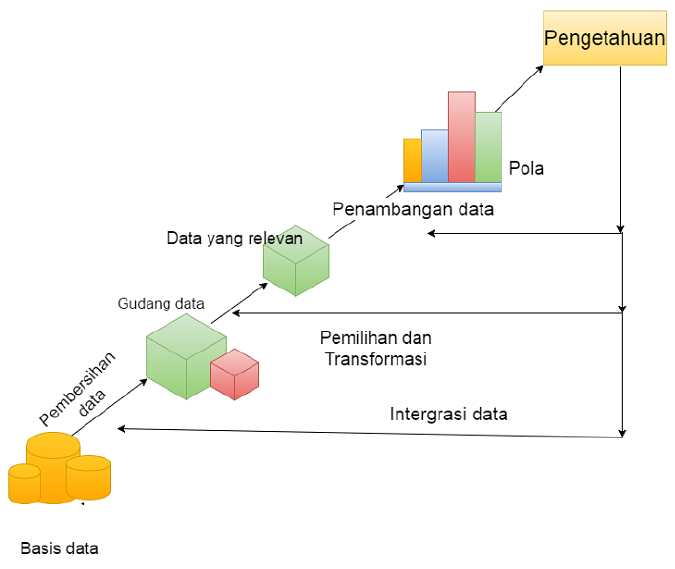
\includegraphics[scale=0.7]{GambarIO/langkah-data-mining}
	\caption[Langkah Penambangan Data]{Langkah Penambangan Data}
	\label{fig:Langkah Penambangan Data}
\end{figure}

Gambar 2.1 menyatakan langkah-langkah untuk menemukan pengetahuan dan proses-proses pengolahan data. Gambar 2.1 juga menyatakan bahwa setelah meraih pengetahuan, proses pencarian pengetahuan lebih lanjut juga dapat dilakukan kembali. Lihat anak panah pada Gambar yang merujuk pada langkah-langkah yang dapat dilakukan kembali untuk mendapatkan pengetahuan yang lebih mendalam. Berikut adalah proses-proses yang harus dilakukan dalam mencari pengetahuan baru \cite{DataMiningIntro:2015}:

\begin{itemize}
	\item{Pembersihan Data} \\
	Pembersihan data adalah fase yang membuang data yang tidak berguna (noise) dan data yang tidak relevan.
	\item{Integrasi data} \\
	Pada fase ini, beberapa sumber data yang heterogen digabungkan menjadi satu.
	\item{Pemilihan Data} \\
	Fase ini adalah fase dimana data dipilih, data yang relevan akan dipilih dari koleksi data pada fase sebelumnya.
	\item{Transformasi Data} \\
	Pada fase ini data yang dipilih ditransformasi sehingga memiliki bentuk yang layak untuk ditambang.
	\item{Penambangan Data} \\
	Fase ini adalah fase dimana teknik-teknik penambangan (termasuk Algoritma Apriori) digunakan untuk mencari pola yang memiliki potensi.
	\item{Evaluasi Pola} \\
	Pada fase ini, pola yang menarik akan diidentifikasi dan dianalisis sehingga dapat menghasilkan pengetahuan yang baru.
	\item{Penyimpulan Pengetahuan} \\
	Fase terakhir ini adalah fase dimana pengetahuan yang baru ditemukan itu direpresentasikan kepada pengguna.
\end{itemize}

\section{{\it Big Data}}

\subsection{Definisi {\it Big Data}}
{\it Big Data} merupakan suatu terminologi modern untuk sekumpulan data yang memiliki kesulitan tersendiri untuk diproses dengan cara tradisional (menggunakan satu buah komputer) \cite{zikopoulos2011understanding}. Dewasa ini perusahaan - perusahaan tengah menghadapi tantangan - tantangan yang ada pada {\it Big Data}, karena pertumbuhan data yang sudah semakin cepat dan grafik jumlah pengguna internet yang semakin menaik setiap saat. Mereka mendapatkan akses pada data/informasi tersebut tetapi tidak tahu cara mengambil informasi yang berguna pada data tersebut karena format dari data tersebut yang semi bahkan ada yang tidak terstruktur dan juga ukuran-nya yang sangat besar ; Cukup kebingungan apakah data tersebut akan berguna apabila terus disimpan. Karena, dapat dapat menyebabkan {\it memory overload}.

{\it Big Data} tidak melulu berasal dari internet, di dalam kehidupan kita sehari - hari sering kali kita berurusan dengan data, seperti data pada sensor sidik jari ketika absensi, data pembelian pada supermarket, data sensor kelembaban udara pada 10 tahun terakhir untuk memprediksi cuaca, kenaikan dan penurunan harga saham, {\it bitcoin}, dsb. {\it Big Data} menjadi topik yang diminati karena dengan data yang begitu banyak, dapat diteliti pola yang terjadi pada data tersebut selama beberapa kurun waktu tertentu untuk digunakan dalam menganalisis data dan membuat keputusan serta memberikan prediksi kemunculan data berikutnya dengan tingkat akurasi yang tinggi berdasarkan data yang dipelajari. Perusahaan - perusahaan saat ini tengah memulai untuk mengumpulkan setiap data yang dapat mereka peroleh dari {\it customer} untuk melihat pola aktifitas {\it customer} mereka dan membuat keputusan yang dapat menguntungkan perusahaan berdasarkan hal tersebut. Tentu saja hal ini tidak dapat dilakukan menggunakan teknik komputasi yang tradisional (menggunakan satu buah komputer berteknologi tinggi), karena biaya dan waktu yang terlalu mahal dan lama.

\subsection{Karakteristik {\it Big Data}}

 3 hal terpenting yang menjadi pokok permasalahan dalam {\it Big Data} adalah : 
\begin{enumerate}
	\item{Mengolah data yang berjumlah sangat besar} \\
	Ukuran data yang menjadi tantangan pada big data saat ini sangat besar, dari \textit{GigaByte} bahkan bisa mencapai puluhan \textit{PetaByte}.
	\item{Mengolah data yang memiliki tipe sangat bermacam - macam / variatif} \\
	Tipe dari data pada \textit{big data} sangat bermacam - macam. seperti: (1) angka, (2) tanggal, (3) \textit{string}\footnote{\textit{String} dalam pemrograman komputer adalah sebuah deret simbol. Tipe data string adalah tipe data yang digunakan untuk menyimpan barisan karakter}
	\item{Mengolah data dengan performa yang optimal}\\
	Tantangan yang terakhir pada \textit{big data} adalah kebutuhan untuk mengolah \textit{big data} dengan waktu dan sumber daya yang se-optimal dan se-efisien mungkin.
\end{enumerate}

Berikut merupakan beberapa contoh \textit{big data} dan pemanfaatannya diberbagai bidang \cite{JNetwork2012introductionBigData}:
\begin{enumerate}
	\item Pada bidang penerbangan dan transportasi, big data didapat dari data konsumsi bahan bakar dan pola lalu lintas di setiap armada secara nyata untuk meningkatkan efisiensi dan penghematan biaya.
	\item Pada sektor kesehatan, big data didapat dari berbagai catatan kesehatan elektronik pasien dari berbagai sumber, perawatan, demografi dan pencatatan khasiat obat sehingga dapat memberikan proses pengembangan obat yang lebih efisien dan lebih cepat.
	\item Pada sektor telekomunikasi, big data didapat dari penggunaan dan permintaan pengguna sehingga perusahaan telekomunikasi dapat menganalisis perilaku pengguna dan pola permintaan tersebut.
	\item Pada sektor media dan hiburan, big data didapat dari penggunaan media dan hiburan sehingga dapat dimanfaatkan untuk membantu pengambilan keputusan dan analisis prediktif dari penggunaan media dan hiburan tersebut.
\end{enumerate}


\section{Sistem Terdistribusi Hadoop}
	\subsection{Definisi Hadoop}
	Apache Hadoop merupakan platform \textit{open source} yang didirikan pada tahun 2006 untuk melakukan analisis pada big data. Hadoop merupakan software framework open source yang dapat menangani pertumbuhan jumlah data yang tinggi tanpa mempengaruhi performa kinerja-nya dengan sistem komputasi yang terdistribusi pada beberapa mesin yang dimiliki oleh Hadoop secara efisien \cite{Lam:2010:HA:1965594}. Hadoop terinspirasi dari MapReduce milik Google\cite{GoogleMR:2004} dan Google File System (GFS) \cite{GFS:2003}. \\
	Hadoop cluster\footnote{cluster merupakan sekelompok server} terdiri dari 2 node \footnote{node merupakan istilah teknik yang digunakan untuk menjelaskan suatu mesin atau komputer} yaitu \textit{Master Node} yang terdiri dari \textit{Namenode} dan \textit{Jobtracker daemon}\footnote{Daemon merupakan isitlah teknis yang digunakan untuk menjelaskan suatu proses yang berjalan secara background pada mesin linux} dan \textit{Slave Node} yang terdiri dari \textit{Datanode} dan \textit{Task Tracker}.
	
	\begin{figure}[ht]
			\centering
			\includegraphics[scale=0.7]{GambarIO/Master-Slave-Hadoop}
			\caption[Arsitektur master-slave]{Arsitektur master-slave}
			\label{fig:Arsitektur master-slave}
		\end{figure}
	
	\subsection{Fitur - fitur dari \textit{Hadoop} \cite{Lam:2010:HA:1965594}}
	\begin{enumerate}
		\item \textit{Cost Effective System}.
		Hadoop dapat diimplementasikan pada beberapa komputer biasa yang tidak memiliki spesifikasi terlalu tinggi. 
		\item \textit{Support Large Cluster or Node}.
		Jumlah node yang digunakan dapat mencapai ratusan bahkan ribuan node.
		\item \textit{Support Parallel Processing Data}.
		Proses yang dijalankan oleh hadoop dapat berjalan secara bersamaan pada cluster. Sehingga, kebutuhan akan waktu pengerjaan akan berkurang sebanding dengan banyaknya node yang dipakai.
		\item \textit{Distributed Data}.
		Hadoop akan menangani pendistribusian data kepada setiap node pada cluster dan melakukan replikasi data untuk seluruh cluster.
		\item \textit{Automatic Failover Management}.
		Jika cluster/node mengalami kerusakan (\textit{fail}), maka hadoop secara otomatis akan membebankan proses yang dikerjakan oleh cluster/node yang mengalami kerusakan tersebut kepada node node baru yang siap dan melakukan replikasi seluruh konfigurasi dan data dari node yang mengalami kerusakan tersebut ke node node baru.
		\item \textit{Data Locality Optimization}.
		Menggunakan konsep \textit{move-code-to-data}. Daripada menggunakan metode yang biasa digunakan, memasukan seluruh input ke dalam suatu kode, yang akan mengakibatkan \textit{bottleneck} pada jaringan transfer karena \textit{bandwidth} yang dibutuhkan tidak mampu melakukan transfer data yang sangat besar, lebih baik jika data tetap disimpan pada tempatnya,lalu kode kita yang dipindahkan ke tempat data tersebut berada. Karena, besaran file kode pasti akan jauh lebih kecil daripada data yang berukuran sangat besar. Sehingga, akan sangat menghemat waktu proses transfer yang berjalan.
	\item \textit{Heterogeneous Cluster}.
	Suatu *cluster, dapat terdiri dari komputer yang berbeda - beda spesifikasi, merek, maupun OS. Hal ini dapat memudahkan kita untuk membangun suatu \textit{commodity hardware}.
	\item \textit{Scalability}.
	Hadoop memiliki kemampuan untuk dapat menambah ataupun mengurangi node pada suatu cluster tanpa membuat server yang sedang berjalan \textit{down}.
	\end{enumerate}
	
	\subsection{Cara Kerja Hadoop}
	Hadoop menggunakan model pemrograman yang cukup sederhana untuk memproses data - data yang berukuran sangat besar melewati beberapa cluster mesin dan tempat penyimpanan memori yang terdistribusi. Oleh karena cara kerja hadoop yang menggunakan beberapa cluster mesin secara terdistribusi, besar kemungkinan untuk terjadi kegagalan dalam cluster tersebut pada saat ada proses yang sedang berjalan. Tetapi, kita tidak perlu khawatir dan mempersiapkan mekanisme penanganan untuk mengatasi hal tersebut, karena Hadoop sudah secara otomatis menangani hal tersebut agar apabila terjadi kegagalan (\textit{failure}) pada 1 atau lebih cluster/node, Hadoop akan mendistribusikan proses beserta seluruh sumber daya yang dibutuhkan oleh proses tersebut kepada mesin lain yang siap (\textit{available}). Hadoop sudah memiliki skema khusus untuk melindungi metadata dari kumpulan - kumpulan dataset yang berjumlah besar agar tidak hilang secara tidak sengaja, sehingga sangat aman digunakan (memiliki toleransi tinggi terhadap \textit{node failures}). Tahapan cara kerja hadoop adalah \cite{Holmes:2012:HP:2543981} : 
	\begin{enumerate}
		\item Membagi data input ke dalam bagian yang lebih kecil dan menyimpan setiap bagian dari data tersebut ke dalam node yang berbeda pada cluster.
		\item Mereplikasi setiap bagian data tersebut kepada beberapa node yang berada di cluster yang sama maupun yang berbeda. Secara default direplikasi sebanyak 3 kali (\textit{default replication factor is 3}).
		\item Menangani jalannya proses komunikasi diantara cluster. Seperti untuk mengakses replikasi data, jika dibutuhkan, pada cluster yang berbeda.
	\end{enumerate}
	\subsection{Elemen dari Hadoop}
	Hadoop memiliki 2 elemen penting, HDFS (\textit{Hadoop Distributed File System}) dan MapReduce. Keduanya sama - sama memiliki peran penting yang saling berhubungan untuk melakukan \textit{distributed computing}.
		\subsubsection{HDFS (Hadoop Distributed File System)}

HDFS merupakan sebuah sistem penyimpanan terdistribusi yang menyediakan akses throughput data yang tinggi. Akses throughput data yang tinggi memiliki arti bahwa HDFS dapat melakukan proses baca tulis data dalam skala yang besar. HDFS menciptakan beberapa replika dari setiap blok data dan mendistribusikannya pada seluruh cluster komputer untuk memungkinkan akses data yang dapat diandalkan dan cepat \cite{Holmes:2012:HP:2543981}. Dapat diandalkan dalam konteks ini bermaksud apabila sebuah node pada cluster Hadoop mengalami kegagalan yang menyebabkan data pada node tersebut corrupt, maka blok data tersebut tidak hilang karena selain node tersebut ada beberapa node lain yang menyimpan replika dari blok data tersebut. HDFS dapat melakukan komputasi dengan performa tinggi pada skala komputasi yang sangat besar \textit{(high-bandwidth computation)} dan biaya kapasitas penyimpanan terdistribusi yang dibutuhkan cukup rendah. HDFS didesain untuk data yang berukuran sangat besar GB to TB. HDFS memiliki default block size yang cukup besar, yakni 64 MB.

	HDFS terdiri dari 3 komponen utama yang berjalan secara \textit{background}, diantaranya adalah: 
		\begin{enumerate}
			\item \textit{NameNode}
			
			NameNode dapat disebut juga sebagai \textit{Master Node}. MasterNode biasanya hanya terdiri dari satu node saja. Tugas pertama dari MasterNode adalah untuk menyimpan seluruh metadata milik HDFS, seperti file name, file permission, file ownership, file location, dan id block pada file system. Tugas kedua dari MasterNode adalah untuk mengalokasikan 1GB pada RAM untuk melakukan pelacakan terhadap kurang lebih 1 juta file. Dan juga melakukan penyimpanan kepada disk, untuk backup data.
			\item \textit{DataNode}
			
			DataNode dapat disebut juga sebagai \textit{Slave Node}. Slave Node terdiri dari banyak node. SlaveNode bertanggung jawab untuk melakukan penyimpanan dan pengambilan data sesuai instruksi yang diperoleh dari NameNode. Secara periodik, SlaveNode memberikan status dari dirinya sendiri dan semua block file yang disimpan melalui \textit{*Heartbeat}. Slave Node menyimpan beberapa replikasi dari setiap file yang ada di dalam HDFS.
			\item \textit{Secondary NameNode}

			\begin{figure}[h]
			\centering
			\includegraphics[scale=0.5]{GambarIO/IX-Secondary-NameNode}
			\caption[Alur kerja Secondary NameNode dan NameNode]{Alur kerja Secondary NameNode dan NameNode}
			\label{fig:IX-Secondary-NameNode}
			\end{figure}

			%\begin{figure}
			%\centering
			%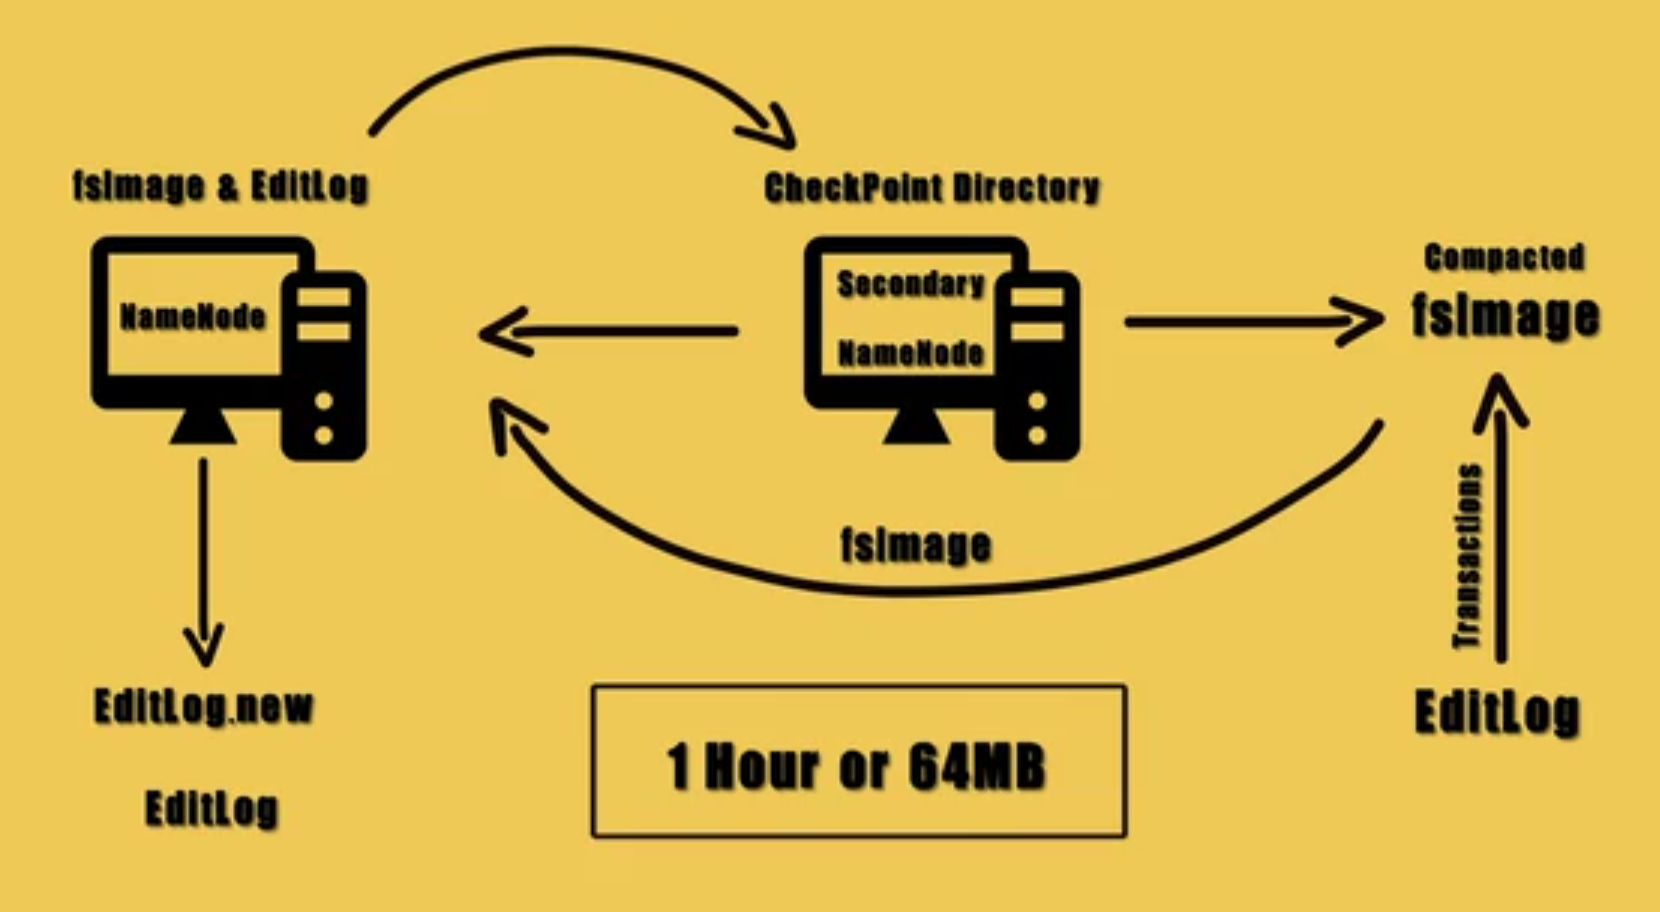
\includegraphics[scale=0.30]{Gambar/IX-Secondary-NameNode}
			%\caption[Alur kerja Secondary NameNode dan NameNode]{Alur kerja Secondary NameNode dan NameNode} 
			%\label{fig:IX-Secondary-NameNode}
			%\end{figure}

			Secondary NameNode merupakan MasterNode cadangan yang selalu aktif mencatat seluruh kegiatan dari NameNode untuk menjadi backup apabila server masternode yang utama mengalami kendala. Setiap transaksi yang dilakukan akan dicatat di dalam file editLog \footnote{File editLog adalah file yang menyimpan seluruh modifikasi yang dilakukan terhadap metadata}. Secondary NameNode akan memeriksa NameNode untuk menyimpan transaksi terbaru pada file editlog yang baru. Secondary NameNode akan membuat salinan dari fsImage \footnote{fsImage adalah file yang berisi snapshot lengkap mengenai metadata. Menyimpan semua blok yang dimiliki oleh suatu file dan file system property} dan editLog pada direktori \textit{checkpoint}. Setelah itu, ia akan menyimpan transaksi terbaru yang terjadi pada file editLog dan menyimpan seluruh informasi yang terbaru ke dalam \textit{compacted fsImage} baru. Secondary NameNode mengirim fsImage yang baru tersebut ke NameNode dan NameNode akan memilih fsImage yang baru tersebut. Proses ini akan berjalan setiap 1 jam sekali atau ketika besaran dari file editLog sudah mencapai 64MB. 
			Seperti yang tertera pada gambar 2.2. Ketika NameNode baru dijalankan, ia akan membuat file fsImage dan file editLog dari disk. Lalu menuliskan semua transaksi ke dalam metadata dari editLog yang telah di salin ke dalam RAM. Setelah selesai, versi baru dari fsImage akan dikembalikan dari memori RAM kepada memori disk.
		\end{enumerate}		
		
			%\begin{figure}
			%\centering
			%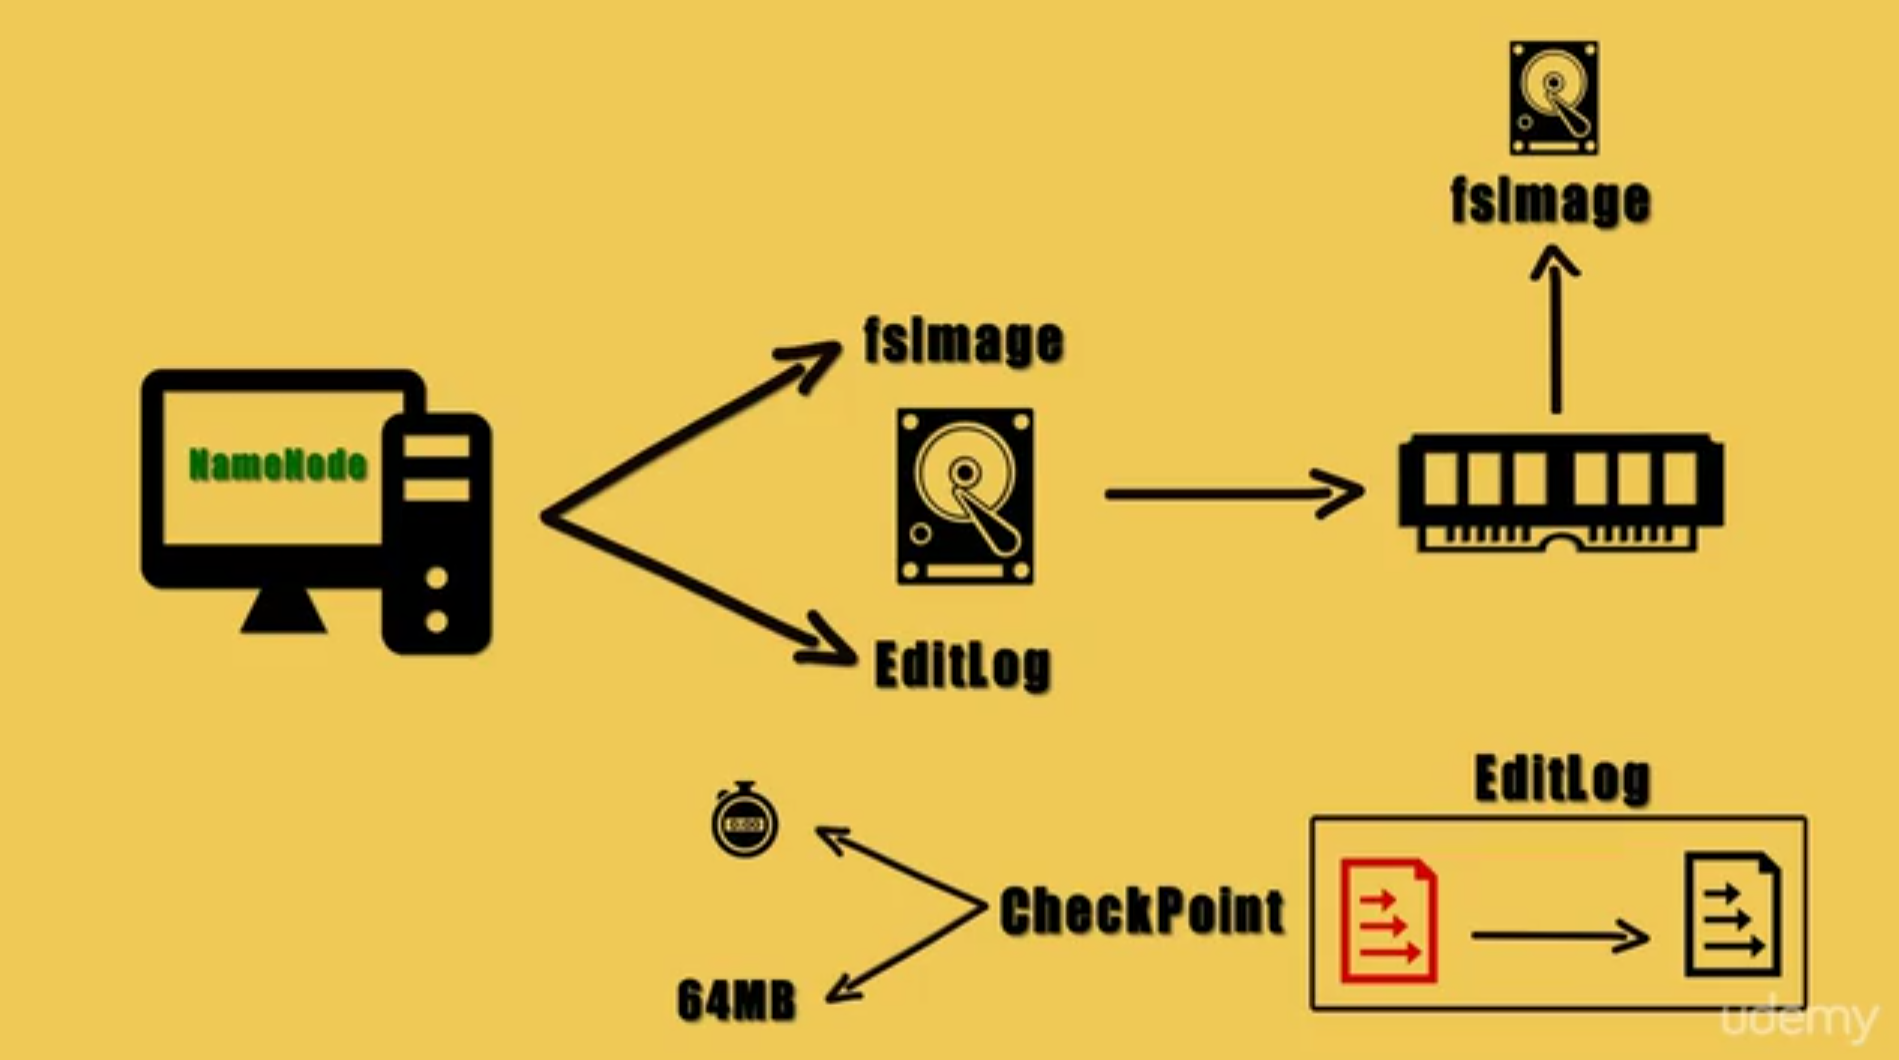
\includegraphics[scale=0.2]{Gambar/X-FileSystem-Metadata}
			%\caption[FileSystem Metadata pada NameNode dan Secondary NameNode]{FileSystem Metadata on NameNode and Secondary NameNode}
			%\label{fig:X-FileSystem-Metadata}
			%\end{figure}
			
			\begin{figure}[ht]
			\centering
			\includegraphics[scale=0.5]{GambarIO/X-FileSystem-Metadata}
			\caption[FileSystem Metadata pada NameNode dan Secondary NameNode]{FileSystem Metadata pada NameNode dan Secondary NameNode}
			\label{fig:FileSystem Metadata pada NameNode dan Secondary NameNode}
			\end{figure}
			
			HDFS memiliki 2 operasi yang penting, yaitu operasi baca dan operasi tulis dari dan ke HDFS. Berikut merupakan penjelasan lebih lanjut mengenai operasi baca dan operasi tulis dari dan ke HDFS.
		
		\paragraph{Membaca data dari HDFS}
			Untuk dapat membaca data dari HDFS, Hadoop Client membutuhkan "`Hadoop Client Library"' dan configurasi dari cluster. Mekanisme operasi baca data dari HDFS adalah sebagai berikut : (Ilustrasi pada gambar 2.4) : 
			
			\begin{figure}[ht]
			\centering
			\includegraphics[scale=0.54]{GambarIO/XI-Client-read-data-from-HDFS}
			\caption[Client membaca data dari HDFS]{Client membaca data dari HDFS}
			\label{fig:XI-Client-read-data-from-HDFS}
			\end{figure}
			
			%\begin{figure}
			%\centering
			%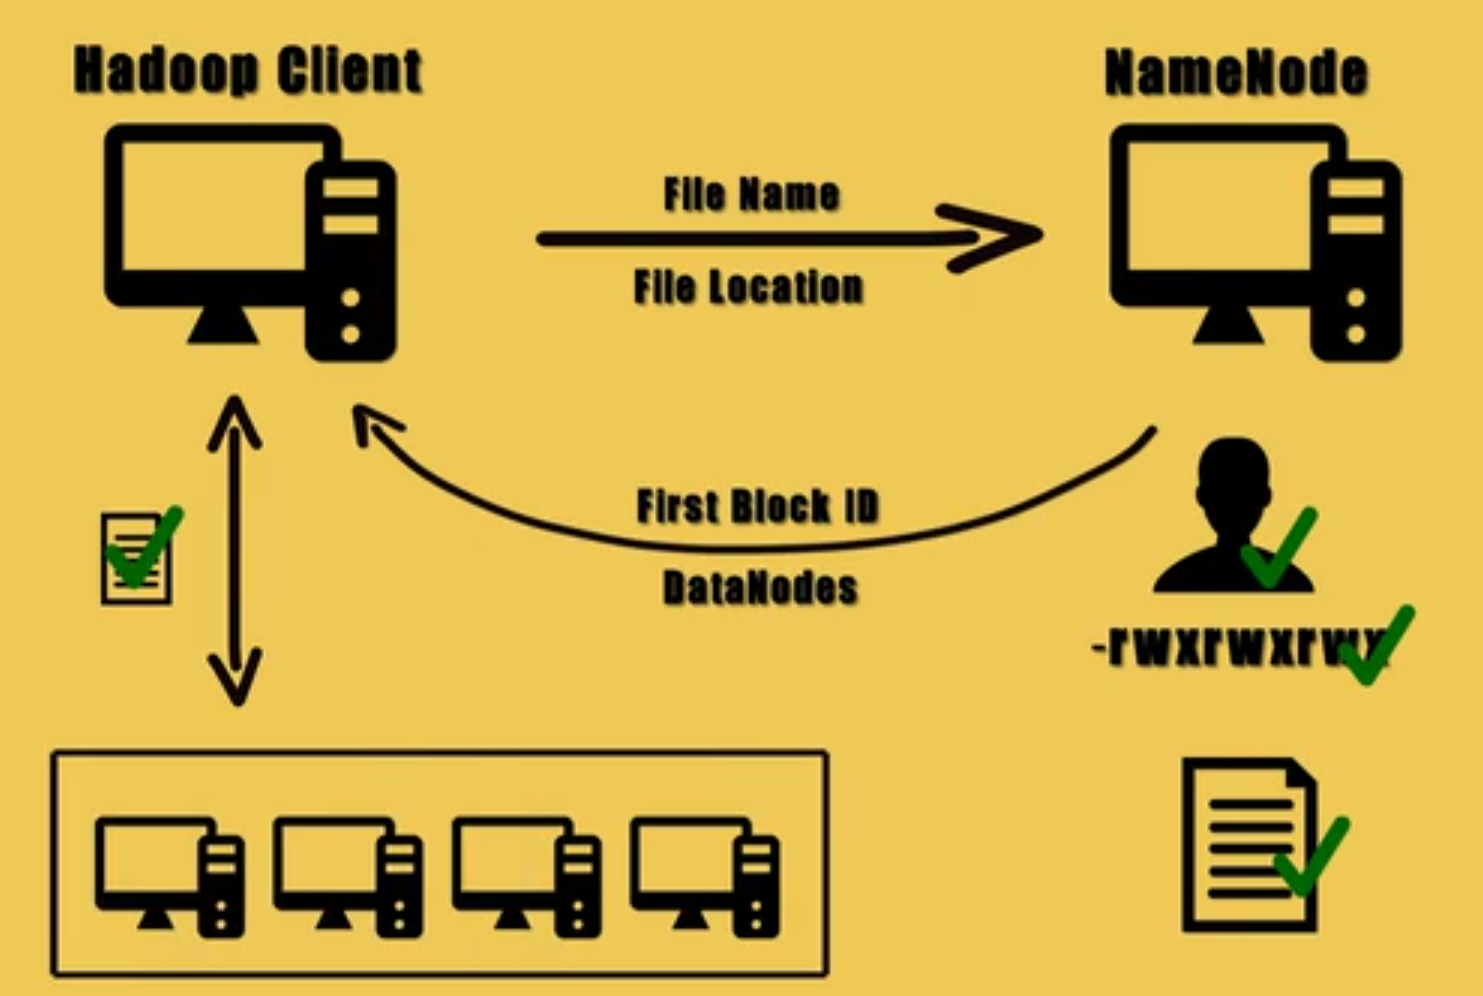
\includegraphics[scale=0.30]{Gambar/XI-Client-read-data-from-HDFS}
			%\caption[Client membaca data dari HDFS]{Client membaca data dari HDFS}
			%\label{fig:XI-Client-read-data-from-HDFS}
			%\end{figure}
			
			\begin{enumerate}
				\item Client menghubungi NameNode dan memberikan nama file lokasi pada file yang ingin dibaca.
				\item NameNode memvalidasi client untuk memeriksa permission yang dimiliki oleh user tersebut terhadap file yang diminta. 
				\item NameNode memberikan respon kembali kepada client dengan memberikan \textit{first block ID} \footnote{First block ID merepresentasikan tempat penyimpanan 64MB pertama dari data yang diminta tersebut. Memberikan informasi seperti pada rak dan DataNode yang menyimpan blok pertama pada file yang diminta.} dengan seluruh DataNode yang memiliki salinan/replikasi dari file yang dimintanya tersebut.
				\item Setiap DataNode yang memiliki salinan akan diurutkan berdasarkan yang terdekat sebelum dikirimkan kepada client.
				\item Setelah informasi - informasi di atas diterima oleh client, client dapat menghubungi secara langsung DataNode yang berhubungan dan membaca file nya.
				\item Jika DataNode yang digunakan pada saat melakukan operasi baca ke HDFS mengalami kerusakan, maka client akan langsung mengarahkan pembacaan ke DataNode yang lainnya yang memiliki replikasi dari data tersebut. Ilustrasi pada gambar 2.5.
				\item Jika replikasi yang dibutuhkan pada DataNode lainnya tidak ada, maka operasi baca akan mengalami kagagalan \textit{fail}. Ilustrasi pada gambar 2.6.
				
			\begin{figure}[h]
				\centering
				\includegraphics[scale=0.50]{GambarIO/Failure-Takeover-1}
				\caption[Failure takeover 1]{Failure takeover (success scheme)}
				\label{fig:Failure takeover (success scheme)}
			\end{figure}
			
			\begin{figure}[h]
				\centering
				\includegraphics[scale=0.50]{GambarIO/Failure-Takeover-2}
				\caption[Failure takeover 1]{Failure takeover (failure scheme)}
				\label{fig:Failure takeover (failure scheme)}
			\end{figure}
				
			\end{enumerate}		
		\paragraph{Menulis data ke HDFS}
		Gambar 2.6
		Mekanisme operasi tulis ke dalam HDFS :
		
		\begin{figure}[ht]
			\centering
			\includegraphics[scale=0.5]{GambarIO/XII-Client-Writing-data-on-to-HDFS}
			\caption[Client menulis data ke HDFS]{Client menulis data ke HDFS}
			\label{fig:XII-Client-Writing-data-on-to-HDFS}
		\end{figure}
			
		%\begin{figure}
			%\centering
			%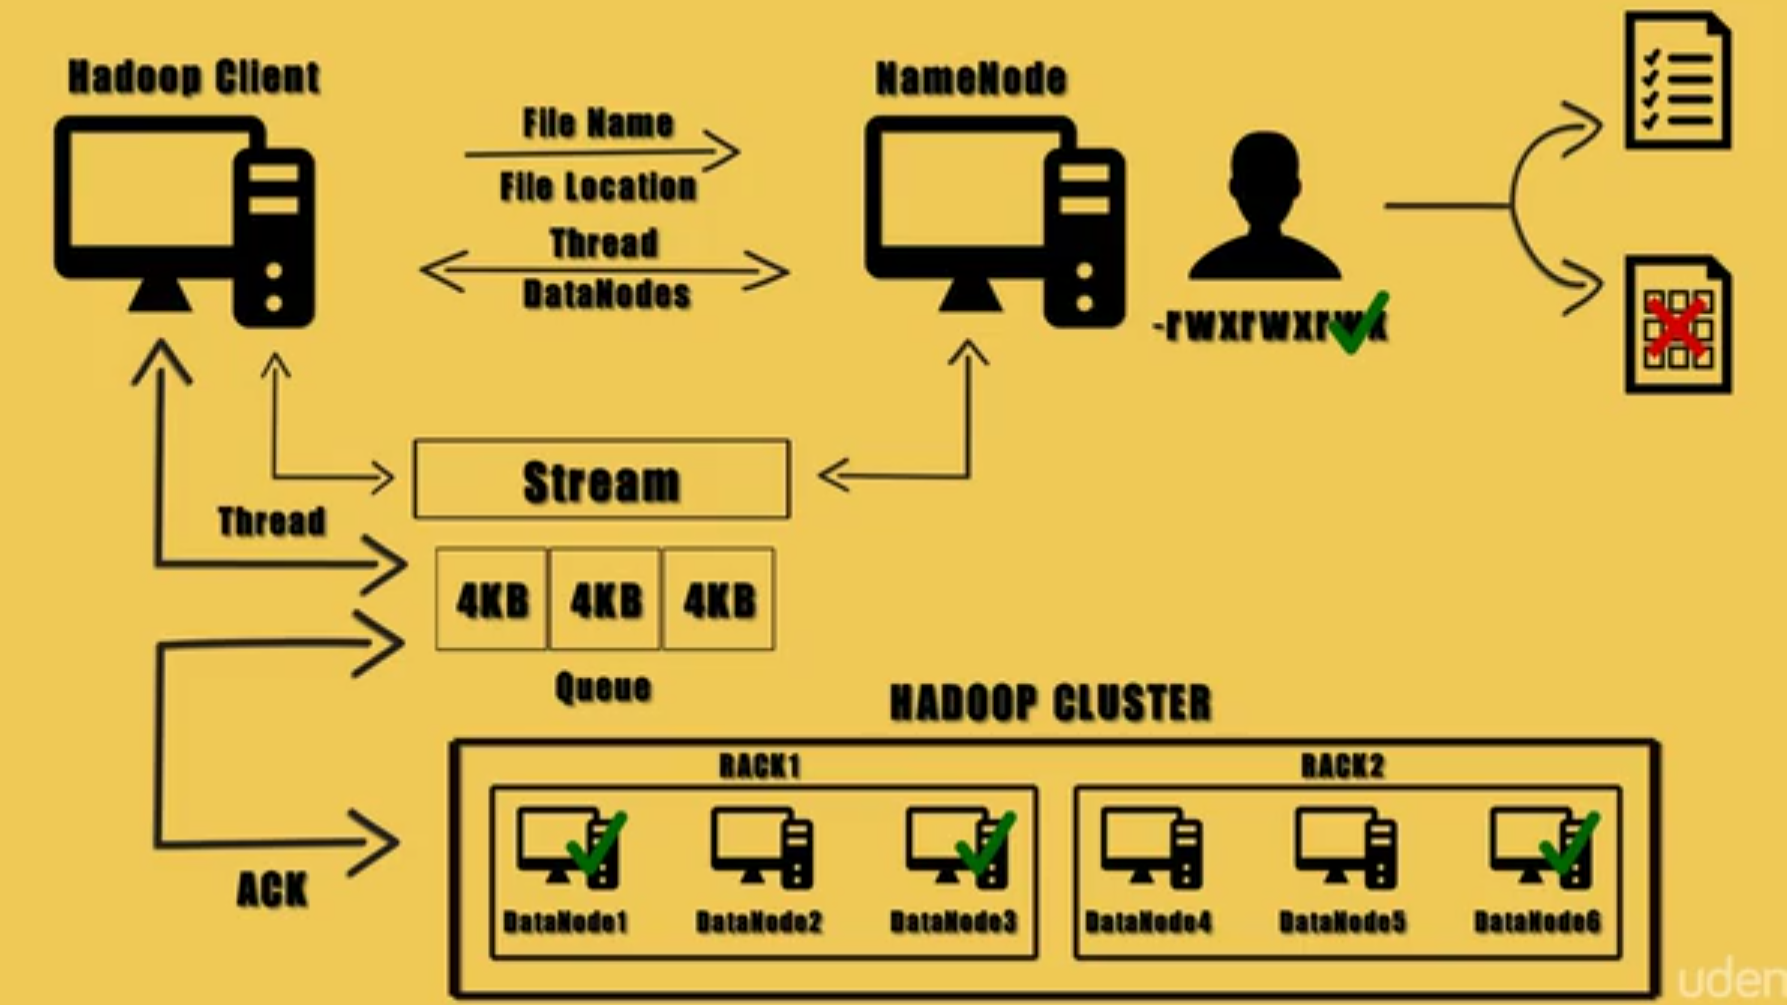
\includegraphics[scale=0.30]{Gambar/XII-Client-Writing-data-on-to-HDFS}
			%\caption[Client menulis data ke HDFS]{Client menulis data ke HDFS}
			%\label{fig:XII-Client-Writing-data-on-to-HDFS}
			%\end{figure}
			
		\begin{enumerate}
			\item Client akan menghubungi NameNode dan memberikan nama file dan lokasi yang diinginkan dari file yang akan di tulis.
			\item NameNode memvalidasi client untuk memeriksa permission yang dimiliki oleh user tersebut terhadap lokasi untuk penulisan file tersebut.
			\item NameNode akan membukakan sebuah stream untuk client melakukan operasi tulis. Data yang ditulis pada stream akan dipecah menjadi bagian - bagian kecil yang berukuran 4KB dan disimpan ke dalam queue.
			\item Client membuka thread yang berbeda yang akan bertanggung jawab untuk menuliskan data dari queue ke dalam HDFS.
			\item Thread akan menghubungi NameNode untuk meminta list dari DataNode yang dibutuhkan untuk menyalin replikasi dari data baru ini.
			\item Client akan menghubungi secara langsung DataNode pertama dan melakukan penulisan hingga sukses.
			\item Setelah sukses, tahap tersebut akan diulangi untuk setiap node yang mereplikasi data tersebut yang diberikan dari NameNode.
			\item Setelah selesai, ACK akan diberikan kepada client untuk memberi informasi bahwa penulisan telah selesai dan berhasil.
			\item Jika ketika sedang penulisan telah mencapai maksimum dari block size, maka client akan kembali menghubungi NameNode untuk meminta kumpulan DataNode berikutnya yang dapat dilakukan operasi tulis.
			\item Jika telah selesai, maka client akan menutup stream, lalu queue akan dibersihkan kembali, dan metada dari NameNode akan diupdate.
			\item Jika pada saat penulisan terjadi kegagalan, maka data yang dikirimkan setelah ACK terakhir yang diterima oleh client akan dikembalikan ke queue. Lalu didelegasikan ke DataNode yang baru dengan block id yang baru.
		\end{enumerate}
		
		%HDFS memiliki satu \textit{NameNode} untuk mengatur seluruh file system metadata dan beberapa \textit{DataNodes} untuk menyimpan dataset yang sudah ter-partisi (direpresentasikan sebagai b1,b2,b3,dst.). \\
		%Ketika sekumpulan dataset masuk kedalam HDFS, HDFS akan mendistribusikan penyimpanan data pada tiap cluster yang berhubungan agar data tidak bercampur aduk dan dapat diambil dengan cepat. Biasanya HDFS memiliki blok data sebesar 64-128MB dan setiap partisi-nya akan di copy/replika-kan ke beberapa node secara acak, agar jika terjadi kegagalan dapat dengan cepat di-\textit{handle} dengan mesin lainnya.
		
%\begin{figure}
%\centering
%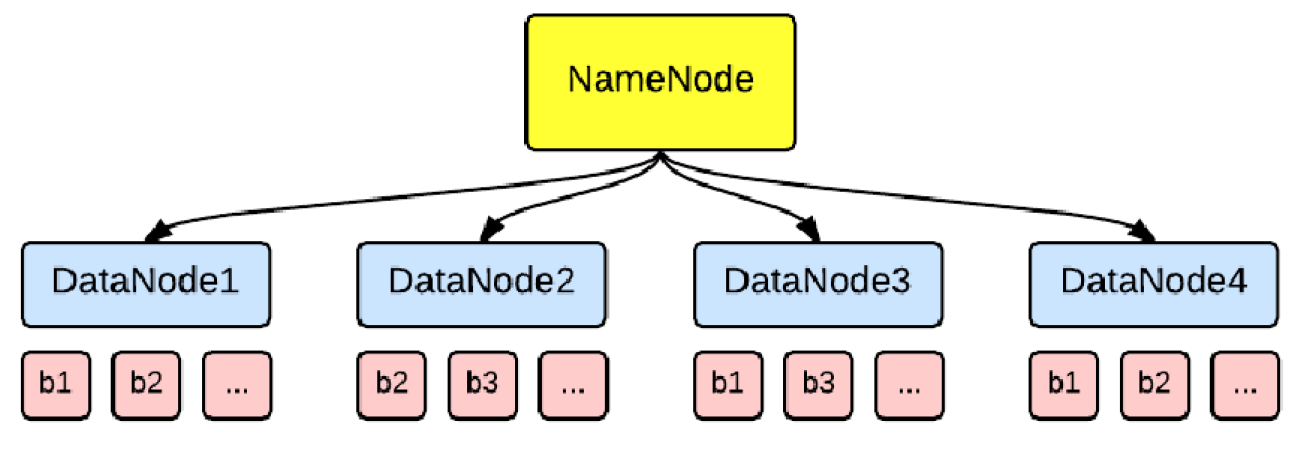
\includegraphics[scale=0.38]{Gambar/hdfs_arch}
%\caption[Arsitektur Hadoop Distributed File System (HDFS)]{Arsitektur Hadoop Distributed File System (HDFS)} 
%\label{fig:hdfs_arch}
%\end{figure}
				
\subsubsection{MapReduce}

\begin{figure}[h]
	\centering
	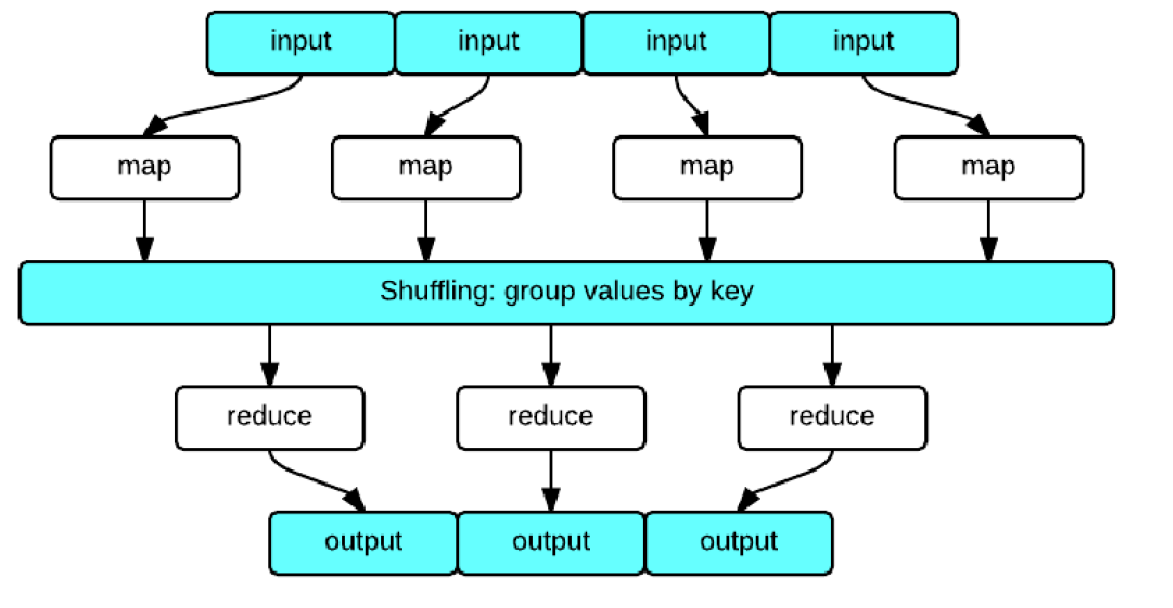
\includegraphics[scale=0.43]{GambarIO/map_reduce}
	\caption[Ilustrasi framework MapReduce]{Ilustrasi framework MapReduce}
	\label{fig:map_reduce}
\end{figure}
		
		MapReduce merupakan framework yang dirancang untuk memproses data secara paralel terdistribusi yang memiliki performa dan efisiensi yang sangat tinggi. Jenis pekerjaan pada fase map dan reduce yang dapat dikerjakan oleh framework ini merupakan jenis pekerjaan yang tidak memiliki hubungan berkesinambungan di antara  tiap proses-nya, sehingga dapat berjalan secara bersama - sama (\textit{concurrent}). Hadoop membagi/memecah seluruh dataset yang ada ke dalam beberapa partisi dan mendistribusikannya ke dalam kelompok/\textit{cluster}. MapReduce memproses data di setiap server terhadap blok - blok data yang sudah dibagikan sebelumnya, sehingga akan sangat menghemat waktu pekerjaan yang dihabiskan \cite{Lam:1965594:HA}. \\
		Terdapat 3 fase utama pada MapReduce, yaitu fase \textit{map}, fase \textit{shuffle}, dan fase \textit{reduce}. 
		\begin{enumerate}
			\item Pada fase \textit{map}, melakukan \textit{convert} tiap partisi dari input kedalam pasangan \textit{key/value} (seperti pada struktur data HashMap) lalu menggabungkan setiap \textit{value} yang memiliki \textit{key} yang sama.
			\item Pada fase shuffle, hasil keluaran dari fase Map akan di sort berdasarkan key dan pasangan \textit{key/value} tersebut akan di kirimkan ke reducer node yang menerima pasangan \textit{key/value} yang sesuai.
			\item Pada fase \textit{reduce}, algoritma menerima sebuah pasangan key dengan himpunan dari value yang memiliki hubungan dengan key tersebut, lalu melakukan suatu proses yang nantinya akan menjadi keluaran dari program MapReduce.
		\end{enumerate} 
		
	Beberapa komponen utama dari \textit{MapReduce} terdiri dari \textit{JobTracker} dan \textit{TaskTracker}.
	\begin{itemize}
		\item \textit{JobTracker} berperan sebagai \textit{master} dari \textit{MapReduce}. \textit{JobTracker} mengelola pekerjaan dan sumber daya dalam \textit{cluster} (\textit{TaskTracker}). \textit{JobTracker} berusaha untuk menjadwalkan proses setiap \textit{map} dan \textit{reduce} pada \textit{TaskTracker} sedekat mungkin dengan \textit{DataNode} yang memiliki blok data yang diproses.
		\item \textit{TaskTracker} adalah slave yang ada pada setiap node. \textit{TaskTracker} bertanggung jawab untuk menjalankan proses \textit{map} dan \textit{reduce} seperti yang diperintahkan oleh \textit{JobTracker}.
	\end{itemize}
		
		Komponen utama lainnya setelah release versi terbaru hadoop 2 dari MapReduce adalah Apache YARN (\textit{Yet Another Resource Negotiator}). YARN bertanggung jawab untuk mengawasi \textit{resource} yang tersedia pada seluruh node dan memantau status dari setiap \textit{TaskTracker} yang ada pada setiap node dan status dari pekerjaannya. YARN sebagai arsitektur baru dari Apache hadoop 2 membagi dua fungsi utama dari JobTracker/TaskTracker pada MapReduce menjadi beberapa entitas yang terpisah, diantaranya adalah: 
		\begin{itemize}
			\item \textit{Resource Manager} di \textit{node master}, yang bertugas untuk mengawasi dan mengatur seluruh \textit{resource} yang tersedia dan digunakan pada seluruh node.
			\item \textit{Application Master} di setiap aplikasi, yang berfungsi untuk memantau status dari setiap \textit{TaskTracker} yang ada pada setiap node dan status dari pekerjaannya dan juga untuk negosiasi resource dengan \textit{ResourceManager} dan kemudian bekerja sama dengan \textit{NodeManager} untuk mengeksekusi dan memonitor \textit{tasks}.
			\item \textit{NodeManager} di \textit{Agen-Framework} setiap \textit{node slave}, yang bertanggung jawab terhadap \textit{container}, dengan memantau penggunaan resource/sumber daya dari container(cpu, memori, disk, jaringan ) dan melaporkannya pada ResourceManager.
			\item \textit{Container} di setiap aplikasi yang jalan di \textit{NodeManager}, sebagai wadah penyimpanan data/file.
		\end{itemize}
		
\begin{figure}[H]
\centering
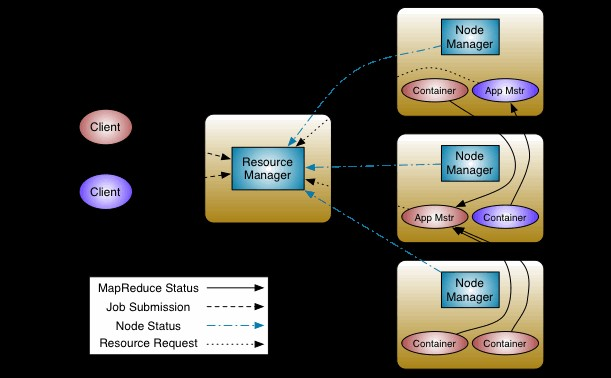
\includegraphics[scale=0.6]{YARN-Architecture}
\caption[Arsitektur YARN-1]{Arsitektur YARN-1}
\label{fig:Arsitektur YARN-1}
\end{figure}
		
Pada YARN setiap pekerjaan akan memiliki JobTracker-nya masing - masing dan pada suatu cluster dapat memiliki beberapa JobTracker yang sedang bekerja. Setiap JobTracker pada node yang berbeda akan bisa berjalan pada software yang berbeda. Hal ini yang mendukung model  dari \textit{Heterogeneous Cluster}.

%\begin{figure}[ht]
%\centering
%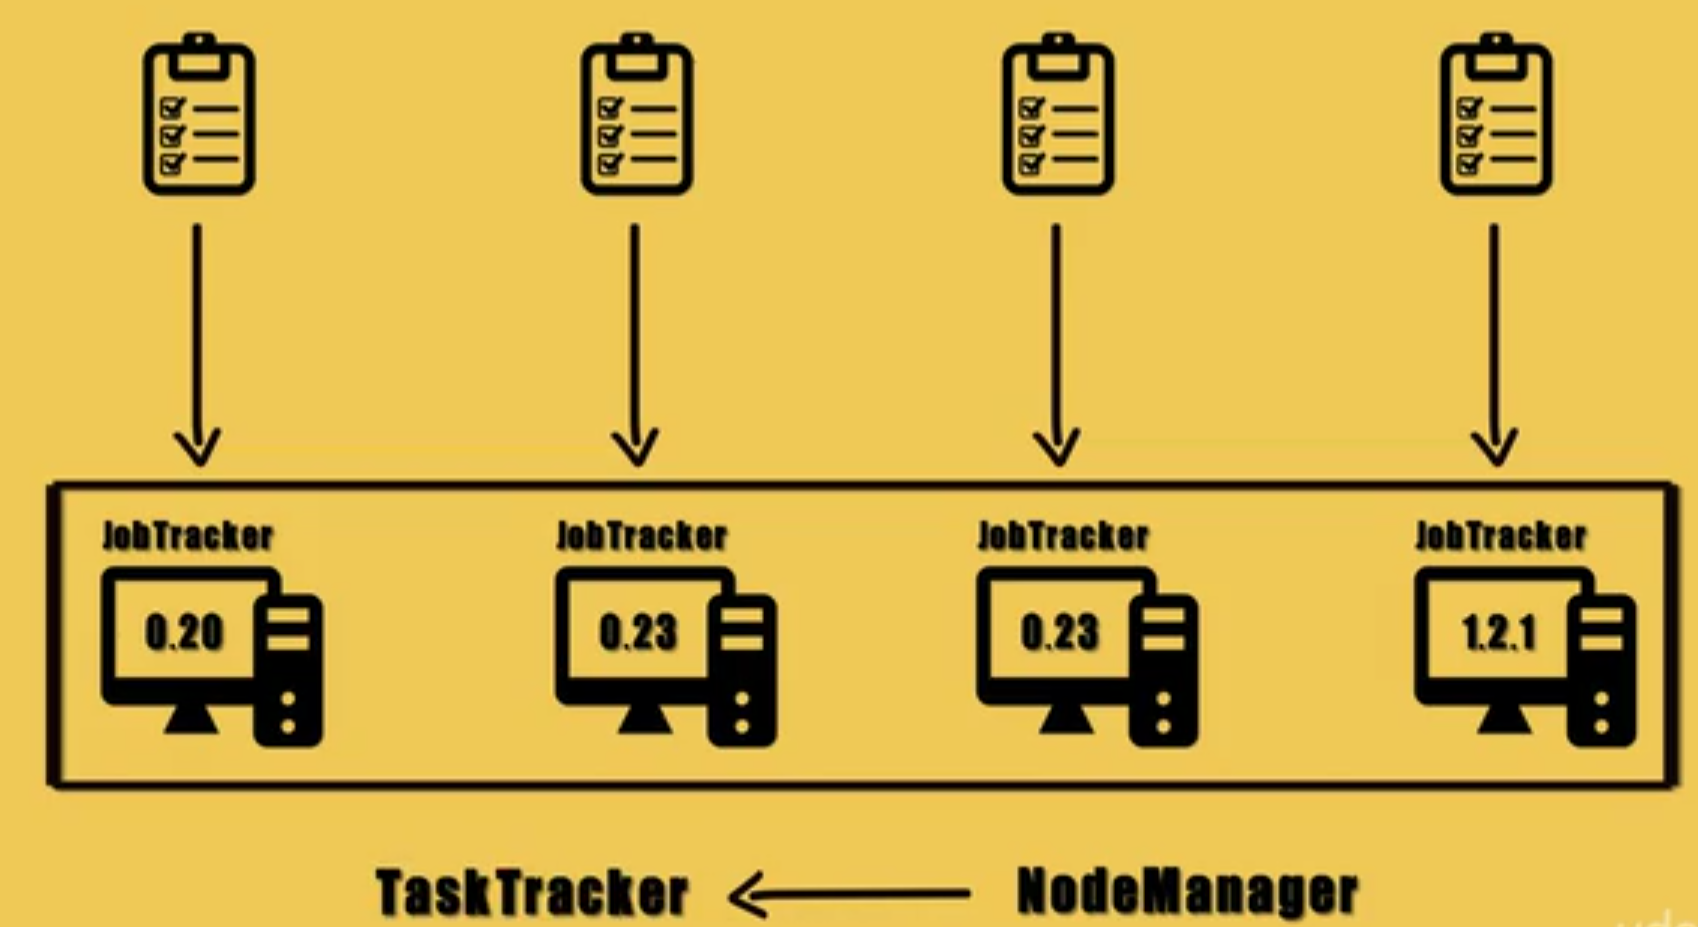
\includegraphics[scale=0.2]{Gambar/II-YARN-3-Het-Cluster}
%\caption[Arsitektur YARN-2]{Arsitektur YARN-2}
%\label{fig:Arsitektur YARN-2}
%\end{figure} 

\begin{figure}[h]
	\centering
	\includegraphics[scale=0.5]{GambarIO/Hetergenous-Cluster-YARN}
	\caption[Arsitektur YARN]{Arsitektur YARN : Heterogenous Cluster YARN}
	\label{fig:Arsitektur YARN : Heterogenous Cluster YARN}
\end{figure}


Map-Reduce ada pada setiap DataNode pada cluster Hadoop. Setiap program Map-Reduce mengerjakan atau mengolah data - data yang terdapat pada DataNode-nya. Map-Reduce ditulis dengan bahasa Java, sehingga untuk setiap abstraksi dan aturan pada pembuatan kode mengikuti bahasa Java. Selain itu, Map-Reduce milik Hadoop dibuat untuk memudahkan programmer sehingga hanya perlu berfokus pada dua buah fase yang digunakan saja, yaitu fase map dan reduce. Sedangkan untuk fase Shuffle dan Sort sudah ditangani secara otomatis oleh framework Hadoop. Berikut merupakan penjelasan lebih lanjut mengenai mapper dan reducer yang digunakan pada fase map dan fase reduce.

\paragraph{Mapper} 

Mapper berfungsi untuk memetakan data yang diberikan kepada MapReduce. Dalam Hadoop, Mapper berada pada setiap node dan bekerja menggunakan data yang berada pada masing-masing node. Hal ini dapat mengurangi lalulintas data yang terjadi pada cluster Hadoop karena tidak ada perpindahan data antar node. Mapper membaca data dalam bentuk pasangan key dengan value dan mengeluarkan nol atau lebih pasangan key dengan value dalam bentuk list yang disimpan pada penyimpanan local di DataNode (bukan dalam bentuk HDFS).

\paragraph{Reducer}

Reducer berfungsi untuk mengurangi data yang tidak diperlukan (misal : data yang berulang) atau menyatukan data yang dapat disatukan dari hasil Mapper. Jumlah Reducer pada sebuah MapReduce pada sebuah node dapat lebih dari satu. Reducer menerima sebuah list pasangan key dengan value dari Mapper yang terurut berdasarkan keynya. Hasil keluaran dari Reducer berupa nol atau lebih pasangan key dan value yang sudah final. Hasil tersebut sudah disimpan di HDFS. Sebelum diterima oleh Reducer, seluruh hasil dari Mapper melalui sebuah tahap yang dinamakan shuffle and sort. Tujuan dari tahap ini adalah memastikan bahwa semua value dengan key yang sama masuk ke reducer yang sama dan list pasangan key dan value yang diterima terurut pada berdasarkan key.

\paragraph{Cara kerja MapReduce}

%\begin{figure}[h]
%\centering
%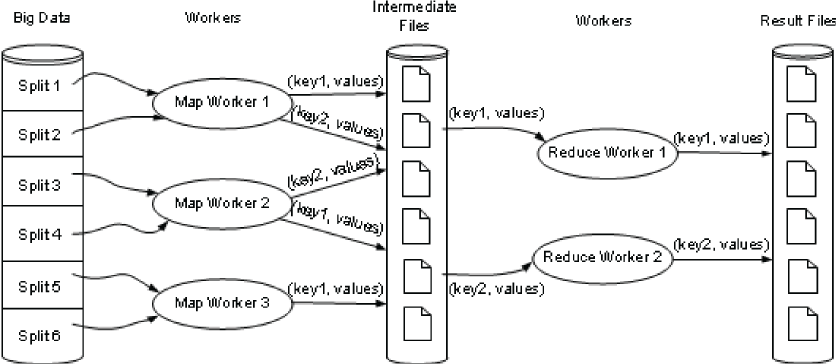
\includegraphics[scale=0.35]{Gambar/MapReduceWorks-google}
%\caption[MapReduce Works]{MapReduce Works}
%\label{fig:MapReduce Works}
%\end{figure}

\begin{enumerate}
	\item MapReduce akan membaca setiap line dari input yang akan dijadikan sebagai input dari fase Map. Setiap line yang dibaca oleh fase Map merupakan pasangan \textit{key/value} dari line yang menjadi input tersebut (sebagai value) dan offset dari text tersebut terhadap awal file (sebagai key).
	\item Fase map akan dijalankan sesuai apa yang kita perintahkan/implementasikan pada program Map yang dibuat. Keluaran dari fase Map merupakan pasangan \textit{key/value} yang telah diproses.
	\item Keluaran dari fungsi map sebelum dijadikan sebagai hasil input dari fungsi reduce akan diproses oleh fase \textit{Shuffle and Sort}. Pada fase Shuffle and Sort, hasil keluaran dari fungsi map akan diakumulasi dan pengurutan. Untuk setiap key yang sama akan dikelompokan kedalam sebuah pasangan \textit{key/value} baru yang isinya merupakan key dari input tersebut dan value nya merupakan list dari seluruh pasangan \textit{key/value} yang memiliki key sama.
	\item Setelah output fungsi map melewati proses shuffle and sort, maka output tersebut akan terurut berdasarkan key. Sehingga, reducer akan dengan tepat melihat key dan seluruh value yang bersangkutan, yang sudah ditetapkan untuk diproses pada reducer node yang akan menjalankan tugasnya.
	\item Pada fase reduce, akan dijalankan fungsi reduce yang sudah diimplementasikan sebelumnya untuk memproses pasangan dari \textit{key/list-of-value-key} menjadi hasil yang dibutuhkan.
\end{enumerate}

		
--------------------------------------------------------------------------------------------------

\section{\textit{Naive Bayes Classifier}}
	
	 Naive Bayes merupakan salah satu metode mesin learning yang digunakan pada teknik data mining menggunakan metode perhitungan peluang. Konsep dasar yang digunakan oleh Naive bayes adalah Teorema Bayes, yaitu teorema dalam statistika untuk menghitung peluang suatu kejadian dari beberapa kejadian lainnya. Bayes Optimal Classifier menghitung peluang dari satu kelas dari masing-masing kelompok atribut yang ada dan menentukan kelas mana yang paling optimal. Algoritma Naive Bayes melakukan klasifikasi berdasarkan pada teorema Bayes' seperti berikut : 

\begin{equation}
P(A|B) = \dfrac{P(B|A)P(A)}{P(B)}
\end{equation}

	Teori bayes memiliki asumsi bahwa probabilitas P(A|B) atau peluang kejadian A bila B terjadi tidak saling berhubungan dengan setiap kemungkinan dari nilai B yang diberikan (\textit{naive}). Hal ini disebut sebagai \textit{class conditional independence} . Sehingga memudahkan perhitungan yang dilakukan pada saat klasifikasi. Kemungkinan terjadinya kejadian A bila diberikan kejadian B dapat dihitung dengan menggunakan rumus diatas, yaitu mengalikan peluang dari kejadian B jika diberikan kejadian A dikalikan dengan peluang seluruh kejadian A dan dibagi dengan peluang dari seluruh kejadian B.\\

Berdasarkan teori Bayes, untuk dataset $d$ dan sebuah kelas $c$, didapatkan : \\

\begin{equation}
P(c|d) = \dfrac{P(d|c)P(c)}{P(d)}
\end{equation}

\begin{itemize}
	\item $P(c|d)$ merupakan peluang dari kemunculan suatu kelas/kelompok tertentu jika diberikan suatu dataset $d$
	\item $P(d|c)$ merupakan peluang suatu dataset tertentu jika diberikan suatu kelas $c$
	\item $P(c)$ merupakan probabilitas dari kelas
	\item $P(d)$ merupakan probabilitas dari dokumen/dataset
\end{itemize}

Untuk menghitung nilai $P(c|X)$ (\textit{X merupakan dataset yang digunakan sebagai predictor}) dengan mengasumsikan bahwa masing - masing atribut tidak saling bergantung dengan atribut lainnya \textit{class conditional independence}, maka didapat : 
\begin{equation}
	P(c|X) = P(x_1|c) P(x_2|c) ... P(x_n|c) P(c)
\end{equation}

Sebuah dataset dapat ditentukan klasifikasi-nya dengan algoritma naive bayes setelah dihitung semua kemungkinan dari nilai $P(c_k|X)$ dan untuk nilai keluaran yang paling besar akan dipilih menjadi kelas yang paling optimal dari dataset tersebut.

\textit{MAP Maximum A Posteriori}
		\begin{equation}
			C_{MAP} = \underset{c \in C}{ argmax } P(c|d) = \underset{c \in C}{ argmax } \dfrac{P(d|c) P(c)}{P(d)} = \underset{c \in C}{ argmax } P(d|c) P(c)
		\end{equation} \\
	
\section{Framework Yang Digunakan Dalam Membangun Perangkat Lunak}

\subsection{\textit{Spring Framework}}
\label{subsec:Spring Framework}

\textit{Spring Framework} adalah salah satu framework\footnote{framework adalah tools yang bisa digunakan untuk mengembangkan cakupan luas dari arsitektur-arsitektur yang berbeda \cite{setiawan2009pemilihan}} untuk aplikasi berbasis Java yang dapat digunakan untuk membangun sebuah aplikasi berskala besar. Model yang digunakan pada perangkat lunak yang dibangun adalah \textit{spring framework web application} yang memiliki ekstensi untuk membuat server pada aplikasi berbasis web dengan J2EE (Java 2 Enterprise Edition) \cite{SpringCommerceToha:2010}. Dengan Spring, kita bisa mengembangkan aplikasi enterprise dan berbasis web. Spring termasuk portable karena aplikasi yang dikembangkan dapat berjalan pada JVM manapun. Terdapat beberapa cara yang disediakan oleh spring untuk melakukan deploy aplikasi kita, seperti: 
\begin{enumerate}
	\item Melakukan deploy aplikasi dengan menggunakan mode standalone (menggunakan server bawaan dari \textit{spring}),
	\item Melakukan deploy aplikasi pada aplikasi server (menggunakan aplikasi web server dari luar, seperti \textit{Apache Tomcat Web Application}),
	\item Melakukan deploy aplikasi dengan menggunakan \textit{cloud PaaS}\footnote{\textit{Platform as Service merupakan sebuah platform untuk mengembangkan, menjalankan, dan mengatur aplikasi kita tanpa melewati serangkaian konfigurasi yang rumit layaknya \textit{dedicated server} pada umumnya}} (\textit{Platform as Service}, seperti \textit{Pivotal Web Service}).
\end{enumerate}
Spring menyediakan model pemrograman terbuka yang komprehensif, kohesif, mudah dipahami serta memiliki \textit{library} yang lengkap untuk melakukan integrasi ke \textit{service - service} lain seperti \textit{Hadoop-client Library}, \textit{Mysql-connector Library}, dsb. Inti dari framework ini lebih kepada untuk membangun aplikasi web, mengatur manajemen transaksi, akses data, messaging, pengujian dsb. Kita bisa mengembangkan aplikasi web berbasis MVC dan \textit{Web-Service} framework \textit{REST-ful}\footnote{REST merupakan \textit{standard} dalam arsitektur web yang menggunakan Protocol HTTP untuk pertukaran data.  Konsep REST menekankan bahwa komunikasi yang terjadi antara \textit{client} dan \textit{server} hanya sebatas melakukan \textit{request} dan memberikan \textit{response} saja.} (\textit{Representational State Transfer}).

\textit{Design pattern} yang digunakan pada perangkat lunak yang dibuat akan menggunakan konsep MVC (\textit{model view controler}). Spring memiliki fitur khusus untuk membuat web berbasiskan \textit{design pattern} MVC. Berikut merupakan ilustrasi\footnote{Gambar diambil dari \url{https://docs.spring.io/spring/docs/current/spring-framework-reference/html/images/mvc.png.pagespeed.ce.tmIzOTr1gg.png}} dari \textit{request workflow} pada \textit{Spring Web} MVC.
\begin{figure}[h]
	\centering
	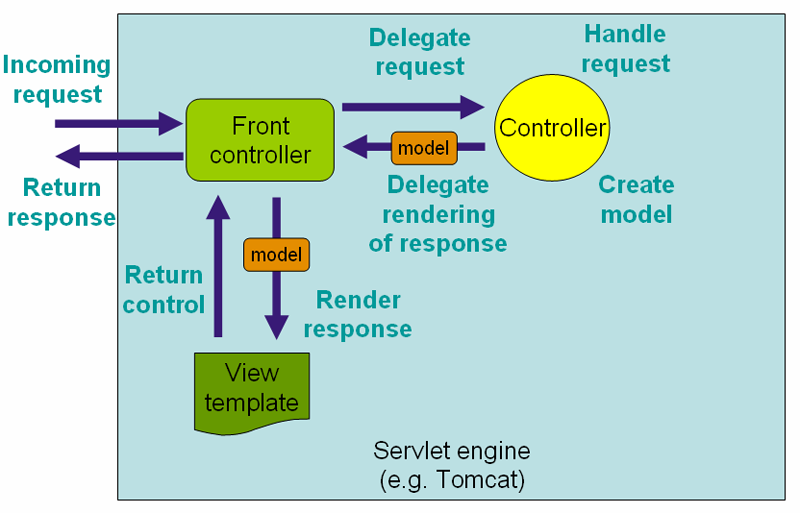
\includegraphics[scale=0.5]{GambarIO/mvc_springdocs}
	\caption[Request Processing Workflow Spring MVC]{\textit{Request Processing Workflow Spring MVC}}
	\label{fig:Request Processing Workflow Spring MVC}
\end{figure}

\begin{enumerate}
	\item \textit{\textbf{Model}} melakukan enkapsulasi dari data yang ada pada aplikasi dan secara umum akan berisi POJO\footnote{Istilah POJO (\textit{Plain Old Java Object}) digunakan untuk menunjukkan objek java yang hanya berisi variable serta \textit{accessor} dan \textit{mutator} -nya tanpa ada method proses lainnya}.
	
	\item \textit{\textbf{View}} bertanggung jawab untuk melakukan \textit{rendering} data dengan view HTML yang diinginkan, lalu akan men-\textit{generate} output berupa HTML yang dapat diinterpretasikan oleh \textit{browser}.

	\item \textit{\textbf{Controller}} bertanggung jawab untuk memproses \textit{request} dari user dan lalu perlu memberikan model sesuai dengan yang diminta yang nantinya akan diberikan ke \textit{view} untuk proses \textit{rendering}.
	
\end{enumerate}

%\textit{Design pattern} perangkat lunak yang dibangun akan mengusung konsep dari MVC milik \textit{spring} dan beberapa tambahan \textit{layer - layer} untuk mempermudah jalannya perangkat lunak nantinya. Berikut merupakan ilustrasi

\subsection{\textit{Maven} \cite{MengenalMaven2015EGunawan}}
Apache Maven adalah software build tools / project management yang dibangun dibawah \textit{Apache Software Foundation} yang digunakan untuk melakukan proses building project. Jadi, ketika project akan dibuild menggunakan Maven, project tersebut bisa kita buka menggunakan IDE lain.

Selain itu, keuntungan menggunakan maven adalah mendukung dependency management. Artinya, ketika kita membutuhkan suatu library ke dalam project, kita tidak perlu mendownloadnya manual, kemudian dimasukkan ke dalam project. Kita tinggal memasukkan  ependency-nya, dan maven akan menanganinya.  Dengan begini, ukuran project menjadi lebih kecil karena tidak memasukkan library ke dalam project.

Untuk mendownload Apache Maven bisa langsung ke websitenya di \url{http://maven.apache.org/}. Versi terbaru dari Apache Maven adalah 3.5.0.

\subsection{\textit{Thymeleaf} \cite{CogoluegnesIntroducing:2013}}
\textit{Thymeleaf} merupakan \textit{template-engine open source} yang dapat melakukan \textit{rendering} HTML pada \textit{server-side}. Thymeleaf adalah Java XML template engine / XHTML / HTML5 yang dapat bekerja baik di web (\textit{Servlet-based}) maupun lingkungan yang bukan web. Hal ini lebih cocok untuk melayani XHTML / HTML5 pada \textit{layer} tampilan aplikasi berbasis web MVC, tetapi dapat memproses file XML bahkan di lingkungan offline. \textit{Template engine} ini menyediakan integrasi penuh dengan \textit{Spring Framework}. 

Dalam aplikasi web Thymeleaf bertujuan untuk menjadi pengganti lengkap untuk JSP, dan menerapkan konsep Natural Template: file template yang bisa langsung dibuka di browser dan yang masih menampilkan dengan benar sebagai halaman web.

Sebagai \textit{framework open source}, \textit{Thymeleaf} memiliki lisensi Apache 2.0 



		%\paragraph{Perhitungan pada \textit{Naive Bayes Classifier}}
		%Untuk mengetahui perhitungan pada algoritma \textit{Naive Bayes}, pertama kita perlu mengetahui dan mengikuti table kontigensi 2-by-2. Terdapat 4 kondisi/\textit{state} dari setiap data yang kita evaluasi. Jika data sebenarnya merupakan instansiasi dari klasifikasi yang sedang dicoba dan klasifikasi yang kita lakukan pun menyatakan bahwa data tersebut masuk kedalam klasifikasi yang sedang dicoba, maka ia akan memiliki state \textit{true positive}. Jika data sebenarnya benar terklasifikasi tetapi \textit{classifier} kita mengatakan tidak, maka ia akan memiliki state \textit{false negative}. Jika data sebenarnya memang tidak terklasifikasi tetapi \textit{classifier} kita membuktikan bahwa data tersebut terklasifikasi, maka ia akan memiliki state \textit{false positive}. Dan yang terakhir adalah jika data sebenarnya tidak termasuk kedalam klasifikasi tersebut, dan \textit{classifier} kita menyatakan bahwa data tersebut memang tidak terklasifikasi, maka ia akan memiliki state \textit{true negative}. \\

%\begin{table}
%\centering
%\caption{The 2-by-2 contigency table}
%\begin{tabular}{c|cc}
%\toprule
% & correct & not correct\\
%\midrule
%selected & tp & fp\\
%not selected & fn & tf\\
%\bottomrule
%\end{tabular}
%\end{table}


}{}
\ifdefstring{\vbabc}{1}{\chapter{Analisis}

Bab ini akan membahas mengenai permasalahan umum yang dihadapi dan melakukan analisis pemodelan sistem yang akan dibangun.

\section{Deskripsi Masalah dan Solusi Umum}
\subsection{Deskripsi Masalah}
Salah satu algoritma teknik \textit{data mining} yang digunakan pada skripsi ini adalah algoritma \textit{naive bayes classifier}. Tingkat akurasi pada algoritma ini dapat dipengaruhi oleh beberapa faktor. Salah satu faktor pentingnya adalah faktor volume data. Pada algoritma \textit{naive bayes} yang diimplementasikan secara \textit{standalone}, (non-\textit{MapReduce}, tidak menggunakan komputasi secara paralel) tidak dapat mengolah proses menggunakan data yang sangat besar, karena adanya keterbatasan memori yang dimiliki oleh perangkat tersebut. Hal tersebut dikarenakan minimnya memori yang bisa diberikan oleh \textit{hardware} pada sistem yang berjalan hanya pada 1 mesin/komputer.
\subsection{Solusi Umum}
\textit{Apache hadoop} digunakan untuk menangani hal meliputi big data dengan sistem yang terdistribusi. Framework ini dapat memfasilitasi sebuah program yang berjalan dengan menggunakan beberapa mesin/komputer sekaligus untuk menjadi sebagai tempat penyimpanan data sekaligus pemroses tugas dari program tersebut, dengan protokol komunikasi antar mesin/komputer yang sudah secara otomatis diatur oleh framework tersebut. \textit{Framework hadoop} dapat digunakan untuk membantu algoritma \textit{naive bayes classifier} dalam menangani jumlah data yang sangat banyak dengan bergantung pada banyaknya node yang digunakan. Sehingga, banyaknya node yang digunakan pada lingkungan hadoop yang akan dipakai akan mempengaruhi \textit{scalability} dari algoritma \textit{naive bayes classifier}. Tentu saja untuk mendapatkan keuntungan tersebut dalam menjalankan program \textit{naive bayes classifier}, diperlukan rancangan program yang dibuat berbasiskan \textit{MapReduce} pada Hadoop. Skripsi ini akan membangun perangkat lunak yang menerapkan algoritma klasifikasi \textit{naive bayes} pada sistem terdistribusi hadoop.

%Dengan begitu, tingkat akurasi yang dimiliki oleh algoritma ini akan sangat maksimal dengan memberikan fasilitas untuk mengolah data yang sangat banyak dan beragam (\textit{big data}). Waktu yang dibutuhkan untuk mengeksekusi program tersebut juga diharapkan akan sangat cepat sebanding dengan jumlah komputer/node yang digunakan pada sistem terdistribusi hadoop(mendelegasikan pekerjaan kepada tiap komputer/node yang terintegrasi pada sistem secara bersamaan). 
%Untuk dapat melakukan hal tersebut, program perlu dirancang dengan berbasis \textit{MapReduce}. Skripsi ini akan membangun perangkat lunak yang menerapkan algoritma naive bayes pada sistem terdistribusi hadoop.

\section{Analisis Perangkat Lunak}

	Pada bagian ini akan dijelaskan menenai analisis perancangan perangkat lunak yang mencakup aliran proses dan gambaran secara umum diagram kelas untuk melakukan skema algoritma \textit{naive bayes classifier} berbasis \textit{map reduce}.

\subsection{Analisis Skema Algoritma \textit{Naive Bayes Classifier} Berbasis \textit{Map Reduce}}

\begin{figure}[ht]
	\centering
	\includegraphics[scale=0.65]{GambarIO/Rancangan-NB-M-R}
	\caption[Rancangan Keseluruhan Modul Program]{Rancangan Keseluruhan Modul Program}
	\label{fig:Rancangan Keseluruhan Modul Program}
\end{figure}

%Perangkat lunak yang dibangun akan mem
Keseluruhan program yang akan menjalankan pelatihan maupun pengujian klasifikasi naive bayes berbasis mapreduce pada Hadoop yang dibuat akan memiliki 4 buah modul. sebagian besar modul tersebut harus berjalan secara berurutan dan saling bergantung satu dengan lainnya dalam menjalankan tugasnya. Berikut adalah spesifikasi ringkas dari modul beserta urutan yang perlu dijalankan terlebih dahulu: 

\begin{figure}[H]
	\centering
	\includegraphics[scale=0.65]{GambarIO/Modul-Specification}
	\caption[Modul-Specification]{Modul Specification}
	\label{fig:Modul Specification}
\end{figure}

\subsubsection{Modul Kelola \textit{Input}}

Pada Modul Input, program akan menerima input file dari pengguna berupa data yang akan dijadikan pelatihan untuk pembuatan model klasifikasi naive bayes. Pengguna diberikan pilihan untuk menentukan atribut mana saja yang akan dijadikan kelas dan yang dijadikan sebagai atribut prediktor dan memilih tipe konten dari atribut yang digunakan (mis: \textit{diskrit atau numerik}). Selain itu, penguna juga diberikan pilihan untuk membagi presentase seluruh data input yang akan dijadikan sebagai \textit{data training} dan \textit{data testing}. Program pada modul ini akan meminta akses kepada server master Hadoop untuk melakukan proses tulis pada HDFS dengan meng-import library Hadoop Client API pada program. Pada modul ini terdapat file tambahan yang akan dimasukan ke dalam HDFS, yaitu file yang bernama meta.info. File meta.info ini akan berisi kumpulan dari atribut prediktor yang pengguna pilih dan atribut kelas yang penggna pilih beserta dengan masing - masing tipe kontennya.

Berikut merupakan diagram \textit{flow chart} untuk modul input:

\begin{figure}[H]
	\centering
	\label{fig:flow_input}
	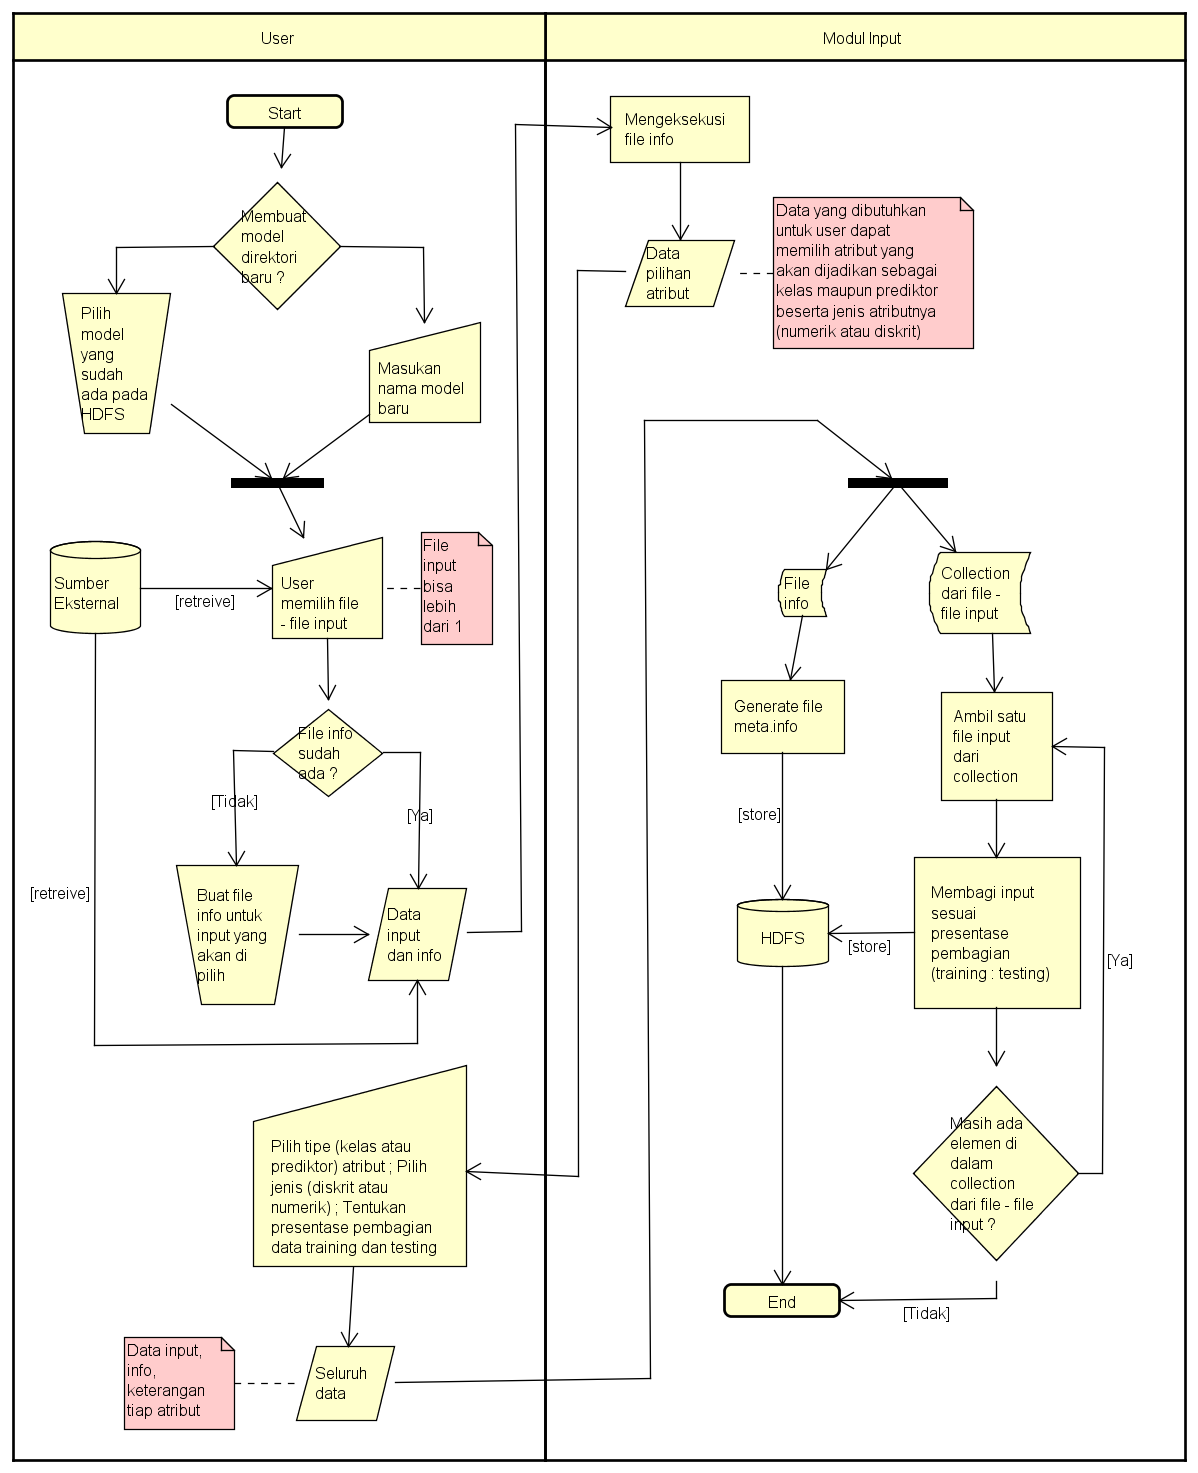
\includegraphics[scale=0.55]{Diagram/Flowchart_Input}
	\caption[Flow Chart Modul Input]{Flow Chart Modul Input}
	\label{fig:Flow Chart Modul Input}
\end{figure}

\paragraph{Pemilihan Data Masukan}
Data yang dapat digunakan pada perangkat lunak yang dibuat adalah data tidak terstruktur yang menggunakan \textit{comma-separated values}\footnote{ CSV (comma-separated values) merupakan data tabular yang berada di dalam plain text. Setiap baris dari data tersebut menyatakan sebuah record. Setiap record memiliki 1 atau lebih field yang dipisahkan oleh koma}. Data tidak terstruktur (\textit{unstructured data}) adalah data yang tidak memiliki format pasti. Data tidak terstruktur biasanya merupakan data text yang berukuran sangat besar dan format dari isi datanya juga dapat memiliki format yang bermacam - macam, seperti: tanggal ; angka ; suatu kejadian ; dsb. 
Data - data yang digunakan bisa saja berupa data pencatatan pembelian selama 3 tahun terakhir dari suatu perusahaan, data penjualan mobil dengan spesifikasi kriteria yang rinci dari suatu perusahaan mobil, dsb. Selain itu, data yang digunakan juga perlu memiliki ukuran yang cukup besar (supaya manfaat dari penggunaan framework hadoop akan lebih terlihat signifikan). Seperti pada contoh data berikut mengenai penentuan seseorang akan bermain tenis atau tidak jika diberikan beberapa fakta yang terjadi terkait faktor lingkungan dan waktu :

\begin{lstlisting}
Outlook,Temperature,Humidity,Windy,Play,Rand,Hour
Rainy,Hot,High,FALSE,No,3.5,12:00:00
Rainy,Hot,High,TRUE,No,12,14:00:00
Overcast,Hot,High,FALSE,Yes,11,,16:00:00
Sunny,Mild,High,FALSE,Yes,4,,18:00:00
Sunny,Cool,Normal,FALSE,Yes,2,09:00:00
Sunny,Cool,Normal,TRUE,No,1.9,17:00:00
Overcast,Cool,Normal,TRUE,Yes,6.4,20:00:00
Rainy,Mild,High,FALSE,No,10,07:00:00
Rainy,Cool,Normal,FALSE,Yes,9,06:00:00
\end{lstlisting}
Pada kolom pertama, ke-dua, ke-tiga, ke-empat, dan ke-lima merupakan data yang bertipe diskrit dan pada kolom ke-enam dan ke-tujuh merupakan data yang bertipe numerik. Tetapi, pada kolom ke-tujuh, perlu diberikan penanganan lebih lanjut karena data tersebut perlu dikonversi terlebih dahulu dari yang berbentuk jam ke bentuk numerik yang sederhana.

\paragraph{Kebutuhan Pra-pengolahan Data}

Pada teknik data mining, diperlukan fase pra-pengolahan data terlebih dahulu sebelum melakukan mining dengan teknik tertentu, agar data yang masuk ke dalam perangkat lunak memiliki format yang pasti. Pada skripsi kali ini, fase pra-pengolahan akan diperlukan untuk mendeteksi dan menangani terjadinya \textit{missing values}\footnote{\textit{Missing-values} merupakan keadaan dimana jumlah field pada suatu record tidak memenuhi jumlah field yang seharusnya} pada data. Pendekatan yang digunakan untuk mengatasi terjadinya \textit{missing-values} yang dapat menyebabkan analisis berjalan tidak lancar ini adalah metode \textit{listwise deletion}. \textit{Listwise deletion} merupakan salah satu metode dalam cabang ilmu statistika untuk mengatasi terjadi \textit{missing-values} dengan cara mengabaikan seluruh record - record yang memiliki \textit{missing-values} \cite{PeughMissing:2004}.

\begin{figure}[ht]
	\centering
	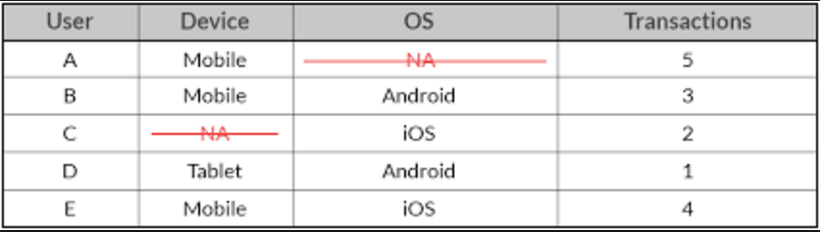
\includegraphics[scale=0.5]{GambarIO/Missing-values}
	\caption[Missing-values]{Missing-values \cite{MissingVal:2016}} 
	\label{fig:Missing-values}
\end{figure}

\subsubsection{Modul \textit{Train Naive Bayes M-R Based}}

Sebelum modul ini dijalankan, proses pada modul Input haruslah terlebih dulu selesai, karena file yang menjadi input pada modul ini merupakan hasil dari salinan file yang dijalankan pada proses dalam modul Input. Pada modul ini akan dijalankan proses train dalam pembentukan model klasifikasi naive bayes. Program \textit{training} klasifikasi naive bayes dibuat di atas framework mapreduce yang akan dijalankan pada Hadoop. Terdapat 2 pengecekan yang akan dilakukan pada modul ini, yaitu untuk menghitung atribut yang bertipe diskrit dan numerik(kontinu).\\
	Program pada modul ini akan memisahkan cara perhitungan yang digunakan dalam membangun sebuah model \textit{naive bayes classifier}. Algoritma Naive Bayes yang akan diimplementasikan pada program akan menerima input berupa dataset dan info mengenai dataset tersebut. Info yang akan diberikan meliputi atribut yang digunakan untuk melakukan pembuatan model classifier, tipe dari tiap atribut yang akan digunakan, dan atribut yang akan menjadi kelas-nya.
	
Berikut merupakan diagram \textit{flow chart} untuk modul \textit{training}:

\begin{figure}[H]
	\centering
	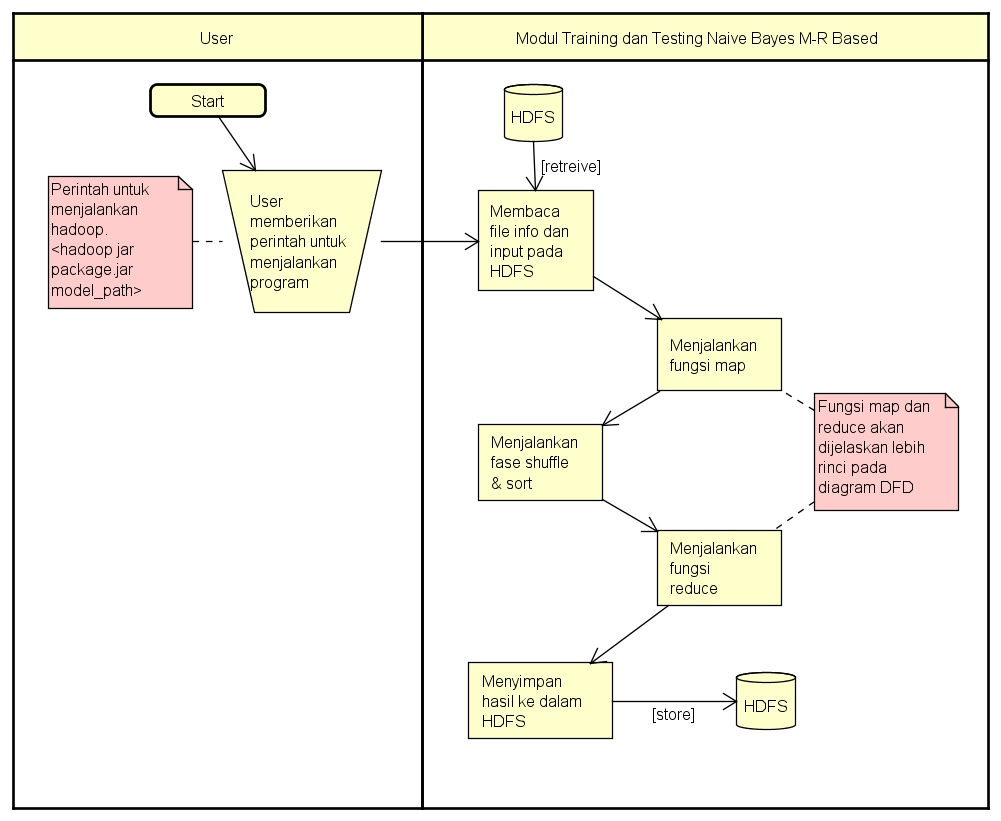
\includegraphics[scale=0.65]{Diagram/Flowchart_Training_Testing_MR}
	\caption[Flow Chart Modul Training]{Flow Chart Modul Training}
	\label{fig:Flow Chart Modul Training}
\end{figure}

Untuk proses yang berbasis \textit{MapReduce} pada modul ini perlu digambarkan menggunakan DFD, agar bisa tergambarkan lebih rinci mengenai detail proses tersebut. Berikut merupakan \textit{context diagram}\footnote{\textit{Context Diagram biasa disebut juga sebagai DFD level 0.}} dan DFD untuk proses \textit{MapReduce} pada modul \textit{training}:

\paragraph{\textit{Context Diagram} Modul \textit{Training}}
\label{par:contextdiagramTraining}

\begin{figure}[H]
	\label{DFD_0_Training}
	\centering
	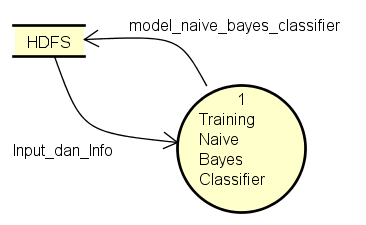
\includegraphics[scale=0.65]{Diagram/DFD_0_Training}
	\caption[\textit{Context diagram} modul Training]{\textit{Context diagram} modul Training}
	\label{fig:Context diagram modul Training}
\end{figure}

\paragraph{\textit{Data Dictionary} \textit{Context Diagram} Modul \textit{Training}}
\begin{enumerate}
	\item{Data \verb|model_naive_bayes_classifier|}
	\begin{itemize}
		\item \textit{Class Name} = [A..Z|a..z] \textcolor{red}{*}\textit{required}
		\item \textit{Class Value} = [A..Z|a..z] \textcolor{red}{*}\textit{required}
		\item \textit{Atribute Type} = [A..Z|a..z] \textcolor{red}{*}\textit{required}
		\item Frekuensi kemunculan = [0..9] \textcolor{red}{*}\textit{required}
		\item \textit{Predictor Name} = [A..Z|a..z]
		\item \textit{Predictor Value} = [A..Z|a..z]
		\item \textit{Mean} = [0..9]
		\item \textit{Sigma (standard deviation)} = [0..9]
	\end{itemize}
	Contoh data \verb|model_naive_bayes_classifier|:
	\begin{lstlisting}
	Play,Yes,2.0|CLASS
	Play,No,3.0|CLASS
	Humidity,Play,Yes ;82.5|3.5|NUMERIC
	Humidity,Play,No ;71.0|9.6|NUMERIC
	Outlook,Sunny,Play,Yes,2.0|DISCRETE
	Outlook,Sunny,Play,No,1.0|DISCRETE
	Outlook,Rainy,Play,No,2.0|DISCRETE
	\end{lstlisting}
		
	\item{Data \verb|input_dan_info|}
	\begin{itemize}
		\item Data nilai tiap field = [A..Z|a..z|0..9] \textcolor{red}{*}\textit{required}
		\item Nama - nama field = [A..Z|a..z] \textcolor{red}{*}\textit{required}
	\end{itemize}
	Contoh data \verb|input_dan_info|:
	\begin{lstlisting}
	<- Data input ->	
	Sunny,Mild,Normal,FALSE,Yes,5
	Rainy,Mild,Normal,TRUE,Yes,4.5
	Overcast,Mild,High,TRUE,Yes,3.1
	Overcast,Hot,Normal,FALSE,Yes,8.2
	Sunny,Mild,High,TRUE,No,3
	<- Data info ->
	Outlook,Temperature,Humidity,Windy,Rand
	\end{lstlisting}
\end{enumerate}


\paragraph{DFD \textit{level} 1}
\begin{figure}[H]
	\centering
	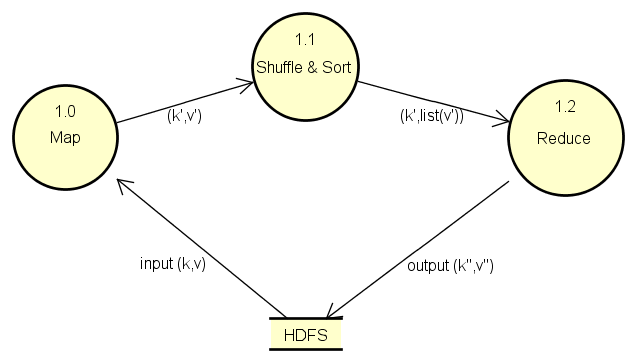
\includegraphics[scale=0.65]{Diagram/DFD_1_0_Training_Testing}
	\caption[DFD level 1 modul Training]{DFD level 1 modul Training}
	\label{fig:DFD level 1 modul Training}
\end{figure}

\paragraph{\textit{Data Dictionary} pada DFD \textit{level} 1}
\begin{enumerate}
	\item{Data \verb|input(k,v)|}
		\begin{itemize}
			\item Key: \textit{NULL}. Karena, memang pada pertama kali data diambil dari HDFS, key-nya belum terdefinisi.
			\item Value: Nilai dari tiap field yang ada = [A..Z|a..z|0..9] \textcolor{red}{*}\textit{required}
		\end{itemize}
		Contoh data \verb|input_dan_info|:
		\begin{lstlisting}
		key		value		
				Sunny,Mild,Normal,FALSE,Yes,5
				Rainy,Mild,Normal,TRUE,Yes,4.5
				Overcast,Mild,High,TRUE,Yes,3.1
				Overcast,Hot,Normal,FALSE,Yes,8.2
				Sunny,Mild,High,TRUE,No,3
		\end{lstlisting}
	\item{Data \verb|(k',v')|}
		\begin{itemize}
			\item \textit{Key} terdiri dari:
			\begin{enumerate}
				\item \textit{Class Name} = [A..Z|a..z] \textcolor{red}{*}\textit{required}
				\item \textit{Class Value} = [A..Z|a..z] \textcolor{red}{*}\textit{required}
				\item \textit{Attribute Type} = [A..Z|a..z] \textcolor{red}{*}\textit{required}
				\item \textit{Predictor Name} = [A..Z|a..z]
				\item \textit{Predictor Value} = [A..Z|a..z|0..9]
			\end{enumerate}
			\item \textit{Value} memiliki 3 jenis format yang berbeda untuk tiap jenis atribut, diantaranya adalah: 
			\begin{enumerate}
				\item Nilai dari atribut numerik dan \textit{kelas} = [0..9]
				\item Diskrit: Frekuensi kemunculan = [1] (frekuensi kemunculan untuk satu probabiltas posterior pasti bernilai 1)
			\end{enumerate}
		\end{itemize}
			Contoh data \verb|(k',v')|:
			\begin{lstlisting}
			key									value		
			|_class|Play,Yes					1
			|disc|Humidity,High,Play,No			1
			|cont|Rand,Play,Yes					34.2
			\end{lstlisting}

	\item{Data \verb|(k',list(v'))|}
	\begin{itemize}
		\item Format data untuk variabel \textit{key}, masih sama dengan format variabel \textit{key} pada data \verb|(k,v)|.
		\item Untuk variabel \textit{value} juga demikian, tetapi tipe-nya berubah menjadi list.
	\end{itemize}
	Contoh data \verb|(k',list(v'))|
	\begin{lstlisting}
		key										list_of_value		
			|_class|Play,Yes					[1,1,1,1]
			|disc|Humidity,High,Play,No			[1,1]
			|cont|Rand,Play,Yes					[34.2,23.3,15.0]
	\end{lstlisting}
	\item{Data \verb|input(k",v")|}
	\begin{itemize}
		\item Format data untuk variabel \textit{key}, sama dengan format variabel \textit{key} pada data \verb|(k,v)|, tetapi untuk atribut yang bertipe diskrit dan kelas, ditambahkan dengan jumlah frekuensi kemunculan pada tiap probabilitas posterior yang muncul.
		\item Format atribut \textit{value} untuk tiap jenis:
		\begin{enumerate}
			\item{Diskrit}: \textit{NULL}
			\item{Kelas}: \textit{NULL}
			\item{Numerik}: \textit{mean}, \textit{sigma}, dan tipe atribut(numerik) = [A..Z|a..z|0..9]
		\end{enumerate}
	\end{itemize}

	\begin{lstlisting}
	key											value
	Play,Yes,5.0|CLASS							(empty-string)
	Rand,Play,No								;6.85|4.247|NUMERIC
	Humidity,High,Play,No,3.0|DISCRETE			(empty-string)
	\end{lstlisting}
	
\end{enumerate}

\paragraph{DFD \textit{level} 2: pada proses 1.0}
\begin{figure}[H]
	\centering
	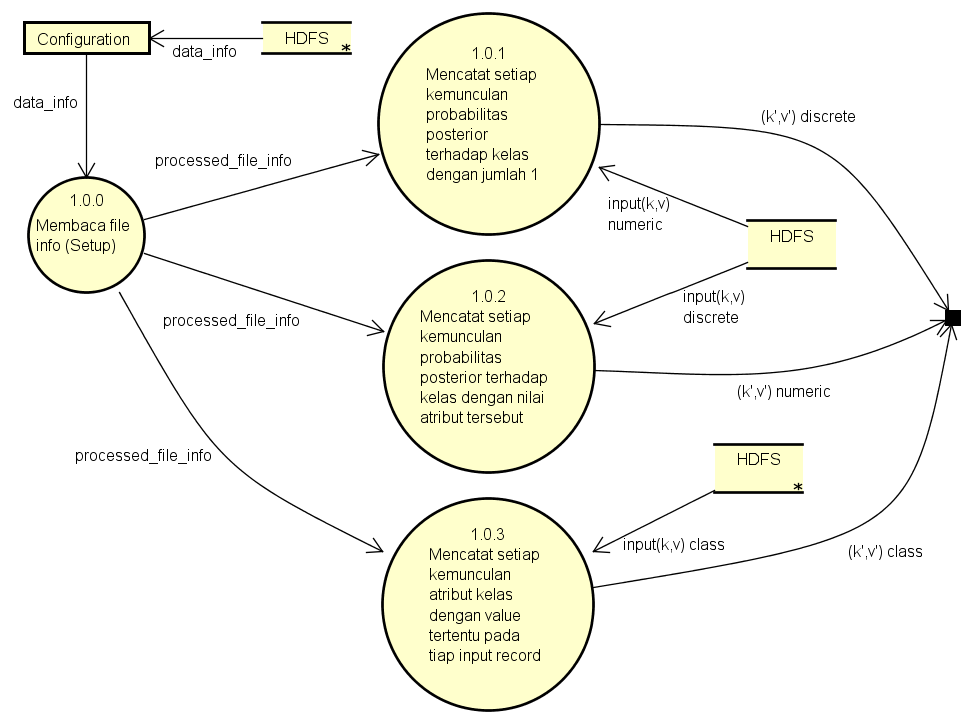
\includegraphics[scale=0.5]{Diagram/DFD_1_1_Training_Map}
	\caption[DFD level 2: proses 1.0]{DFD level 2: proses 1.0}
	\label{fig:DFD level 2: proses 1.0}
\end{figure}

\paragraph{\textit{Data Dictionary} pada DFD \textit{level} 2: proses 1.0}
\begin{enumerate}
	\item{Data \verb|data_info|}
		\begin{itemize}
			\item Nama field atribut kelas yang dipakai pada \textit{training} = [A..Z|a..z]
			\item Nama field atribut prediktor yang dipakai pada \textit{training} = [A..Z|a..z]
			\item Nomor indeks dari atribut kelas = [0..9]
			\item Nomor indeks dari atribut prediktor = [0..9]
			\item Tipe jenis atribut prediktor = [A..Z|a..z]
			\item Jumlah field yang ada pada data \textit{input} = [0..9]
		\end{itemize}
		 \textcolor{red}{*}Setiap atribut pada prediktor akan dipisahkan menggunakan karakter titik-koma\textit{(;)}.\\
	Contoh data \verb|data_info|
	\begin{lstlisting}
	<- prediktor ->
	Outlook,0,DISCRETE;Temperature,1,DISCRETE;Windy,3,DISCRETE;Rand,5,NUMERICAL
	<- kelas ->
	Play,4
	<- jumlah field ->
	6
	\end{lstlisting}
	
	\item{Data \verb|processed_file_info|}
	Isi dari data \verb|processed_file_info| sama dengan data \verb|data_info|. Tetapi, format dan jenis tipe datanya dibedakan sedikit.
	Contoh data \verb|data_info|
	\begin{lstlisting}
	<- prediktor ->
	[
		{Outlook,0,DISCRETE},
		{Temperature,1,DISCRETE},
		{Windy,3,DISCRETE},
		{Rand,5,NUMERICAL},
	]
	<- kelas ->
	[
		{Play,4},
	]
	<- jumlah field ->
	6
	\end{lstlisting}	
	
	\item{Data \verb|input(k,v)numeric|}\\
	Format pada data ini akan memiliki format sama dengan data pada \verb|data_input|. Pengecekan akan dilakukan oleh sistem yang dibuat untuk mengenali tipe atribut dari tiap field yang akan diperiksanya.	
	
	\item{Data \verb|input(k,v)discrete|}
	Format pada data ini akan memiliki format sama dengan data pada \verb|data_input|. Pengecekan akan dilakukan oleh sistem yang dibuat untuk mengenali tipe atribut dari tiap field yang akan diperiksanya.

	\item{Data \verb|(k',v')class|}
	\begin{itemize}
		\item \textit{Key} terdiri dari:
		\begin{enumerate}
			\item \textit{Class Name} = [A..Z|a..z] \textit{\textcolor{red}{*}required}
			\item \textit{Class Value} = [A..Z|a..z] \textit{\textcolor{red}{*}required}
		\end{enumerate}
		\item \textit{Value} terdiri dari:
		\begin{enumerate}
			\item Frekuensi kemunculan atribut kelas tersebut = [1](bernilai selalu 1)
		\end{enumerate}
	\end{itemize}
	
	\item{Data \verb|(k',v')discrete|}
	\begin{itemize}
		\item \textit{Key} terdiri dari:
		\begin{enumerate}
			\item \textit{Class Name} = [A..Z|a..z] \textit{\textcolor{red}{*}required}
			\item \textit{Class Value} = [A..Z|a..z] \textit{\textcolor{red}{*}required}
			\item \textit{Attribute Type} = [A..Z|a..z] \textit{\textcolor{red}{*}required}
			\item \textit{Predictor Name} = [A..Z|a..z] \textcolor{red}{*}\textit{required}
			\item \textit{Predictor Value} = [A..Z|a..z|0..9] \textcolor{red}{*}\textit{required}
		\end{enumerate}
		\item \textit{Value} terdiri dari:
		\begin{enumerate}
			\item Frekuensi kemunculan dari probabilitas posterior = [1] (bernilai selalu 1).
		\end{enumerate}
	\end{itemize}

	\item{Data \verb|(k',v')numeric|}
	\begin{itemize}
		\item \textit{Key} terdiri dari:
		\begin{enumerate}
			\item \textit{Class Name} = [A..Z|a..z] \textit{\textcolor{red}{*}required}
			\item \textit{Class Value} = [A..Z|a..z] \textit{\textcolor{red}{*}required}
			\item \textit{Attribute Type} = [A..Z|a..z] \textit{\textcolor{red}{*}required}
			\item \textit{Predictor Name} = [A..Z|a..z] \textcolor{red}{*}\textit{required}
		\end{enumerate}
		\item \textit{Value} terdiri dari:
		\begin{enumerate}
			\item Nilai dari atribut numerik tersebut = [0..9]
		\end{enumerate}
	\end{itemize}

\end{enumerate}

\paragraph{P-Spec (\textit{Process Specification}) pada DFD \textit{level} 2: pada proses 1.0}
\begin{figure}[H]
	\centering
	\includegraphics[scale=0.6]{PSpec/P-Spec_dfd_1_0_0_train}
	\caption[P-Spec proses 1.0.0]{P-Spec training map: pada proses 1.0.0}
	\label{fig:P-Spec training: pada proses 1.0.0}
\end{figure}

\begin{figure}[H]
	\centering
	\includegraphics[scale=0.6]{PSpec/P-Spec_dfd_1_0_1_train}
	\caption[P-Spec proses 1.0.1]{P-Spec training map: pada proses 1.0.1}
	\label{fig:P-Spec training: pada proses 1.0.1}
\end{figure}

\begin{figure}[H]
	\centering
	\includegraphics[scale=0.6]{PSpec/P-Spec_dfd_1_0_2_train}
	\caption[P-Spec proses 1.0.2]{P-Spec training map: pada proses 1.0.2}
	\label{fig:P-Spec training: pada proses 1.0.2}
\end{figure}

\begin{figure}[H]
	\centering
	\includegraphics[scale=0.6]{PSpec/P-Spec_dfd_1_0_3_train}
	\caption[P-Spec proses 1.0.3]{P-Spec training map: pada proses 1.0.3}
	\label{fig:P-Spec training: pada proses 1.0.3}
\end{figure}

\paragraph{DFD \textit{level} 2: pada proses 1.1}
\begin{figure}[H]
	\centering
	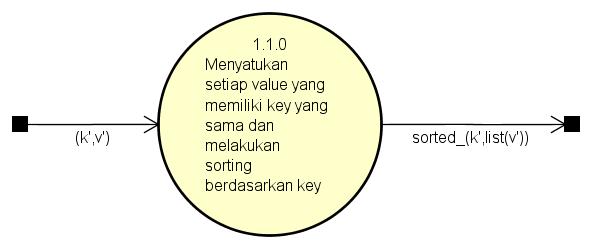
\includegraphics[scale=0.65]{Diagram/DFD_1_2_Training_Test_SS}
	\caption[DFD level 2: proses 1.1]{DFD level 2: proses 1.1}
	\label{fig:DFD level 2: proses 1.1}
\end{figure}

\paragraph{\textit{Data Dictionary} pada DFD \textit{level} 2: proses 1.1}
\begin{enumerate}
	\item{Data \verb|(k,v)|}
	\begin{itemize}
		\item \textit{Key} terdiri dari:
		\begin{enumerate}
			\item \textit{Class Name} = [A..Z|a..z] \textit{\textcolor{red}{*}required}
			\item \textit{Class Value} = [A..Z|a..z] \textit{\textcolor{red}{*}required}
			\item \textit{Attribute Type} = [A..Z|a..z] \textit{\textcolor{red}{*}required}
			\item \textit{Predictor Name} = [A..Z|a..z]
			\item \textit{Predictor Value} = [A..Z|a..z|0..9]
		\end{enumerate}
		\item \textit{Value} terdiri dari:
		\begin{enumerate}
			\item Frekuensi kemunculan dari atribut kelas = [1]
			\item Frekuensi kemunculan dari atribut prediktor = [1]
			\item Nilai dari atribut numerik = [0..9]
		\end{enumerate}
	\end{itemize}
	Contoh data \verb|(k,v)|
	\begin{lstlisting}
	key								value
	|_class|Play,Yes				1
	|cont|Rand,Play,Yes				32.5
	|disc|Humidity,High,Play,No		1
	\end{lstlisting}
	
	\item{Data \verb|sorted_(k',list(v'))|}
	Format dari variabel \textit{key} dan \textit{value} sama dengan data pada \verb|(k,v)|. Hanya tipe pada variabel \textit{value} diubah menjadi list.\\
	Contoh data \verb|sorted_(k',list(v'))|
	\begin{lstlisting}
	key								list_of_value
	|_class|Play,Yes				[1,1,1,1]
	|cont|Rand,Play,Yes				[32.5,24.5]
	|disc|Humidity,High,Play,No		[1,1]
	\end{lstlisting}
\end{enumerate}

\paragraph{P-Spec (\textit{Process Specification}) pada proses 1.1}
\begin{figure}[H]
	\centering
	\includegraphics[scale=0.6]{PSpec/P-Spec_dfd_1_1_0_train_testing}
	\caption[P-Spec training reduce: pada proses 1.1.0]{P-Spec training shuffle sort: pada proses 1.1.0}
	\label{fig:P-Spec training shuffle sort: pada proses 1.1.0}
\end{figure}


\paragraph{DFD \textit{level} 2: pada proses 1.2}
\begin{figure}[H]
	\centering
	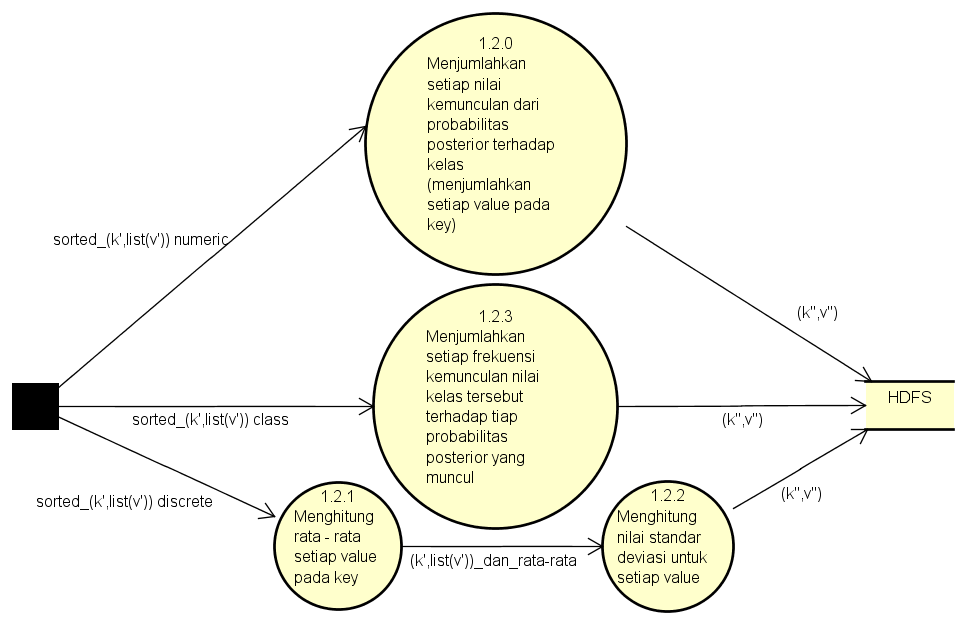
\includegraphics[scale=0.6]{Diagram/DFD_1_3_Training_Red}
	\caption[DFD level 2: proses 1.2]{DFD level 2: proses 1.2}
	\label{fig:DFD level 2: proses 1.2}
\end{figure}

\paragraph{\textit{Data Dictionary} pada DFD \textit{level} 2: proses 1.2}
\begin{enumerate}
	\item{Data \verb|sorted_(k',list(v'))numeric|}
	\begin{itemize}
		\item \textit{Key} terdiri dari:
		\begin{enumerate}
			\item \textit{Class Name} = [A..Z|a..z] \textit{\textcolor{red}{*}required}
			\item \textit{Class Value} = [A..Z|a..z] \textit{\textcolor{red}{*}required}
			\item \textit{Attribute Type} = [A..Z|a..z] \textit{\textcolor{red}{*}required}
			\item \textit{Predictor Name} = [A..Z|a..z] \textit{\textcolor{red}{*}required}
		\end{enumerate}
		\item \textit{Value} terdiri dari:
		\begin{enumerate}
			\item Nilai dari atribut numerik itu sendiri = [0..9]
		\end{enumerate}
	\end{itemize}
	Contoh data \verb|sorted_(k',list(v'))numeric|
	\begin{lstlisting}
		key							list_of_value
		|cont|Rand,Play,Yes			[32.5,25.3]
		|cont|Rand,Play,No			[40.21,54.3]
	\end{lstlisting}
	
	\item{Data \verb|sorted_(k',list(v'))discrete|}
	\begin{itemize}
		\item \textit{Key} terdiri dari:
		\begin{enumerate}
			\item \textit{Class Name} = [A..Z|a..z] \textit{\textcolor{red}{*}required}
			\item \textit{Class Value} = [A..Z|a..z] \textit{\textcolor{red}{*}required}
			\item \textit{Attribute Type} = [A..Z|a..z] \textit{\textcolor{red}{*}required}
			\item \textit{Predictor Name} = [A..Z|a..z] \textit{\textcolor{red}{*}required}
			\item \textit{Predictor Value} = [A..Z|a..z] \textit{\textcolor{red}{*}required}
		\end{enumerate}
		\item \textit{Value} terdiri dari:
		\begin{enumerate}
			\item Frekuensi kemunculan = [1]
		\end{enumerate}
	\end{itemize}
	Contoh data \verb|sorted_(k',list(v'))discrete|
	\begin{lstlisting}
		key									list_of_value
		|disc|Humidity,High,Play,No			[32.5,25.3]
		|disc|Humidity,High,Play,Yes		[40.21,54.3]
	\end{lstlisting}
	
	\item{Data \verb|sorted_(k',list(v'))class|}
	\begin{itemize}
		\item \textit{Key} terdiri dari:
		\begin{enumerate}
			\item \textit{Class Name} = [A..Z|a..z] \textit{\textcolor{red}{*}required}
			\item \textit{Class Value} = [A..Z|a..z] \textit{\textcolor{red}{*}required}
			\item \textit{Attribute Type} = [A..Z|a..z] \textit{\textcolor{red}{*}required}
		\end{enumerate}
		\item \textit{Value} terdiri dari:
		\begin{enumerate}
			\item Frekuensi kemunculan = [1]
		\end{enumerate}
	\end{itemize}
	Contoh data \verb|sorted_(k',list(v'))class|
	\begin{lstlisting}
		key						list_of_value
		|_class|Play,No			[1,1,1,1]
		|_class|Play,Yes		[1,1,1,1,1,1,1]
	\end{lstlisting}

	\item{Data \verb|sorted_(k',list(v'))_dan_rata-rata|}
	\begin{itemize}
		\item \textit{Key} terdiri dari:
		\begin{enumerate}
			\item \textit{Class Name} = [A..Z|a..z] \textit{\textcolor{red}{*}required}
			\item \textit{Class Value} = [A..Z|a..z] \textit{\textcolor{red}{*}required}
			\item \textit{Attribute Type} = [A..Z|a..z] \textit{\textcolor{red}{*}required}
		\end{enumerate}
		\item \textit{Value} terdiri dari:
		\begin{enumerate}
			\item Frekuensi kemunculan = [1]
		\end{enumerate}
		\item Rata - rata dari seluruh \textit{list of value} tersebut = [0..9]
	\end{itemize}
	Contoh data \verb|sorted_(k',list(v'))_dan_rata-rata|
	\begin{lstlisting}
		key									list_of_value	rata-rata
		|cont|Humidity,High,Play,No			[32.5,25.3]		28.9	
		|cont|Humidity,High,Play,Yes		[40.21,54.3]	47.255
	\end{lstlisting}

	\item{Data \verb|(k",v")|}
	\begin{itemize}
		\item \textit{Key} terdiri dari:
		\begin{enumerate}
			\item \textit{Class Name} = [A..Z|a..z] \textit{\textcolor{red}{*}required}
			\item \textit{Class Value} = [A..Z|a..z] \textit{\textcolor{red}{*}required}
			\item \textit{Attribute Type} = [A..Z|a..z]	\textit{\textcolor{red}{*}required}	
			\item \textit{Predictor Name} = [A..Z|a..z]	
			\item \textit{Predictor Value} = [A..Z|a..z]
			\item Frekuensi kemunculan untuk atribut diskrit/kelas = [0..9]
		\end{enumerate}
				
		\item \textit{Value} untuk atribut numerik terdiri dari:
		\begin{enumerate}
			\item \textit{Predictor Value} = [0..9] 
			\item \textit{Attribute Type} = [A..Z|a..z] 			
			\item \textit{Mean} = [0..9]
			\item \textit{Sigma} = [0..9]
		\end{enumerate}
	\end{itemize}
	Contoh data \verb|(k",v")|
	\begin{lstlisting}
	key									value
	Play,No,3.0|CLASS					(empty-string)
	Humidity,Play,Yes 					;82.5|3.5|NUMERIC
	Outlook,Sunny,Play,Yes,2.0|DISCRETE	(empty-string)
	Outlook,Rainy,Play,No,2.0|DISCRETE	(empty-string)
	\end{lstlisting}


\end{enumerate}


\paragraph{P-Spec (\textit{Process Specification}) pada proses 1.2}

\begin{figure}[H]
	\centering
	\includegraphics[scale=0.6]{PSpec/P-Spec_dfd_1_2_0_train}
	\caption[P-Spec training reduce: pada proses 1.2.0]{P-Spec training reduce: pada proses 1.2.0}
	\label{fig:P-Spec training reduce: pada proses 1.2.0}
\end{figure}

\begin{figure}[H]
	\centering
	\includegraphics[scale=0.6]{PSpec/P-Spec_dfd_1_2_1_train}
	\caption[P-Spec training reduce: pada proses 1.2.1]{P-Spec training reduce: pada proses 1.2.1}
	\label{fig:P-Spec training reduce: pada proses 1.2.1}
\end{figure}

\begin{figure}[H]
	\centering
	\includegraphics[scale=0.6]{PSpec/P-Spec_dfd_1_2_2_train}
	\caption[P-Spec training reduce: pada proses 1.2.2]{P-Spec training reduce: pada proses 1.2.2}
	\label{fig:P-Spec training reduce: pada proses 1.2.2}
\end{figure}

\begin{figure}[H]
	\centering
	\includegraphics[scale=0.6]{PSpec/P-Spec_dfd_1_2_3_train}
	\caption[P-Spec training: pada proses 1.2.3]{P-Spec training reduce: pada proses 1.2.3}
	\label{fig:P-Spec training reduce: pada proses 1.2.3}
\end{figure}


\subsubsection{Modul \textit{Testing Naive Bayes M-R Based}}

Pada modul ini, program akan memanfaatkan model klasifikasi naive bayes yang telah dibuat sebelumnya untuk melakukan klasifikasi pada data testing yang telah ada sebelumnya di HDFS (pada modul input) dan memberikan laporan analisis mengenai tingkat akurasi dan tingkat error yang dimiliki oleh model terhadap data tersebut. 

Berikut merupakan diagram \textit{flow chart} untuk modul \textit{testing}:

\begin{figure}[H]
	\centering
	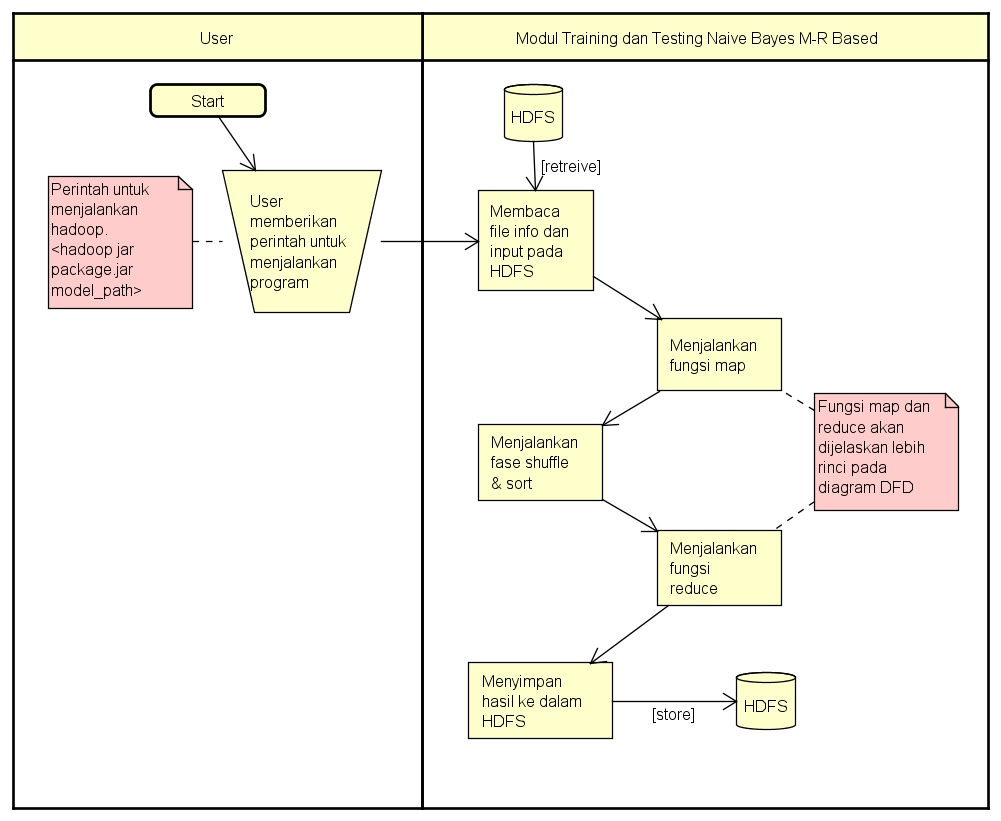
\includegraphics[scale=0.6]{Diagram/Flowchart_Training_Testing_MR}
	\caption[Flow Chart Modul Testing]{Flow Chart Modul Testing}
	\label{fig:Flow Chart Modul Testing}
\end{figure}

Sama seperti pada modul \textit{training}, untuk proses yang berbasis \textit{MapReduce} pada modul ini juga perlu digambarkan menggunakan DFD, agar bisa tergambarkan lebih rinci mengenai detail proses tersebut. Berikut merupakan \textit{context diagram}\footnote{\textit{Context Diagram biasa disebut juga sebagai DFD level 0.}} dan DFD untuk proses \textit{MapReduce} pada modul \textit{testing}:

\paragraph{\textit{Context Diagram} Modul \textit{Testing}}
\label{par:contextdiagramTesting}
\begin{figure}[H]
	\centering
	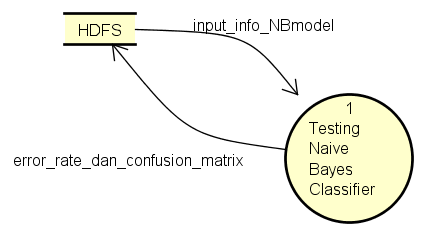
\includegraphics[scale=0.65]{Diagram/DFD_0_Testing}
	\caption[\textit{Context diagram} modul Testing]{\textit{Context diagram} modul Testing}
	\label{fig:Context diagram modul Testing}
\end{figure}

\paragraph{\textit{Data Dictionary} \textit{Context Diagram} Modul \textit{Testing}}
\begin{enumerate}
	\item{Data \verb|input_info_NBmodel|} terdiri dari input dan NBC (\textit{Naive Bayes Classifier}) model.
	\begin{itemize}
		\item \textit{Input} terdiri dari: 
		\begin{enumerate}
			\item Nilai dari atribut kelas pada input = [A..Z|a..z]
			\item Nilai dari atribut prediktor bertipe diskrit pada input = [A..Z|a..z]
			\item Nilai dari atribut prediktor bertipe numerik pada input = [0..9]
		\end{enumerate}						
		
		\item NBC model terdiri dari:
		\begin{enumerate}
			\item \textit{Class Name} = [A..Z|a..z|]
			\item \textit{Class Value} = [A..Z|a..z|] 
			\item \textit{Attribute Type} = [A..Z|a..z|] 
			\item \textit{Predictor Name} = [A..Z|a..z|]
			\item \textit{Predictor Value} = [A..Z|a..z|]
			\item Frekuensi kemunculan untuk tiap atribut kelas	= [A..Z|a..z|0..9]
			\item Frekuensi kemunculan untuk tiap atribut prediktor diskrit	= [A..Z|a..z|0..9]
			\item Nilai mean dari atribut prediktor numerik = [0..9]
			\item Nilai sigma/standard-deviasi dari atribut prediktor numerik = [0..9]
		\end{enumerate}		
		
	\end{itemize}
	Contoh data \verb|input_info_NBmodel|
	\begin{lstlisting}
	<- input ->
	Sunny,Mild,Normal,FALSE,Yes,5
	Rainy,Mild,Normal,TRUE,Yes,4.5
	Overcast,Mild,High,TRUE,Yes,3.1
	<- NBmodel ->
	Play,Yes,2.0|CLASS
	Play,No,3.0|CLASS
	Humidity,Play,Yes ;82.5|3.5|NUMERIC
	Humidity,Play,No ;71.0|9.6|NUMERIC
	Outlook,Sunny,Play,Yes,2.0|DISCRETE
	Outlook,Sunny,Play,No,1.0|DISCRETE
	Outlook,Rainy,Play,No,2.0|DISCRETE
	\end{lstlisting}
		
	\item{Data \verb|error_rate_dan_confusion_matrix|}
	\begin{itemize}
		\item Nama kelas = [A..Z|a..z]
		\item \textit{Confusion Matrix} untuk tiap kelas = matrix $n*m$
		\item \textit{Error rate} untuk $Accuracy$ untuk tiap kelas = [0..9]
		\item \textit{Error rate} untuk $Recall$ untuk tiap \textit{class value} = [0..9]
		\item \textit{Error rate} untuk $Precision$ untuk tiap \textit{class value} = [0..9]
		\item \textit{Error rate} untuk $F-Measure$ untuk tiap \textit{class value} = [0..9]
	\end{itemize}
	\begin{lstlisting}
	@play
	####
	|		|	no	| yes	|
	| no	|	3	| 0		|
	| yes	|	0	| 2		|
	####
	Accuracy: 5/5 = 1.0
	*For Value = no
	Precision: -> 3 / 3 + 0 = 1.0
	Recall: -> 3 / 3 + 0 = 1.0 
	*For Value = yes
	Precision: -> 2 / 2 + 0 = 1.0
	Recall: -> 2 / 2 + 0 = 1.0
	F-Measure -> 0.8
	\end{lstlisting}
	
\end{enumerate}


\paragraph{DFD \textit{level} 1}
\begin{figure}[H]
	\centering
	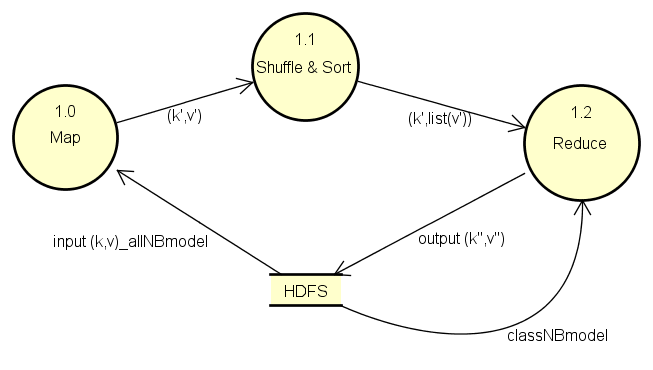
\includegraphics[scale=0.65]{Diagram/DFD_1_0_Testing_rdmodel}
	\caption[DFD level 1 modul Testing]{DFD level 1 modul Testing}
	\label{fig:DFD level 1 modul Testing}
\end{figure}

\paragraph{\textit{Data Dictionary} pada DFD \textit{level} 1}
\begin{enumerate}
	\item{Data \verb|input(k,v)_allNBmodel|}
	\begin{itemize}
		\item \textit{Key} pada \verb|input(k,v)| = \textit{NULL} (karena memang pada awal proses \textit{mapreduce} key pada input belum terdefinisi)

		\item \textit{Value} pada \verb|input(k,v)| terdiri dari:
		\begin{enumerate}
			\item Nilai tiap atribut prediktor diskrit pada input = [A..Z|a..z|]
			\item Nilai tiap atribut prediktor numerik pada input = [0..9]
			\item Nilai tiap atribut kelas pada input = [A..Z|a..z]
		\end{enumerate}

		\item \textit{allNBmodel} yang merupakan model dari NBC memiliki format sama dengan NBC model yang terdapat pada data \verb|input_info_NBmodel|.
		
	\end{itemize}
	
	\item{Data \verb|(k',v')|}
	\begin{itemize}
		\item \textit{Key} yang merupakan nama atribut kelas = [A..Z|a..z]
		\item \textit{Value} terdiri dari:
		\begin{enumerate}
			\item \textit{Class Name} = [A..Z|a..z]
			\item \textit{Class Value Predicted} = [A..Z|a..z]
			\item \textit{Class Value Actual} = [A..Z|a..z]
			\item \textit{Percentage} = [0..9]
		\end{enumerate}
	\end{itemize}
	Contoh data \verb|(k',v')|
	\begin{lstlisting}
	key			value
	Play		Play|predicted=Yes|percentage=67.5%|actual=Yes
	Play		Play|predicted=Yes|percentage=51.1%|actual=No
	Play		Play|predicted=No|percentage=96.32%|actual=No	
	\end{lstlisting}

	\item{Data \verb|(k',list(v'))|}\\
	format key dan value pada data ini sama dengan data \verb|(k',v')|. Hanya saja, untuk variabel \textit{value}-nya dijadikan sebuah list untuk setiap nama variabel \textit{key} yang sama.\\
	Contoh data \verb|(k',list(v'))|
	\begin{lstlisting}
	key			list_of_value
	Play		[
					{Play|predicted=Yes|percentage=67.5%|actual=Yes},
					{Play|predicted=Yes|percentage=51.1%|actual=No},
					{Play|predicted=No|percentage=96.32%|actual=No},
				]
	\end{lstlisting}

	\item{Data \verb|output(k",v")|}
	\begin{itemize}
		\item \textit{Key} terdiri dari:
		\begin{enumerate}
			\item \textit{Class Name} = [A..Z|a..z]
			\item \textit{Confusion Matrix} untuk tiap kelas = matrix $m*n$
		\end{enumerate}
		
		\item \textit{Value} terdiri dari:
		\begin{enumerate}
			\item \textit{Error rate} untuk $Accuracy$ untuk tiap kelas = [0..9]
			\item \textit{Error rate} untuk $Recall$ untuk tiap \textit{class value} = [0..9]
			\item \textit{Error rate} untuk $Precision$ untuk tiap \textit{class value} = [0..9]
			\item \textit{Error rate} untuk $F-Measure$ untuk tiap \textit{class value} = [0..9]
		\end{enumerate}
	\end{itemize}
	Contoh data \verb|output(k",v")|
	\begin{lstlisting}
	<- Key ->
	@play
	####
	|		|	no	| yes	|
	| no	|	3	| 0		|
	| yes	|	0	| 2		|
	####
	<- Value ->
	Accuracy: 5/5 = 1.0
	*For Value = no
	Precision: -> 3 / 3 + 0 = 1.0
	Recall: -> 3 / 3 + 0 = 1.0 
	*For Value = yes
	Precision: -> 2 / 2 + 0 = 1.0
	Recall: -> 2 / 2 + 0 = 1.0
	F-Measure -> 0.8
	\end{lstlisting}

	\item{Data \verb|classNBmodel|} yang merupakan model dari NBC memiliki format hampir sama dengan NBC model yang terdapat pada data \verb|input_info_NBmodel|. Bedanya, data ini hanya mengambil model yang bertipe atribut kelas saja untuk digunakan dalam menghitung \textit{confusion matrix}.\\
	Contoh data \verb|classNBmodel|: 
	\begin{lstlisting}
	Play,Yes,2.0|CLASS
	Play,No,3.0|CLASS
	\end{lstlisting}

\end{enumerate}


\paragraph{DFD \textit{level} 2: pada proses 1.0}
\begin{figure}[H]
	\centering
	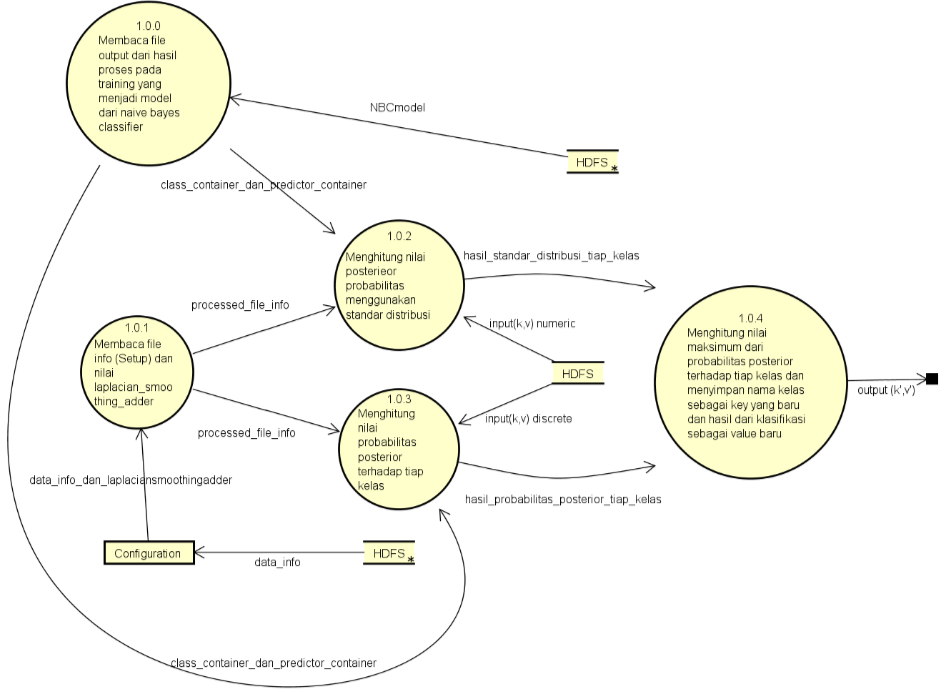
\includegraphics[scale=0.7]{Diagram/DFD_1_1_Testing_Map}
	\caption[DFD level 2: proses 1.0]{DFD level 2: proses 1.0}
	\label{fig:DFD level 2: proses 1.0}
\end{figure}

\paragraph{P-Spec (\textit{Process Specification}) pada proses 1.0}
\begin{enumerate}
	\item{Data \verb|NBCmodel|}
	yang merupakan model dari NBC memiliki format sama dengan NBC model yang terdapat pada data \verb|input_info_NBmodel| di \textit{context diagram}.
	
	\item{Data \verb|class_contanier_dan_predictor_container|}
	\begin{itemize}
		\item \textit{Class Name} = [A..Z|a..z]
		\item \textit{Class Value} = [A..Z|a..z]
		\item \textit{Predictor Name} = [A..Z|a..z]
		\item \textit{Predictor Value} = [A..Z|a..z|0..9]
		\item \textit{Attribute Type} = [A..Z|a..z]
		\item \textit{Mean} = [0..9]
		\item \textit{Sigma} = [0..9]
	\end{itemize}

	\item{Data \verb|data_info|}
	\begin{itemize}
		\item Nama tiap field = [A..Z|a..z]
		\item Nomor index tiap field = [0..9]
		\item Tipe tiap field = [A..Z|a..z]
	\end{itemize}

	\item{Data \verb|data_info_dan_laplaciansmoothingadder|} \\
	Data ini merupakan data yang sama pada data \verb|data_info|, tetapi ditambahkan nilai \textit{laplaciansmoothingadder} sebagai counter untuk penambahan tiap frekuensi probabilitas posterior untuk menghindari terjadinya permasalahan \textit{zero-frequency}.
	
	\item{Data \verb|processed_file_info|}
	Data ini merupakan data yang terdapat pada data \verb|data_info_dan_laplaciansmoothingadder|, hanya saja formatnya dibuat untuk memudahkan perangkat lunak yang nantinya dibuat membaca file info tersebut.

	\item{Data \verb|input(k,v)numeric|}
	\begin{itemize}
		\item \textit{Key} pada \verb|input(k,v)numeric| = \textit{NULL} (karena memang pada awal proses \textit{mapreduce} key pada input belum terdefinisi)

		\item \textit{Value} pada \verb|input(k,v)| terdiri dari:
		\begin{enumerate}
			\item Nilai tiap atribut prediktor numerik pada input = [0..9]
			\item Nilai tiap atribut kelas pada input = [A..Z|a..z]
		\end{enumerate}
		
	\end{itemize}

	\item{Data \verb|input(k,v)discrete|}
	\begin{itemize}
		\item \textit{Key} pada \verb|input(k,v)discrete| = \textit{NULL} (karena memang pada awal proses \textit{mapreduce} key pada input belum terdefinisi)

		\item \textit{Value} pada \verb|input(k,v)| terdiri dari:
		\begin{enumerate}
			\item Nilai tiap atribut prediktor diskrit pada input = [A..Z|a..z]
			\item Nilai tiap atribut kelas pada input = [A..Z|a..z]
		\end{enumerate}
		
	\end{itemize}

	\item{Data \verb|hasil_standar_distribusi_tiap_kelas|} merupakan nilai dari standard distribusi untuk probabilitas posterior tiap atribut numerik terhadap tiap kelas yang ada.
	\begin{itemize}
		\item \textit{Class Name} = [A..Z|a..z]
		\item \textit{Class Value} = [A..Z|a..z]
		\item \textit{Predictor Name} = [A..Z|a..z]
		\item \textit{Attribute Type} = [A..Z|a..z]
		\item Nilai standar distribusi = [0..9]
	\end{itemize}
	

	\item{Data \verb|hasil_probabilitas_posterior_tiap_kelas|}
	merupakan nilai hasil dari probabilitas posterior dari tiap atribut pada tiap atribut kelas yang ada.
	\begin{itemize}
		\item \textit{Class Name} = [A..Z|a..z]
		\item \textit{Class Value} = [A..Z|a..z]
		\item \textit{Predictor Name} = [A..Z|a..z]
		\item \textit{Predictor Value} = [A..Z|a..z]
		\item \textit{Attribute Type} = [A..Z|a..z]
		\item Hasil nilai probabilitas posterior dari tiap atribut prediktor terhadap tiap kelas = [0..9]
	\end{itemize}

	\item{Data \verb|output(k',v')|}
	\begin{itemize}
		\item \textit{Key} merupakan nama atribut kelas = [A..Z|a..z]
		
		\item \textit{Value} terdiri dari:
		\begin{enumerate}
			\item \textit{Class Name} = [A..Z|a..z]
			\item \textit{Class Value Predicted} = [A..Z|a..z]
			\item \textit{Class Actual} = [A..Z|a..z]
			\item \textit{Percentage} = [0..9]
		\end{enumerate}
		
	\end{itemize}
	Contoh data \verb|output(k',v')|:
	\begin{lstlisting}
	key			value
	Play		Play|predicted=Yes|percentage=67.5%|actual=Yes
	Play		Play|predicted=Yes|percentage=51.1%|actual=No
	Play		Play|predicted=No|percentage=96.32%|actual=No	
	\end{lstlisting}
	
\end{enumerate}


\begin{figure}[H]
	\centering
	\includegraphics[scale=0.65]{PSpec/P-Spec_dfd_1_0_9_test}
	\caption[P-Spec training reduce: pada proses 1.0.0]{P-Spec training reduce: pada proses 1.0.0}
	\label{fig:P-Spec training reduce: pada proses 1.0.0}
\end{figure}

\begin{figure}[H]
	\centering
	\includegraphics[scale=0.65]{PSpec/P-Spec_dfd_1_0_0_test}
	\caption[P-Spec training reduce: pada proses 1.0.1]{P-Spec training reduce: pada proses 1.0.1}
	\label{fig:P-Spec training reduce: pada proses 1.0.1}
\end{figure}

\begin{figure}[H]
	\centering
	\includegraphics[scale=0.65]{PSpec/P-Spec_dfd_1_0_1_test}
	\caption[P-Spec training reduce: pada proses 1.0.2]{P-Spec training reduce: pada proses 1.0.2}
	\label{fig:P-Spec training reduce: pada proses 1.0.2}
\end{figure}

\begin{figure}[H]
	\centering
	\includegraphics[scale=0.65]{PSpec/P-Spec_dfd_1_0_2_test}
	\caption[P-Spec training reduce: pada proses 1.0.3]{P-Spec training reduce: pada proses 1.0.3}
	\label{fig:P-Spec training reduce: pada proses 1.0.3}
\end{figure}

\begin{figure}[H]
	\centering
	\includegraphics[scale=0.65]{PSpec/P-Spec_dfd_1_0_3_test}
	\caption[P-Spec training reduce: pada proses 1.0.4]{P-Spec training reduce: pada proses 1.0.4}
	\label{fig:P-Spec training reduce: pada proses 1.0.4}
\end{figure}


\paragraph{DFD \textit{level} 2: pada proses 1.1}
\begin{figure}[H]
	\centering
	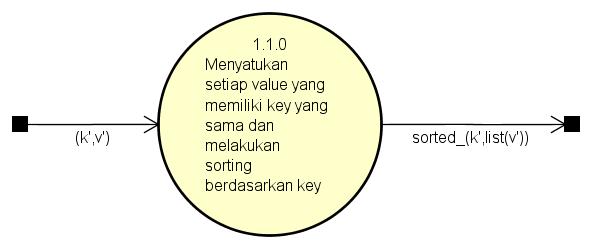
\includegraphics[scale=0.65]{Diagram/DFD_1_2_Training_Test_SS}
	\caption[DFD level 2: proses 1.1]{DFD level 2: proses 1.1}
	\label{fig:DFD level 2: proses 1.1}
\end{figure}

\paragraph{Data Dictionary pada DFD \textit{level} 2: proses 1.1}
\begin{enumerate}
	\item{Data \verb|(k',v')|} memiliki format yang sama dengan data \verb|output(k',v')| pada proses 1.0
	
	\item{Data \verb|sorted(k',list(v'))|} memiliki format yang sama dengan \textit{value} pada data \verb|output(k',v')|. Hanya saja value yang ini baru merupakan kumpulan dari \textit{value} yang memiliki \textit{key}(nama kelas) yang sama.

\end{enumerate}

\paragraph{DFD \textit{level} 2: pada proses 1.2}
\begin{figure}[H]
	\centering
	\includegraphics[scale=0.6]{Diagram/DFD_1_3_Testing_Red}
	\caption[DFD level 2: proses 1.2]{DFD level 2: proses 1.2}
	\label{fig:DFD level 2: proses 1.2}
\end{figure}

\paragraph{Data Dictionary pada DFD \textit{level} 2: proses 1.2}
\begin{enumerate}
	\item Data \verb|data_info| memiliki format dan isi yang sama dengan data \verb|data_info| pada proses 1.0
	
	\item Data \verb|processed_file_info|
	memiliki format dan isi yang mirip dengan data \verb|processed_file_info| pada proses 1.0. Hanya saja tidak mengikutsertakan nilai \textit{laplaciansmoothingadder}.

	\item Data \verb|sorted_(k',list(v'))|
	memiliki format dan isi yang sama dengan data \verb|sorted_(k',list(v'))| pada proses 1.1.

	\item Data \verb|(k",v")|
	\begin{enumerate}
		\item \textit{Key} terdiri dari:
		\begin{itemize}
			\item \textit{Class Name} = [A..Z|a..z]
			\item \textit{Confusion Matrix} = matrix $n*m$
		\end{itemize}

		\item \textit{Value} terdiri dari:
		\begin{itemize}
			\item \textit{Confusion Matrix} untuk tiap kelas = matrix $n*m$
			\item \textit{Error rate} untuk $Accuracy$ untuk tiap kelas = [0..9]
			\item \textit{Error rate} untuk $Recall$ untuk tiap \textit{class value} = [0..9]
			\item \textit{Error rate} untuk $Precision$ untuk tiap \textit{class value} = [0..9]
			\item \textit{Error rate} untuk $F-Measure$ untuk tiap \textit{class value} = [0..9]
		\end{itemize}
		Contoh data \verb|output(k",v")|
		\begin{lstlisting}
		<- Key ->
		@play
		####
		|		|	no	| yes	|
		| no	|	3	| 0		|
		| yes	|	0	| 2		|
		####
		<- Value ->
		Accuracy: 5/5 = 1.0
		*For Value = no
		Precision: -> 3 / 3 + 0 = 1.0
		Recall: -> 3 / 3 + 0 = 1.0 
		*For Value = yes
		Precision: -> 2 / 2 + 0 = 1.0
		Recall: -> 2 / 2 + 0 = 1.0
		F-Measure -> 0.8
		\end{lstlisting}
	\end{enumerate}

\end{enumerate}

\paragraph{P-Spec (\textit{Process Specification}) pada proses 1.0}

\begin{figure}[H]
	\centering
	\includegraphics[scale=0.65]{PSpec/P-Spec_dfd_1_2_0_test}
	\caption[P-Spec testing reduce: pada proses 1.2.0]{P-Spec testing reduce: pada proses 1.2.0}
	\label{fig:P-Spec testing reduce: pada proses 1.2.0}
\end{figure}

\begin{figure}[H]
	\centering
	\includegraphics[scale=0.65]{PSpec/P-Spec_dfd_1_2_1_test}
	\caption[P-Spec testing reduce: pada proses 1.2.1]{P-Spec testing reduce: pada proses 1.2.1}
	\label{fig:P-Spec testing reduce: pada proses 1.2.1}
\end{figure}


\subsubsection{Modul Klasifikasi \textit{Naive Bayes}}

Pada modul ini, program juga akan memanfaatkan model klasifikasi naive bayes yang telah dibuat sebelumnya untuk melakukan klasifikasi. Program pada modul ini dapat menerima 1 jenis input yang merupakan input manual secara satu - persatu atribut yang diperlukan untuk melakukan klasifikasi (\textit{predict new case}).

Berikut merupakan diagram \textit{flow chart} untuk modul klasifikasi:

\begin{figure}[H]
	\centering
	\includegraphics[scale=0.65]{Diagram/Flowchart_Klasifikasi}
	\caption[Flow Chart Modul Klasifikasi]{Flow Chart Modul Klasifikasi}
	\label{fig:Flow Chart Modul Klasifikasi}
\end{figure}

\subsection{Diagram Kelas}

Perangkat lunak yang dibangun akan mengikuti metode pemrograman berbasis objek (\textit{Object Oriented Programming}). Sehingga, untuk melakukan pemodelan pada perangkat lunak yang dibuat akan menggunakan kelas yang memiliki beberapa atribut dan metode operasi. Berikut merupakan gambaran diagram kelas pada perangkat lunak untuk setiap modul.

\subsubsection{Modul Kelola \textit{Input}}

\begin{figure}[H]
	\centering
	\includegraphics[scale=0.7]{ClassDiagram/Simple_CD_Input}
	\caption[Diagram kelas modul kelola input]{Diagram kelas modul kelola input}
	\label{fig:Diagram kelas modul kelola input}
\end{figure}

Pada modul ini, akan dibuatkan 2 kelas utama untuk menangani proses memasukkan file input ke dalam HDFS. Kelas tersebut diantaranya adalah:
\begin{enumerate}
\item{\textit{InputController.class}} \\
Kelas ini akan menjadi sebagai kelas yang meng-enkapsulasi seluruh proses penting yang dibutuhkan untuk memasukan file input ke dalam HDFS. Kelas ini hanya membuatkan satu method untuk melakukan operasi input yang akan diakses oleh user. Kelas ini akan memiliki objek instansiasi dari kelas \textit{HdfsService.class} dan memanggil beberapa method di dalamnya untuk melakukan operasi penulisan ke dalam HDFS.
\item{HdfsService.class} \\
Kelas ini akan mengatur segala kebutuhan yang diperlukan untuk melakukan proses penulisan ke dalam HDFS. Kelas ini akan memiliki koneksi terhadap HDFS Master sebagai \textit{hadoop client} untuk memerintahkan penulisan dan pendistribusian file baru yang akan dimasukkan ke dalam HDFS.
\end{enumerate}

\subsubsection{Modul \textit{Training dan Testing Naive Bayes M-R Based}}

\begin{figure}[H]
	\centering
	\includegraphics[scale=0.54]{ClassDiagram/Class_Diagram_Train_Test_MR}
	\caption[Diagram kelas modul \textit{training} dan \textit{testing}]{Diagram kelas modul \textit{training} dan \textit{testing}}
	\label{fig:Diagram kelas modul training dan testing}
\end{figure}

Pada modul ini, akan dibuatkan 3 kelas utama untuk menangani proses \textit{training} dan \textit{testing} berbasis \textit{MapReduce}. Di dalam kelas tersebut terdapat operasi - operasi untuk menjalankan proses \textit{MapReduce} pada modul training dan testing. Operasi - operasi ini telah dijelaskan sebelumnya pada Paragraf~\ref{par:contextdiagramTraining} dan Paragraf~\ref{par:contextdiagramTesting}. Berikut merupakan pemetaan fungsi pada kelas diagram yang akan dibuat dan proses \textit{MapReduce} pada DFD yang telah dibuat sebelumnya:

\begin{table}[H]
	\label{tab:mapDFDProcesstoClassDiagramFunction}
	\centering
	\caption{Pemetaan Proses \textit{MapReduce} Pada DFD Dengan Operasi Pada Diagram Kelas}
	\begin{tabular}{ | c | c | c | c | }
	\hline
	Nomor & Proses DFD & Operasi pada kelas & Section\\ \hline \hline
	1 & DFD level 1 modul \textit{training} Proses 1.0 Map & MyMapper.map() & figure~\ref{fig:DFD level 1 modul Training} \\ \hline
	2 & DFD level 1 modul \textit{training}: Proses 1.2 Reduce & MyReducer.reduce() & figure~\ref{fig:DFD level 1 modul Training} \\ \hline
	3 & DFD level 1 modul \textit{testing}: Proses 1.0 Map & MyMapper.map() & figure~\ref{fig:DFD level 1 modul Testing} \\ \hline
	4 & DFD level 1 modul \textit{testing}: Proses 1.2 Reduce & MyReducer.reduce() & figure~\ref{fig:DFD level 1 modul Testing} \\ \hline
	\end{tabular}
\end{table}

Berikut merupakan penjelasan 3 kelas 3 kelas utama untuk menangani proses \textit{training} dan \textit{testing} berbasis \textit{MapReduce}:

\begin{enumerate}
\item{App.class} \\
Kelas ini akan menjadi kelas utama yang akan menjalankan operasi \textit{testing} maupun \textit{training} yang berbasis \textit{MapReduce}. Pada kelas ini akan ditentukan pula kelas mana saja yang akan dijadikan sebagai kelas mapper dan kelas reducer nya, begitu juga dengan pasangan \textit{key} dan \textit{value} untuk \textit{input} dan untuk \textit{output} di setiap kelas.
\item{MyMapper.class} \\
Kelas ini akan menjalankan operasi pada fase map untuk proses training dan testing berbasis \textit{MapReduce}.
\item{MyReducer.class} \\
Kelas ini akan menjalankan operasi pada fase reduce untuk proses training dan testing berbasis \textit{MapReduce}.
\end{enumerate}

\subsubsection{Modul Klasifikasi \textit{Naive Bayes}}
\begin{figure}[H]
	\centering
	\includegraphics[scale=0.65]{ClassDiagram/Simple_CD_Klasifikasi}
	\caption[Diagram kelas modul klasifikasi \textit{naive bayes}]{Diagram kelas modul klasifikasi \textit{naive bayes}}
	\label{fig:Diagram kelas modul klasifikasi naive bayes}
\end{figure}

Pada modul ini, akan dibuatkan 10 kelas utama dan 2 kelas yang bertipe emum untuk menangani proses klasifikasi menggunakan model yang telah dibuat sebelumnya. Kelas tersebut diantaranya adalah: 
\begin{enumerate}
\item{\textit{TestingController.class}} \\
Kelas ini merupakan kelas utama yang akan melakukan enkapsulasi seluruh proses penting yang akan dijalankan pada proses klasifikasi.
\item{\textit{TestingUtils.class}} \\
Kelas ini akan menjadi kelas-pembantu pada kelas \textit{TestingController.class} untuk melakukan operasi - operasi yang dibutuhkan pada algoritma klasifikasi \textit{naive bayes}. Seperti perhitungan probabilitas posterior dan normal distribusi
\item{\textit{BayesianModel.class}} \\
Kelas ini merupakan kelas utama untuk merepresentasikan model klasifikasi \textit{naive bayes} yang telah dibuat sebelumnya.
\item{\textit{ModelType.enum}} \\
Enum ini akan menjadi tipe untuk setiap model yang ada pada kelas \textit{BayesianModel}. Enum tersebut terdiri antara: DISCRETE, NUMERIC, dan CLASS.
\item{\textit{ClassInfo.class}} \\
Kelas ini akan merepresentasikan seluruh atribut kelas pada model klasifikasi \textit{naive bayes} yang telah dibuat sebelumnya.
\item{\textit{ClassInfoDetail.class}} \\
Kelas ini merupakan ekstensi dari kelas \textit{ClassInfo.class}. Kelas ini akan menyimpan seluruh detail mengenai atribut kelas tertentu pada model \textit{naive bayes} yang sudah jadi.
\item{\textit{ErrorRate.class}} \\
Kelas ini akan merepresentasikan perhitungan \textit{ErrorRate} yang dapat dihitung setelah melakukan testing terhadap model \textit{naive bayes} yang sudah jadi sebelumnya.
\item{\textit{ErrorType.enum}} \\
Enum ini akan menjadi tipe untuk tiap error yang ada. Enum tersebut terdiri dari: $ACCURACY$, $PRECISION$, $RECALL$, dan $F_MEASURE$.
\item{\textit{ConfusionMatrix.class}} \\
Kelas ini akan merepresentasikan \textit{ConfusionMatrix} yang akan diperoleh setelah menjalani testing/klasifikasi pada model \textit{naive bayes} yang sudah jadi sebelumnya.
\item{\textit{ConfusionMatrixDetail.class}} \\
Kelas ini merupakan ekstensi dari kelas \textit{ConfusionMatrix.class}. Kelas ini akan menyimpan seluruh detail yang dimiliki oleh tiap instansiasi dari kelas \textit{ConfusionMatrix}.
\item{\textit{PredictorInfo.class}} \\
Kelas ini akan merepresentasikan sebagai seluruh atribut prediktor yang digunakan pada model \textit{naive bayes}.
\item{\textit{PredictorInfoDetail.class}} \\
Kelas ini merupakan kelas ekstensi dari kelas \textit{PredictorInfo.class}. Kelas ini akan menyimpan seluruh detail pad tiap instansiasi dari kelas \textit{PredictorInfo}.
\end{enumerate}
}{}
\ifdefstring{\vbabd}{1}{\chapter{Perancangan}
Berdasarkan analisis yang telah dilakukan, terdapat beberapa hal yang perlu dirancang untuk pembangunan perangkat lunak naive bayes berbasis \textit{hadoop mapreduce}. Pada bab ini dijelaskan perancangan yang diperlukan untuk membangun perangkat lunak yaitu perancang-
an antarmuka, diagram kelas rinci, serta rincian metode.
			
\section{Perancangan Antarmuka}
\label{sec:Perancangan Antarmuka}

Perangkat lunak \textit{naive bayes classification} memiliki 6 buah tampilan untuk yang tidak berbasis \textit{MapReduce}, yaitu: (1) \textit{Dashboard} (2) \textit{Input Set Manager} (3) \textit{Renew Model Manager} (4) \textit{Testing Manager} (5) \textit{Classification Manager} (6) \textit{Error Rate Dashboard}. Untuk program yang berbasis \textit{MapReduce} tidak memiliki antarmuka yang khusus, karena program hanya perlu dijalankan dengan menggunakan CLI (\textit{command line interface}). Berikut adalah penjelasan dan gambar dari tiap antarmuka yang dirancang:

\subsection{\textit{Dashboard}}
\label{subsec:Dashboard}

\begin{figure}[H]
	\centering
	\includegraphics[scale=0.45]{Mockup/mockup_dashboard_0}
	\caption[input-set-gui-1]{Dashboard}
	\label{fig:input-set-gui-1}
\end{figure}
\textit{Dashboard} dibuat untuk memudahkan user dalam memonitor model NBC yang telah dimasukkan ke dalam perangkat lunak yang dibangun. Berikut penjelasan lebih lanjut mengenai tiap komponen pada rancangan \textit{dashboard} yang dibuat:
\begin{enumerate}
	\item Berisi nama - nama atribut kelas dan total frekeunsi kemunculannya tiap nilai.
	\item Berisi nama - nama atribut prediktor dan frekuensi kemunculannya untuk prediktor bertipe diskrit dan \textit{mean} \verb|&| \textit{sigma} untuk yang bertipe numerik.
	\item \textit{Bayesian model} merupakan model dari NBC yang digunakan untuk testing dan klasifikasi. Model ini merupakan model yang langsung di-import dari hasil training di dalam HDFS.
\end{enumerate}

\subsection{\textit{Input Set Manager}}
\label{subsec:Input Set Manager}

\begin{figure}[H]
	\centering
	\includegraphics[scale=0.4]{Mockup/input-set-gui-1}
	\caption[\textit{Input Set Manager}]{\textit{Input Set Manager}}
	\label{fig:Input Set Manager}
\end{figure}
\textit{Input Set Manager} dibuat untuk memudahkan user melakukan input data ke dalam HDFS menggunakan perangkat lunak yang dibuat. Berikut penjelasan lebih lanjut mengenai tiap komponen pada rancangan \textit{Input Set Manager} yang dibuat:
\begin{enumerate}
	\item User dapat memilih tipe model input yang sudah ada dalam HDFS.
	\item Jika ingin membuat tipe model input baru pada HDFS, maka user perlu mengisi kolom ini dan mengisi nama model yang diinginkan.
	\item User dapat memilih file input yang dikirimkan ke dalam HDFS. User dapat memilih > 1 file sekaligus.
	\item User dapat memilih file info mengenai file input, yang dikirimkan ke dalam HDFS.
	\item User dapat memilih presentase pembagian data antara data \textit{training} dan data \textit{testing} dari keseluruhan data input yang dimasukkan ke dalam HDFS.
	\item Setelah memillih file info, user dapat memilih atribut mana saja yang digunakan untuk training. User juga dapat memilih tipe(diskrit/numerik) dari atribut tersebut beserta jenisnya (kelas/prediktor).
\end{enumerate}

\subsection{\textit{Renew NBC Model Manager}}
\label{subsec:Renew Model Manager}

\begin{figure}[H]
	\centering
	\includegraphics[scale=0.45]{Mockup/mockup_renewmodel_manager}
	\caption[\textit{Renew NBC Model Manager}]{\textit{Renew NBC Model Manager}}
	\label{fig:Renew Model Manager}
\end{figure}
\textit{Renew Model Manager} dibuat agar user selalu bisa memperbaharui model NBC pada perangkat lunak yang dibuat.
\begin{enumerate}
	\item User dapat memilih file model NBC hasil dari training dari sistem penyimpanan \textit{local}.
	\item User dapat memilih file model NBC hasil dari training langsung dari HDFS.
\end{enumerate}

\subsection{\textit{Testing Manager}}
\label{subsec:Testing Manager}

\textit{Testing Manager} dibuat untuk melakukan testing pada model NBC yang sudah di-import ke dalam program sebelumnya.

\begin{figure}[H]
	\centering
	\includegraphics[scale=0.45]{Mockup/mockup_testing_manager}
	\caption[\textit{Testing Manager}]{\textit{Testing Manager}}
	\label{fig:Testing Manager}
\end{figure}
\begin{enumerate}
	\item User dapat memilih file input dan file info dari penyimpanan \textit{local} milik user.
	\item User dapat memilih file testing yang sudah ada di dalam HDFS dengan memilih model input direktori pada HDFS.
\end{enumerate}

\subsection{\textit{Classification Manager}}
\label{subsec:Classification Manager}

\begin{figure}[H]
	\centering
	\includegraphics[scale=0.45]{Mockup/mockup_classification_manager}
	\caption[\textit{Classification Manager}]{\textit{Classification Manager}}
	\label{fig:Classification Manager}
\end{figure}
\textit{Classification Manager} dapat digunakan untuk mengklasifikasi satu record input/kasus yang secara langsung diisi sendiri oleh user yang menggunakannya terhadap model NBC yang sudah ada pada perangkat lunak sebelumnya.
\begin{enumerate}
	\item User memilih nilai prediktor untuk kasus baru (prediktor dapat berupa dropdown untuk yang bertipe diskrit dan \textit{number} untuk yang bertipe numerik)
	\item User dapat memilih kelas yang menjadi prediksi sebelumnya dari user untuk diperiksa kebenarannya jika menggunakan program setelah diklasifikasikan menggunakan model NBC yang sudah ada.
	\item Hasil dari klasifikasi yang telah dijalankan.
\end{enumerate}

\subsection{\textit{Error Rate Dashboard}}
\label{subsec:Error Rate Dashboard}

\begin{figure}[H]
	\centering
	\includegraphics[scale=0.45]{Mockup/mockup_errorrate}
	\caption[\textit{Error Rate Dashboard}]{\textit{Error Rate Dashboard}}
	\label{fig:Error Rate Dashboard}
\end{figure}
\textit{Error Rate Dashboard} dibuat untuk memonitor hasil \textit{error rate} yang sudah dihitung setelah menjalani proses testing. 
\begin{enumerate}
	\item \textit{Confusion matrix} untuk setiap atribut kelas.
	\item Error rate yang dihasilkan setelah melakukan klasifikasi meliputi: (1)$Accuracy$; (2)$Precision$; (3)$Recall$; (4)$F-Measure$.
\end{enumerate}



\section{Diagram Kelas Lengkap}
Berikut adalah penjelasan dari kelas - kelas pada keempat modul yang dibuat beserta penjelasan setiap atribut dan operasi yang dimiliki oleh kelas - kelas tersebut.

\subsection{Diagram Kelas Modul \textit{Train Naive Bayes M-R Based}}
Pada diagram kelas ini terdapat terdapat 2 \textit{package} utama yang menjadi inti dari modul ini, salah satunya merupakan \textit{package} yang dimiliki oleh \textit{library} dari \textit{hadoop client} untuk dapat menjalankan proses \textit{mapreduce}. Pada diagram kelas modul ini, terdapat sedikit perbedaan dengan yang sudah dianalisis pada Bab~\ref{subsubsec:Modul Training dan Testing Naive Bayes M-R Based}. Terdapat penambahan kelas yang bernama \texttt{MyCombiner} di dalam package \texttt{combiner}. Berikut adalah penjelasan dan gambar dari \textit{package - package} dan kelas - kelas tersebut:
\begin{figure}[H]
	\centering
	\includegraphics[scale=0.6]{ClassDiagramLengkap/CD_Train_MR}
	\caption[Diagram Kelas \textit{Train Naive Bayes M-R Based}]{\textit{Diagram Kelas Train Naive Bayes M-R Based}}
	\label{fig:Diagram Kelas Modul Kelola Input}
\end{figure}

\paragraph{\textit{Package} $org.apache.hadoop.mapreduce$}
Dalam \textit{package} ini terdapat 2 kelas utama yang menjadi kelas \textit{parent} dari kelas \textit{reducer} dan \textit{mapper} yang di-implementasikan.
\begin{enumerate}
	\item{Kelas \textit{Mapper}}\\
	Kelas ini memiliki 4 buah \textit{generic types}\footnote{A generic type is a generic class or interface that is parameterized over types \cite{GenericTypeJavaOracle}} yang perlu di-implementasikan pada kelas yang mengimplementasi method ini. Parameter \textit{generic types} tersebut antara lain adalah:
	\begin{itemize}
		\item{\textit{KEYIN}}\\
		Kelas ini merupakan tipe kelas yang menjadi \textit{key} masukan pada proses Map untuk program \textit{Mapreduce} yang dibuat.		
		\item{\textit{VALUEIN}}\\
		Merupakan tipe kelas yang menjadi \textit{value} dari masukan pada proses Map untuk program \textit{Mapreduce} yang dibuat.
		\item{\textit{KEYOUT}}\\
		Merupakan tipe kelas yang menjadi \textit{key} keluaran pada proses Map untuk program \textit{Mapreduce} yang dibuat.
		\item{\textit{VALUEOUT}}\\
		Merupakan tipe kelas yang menjadi \textit{value} keluaran pada proses Map untuk program \textit{Mapreduce} yang dibuat.
	\end{itemize}
	
	\item{Kelas \textit{Reducer}}\\
	Kelas ini memiliki 4 buah \textit{generic types} yang perlu di-implementasikan pada kelas yang mengimplementasi method ini. Parameter \textit{generic types} tersebut antara lain adalah:
	\begin{itemize}
		\item{\textit{KEYIN}}\\
		Kelas ini merupakan tipe kelas yang menjadi \textit{key} masukan pada proses \textit{Reduce} untuk program \textit{Mapreduce} yang dibuat.		
		\item{\textit{VALUEIN}}\\
		Merupakan tipe kelas yang menjadi \textit{value} dari masukan pada proses \textit{Reduce} untuk program \textit{Mapreduce} yang dibuat.
		\item{\textit{KEYOUT}}\\
		Merupakan tipe kelas yang menjadi \textit{key} keluaran pada proses \textit{Reduce} untuk program \textit{Mapreduce} yang dibuat.
		\item{\textit{VALUEOUT}}\\
		Merupakan tipe kelas yang menjadi \textit{value} keluaran pada proses \textit{Reduce} untuk program \textit{Mapreduce} yang dibuat.
	\end{itemize}
\end{enumerate}

\paragraph{\textit{Package} $mczal.bayes$}
Dalam \textit{package} ini terdapat beberapa \textit{package} lagi dan kelas - kelas yang dijadikan implementasi dari kelas \textit{Mapper} dan \textit{Reducer} pada package \textit{org.apache.hadoop.mapreduce} untuk proses \textit{MapReduce}.
\begin{enumerate}
	\item{Kelas \texttt{TrainApp}}\\
	Kelas ini merupakan kelas utama(\textit{main class}) yang dijalankan pertama kali program ini dieksekusi. Kelas ini memiliki 1 atribut \textit{static} dan 1 method \textit{main}.
	\begin{enumerate}
		\item Atribut \verb|HDFS_AUTHORITY| \\
		Atribut ini bertipe \textit{String} dan memiliki \textit{modifier} \textit{static} dan \textit{final} agar nilainya tidak dapat diubah - ubah. Inisialisasi pertama dari atribut ini adalah: \verb|"hdfs://master:9000"|. \verb|"hdfs://master:9000"| merupakan url dari node master yang digunakan untuk dapat berkomunikasi dengan node master pada lingkungan \textit{hadoop}. Atribut ini digunakan untuk \textit{request} operasi baca file \textit{meta.info} pada HDFS.
		
		\item Operasi \verb|main|\\
		Operasi ini menjadi operasi pertama yang dijalankan ketika melakukan eksekusi program mapreduce pada modul ini. Operasi ini men-\textit{set} kelas \textit{mapper} dan kelas \textit{reducer} yang digunakan serta variabel - variabel yang perlu dikirimkan kepada tiap node yang dibutuhkan oleh mereka.
	\end{enumerate}

	\item{Kelas \texttt{MyTrainingMapper}}\\
	Kelas ini merupakan kelas turunan dari kelas \textit{Mapper} yang ada pada package \verb|org.apache.hadoop.mapreduce|. \textit{Generic type} kelas parent dari kelas ini adalah:
	\begin{enumerate}
		\item{Object} merupakan tipe \textit{key} masukan dari proses \textit{map}.
		\item{Text} merupakan tipe \textit{key} masukan dari proses \textit{map}. Karena, data masukan berupa \textit{string}.
		\item{Text} merupakan tipe \textit{key} keluaran dari proses \textit{map}. Karena, \textit{key} pada hasil dari fase \textit{map} mengeluarkan data yang bertipe \textit{string}.
		\item{DoubleWritable} merupakan tipe \textit{value} keluaran dari proses \textit{map}. Karena, \textit{value} keluaran pada proses \textit{map} berisi jumlah frekuensi atau nilai dari atribut prediktor-numerik yang bertipe numerik.
	\end{enumerate}
	Kelas ini memiliki 8 atribut. Diantaranya adalah:
	\begin{enumerate}
		\item \verb|_CLASS| merupakan atribut bertipe \textit{string} yang memiliki \textit{modifier} \textit{static} dan \textit{final}. Atribut ini memiliki nilai inisialisasi awal = $"|$\verb|_|$class|"$ yang digunakan untuk membedakan bahwa data keluaran yang memiliki string berisi $"|$\verb|_|$class|"$ merupakan data keluaran yang digunakan untuk menghitung jumlah frekuensi dari kemunculan atribut bertipe kelas.
		\item \verb|_DISCRETE| merupakan atribut bertipe \textit{string} yang memiliki \textit{modifier} \textit{static} dan \textit{final}. Atribut ini memiliki nilai inisialisasi awal = $"|disc|"$ yang digunakan untuk membedakan bahwa data keluaran yang memiliki string berisi $"|disc|"$ merupakan data keluaran yang digunakan untuk menghitung jumlah frekuensi dari kemunculan atribut prediktor bertipe diskrit berdasarkan atribut kelas tertentu.
		\item \verb|_CONTINUOUS| merupakan atribut bertipe \textit{string} yang memiliki \textit{modifier} \textit{static} dan \textit{final}. Atribut ini memiliki nilai inisialisasi awal = $"|cont|"$ yang digunakan untuk membedakan bahwa data keluaran yang memiliki string berisi $"|cont|"$ merupakan data keluaran yang digunakan untuk mencatat nilai dari atribut numerik berdasarkan atribut kelas tertentu.
		\item \verb|DISCRETE_TYPE| merupakan atribut bertipe \textit{string} yang memiliki \textit{modifier} \textit{static} dan \textit{final}. Atribut ini memiliki nilai inisialisasi awal = $"DISCRETE"$ yang digunakan untuk membedakan bahwa data input setelah displit dengan regex ',' pada indeks tertentu memiliki info bertipe diskrit.
		\item \verb|NUMERIC_TYPE| merupakan atribut bertipe \textit{string} yang memiliki \textit{modifier} \textit{static} dan \textit{final}. Atribut ini memiliki nilai inisialisasi awal = $"NUMERICAL"$ yang digunakan untuk membedakan bahwa data input setelah displit dengan regex ',' pada indeks tertentu memiliki info bertipe numerik.
		\item \verb|one| merupakan atribut bertipe \textit{DoubleWritable} yang memiliki \textit{modifier} \textit{static}. Atribut ini memiliki nilai inisialisasi awal = integer bernilai 1 yang digunakan untuk mencatat tiap kemunculan atribut prediktor terhadap atribut kelas tertentu yang sedang diperiksa dengan jumlah kemunculan sebanyak 1.
		\item \verb|wordAttr| merupakan atribut bertipe \textit{Text} yang memiliki \textit{modifier} \textit{static}. Atribut ini digunakan untuk mencatat tiap atribut prediktor yang ditulis menjadi \textit{output key} untuk perhitungan probabilitas posterior dari atribut tertentu pada atribut kelas tertentu.
		\item \verb|wordClass| merupakan atribut bertipe \textit{Text} yang memiliki \textit{modifier} \textit{static}. Atribut ini digunakan untuk mencatat tiap kemunculan atribut kelas tertentu dan ditulis menjadi \textit{output key} untuk perhitungan frekuensi atribut kelas.
	\end{enumerate}
	Kelas ini memiliki 1 buah operasi. Operasi tersebut adalah operasi \textit{map(key : Object, value : Text, context : Context) : void} yang melakukan operasi pada fase map untuk proses training pada modul ini. Seperti yang digambarkan pada DFD sebelumnya, proses ini melakukan perhitungan jumlah frekuensi kemunculan tiap atribut. Terkecuali untuk atribut prediktor yang bertipe numerik, operasi ini mengeluarkan kembali nilai yang dibaca dari input.
	
\begin{algorithm}[H]
\caption{NBC Model Map Algorithm}\label{alg:NBCGenMap}
\begin{algorithmic}[1]
\Procedure{Map}{$key,value,context$}\Comment{Map function}
\State \verb|_|\texttt{CLASS} $\gets$ \texttt{"|}$\verb|_|$\texttt{class|"}
\State \verb|_|\texttt{DISCRETE} $\gets$ \texttt{"|disc|"}
\State \verb|_|\texttt{CONTINUOUS} $\gets$ \texttt{"|cont|"}
\State \texttt{one} $\gets$ \texttt{1}
\State \texttt{NUMERIC}\verb|_|\texttt{TYPE} $\gets$ \texttt{"NUMERICAL"}
\State \texttt{DISCRETE}\verb|_|\texttt{TYPE} $\gets$ \texttt{"DISCRETE"}

\State \texttt{countColumn} $\gets$ \texttt{getInputColumnCount}
\State \texttt{inputSplit[]} $\gets$ \texttt{value.split(',')}
\If{\texttt{inputSplit.length != countCols}}\Comment{Ignoring missing values}
	\State \Return
\EndIf

\State \texttt{classConf} $\gets$ getClassInfo \Comment{\texttt{get class info from meta.info}}
\State \texttt{classSplitConf[]} $\gets$ \texttt{classConf.split(";")}

\State \texttt{attrConf} $\gets$ \texttt{getAttributeInfo} \Comment{\texttt{get predictor info from meta.info}}
\State \texttt{attrSplitConf[]} $\gets$ \texttt{attrConf.split(";")}

\State \texttt{checkerClassPrior} $\gets$ \texttt{classSplitConf.length}
%\For $i \gets 0$ \To $attrSplitConf.length$ \Do
\For{$i \gets 0$ \textbf{to} \texttt{attrSplitConf.length}}	
	\If{\texttt{attrSplitConf[i].split(",")[2].equals(DISCRETETYPE)}}
		%\For $j \gets 0$ \To $classSplitConf.length$ \Do
		\For{$j \gets 0$ \textbf{to} \texttt{classSplitConf.length}}	
			\State currKey $ \gets $ \verb|_|\texttt{DISCRETE + attrSplitConf[i].split(",")[0]}
              \texttt{+ "," + inputSplit[Integer.parseInt(attrSplitConf[i]}
              \texttt{.split(",")[1])]}
              \texttt{+ "," + classSplitConf[j].split(",")[0]}
              \texttt{+ "," + inputSplit[Integer.parseInt(classSplitConf[j]}
              \texttt{.split(",")[1])];}
          	\State \texttt{wordAttr.set(currKey);}
          	\State \texttt{context.write(wordAttr, one)}
		\EndFor
	\EndIf
\EndFor

\EndProcedure
\end{algorithmic}
\end{algorithm}
	
	\item{Kelas \texttt{MyTrainingReducer}}\\
	Kelas ini merupakan kelas turunan dari kelas \textit{Reducer} pada \textit{package org.apache.hadoop.mapreduce}. \textit{Generic type} kelas parent dari kelas ini adalah: 
	\begin{enumerate}
		\item Text merupakan tipe \textit{key} masukan dari proses \textit{reduce} yang dikirim dari proses sebelumnya yaitu proses \textit{map}
		\item DoubleWritable merupakan tipe \textit{value} masukan dari proses \textit{reduce} yang dikriim dari proses sebelumnya yaitu proses \textit{map}.
		\item Text merupakan tipe \textit{key} keluaran dari proses \textit{reduce}. Karena data keluaran berupa model NBC memiliki key berisi string.
		\item Text merupakan tipe \textit{value} keluaran dari proses \textit{reduce}. Karena data keluaran berupa model NBC memiliki \textit{value} berisi string.
	\end{enumerate}
	Kelas ini memiliki 3 atribut yang memiliki \textit{modifier} \textit{static} dan \textit{final}. Atribut tersebut diantaranya adalah:
	\begin{enumerate}
		\item \verb|CLASS_TYPE| merupakan atribut bertipe string yang memiliki nilai inisialisasi awal = \textit{"CLASS"}. Atribut ini digunakan sebagai pembeda pada data keluaran yang merupakan atribut kelas.
				
		\item \verb|DISCRETE_TYPE| merupakan atribut bertipe string yang memiliki nilai inisialisasi awal = \textit{"DISCRETE"}. Atribut ini digunakan sebagai pembeda pada data keluaran yang merupakan atribut prediktor bertipe diskrit.

		\item \verb|NUMERIC_TYPE| merupakan atribut bertipe string yang memiliki nilai inisialisasi awal = \textit{"NUMERIC"}. Atribut ini digunakan sebagai pembeda pada data keluaran yang merupakan atribut prediktor bertipe numerik.
	\end{enumerate}
	
	Kelas ini memiliki 1 buah operasi. Operasi tersebut adalah operasi \textit{reduce(key : Text, values : Iterable<DoubleWritable>, context : Context) : void} yang melakukan operasi pada fase reduce untuk proses training pada modul ini. Seperti yang digambarkan pada DFD sebelumnya, proses ini melakukan akumulasi dari tiap perhitungan jumlah frekuensi kemunculan tiap value yang memiliki key yang sama. Terkecuali untuk atribut prediktor yang bertipe numerik, operasi ini menghitung nilai rata - rata dari tiap value pada key tersebut dan lalu dilanjutkan menghitung nilai standar deviasi pada probabilitas posterior atribut numerik tersebut.
	
	
\begin{algorithm}[H]
\caption{NBC Model Reduce Algorithm}\label{alg:NBCGenReduce}
\begin{algorithmic}[1]
\Procedure{Reduce}{$key,values[],context$}\Comment{Reduce function}

\State \verb|CLASS_TYPE| $\gets$ \texttt{"CLASS"}
\State \verb|DISCRETE_TYPE| $\gets$ \texttt{"DISCRETE"}
\State \verb|NUMERIC_TYPE| $\gets$ \texttt{"NUMERIC"}

\State \texttt{sum} $\gets 0$
\State \texttt{count} $\gets 0$
\State \texttt{caches} $\gets$ \texttt{List<Double>}

\ForAll{\texttt{value} $\in$ \texttt{values}}
	\State \texttt{caches.add(value)}
	\State \texttt{sum} $\gets$ \texttt{sum}$+$\texttt{value}
	\State \texttt{count}$++$
\EndFor

\If{\texttt{key.type} == \texttt{DISCRETE\_TYPE}}

\State \texttt{splitter} $\gets$ \texttt{key.split("|")[2]}
\State \texttt{result} $\gets$ \texttt{splitter + "," + sum + "|" +}\verb|DISCRETE_TYPE|
\State \texttt{write(result,"")}

\ElsIf{\texttt{key.type} $==$ \texttt{CLASS\_TYPE}}

\State \texttt{splitter} $\gets$ \texttt{key.split("|")[2]}
\State \texttt{result} $\gets$ \texttt{splitter + "," + sum + "|" +}\verb|CLASS_TYPE|
\State \texttt{write(result,"")}

\ElsIf{\texttt{key.type} $==$ \texttt{NUMERIC\_TYPE}}

\State \texttt{mean} $\gets$ \texttt{sum/count}
\State \texttt{calcTemp} $\gets$ \texttt{0.0}

\ForAll{\texttt{c} $\in$ \texttt{caches}}
	\State \texttt{calcTemp} $\gets$\texttt{calcTemp}$+(c - mean)^2$
\EndFor

\State \texttt{calcTemp} $\gets$ \texttt{calcTemp * (1/count)}
\State \texttt{sigma} $\gets calcTemp^{0.5}$
\State \texttt{result} $\gets$  \texttt{key.split("|")[2]}
\State \texttt{write(result, ";" + mean + "|" + sigma + "|" +}\verb|NUMERIC_TYPE|\texttt{)}

\EndIf

\EndProcedure
\end{algorithmic}
\end{algorithm}

\item Kelas \texttt{MyTrainingCombiner}
Kelas ini merupakan kelas yang akan menjadi \textit{combiner} pada modul ini. Kelas ini akan melakukan penyatuan data yang memiliki key sama pada node pekerja fase \textit{map} terlebih dahulu sebelum dikirimkan ke fase \textit{reducer}. Sama seperti pada kelas \texttt{MyTrainingReducer}, kelas ini juga merupakan turunan dari kelas \textit{Reducer} milik hadoop yang melakukan \textit{reducer} setelah proses \textit{map} tetapi masih berada pada \textit{node} pekerja fase \textit{map}. Kelas ini hanya memiliki 1 buah operasi yaitu operasi reduce yang berfungsi untuk menyatukan nilai yang memiliki key yang sama untuk dijumlahkan. Fase ini hanya akan menyatukan nilai dari atribut bertipe diskrit saja. Karena untuk atribut bertipe numerik, proses penyatuan perlu dilakukan pada fase reduce untuk kebutuhan melakukan perhitungan rata - rata dan standard deviasi. Berikut merupakan \textit{pseudocode} dari method \texttt{reduce(key : Text, values : Iterable<DoubleWritable>, context : Context) : void} milik kelas ini:

\begin{algorithm}[H]
\caption{NBC Model Combine Algorithm}\label{alg:NBCGenCombine}
\begin{algorithmic}[1]
\Procedure{Reduce}{$key,values[],context$}\Comment{Reduce function}

\State \verb|CLASS_TYPE| $\gets$ \texttt{"CLASS"}
\State \verb|DISCRETE_TYPE| $\gets$ \texttt{"DISCRETE"}
\State \verb|NUMERIC_TYPE| $\gets$ \texttt{"NUMERIC"}

\If{\texttt{key.type == \texttt{DISCRETE\_TYPE}} or \texttt{key.type == CLASS\_TYPE}}
	\State \texttt{sum = 0}
	\ForAll{\texttt{v} $\in$ \texttt{values}}
		\State \texttt{sum += v}
	\EndFor
	\State \texttt{context.write(key,sum)}
	
\ElsIf{\texttt{key.type == \texttt{NUMERIC\_TYPE}}}
	\ForAll{\texttt{v} $\in$ \texttt{values}}
		\State \texttt{context.write(key,sum)}
	\EndFor
\EndIf

\EndProcedure
\end{algorithmic}
\end{algorithm}


\end{enumerate}

\subsection{Diagram Kelas Modul \textit{Testing Naive Bayes M-R Based}}
Pada diagram kelas ini terdapat 1 kelas utama(\textit{main}) yang dijalankan pertama kali saat program dieksekusi dan 3 package utama yang merupakan implementasi dari modul \textit{testing naive bayes}. Untuk kelas yang berfungsi sebagai \textit{mapper} dan \textit{reducer} pada modul ini, sama dengan diagram kelas pada modul "\textit{Training Naive Bayes M-R Based}" merupakan kelas implementasi(kelas turunan) dari 2 kelas Mapper dan Reducer milik hadoop pada package \verb|org.apache.hadoop.mapreduce|. Karena bentuk relasi-nya sama persis dengan yang ada pada modul "\textit{Training Naive Bayes M-R Based}", pada modul ini tidak digambarkan relasi kelas mapper dan reducer dengan 2 kelas parent milik \textit{library hadoop}.

\subsubsection{Kelas \textit{Main}}
\begin{figure}[H]
	\centering
	\includegraphics[scale=0.7]{ClassDiagramLengkap/CD_Test_Main}
	\caption[Diagram Kelas Modul \textit{Testing: Main}]{Diagram Kelas Modul \textit{Testing: Main}}
	\label{fig:Diagram Kelas Modul Testing: Main}
\end{figure}
	Kelas \textit{TestingApp} ini merupakan kelas utama(\textit{main class}) yang dijalankan pertama kali program \textit{MapReduce} ini dieksekusi. Kelas ini memiliki 1 atribut \textit{static} dan 1 method \textit{main}.
	\begin{enumerate}
		\item Atribut \verb|HDFS_AUTHORITY| \\
		Atribut ini bertipe \textit{String} dan memiliki \textit{modifier} \textit{static} dan \textit{final} agar nilainya tidak dapat diubah - ubah. Inisialisasi pertama dari atribut ini adalah: \verb|"hdfs://master:9000"|. \verb|"hdfs://master:9000"| merupakan url dari node master yang digunakan untuk dapat berkomunikasi dengan node master pada lingkungan \textit{hadoop}. Atribut ini digunakan untuk \textit{request} operasi baca file \textit{meta.info} pada HDFS.
		
		\item Operasi \verb|main|\\
		Operasi ini menjadi operasi pertama yang dijalankan ketika melakukan eksekusi program mapreduce pada modul ini. Operasi ini men-\textit{set} kelas \textit{mapper} dan kelas \textit{reducer} yang digunakan serta variabel - variabel yang perlu dikirimkan kepada tiap node yang dibutuhkan oleh mereka.
	\end{enumerate}


\subsubsection{\textit{Package Base}}
\begin{figure}[H]
	\centering
	\includegraphics[scale=0.64]{ClassDiagramLengkap/CD_Test_BASE}
	\caption[Diagram Kelas Modul \textit{Testing: Package Base}]{Diagram Kelas Modul \textit{Testing: Package Base}}
	\label{fig:Diagram Kelas Modul Testing: Package Base}
\end{figure}

Pada package ini terdapat 3 kelas utama yang menjadi kelas \textit{parent}(\textit{superclass}) dari kelas - kelas yang mengimplementasikan-nya. Kelas - kelas parent pada package ini dibuat untuk memenuhi konsep inheritance yang baik dan menghindari terjadinya duplikasi kode pada kelas - kelas terseubt. Kelas - kelas ini juga meminimumkan kode yang nantinya dibuat. Berikut adalah penjelasan lebih lanjut mengenai tiap kelas serta atribut dan operasi yang dimilikinya:

\begin{enumerate}
	\item \texttt{Enum}\footnote{Enum adalah sebuah tipe data yang nilainya hanya terbatas dari pilihan nilai-nilai yang telah didefinisikan terlebih dahulu. \textit{Enumeration} di Java baru diperkenalkan pada versi Java 5.} \textit{Type}\\ ini berisi:
	\begin{enumerate}
		\item NUMERIC
		\item DISCRETE
		\item CLASS
	\end{enumerate}
	\textit{Enum} ini digunakan sebagai pengenal tipe dari tiap atribut yang ada pada model NBC.
	
	\item{Kelas \texttt{AttributeMetaInfo}}\\
	Kelas ini memiliki 1 buah parameter \textit{generic type} yang perlu diimplementasikan pada kelas yang menjadi turunan dari kelas ini. \textit{Generic type} pada kelas ini harus merupakan turunan dari kelas \texttt{AttributeDetail}. Kelas ini mencatat seluruh atribut(jenis: prediktor,kelas;tipe: numerik,diskrit) yang ada pada model NBC. Atribut yang dimiliki oleh kelas ini merupakan atribut yang merepresentasikan atribut pada model NBC secara umum. Atribut - atribut pada kelas ini adalah:
	\begin{enumerate}
		\item{\texttt{name}}\\ 
		Atribut ini bertipe \texttt{string} yang merepresentasikan nama dari atribut pada model NBC.

		\item{\texttt{type}}\\
		Atribut ini bertipe \texttt{Enum Type} yang merepresentasikan jenis dari atribut pada model NBC.

		\item{\texttt{sigma}}\\
		Atribut ini bertipe \texttt{double} yang merepresentasikan nilai standar deviasi dari keseluruhan data atribut ini pada model NBC jika dan hanya jika tipe dari atribut ini merupakan numerik. Jika tidak, maka nilai atribut ini selalu dikosongkan.

		\item{\texttt{mean}}\\
		Atribut ini bertipe \texttt{double} yang merepresentasikan nilai rata - rata dari keseluruhan data atribut ini pada model NBC jika dan hanya jika tipe dari atribut ini merupakan numerik. Jika tidak, maka nilai atribut ini selalu dikosongkan.

		\item{\texttt{attrDetailMap}}\\
		Atribut ini bertipe \texttt{Map} dengan \texttt{key=string} dan \texttt{value=T(generic type)} yang merepresentasikan kumpulan dari semua nilai yang dimiliki oleh atribut ini jika dan hanya jika tipe dari atribut ini merupakan diskrit atau atribut kelas. Jika tidak, maka nilai atribut ini selalu dikosongkan.
	\end{enumerate}
	
	Kelas ini menerima 2 buah operasi konstruktor untuk membuat instansiasi dan menginisialisasi nilai - nilai dari atribut di dalamnya. Konstruktor tersebut antara lain adalah:
	\begin{enumerate}
		\item \texttt{AttributeMetaInfo(name : String, type : Type)}\\
		Konstruktor ini digunakan untuk menginisialisasi atribut tanpa mengisi nilai dari atribut \texttt{sigma} dan \texttt{mean}. Konstruktor ini biasa digunakan untuk atribut bertipe \textit{non-numerik}.
		\item \texttt{AttributeMetaInfo(name : String, type : Type, sigma : double, mean : double)}\\
		Konstruktor ini digunakan untuk menginisialisasi atribut dengan mengisi seluruh atribut yang ada, kecuali \texttt{attrDetailMap}. Konstruktor ini biasa digunakan untuk atribut bertipe numerik.
		
	\end{enumerate}
	
	\item{Kelas \texttt{AttributeDetail}}\\
	Kelas ini merepresentasikan tiap nilai diskrit dari atribut diskrit/kelas yang ada pada model NBC. Selain mencatat nama dari nilai diskrit atribut diskrit/kelas pada NBC, kelas ini juga mencatat jumlah frekuensi dari atribut ini pada model NBC.
	Kelas ini memiliki 2 atribut dan 1 operasi konstruktor, diantaranya adalah:
	\begin{enumerate}
		\item Atribut \texttt{count} bertipe \texttt{integer} yang digunakan untuk mencatat jumlah frekuensi dari kemunculan nilai atribut ini.
		\item Atribut \texttt{value} bertipe \texttt{string} yang digunakan untuk mencatat nama dari nilai diskrit instansiasi dari kelas ini.
		\item Operasi konstruktor \texttt{AttributeDetail(value : String, count : int): void} menginisialisasi nilai awal seluruh atribut yang dimiliki oleh kelas ini pada saat instansiasi objek dari kelas ini.
	\end{enumerate} 
	
\end{enumerate}

\subsubsection{\textit{Package Mapper}}
\begin{figure}[H]
	\centering
	\includegraphics[scale=0.6]{ClassDiagramLengkap/CD_Test_Mapper}
	\caption[Diagram Kelas Modul \textit{Testing: Package Mapper}]{Diagram Kelas Modul \textit{Testing: Package Mapper}}
	\label{fig:Diagram Kelas Modul Testing: Package Mapper}
\end{figure}
Pada package ini terdapat 7 kelas utama yang digunakan untuk melakukan proses pada fase \textit{map} pada modul testing. Berikut merupakan penjelasan tiap package dan kelas - kelas yang ada pada \texttt{Package mapper}:
\begin{enumerate}
	\item{Kelas \texttt{MyTestingMapper}}\\
	Kelas ini merupakan kelas utama yang dijalankan pada proses map. Kelas ini memiliki 5 atribut dan 3 operasi yang digunakan untuk dapat melakukan operasi pada fase map secara keseluruhan. Berikut merupakan penjelasan mengenai atribut dan operasi pada kelas ini:
	\begin{itemize}
		\item{Atribut}
		\begin{enumerate}
			\item{\verb|HDFS_AUTHORITY|}\\
		Atribut ini bertipe \textit{String} dan memiliki \textit{modifier} \textit{static} dan \textit{final} agar nilainya tidak dapat diubah - ubah. Inisialisasi pertama dari atribut ini adalah: \verb|"hdfs://master:9000"|. \verb|"hdfs://master:9000"| merupakan url dari node master yang digunakan untuk dapat berkomunikasi dengan node master pada lingkungan \textit{hadoop}. Atribut ini digunakan untuk \textit{request} operasi baca file \textit{meta.info} dan model NBC pada HDFS.
		
		\item{\texttt{classContainer}}\\
		Atribut ini bertipe \texttt{ClassContainer} yang menyimpan seluruh model atribut NBC yang merupakan atribut kelas. 

		\item{\texttt{predictorContainer}}\\
		Atribut ini bertipe \texttt{PredictorContainer} yang menyimpan seluruh model atribut NBC yang merupakan atribut prediktor. 

		\item{\texttt{classSplitConf}}\\
		Atribut ini bertipe \texttt{array of string} yang menyimpan seluruh keterangan mengenai field - field yang merupakan atribut bertipe kelas yang digunakan pada model NBC. Keterangan yang disimpan pada atribut ini adalah: (1) nomor indeks; (2) name field; (3) jenis atribut. 

		\item{\texttt{attrSplitConf}}\\
		Atribut ini bertipe \texttt{array of string} yang menyimpan seluruh keterangan mengenai field - field yang merupakan atribut bertipe prediktor yang digunakan pada model NBC. Keterangan yang disimpan pada atribut ini adalah: (1) nomor indeks; (2) name field; (3) jenis atribut.
		
		\end{enumerate}
		
		\item{Operasi}
		\begin{enumerate}
			\item{\texttt{map(}}
			Operasi ini melakukan proses pada fase \textit{map} untuk proses testing pada modul ini. Proses yang dilakukan meliputi perhitungan nilai probabilitas posterior untuk setiap input pada value. Proses perhitungan tersebut dibagi menjadi 2 proses yang terpisah untuk atribut numerik dan diskrit. Setelah diketahui hasilnya, lalu disimpan hasil-nya untuk dijadikan keluaran pada operasi ini. Berikut merupakan \texttt{pseudo-code} pada operasi ini:
			\begin{algorithm}[H]
			\caption{NBC Testing algorithm}\label{alg:NBCTestMap}
			\begin{algorithmic}[1]
			\Procedure{Map}{\texttt{key,value,context}}\Comment{Map function}
			\State \texttt{input} $\gets$ \texttt{value.toString().trim().split(",")}
			\State \texttt{allResults} $\gets$ \texttt{List<String>}\Comment{\texttt{Format:[CN|CV|Res|Act]}}
			\ForAll{\texttt{(classIdx,className)}$ \in $\texttt{classSplitConf}}
				\State \texttt{currInClassValue}$ \gets $\texttt{input[classIdx]}
				\State \texttt{classPrior}$ \gets $\texttt{classContainer[className]}
				\State \texttt{allClassResult}$ \gets $\texttt{ListOfString}\Comment{seluruh hasil dari tiap kelas}
				\ForAll{\texttt{(classPriorDetail)}$ \in $\texttt{classPrior}}
					\State \texttt{currClassAllPredictorResult}$ \gets $\texttt{1.0}
					\State \texttt{flag} $\gets$ \texttt{0}
					\State \texttt{outer:}
					
					\ForAll{(attrIdx,attrName,attrType) $\in$ attrSplitConf}
						\State \texttt{currInAttrValue}$ \gets $\texttt{input[attrIdx]}	
						
						\If{\texttt{attrType} $==$ \texttt{discrete}}
							\State \texttt{predictor} $\gets$ \texttt{predictorContainer[attrName]}
							\State \texttt{predDetail} $\gets$ \texttt{predictor.getDetail[currInAttrValue]}
							\State \texttt{countDividend} $\gets$ \texttt{classPriorDetail.getCount}
							\State \texttt{divClassPrior} $\gets$ \texttt{predidctor.getClassPrior[className]}
							\State \texttt{divClassPriorDetail} $\gets$ \texttt{divClassPrior.getDetail[classPriorDetail]}
							\State \texttt{divisor} $\gets$ \texttt{divClassPriorDetail.getCount}
							\State \texttt{currRes} $\gets$ \texttt{(countDividend) / (divisor)}
							\State \texttt{currClassAllPredictorResult}$*\gets$\texttt{currRes}
						\ElsIf{\texttt{attrType} $==$ \texttt{numeric}}
							\State \texttt{predictor} $\gets$ \texttt{predictorContainer[attrName]}
							\State \texttt{mean} $\gets$ \texttt{classPriorDetail.getMean}
							\State \texttt{sigma} $\gets$ \texttt{classPriorDetail.getSigma}
							\State \texttt{divisor} $\gets \sqrt{2.0 * \Pi * sigma}$
							\State \texttt{powerDividend} $\gets currInAttrValue - mean)^2 * -1$
							\State $powerDivisor \gets 2.0 * \frac{sigma}{2}$
							\State resPower $\gets$ powerDividend / powerDivisor
							\State currRes $\gets$ (1/divisor) * $Math.E^{resPower}$
							\State \texttt{currClassAllPredictorResult}$*\gets$\texttt{currRes}
						\EndIf
						
						\State currClassCount $\gets$ classPriorDetail.getCount()
						\State allCurrClassCount $\gets$ 0.0

						\ForAll{\texttt{x} $\in$ \texttt{classPrior.getDetail}}
							\State \texttt{allCurrClassCount += x.getCount}
						\EndFor
												
						\State \texttt{currClassAllPredictorResult}$*\gets$\texttt{(currClassCount/allCurrClassCount)}
						\State \texttt{allClassResult.add(currClassAllPredictorResult)}
					\EndFor					
					
				\EndFor
				
				\State \texttt{maxClass $\gets$ ""}
				\State \texttt{checker} $\gets$ \texttt{Double.MIN}\verb|_|\texttt{VALUE}
				\State \texttt{divisorNorm $\gets$ 0.0}
				
				\ForAll{\texttt{result $\in$ allClassResult}}
					\State \texttt{divisorNorm}$+=$\texttt{result.currentVal}
					\If{\texttt{checker < currentVal}}
						\State \texttt{checker = currentVal}
          				\State \texttt{maxClass = s}
					\EndIf
				\EndFor
				
				\State \texttt{allResults.add(maxClass)}
				
			\EndFor
			
			\ForAll{\texttt{result} $\in$ \texttt{allResults}}
				\State \texttt{write(result)}
			\EndFor

			\EndProcedure
			\end{algorithmic}
			\end{algorithm}
			
			\item{\texttt{setup(}}
			Operasi ini melakukan pembacaan model NBC yang sudah dibuat pada proses sebelumnya pada modul training dalam HDFS serta melakukan konversi data dari \textit{plain text} model NBC pada HDFS ke dalam objek - objek kelas dan prediktor. Lalu, memasukkannya ke dalam kontainer - kontainer sesuai dengan tipe atribut tersebut.

			
			\item{\texttt{laplacianSmoothing()}}
			Operasi ini melakukan \textit{smoothing} pada mode NBC yang diperoleh pada saat operasi \texttt{setup()} dijalankan. Proses ini melakukan penambahan tiap frekuensi pada atribut bertipe diskrit serta kelasnya sebanyak parameter yang diterima (\texttt{default=1}). Operasi ini dibuat untuk menangani terjadinya \textit{zero-frequency problem} pada model NBC yang telah dibuat. Berikut merupakan \textit{pseudo-code} pada operasi ini:
			\begin{algorithm}[H]
			\caption{Laplacian Smoothing algorithm}\label{alg:NBCTestLaplace}
			\begin{algorithmic}[1]

			\ForAll{\texttt{(className,classPrior)}$ \in $\texttt{classContainer}}

				\ForAll{\texttt{(classValue,classPriorDetail)}$ \in $\texttt{classPrior}}
				
					\ForAll{\texttt{(predictorName, predictor)}$ \in $\texttt{predictorContainer}}
					
						\State \texttt{totalAdditionForCurrClassDetail}$ \gets 0$
						
						\ForAll{\texttt{(predictorDetailName, predictorDetail)}$ \in $\texttt{predictor}}
							\State \texttt{classPriorDetailChecker} $\gets$ \texttt{predictorDetail.classPrior[className]} \texttt{.getDetail[classValue]}
														
							\If{\texttt{classPriorDetailChecker}$==$\texttt{null}}
								\State \texttt{classPriorDetailChecker}$ \gets $\texttt{new ClassPriorDetail} \texttt{(classValue,laplacianSmoothingAdder)}
								\State \texttt{predictorDetail.classPrior[className]} \texttt{.putDetail(classValue,classPriorDetailChecker)}
								\State \texttt{tmpClassPriorDetail}$ \gets $\texttt{classPrior.get[classValue]}
								\State \texttt{tmpClassPriorDetail.setCount(tmpClassPriorDetail.getCount() + laplacianSmoothingAdder)}		
							\Else
								\State \texttt{classPriorDetailChecker .setCount( classPriorDetailModify.getCount() + laplacianSmoothingAdder)}
							\EndIf
							
							\For{$i \gets 0 $ \textbf{to} \texttt{laplacianSmoothingAdder}}
								\State \texttt{totalAdditionForCurrClassDetail.incrementAndGet()}
							\EndFor
							
						\EndFor
						
						\State \texttt{classPriorDetailSecondHandler}$ \gets $ \texttt{predictor.classPrior[className]} \texttt{.getDetail[classValue]}
						\State \texttt{classPriorDetailSecondHandler.setCount(}  \texttt{classPriorDetailSecondHandler} \texttt{.getCount()+totalAdditionForCurrClassDetail.get())}
					\EndFor
				
				\EndFor
							
			\EndFor
			
			\end{algorithmic}
			\end{algorithm}
			

		\end{enumerate}						
		
	\end{itemize}

	\item{\texttt{package utils.class}}\\
	Pada package ini terdapat 3 kelas utama yang digunakan sebagai model dari atribut kelas NBC sekaligus kelas kontainer untuk penyimpanannya. Berikut merupakan kelas - kelas yang ada pada \texttt{package utils.class}:
	\begin{enumerate}
		\item \texttt{ClassContainer}\\
		Kelas ini digunakan sebagai penyimpanan seluruh atribut kelas pada model NBC. Kelas ini memiliki 1 atribut yaitu \texttt{classPriorMap} yang bertipe \texttt{Map}. Atribut ini memiliki \texttt{key=String} dan \texttt{value=ClassPrior}. Atribut ini berisi kumpulan dari atribut kelas pada NBC.

		\item \texttt{ClassPrior}\\
		Kelas ini merepresentasikan atribut kelas pada model NBC yang ada. Kelas ini merupakan turunan dari kelas \texttt{AttributeMetaInfo}. Sehingga, kelas ini secara tidak langsung memiliki atribut yang dimiliki oleh kelas \texttt{AttributeMetaInfo}.

		\item \texttt{ClassPriorDetail}\\
		Kelas ini merepresentasikan nilai diskrit dari atribut kelas pada model NBC yang ada. Kelas ini merupakan kelas turunan dari kelas \texttt{AttributeDetail}. Sehingga, kelas ini secara tidak langsung memiliki atribut yang dimiliki oleh kelas \texttt{AttributeDetail}. Karena kelas ini merepresentasikan atribut bertipe diskrit, maka nilai awal untuk atribut \texttt{mean} dan \texttt{sigma} pada kelas \textit{parent}-nya di-\textit{override} dan diinisialisasi dengan nilai -1.
		
	\end{enumerate}
	
	\item{\texttt{package utils.predictor}}\\
	Pada package ini terdapat 3 kelas utama yang digunakan sebagai model dari atribut prediktor NBC sekaligus kelas kontainer untuk penyimpanannya. Berikut merupakan kelas - kelas yang ada pada \texttt{package utils.predictor}:
	\begin{enumerate}
		\item \texttt{PredictorContainer}\\
		Kelas ini digunakan sebagai penyimpanan seluruh atribut prediktor pada model NBC. Kelas ini memiliki 1 atribut yaitu \texttt{predictorMap} yang bertipe \texttt{Map}. Atribut ini memiliki \texttt{key=String} dan \texttt{value=Predictor}. Atribut ini berisi kumpulan dari atribut predictor pada NBC.

		\item \texttt{Predictor}\\
		Kelas ini merepresentasikan atribut prediktor pada model NBC yang ada. Kelas ini merupakan turunan dari kelas \texttt{AttributeMetaInfo}. Sehingga, kelas ini secara tidak langsung memiliki atribut yang dimiliki oleh kelas \texttt{AttributeMetaInfo}. Atribut tambahan yang dimiliki secara eksklusif oleh kelas ini merupakan atribut \texttt{classPriorMap}. Atribut ini berisi tentang seluruh kelas dari probabilitas posterior atribut prediktor tersebut.

		\item \texttt{PredictorDetail}\\
		Kelas ini merepresentasikan nilai diskrit dari atribut prediktor yang bertipe diskrit pada model NBC yang ada. Kelas ini merupakan kelas turunan dari kelas \texttt{AttributeDetail}. Sehingga, kelas ini secara tidak langsung memiliki atribut yang dimiliki oleh kelas \texttt{AttributeDetail}.
	\end{enumerate}
	
\end{enumerate}


\subsubsection{\textit{Package Reducer}}
\begin{figure}[H]
	\centering
	\includegraphics[scale=0.7]{ClassDiagramLengkap/CD_Test_Reducer}
	\caption[Diagram Kelas Modul \textit{Testing: Package Reducer}]{Diagram Kelas Modul \textit{Testing: Package Reducer}}
	\label{fig:Diagram Kelas Modul Testing: Package Reducer}
\end{figure}
Pada package ini terdapat 4 kelas utama yang digunakan untuk menjalankan proses \textit{reduce} pada modul \textit{testing}. Sebagian diantaranya berada di dalam \textit{sub-package} yang berbeda. Berikut merupakan penjelasan tiap package dan kelas:

\begin{enumerate}
	\item Kelas \texttt{MyTestingReducer}
	Kelas ini merupakan kelas utama yang dijalankan pada proses reduce. Kelas ini memiliki 2 atribut dan 3 operasi yang digunakan untuk dapat melakukan operasi pada fase reduce secara keseluruhan. Berikut merupakan penjelasan mengenai atribut dan operasi pada kelas ini:
	\begin{itemize}
		\item{Atribut}
		\begin{enumerate}
			\item{\verb|HDFS_AUTHORITY|}\\
			Atribut ini bertipe \textit{String} dan memiliki \textit{modifier} \textit{static} dan \textit{final} agar nilainya tidak dapat diubah - ubah. Inisialisasi pertama dari atribut ini adalah: \verb|"hdfs://master:9000"|. \verb|"hdfs://master:9000"| merupakan url dari node master yang digunakan untuk dapat berkomunikasi dengan node master pada lingkungan \textit{hadoop}. Atribut ini digunakan untuk \textit{request} operasi baca file \textit{meta.info} dan model NBC pada HDFS.
		
			\item{\texttt{classContainerReducer}}\\
			Atribut ini bertipe \texttt{ClassContainerReducer} yang digunakan untuk menyimpan seluruh atribut kelas pada NBC. 
			
		\end{enumerate}
		
		\item{Operasi}
		\begin{enumerate}
			\item{\texttt{reduce()}}\\
			Operasi ini melakukan proses pada fase \textit{reduce} untuk proses testing pada modul ini. Proses yang dilakukan meliputi perhitungan nilai - nilai pada \texttt{confusion matrix} untuk setiap atribut kelas berdasarkan hasil klasifikasi pada fase \textit{map} sebelumnya. Setelah itu, proses ini juga melakukan kalkulasi untuk \textit{error rate}. Variabel yang digunakan pada perhitungan \textit{error rate} adalah: (1) \texttt{Accuracy} (2) \texttt{Precision} (3) \texttt{Recall} (4) \texttt{F-Measure}. Berikut merupakan \textit{pseudo-code} untuk proses \textit{reduce} pada modul \textit{testing}:
			\begin{algorithm}[H]
			\caption{NBC Testing algorithm}\label{alg:NBCTestMap}
			\begin{algorithmic}[1]
			\Procedure{Reduce}{$key,values[],context$}\Comment{Reduce function}
			
			\State \verb|HDFS_AUTHORITY| $\gets$ \texttt{"hdfs://master:9000"}
			\State \texttt{classContainerRed} $\gets$ \texttt{ClassContainerRed}

			\State \texttt{classPriorRed = classContainerRed.get[key]}
			\State \texttt{confusionMatrix} $\gets$ \texttt{ConfusionMatrix(classPriorRed.valueSize,classPriorRed)}
			\State \texttt{outKey} $\gets$ \texttt{"@" + key}\Comment{class name}
			
			\ForAll{$s \in values$}
				\State \texttt{splitter} $\gets$ \texttt{s.split("\\|")}
				\State \texttt{actual} $\gets$ \texttt{splitter[2].split("=")[1]}
				\State \texttt{predicted} $\gets$ \texttt{splitter[0].split("=")[1]}
				
				\State \texttt{predIndex} $\gets$ \texttt{confusionMatrix.get(predicted)}
				\State \texttt{actIndex} $\gets$ \texttt{confusionMatrix.get(actual)}
				\State \texttt{confusionMatrix.getMatrix()[actIndex][predIndex]++}
			\EndFor 
        	
        	\State \texttt{outKey} $\gets$ \texttt{confusionMatrix.stringPrintedMatrix()}
			   	
        	\State \texttt{dividend} $\gets 0$ \Comment{Accuracy}
			\State \texttt{divisor}	$\gets 0$
			
			\For{$i \gets 0$ \textbf{to} \texttt{confusionMatrix.matrixLength}}
				\For{$j \gets 0$ \textbf{to} \texttt{confusionMatrix.matrixLength}}
					\If{$i==j$}
						\State \texttt{dividend} $+\gets$ \texttt{confusionMatrix.getMatrix()[i][j]}
					\EndIf
					\State \texttt{divisor} $+\gets$ \texttt{confusionMatrix.getMatrix()[i][j]}
				\EndFor
			\EndFor
			
			\State \texttt{accuracyOperator} $\gets$ \texttt{dividend + "/" + divisor}
			\State \texttt{accuracyResult} $\gets$ \texttt{dividend/divisor}
			\State \texttt{outVal} $+\gets$ \texttt{accuracyOperator+"="+accuracyResult}
			
			\ForAll{\texttt{(className,index)} $\in$ \texttt{confusionMatrix}}

				\State \texttt{currTP} $\gets$ \texttt{confusionMatrix.getMatrix()[index][index]}
				\State \texttt{currFP} $\gets 0$
				\State \texttt{currFN} $\gets 0$
				
				\For{$i \gets 0 $ \textbf{to} \texttt{confusionMatrix.matrixLength}}
					\If{\texttt{i}$!=$\texttt{index}}
						\State \texttt{currFP} $+\gets$ \texttt{confusionMatrix.getMatrix()[i][index]}
						\State \texttt{currFN} $+\gets$ \texttt{confusionMatrix.getMatrix()[index][i]}
					\EndIf
				\EndFor
				//*\Comment{Precision}
				\State \texttt{precisionOperation} $\gets$ \texttt{currTP + "/" + currTP + "+" + currFP}
				\State \texttt{precisionResult} $\gets$ \texttt{currTP/(currTP + currFP)}
				\State \texttt{outVal} $+\gets$ \texttt{precisionOperation + "=" + precisionResult}
				
				//*\Comment{Recall}
				\State \texttt{recallOperation} $\gets$ \texttt{currTP + "/" + currTP + " + " + currFN}
				\State \texttt{recallResult} $\gets$ \texttt{currTP/ (currTP + currFN)}
				\State \texttt{outVal} $+\gets$ \texttt{recallOperation + "=" + recallResult}
				
				//*\Comment{F-Measure}
				\State $\alpha \gets$ \texttt{(2*precisionResult*recallResult) / (precisionResult+recallResult)}
				\State \texttt{fMeasureOperation} $\gets 1 / {alpha{1 / P}+(1-alpha) 1/R}$
				\State \texttt{fMeasureResult} $\gets 1/((alpha * (1/P)) + ((1 - alpha) * (1/R)))$
				\State \texttt{outVal} $+\gets$ \texttt{fMeasureOperation + "=" + fMeasureResult}
				
				
			\EndFor
			
			\State \texttt{write(outKey,outVal)}
				
			\EndProcedure
			\end{algorithmic}
			\end{algorithm}
			
			\item{\texttt{setup()}}\\
			Operasi ini melakukan pembacaan pada model NBC yang sudah dibuat sebelumnya dalam HDFS. Model NBC yang dibaca hanya yang untuk atribut yang bertipe kelas dan lalu memasukkannya ke dalam kelas kontainer pada proses ini.
			
			
			\item{\texttt{separateBetweenConfusionMatrix(s)}}\\
			Operasi ini melakukan penambahan pada \textit{string parameter} dengan separator yang ditentukan di dalam operasi ini.
			
		\end{enumerate}
	
		
		
		
	\end{itemize}
	
	\item \texttt{package utils}
	Pada kelas \textit{package} ini	terdapat 3 kelas utama yang digunakan untuk menyimpan atribut kelas dari model NBC dan penyimpanan untuk \texttt{confusion matrix} yang digunakan untuk melakukan perhitungan \textit{error rate}. Berikut merupakan penjeleasan kelas - kelas yang terdapat pada \textit{package} ini:
	\begin{enumerate}
		\item \texttt{ClassContainerRed}\\
		Kelas ini digunakan sebagai penyimpanan seluruh atribut kelas pada model NBC. Kelas ini memiliki 1 atribut yaitu \texttt{classPriorRed} yang bertipe \texttt{HashMap}. Atribut ini memiliki \texttt{key=String} sebagai nama dari kelas tersebut dan \texttt{value=ClassPriorRed} sebagai kelas yang menyimpan detail dari kelas tersebut. Atribut ini berisi kumpulan dari atribut kelas pada NBC.
		
		\item \texttt{ClassPriorRed}\\
		Kelas ini merepresentasikan atribut kelas pada model NBC yang ada. Kelas ini memiliki 2 atribut, diantaranya adalah:
		\begin{enumerate}
			\item \texttt{name}\\
			Atribut ini berisi nama dari atribut kelas model NBC ini.
			
			\item \texttt{values}\\
			Atribut ini berisi nilai - nilai diskrit dari atribut kelas model NBC ini.
		\end{enumerate}
		
		\item \texttt{ConfusionMatrix}\\		
		Kelas ini merepresentasikan nilai dari \texttt{matrix confusion} yang diisi dengan kesesuaian antara hasil prediksi dari algoritma NBC dengan nilai aktual milik record input tersebut. Nilai - nilai dari \texttt{matrix confusion} yang ada pada kelas ini juga digunakan untuk melakukan perhitungan \textit{error rate}: (1) \textit{Accuracy}; (2) \textit{Precision}; (3) \textit{Recall}; (4) \textit{F-Measure}. Kelas ini memiliki 2 atribut dan 5 operasi, berikut merupakan penjelasan lebih lanjut:
		\begin{itemize}
			\item Atribut
			\begin{enumerate}
				\item \texttt{info}\\
				Atribut ini bertipe \texttt{HashMap} dengan \texttt{key=string} untuk menyimpan nama dari nilai diskrit pada atribut kelas tertentu dan \texttt{value=integer} untuk menyimpan nomor dari indeks pada matrix yang merepresentasikan kelas tersebut.
			
				\item \texttt{matrix[][]}\\
				Atribut ini bertipe matrix 2 dimensi yang merepresentasikan matrix \textit{confusion} dari atribut kelas tertentu.
			
			\end{enumerate}
			
			\item Operasi
			\begin{enumerate}
				\item \texttt{ConfusionMatrix()}\\
				Operasi ini merupakan konstruktor untuk mengisi nilai awal dari dari atribut - atribut pada kelas ini. Operasi ini menerima 2 buah parameter yang berisi (1) classPriorRed untuk mencatat tiap nilai diskrit dari atribut kelas tersebut dan (2) panjang dari matrix yang nantinya menjadi panjang dari matrix 2 dimensi yang dimiliki oleh kelas ini.
				
				\item \texttt{sAddLessSpace()}\\
				Operasi ini melakukan penambahan spasi pada \textit{string parameter input}. Operasi ini digunakan untuk men-\textit{generate} keseluruhan matrix dalam bentuk string	.
				
				\item \texttt{sFindDigitLengthNumber()}\\
				Operasi ini melakukan pencarian panjang digit dari \textit{integer} pada \textit{parameter}. Operasi ini digunakan untuk men-\textit{generate} keseluruhan matrix dalam bentuk string.
				
				\item \texttt{sNewLine()}\\
				Operasi ini penambahan baris baru pada \textit{string parameter}. Operasi ini digunakan untuk men-\textit{generate} keseluruhan matrix dalam bentuk string.
				
				\item \texttt{stringPrintedMatrix()}\\
				Operasi ini melakukan konversi dari matrix 2 dimensi milik atribut \texttt{matrix[][]} ke dalam bentuk \texttt{string} yang nantinya di-\textit{print} menjadi keluaran proses ini.
				
			\end{enumerate}					

		\end{itemize}
		
	\end{enumerate}
	
	
\end{enumerate}

\subsection{Diagram Kelas Modul Kelola Input}

Struktur kelas diagram pada modul input dirancang dengan mengikuti \textit{design pattern} milik \textit{Spring Web MVC} yang telah dijelaskan pada landasan teori mengenai \textit{Spring framework} pada \ref{subsec:Spring Framework} dengan tambahan beberapa modifikasi pada layer tengahnya. Berikut merupakan ilustrasi dari package kelas yang dirancang pada modul ini:
\begin{figure}[H]
	\centering
	\includegraphics[scale=0.7]{ClassDiagramLengkap/springmvc_rev1}
	\caption[Struktur MVC Pada Modul Kelola Input]{Struktur MVC Pada Modul Kelola Input}
	\label{fig:Struktur MVC Pada Modul Kelola Input}
\end{figure}

Berikut merupakan gambar dari kelas diagram milik modul kelola \textit{input}:
\begin{figure}[H]
	\centering
	\includegraphics[scale=0.45]{ClassDiagramLengkap/CD_Input}
	\caption[Diagram Kelas Modul Kelola Input]{Diagram Kelas Modul Kelola Input}
	\label{fig:Diagram Kelas Modul Kelola Input}
\end{figure}

Pada modul ini terdapat 3 kelas utama yang digunakan untuk melakukan operasi tulis ke dalam HDFS. Selain itu, ada pula 2 kelas milik \textit{springframework} yang digunakan untuk kebutuhan http \textit{request} dan \textit{response} pada \textit{java web servlet}. Berikut merupakan penjelasan kelas - kelas tersebut.
%\begin{enumerate}
\subsubsection{\texttt{InputController}}
	%\item \texttt{InputController}\\
	Kelas ini melakukan \textit{handle} request http dari user dan megembalikan \textit{response} yang sesuai dengan apa yang diminta oleh user berkaitan dengan pengelolaan input. Kelas ini meneruskan request http dari user ke pada service yang sesuai. Kelas ini memiliki 3 atribut dan 2 operasi, diantaranya adalah:
	%\begin{itemize}
	
	\paragraph{Atribut}
		\begin{enumerate}
			\item \verb|ABSOLUTE_PATH|\\
			Atribut ini bertipe \texttt{string} serta memiliki \textit{modifier static} dan \texttt{final} agar tidak bisa diubah nilai-nya yang merepresentasikan path namespace\footnote{\textit{Namespace} merupakan nama pengenal yang unik untuk suatu entitas tertentu.} untuk kelas ini. Atribut ini memiliki nilai inisialisasi awal yang berisi \texttt{"/admin/input-set"}. Jadi, setiap method yang merepresentasikan suatu \textit{request url} dalam kelas ini diawali dengan \texttt{"/admin/input-set"}.

			\item \verb|LAYOUTS_ADMIN|\\
			Atribut ini bertipe \texttt{string} serta memiliki \texttt{modifier static} dan \texttt{final} yang menyimpan nama view layout dari tampilan html yang dirender oleh view. NIlai awal dari atribut ini adalah \texttt{"layouts/admin"}.

			\item \texttt{hdfsService}\\
			Atribut ini bertipe \texttt{HdfsService} yang digunakan untuk memanggil operasi operasi yang dienkapsulasi ke dalam layer service. \texttt{HdfsService} melakukan request secara lansung kepada node master HDFS untuk melakukan operasi baca dan tulis (\textit{hadoop client}).

		\end{enumerate}
					
	\paragraph{Operasi}
		\begin{enumerate}
			\item \texttt{index(model : Model)}\\
			Operasi ini meng-\textit{handle} http request bertipe GET dengan url yang ditentukan pada atribute \verb|ASBOLUTE_PATH| dan mengembalikan halaman utama dari modul kelola input ini.
			
			\item \texttt{postFile(inputSetDtoRequest : InputSetDtoRequest,
      redirectAttributes : RedirectAttributes)}\\
			Operasi ini meng-\textit{handle} http request bertipe POST dengan url yang ditentukan pada atribute \verb|ASBOLUTE_PATH| dan melakukan operasi tulis file ke dalam HDFS. Jika berhasil mengembalikan data sukses ke pada html yang di-\textit{render} oleh view.

		\end{enumerate}
		
		
	%\end{itemize}	 	

\subsubsection{\texttt{HdfsService}}
		
	Kelas ini merupakan kelas yang berhubungan langsung dengan master node pada lingkungan hadoop untuk mengakses HDFS. Kelas ini memiliki 4 atribut dan 4 operasi yang digunakan untuk melakukan operasi baca/tulis ke dalam HDFS. Atribut dan operasi tersebut adalah:
	%\begin{itemize}
	\paragraph{Atribut}
		\begin{enumerate}
			\item \verb|HDFS_PATH|\\
			Atribut ini bertipe \texttt{string} serta memiliki \textit{modifier} \texttt{static} dan \texttt{final} yang merepresentasikan \textit{path namespace} pada HDFS yang digunakan oleh keseluruhan perangkat lunak. Atribut ini memiliki nilai inisialisasi awal yang berisi \texttt{"/bayes/"}.

			\item \verb|HDFS_AUTHORITY|\\
			Atribut ini bertipe \texttt{string} serta memiliki \textit{modifier} \texttt{static} dan \texttt{final} yang merepresentasikan server authority dari node master HDFS yang digunakan untuk mengakses file - file dalam HDFS. Atribut ini memiliki nilai inisialisasi awal yang berisi \texttt{"hdfs://localhost:9000"}.

			\item \verb|configuration|\\
			Atribut ini bertipe Configuration yang berasal dari \textit{library hadoop}. Atribut ini mengatur seluruh konfigurasi yang dibutuhkan untuk dapat melakukan komunikasi dengan lingkungan hadoop untuk dapat mengakses HDFS.

			\item \verb|regex|\\
			Atribut ini digunakan untuk pemisah setiap field yang ada dalam tiap baris pada input.
			
		\end{enumerate}				

	\paragraph{Operasi}
		\begin{enumerate}
			\item \texttt{cleanHdfsDir()}\\
			Operasi ini melakukan pembersihan seluruh file yang ada pada HDFS dengan url pada parameter yang diberikan. Operasi ini mengembalikan true apabila berhasil dan false apabila gagal melakukan komunikasi dengan HDFS.
			
			\item \texttt{listInputDirOnPath()}\\
			Operasi ini melakukan pencarian setiap model direktori yang sudah ada pada HDFS. Operasi ini mengembalikan tiap model direktori pada HDFS.
			
			\item \texttt{transformAndTransferInfoToHdfsInfo()}\\
			Operasi ini melakukan penulisan untuk file info yang telah diinput oleh user sebelumnya untuk dijadikan file \texttt{meta.info} yang disimpan untuk model direktori tertentu pada HDFS. Jika sukses, operasi ini mengembalikan jumlah field yang digunakan pada file input yang user masukan.
			
			\item \texttt{transportToHdfs}\\
			Operasi ini melakukan penulisan file input yang telah dimasukan oleh user, ke dalam HDFS. Selain itu, operasi ini juga menerima presentase yang digunakan pada file yang di-input oleh user untuk dijadikan data training dan data testing. Jika sukses, mengembalikan \texttt{boolean} bernilai \textit{true}.
			
		\end{enumerate}
		
	%\end{itemize}
	
	
	\subsubsection{\texttt{InputSetDtoRequest}}
	Kelas ini merupakan kelas DTO\footnote{DTO atau \textit{Command} merupakan salah satu \textit{behavioral pattern} yang melakukan enkapsulasi untuk object yang secara khusus diperuntukkan untuk \textit{object request} dan \textit{object response} dari dan kepada user.} (\textit{Data Transfer Object}) yang diperuntukkan untuk menangani \textit{object request/response} dari dan kepada user dalam proses memasukkan data ke dalam HDFS.


%\end{enumerate}

\subsection{Diagram Kelas Modul Klasifikasi \textit{Naive Bayes}}

Sama seperti pada modul kelola input, struktur kelas diagram pada modul ini juga dirancang dengan mengikuti \textit{design pattern} milik \textit{Spring Web MVC} yang telah dijelaskan pada landasan teori mengenai \textit{Spring framework} pada \ref{subsec:Spring Framework} dengan tambahan beberapa modifikasi pada layer tengahnya. Berikut merupakan ilustrasi dari package kelas yang dirancang pada modul ini:
\begin{figure}[H]
	\centering
	\includegraphics[scale=0.7]{ClassDiagramLengkap/springmvc_rev1}
	\caption[Struktur MVC Pada Modul Klasifikasi]{Struktur MVC Pada Modul Klasifikasi}
	\label{fig:Struktur MVC Pada Modul Klasifikasi}
\end{figure}

Terdapat 3 bagian \textit{layer} yang dijelaskan pada kelas diagram modul ini, yaitu (1) \textit{controller}; (2) \textit{service}; (3) \textit{model}. Berikut merupakan penjelasan lebih rinci mengenai tiap \textit{layer} tersebut.

\subsubsection{\textit{Controller}}
\begin{figure}[H]
	\centering
	\includegraphics[scale=0.75]{ClassDiagramLengkap/Klasifikasi/Simple_CD_Klasifikasi_Controller_Utils}
	\caption[Diagram Kelas Modul Kelola Input]{Diagram Kelas Modul Kelola Input}
	\label{fig:Diagram Kelas Modul Kelola Input}
\end{figure}

Di dalam \textit{layer controller} terdapat 2 kelas utama sebagai layer yang secara langsung menangani request dari user dan memberikan response kepada user. Layer ini menggunakan utility pattern untuk melakukan enkapsulasi perhitungan - perhitungan yang dapat dipisahkan menjadi beberapa bagian operasi tambahan. Kelas tersebut diantara lain adalah:
\begin{enumerate}
	\item \texttt{TestingController}\\
	Kelas ini melakukan \textit{handle} request http dari user dan megembalikan \textit{response} yang sesuai dengan apa yang diminta oleh user berkaitan dengan klasifikasi dan \textit{testing} model NBC. Kelas ini meneruskan request http dari user ke pada service yang sesuai untuk melakukan klasifikasi maupun \textit{testing}. Kelas ini memiliki 8 atribut dan 7 operasi, diantaranya adalah:
	%\begin{itemize}
	\paragraph{Atribut}
		\begin{enumerate}
			\item \verb|ABSOLUTE_PATH|\\
			Atribut ini bertipe \texttt{string} serta memiliki \textit{modifier static} dan \texttt{final} agar tidak bisa diubah nilai-nya yang merepresentasikan path namespace untuk kelas ini. Atribut ini memiliki nilai inisialisasi awal yang berisi \texttt{"/admin/input-set"}. Jadi, setiap method yang merepresentasikan suatu \textit{request url} dalam kelas ini diawali dengan \texttt{"/admin/testing"}.

			\item \verb|LAYOUTS_ADMIN|\\
			Atribut ini bertipe \texttt{string} serta memiliki \texttt{modifier static} dan \texttt{final} yang menyimpan nama view layout dari tampilan html yang dirender oleh view. NIlai awal dari atribut ini adalah \texttt{"layouts/admin"}.


			\item \texttt{classInfoDetailService}\\
			Atribut ini merepresentasikan \textit{service} dari nilai - nilai diskrit dari atribut kelas tertentu secara spesifik/detil. \texttt{ClassInfoDetailService} dibuat untuk menyimpan logika program yang berguna untuk menyimpan, memperoleh, dan melakukan pembaharuan terhadap nilai detil dari atribut kelas pada model NBC.

			\item \texttt{classInfoService}\\
			Atribut ini merepresentasikan \textit{service} dari atribut kelas pada model NBC secara umum. \texttt{ClassInfoService} dibuat untuk menyimpan logika program yang berguna untuk menyimpan, memperoleh, dan melakukan pembaharuan terhadap atribut kelas yang ada pada model NBC.

			\item \texttt{confusionMatrixService}\\
			Atribut ini merepresentasikan \textit{service} matrix \textit{confusion} dari hasil test klasifikasi pada model NBC. \texttt{ConfusionMatrixService} dibuat untuk menyimpan logika program yang berguna untuk menyimpan, memperoleh, dan melakukan pembaharuan yang spesifik terhadap nilai matrix \textit{confusion} serta seluruh kelas yang dicatat di dalamnya.

			\item \texttt{errorRateService}\\
			Atribut ini merepresentasikan \textit{service} \textit{error rate} dari hasil test klasifikasi pada model NBC. \texttt{ErrorRateService} dibuat untuk menyimpan logika program yang berguna untuk menyimpan, memperoleh, dan melakukan pembaharuan yang spesifik terhadap nilai - nilai \textit{error rate} pada tiap kelas.

			\item \texttt{predictorInfoService}\\
			Atribut ini merepresentasikan \textit{service} dari atribut prediktor pada model NBC secara umum. \texttt{PredictorInfoService} dibuat untuk menyimpan logika program yang berguna untuk menyimpan, memperoleh, dan melakukan pembaharuan terhadap seluruh atribut prediktor yang ada pada model NBC.

			\item \texttt{testingUtils}\\
			Atribut ini bertipe \textit{TestingUtils} yang melakukan enkapsulasi untuk beberapa operasi yang dilakukan pada kelas \texttt{TestingController}. Sehingga, program dapat lebih mudah dibaca.

		\end{enumerate}
		
	\paragraph{Operasi}
		\begin{enumerate}
			\item \texttt{- calculateErrorRate(confusionEachClass : HashMap<String,ConfusionMatrix>): void}\\
			Operasi ini melakukan perhitungan \textit{error rate} untuk (1) \textit{Accuracy}; (2) \textit{Precision}; (3) \textit{Recall}; (4) \textit{F-Measure}, yang dihasilkan dari pengolahan matrix \textit{confusion} dan menerima parameter matrix \textit{confusion} untuk mengkalkulasi nilai TP \textit{(true positive)}, FP \textit{(false positive)} TN \textit{(true negative)} FN \textit{(false negative)}. Setelah hasil didapat,  langsung melakukan penyimpanan ke dalam \textit{database}.
			
			\item \texttt{+ index(model : Model): String}\\
			Operasi ini meng-\textit{handle} http request bertipe GET dengan url yang ditentukan pada atribute \verb|ASBOLUTE_PATH| dan mengembalikan halaman utama dari modul klasifikasi ini.

			\item \texttt{+ predictNewCase(model : Model): String}\\
			Operasi ini meng-\textit{handle} http request bertipe GET dengan url \verb|ASBOLUTE_PATH+"/predict-new-case"| dan mengembalikan halaman untuk melakukan klasifikasi untuk 1 kasus.

			\item \texttt{+ testFileFromHdfs(modelHdfs : RenewModelHdfsFormRequest, redirectAttributes : RedirectAttributes): String}\\
			Operasi ini meng-\textit{handle} http \textit{request} bertipe POST dengan url \verb|ASBOLUTE_PATH+"/files-from-hdfs"| dan menerima parameter \texttt{modelHdfs} bertipe \texttt{RenewModelHdfsFormRequest} yang diisi dengan keterangan path file yang ada dalam HDFS. Setelah menerima \textit{request}, operasi ini meneruskan-nya ke pada \texttt{hdfsService} untuk dilakukan proses klasifikasi dengan data yang sudah ada di dalam HDFS. 

			\item \texttt{+ testFiles(testFile : TestFile, redirectAttributes : RedirectAttributes): String}\\
			Operasi ini meng-\textit{handle} http \textit{request} bertipe POST dengan url \verb|ASBOLUTE_PATH+"/files"| dan menerima parameter \texttt{testFile} bertipe \texttt{TestFile} yang berisi mengenai seluruh file dan keterangan lainnya untuk melakukan testing. Setelah menerima \textit{request} langsung melakukan perhitungan untuk setiap file yang diinput oleh user. 


			\item \texttt{- testFilesEncapsuled(br1s : List<String>, br2 : BufferedReader, redirectAttributes : RedirectAttributes): String}\\
			Operasi ini merupakan enkapsulasi dari proses testing pada operasi \texttt{testFiles()} dan melakukan test pada model NBC untuk setiap file yang diterima pada parameter.


			\item \texttt{+ testSingleton(singletonQuery : SingletonQuery, confusionEachClassz : HashMap<String,ConfusionMatrix>, resultPerClasses : ArrayList <HashMap <String,String>>) : String}\\
			Setiap operasi testing pada modul ini memanggil operasi ini. Operasi ini melakukan perhitungan klasifikasi untuk tiap satu baris/\textit{record} dari file input. Hampir seluruh pemanggilan operasi - operasi lain untuk membantu melakukan perhitungan klasifikasi model NBC pada atribut \texttt{testingUtils} yang bertipe \texttt{TestingUtils} berada pada operasi ini.

		\end{enumerate}
		
	%\end{itemize}
	
	\item \texttt{TestingUtils}\\
	Kelas ini merupakan kelas yang meng-enkapsulasi beberapa operasi yang dilakukan pada kelas \texttt{TestingController} agar membuat kode program bisa lebih mudah dibaca dan dapat digunakan kembali oleh operasi - operasi lain yang membutuhkan perhitungan yang disediakan oleh kelas ini. Kelas ini memiliki 2 atribut dan 3 operasi, diantaranya adalah:
	%\begin{itemize}
	\paragraph{Atribut}
		\begin{enumerate}
			\item \texttt{bayesianModelService}\\
			Atribut ini bertipe \texttt{BayesianModelService} yang digunakan untuk memanggil operasi operasi yang dienkapsulasi ke dalam layer service untuk langsung melakukan koneksi ke dalam database milik \textit{BayesianModel}. \texttt{BayesianModelService}.
			
		\end{enumerate}				

	\paragraph{Operasi}
		\begin{enumerate}
			\item \texttt{- calcNormalDist}\\
			Operasi ini membantu operasi pada \texttt{calcNormDistEachClass} untuk menghitung fungsi normal distribusi dari parameter yang diberikan
			
			\item \texttt{+ calcDiscrete}\\
			Operasi ini membantu \texttt{TestingController} dalam melakukan proses klasifikasi untuk menghitung probabilitas posterior atribut yang bertipe disrkit.

			\item \texttt{- calcNormDistEachClass}\\
			Operasi ini membantu \texttt{TestingController} dalam melakukan proses klasifikasi untuk menghitung probabilitas posterior atribut yang bertipe numerik dengan menghitung normal distribusi dari atribut tersebut.

		\end{enumerate}
		
		
	%\end{itemize}


\end{enumerate}
	

\subsubsection{\textit{Service}}
\begin{figure}[H]
	\centering
	\includegraphics[scale=0.55]{ClassDiagramLengkap/Klasifikasi/Simple_CD_Klasifikasi_Services}
	\caption[Diagram Kelas Modul Kelola Input]{Diagram Kelas Modul Kelola Input}
	\label{fig:Diagram Kelas Modul Kelola Input}
\end{figure}
\textit{Layer service} pada modul ini menggunakan konsep \textit{polymorphism}\footnote{
\textit{Polymorphism} merupakan 1 dari 3 mekanisme dalam OOP (\textit{Object Oriented Programming}) untuk men-\textit{general}-kan beberapa \textit{method} yang secara umum memiliki tujuan yang sama tetapi berbeda implementasi-nya \cite{AbsoluteJava:2012}.} pada java untuk menghindari terjadinya redundansi kode yang memiliki tujuan sama. Berikut merupakan penjelasan lebih rinci mengenai kelas - kelas pada \textit{layer} ini:

\begin{enumerate}
	\item \texttt{CRUDService}\\
	Kelas ini merupakan \textit{base class} sebagian besar kelas service lainnya dan memiliki \textit{generic type} \texttt{T} yang perlu diberikan untuk tiap kelas yang menjadi \textit{descendant}-nya. Terdapat 5 \textit{method} abstrak yang dimiliki oleh kelas ini, \textit{method - method} tersebut diantara lain adalah:
	\begin{enumerate}
		\item \texttt{delete(id: Integer): void}\\
		\textit{Method} ini merupakan \textit{method} abstrak yang perlu diimplementasikan oleh seluruh kelas yang menjadi turunan dari kelas ini dan melakukan penghapusan \textit{object} bertipe \texttt{T} yang memiliki \texttt{id} pada parameter masukan \textit{method} ini.
		
		\item \texttt{findById(id: Integer): T}\\
		\textit{Method} ini merupakan \textit{method} abstrak yang perlu diimplementasikan oleh seluruh kelas yang menjadi turunan dari kelas ini dan melakukan pencarian \textit{object} bertipe \texttt{T} yang memiliki \texttt{id} pada parameter masukan \textit{method} ini.

		\item \texttt{listAll(): List<T>}\\
		\textit{Method} ini merupakan \textit{method} abstrak yang perlu diimplementasikan oleh seluruh kelas yang menjadi turunan dari kelas ini dan melakukan pengambilan seluruh \textit{object} bertipe \texttt{T} pada \textit{database}.

		\item \texttt{save(domainObject: T): T}\\
		\textit{Method} ini merupakan \textit{method} abstrak yang perlu diimplementasikan oleh seluruh kelas yang menjadi turunan dari kelas ini dan melakukan pembuatan \textit{object} baru bertipe \texttt{T} dan memasukkannya ke dalam \textit{database}.

		\item \texttt{update(domainObject: T): T}\\
		\textit{Method} ini merupakan \textit{method} abstrak yang perlu diimplementasikan oleh seluruh kelas yang menjadi turunan dari kelas ini dan melakukan perbaharuan \textit{object} bertipe \texttt{T} dan melakukan \textit{update} ke dalam \textit{database}.
		
	\end{enumerate}
	
	\item \texttt{PredictorInfoService}\\
	Kelas ini merupakan kelas \textit{service} turunan dari kelas \texttt{CRUDService} yang menangani proses baca tulis ke dalam database pada \textit{object} yang bertipe \texttt{PredictorInfo}. Sehingga, secara langsung memiliki juga operasi - operasi pada \textit{base class} tersebut. 
	
	\item \texttt{ConfusionMatrixService}\\
	Kelas ini merupakan kelas \textit{service} turunan dari kelas \texttt{CRUDService} yang menangani proses baca tulis ke dalam database pada \textit{object} yang bertipe \texttt{PredictorInfo}. Sehingga, secara langsung memiliki juga \textit{operasi - operasi} pada \textit{base class} tersebut. Kelas ini memiliki beberapa operasi tambahan yang diperlkan khusus untuk kelas \texttt{ConfusionMatrixService}.
	\begin{enumerate}
		\item \texttt{deleteAll()} melakukan penghapusan seluruh record/model yang merepresentasikan \textit{object} instansiasi dari kelas ini.
		\item \texttt{findByClassName(name: String)} melakukan pencarian \textit{object} instansiasi dari kelas ini dengan memberikan nama atribut kelas sebagai parameter masukan.
	\end{enumerate}
	
	\item \texttt{ErrorRateService}\\
	Kelas ini merupakan kelas \textit{service} turunan dari kelas \texttt{CRUDService} yang menangani proses baca tulis ke dalam database pada \textit{object} yang bertipe \texttt{ErrorRate}. Sehingga, secara langsung memiliki juga \textit{operasi - operasi} pada \textit{base class} tersebut. Kelas ini memiliki 1 operasi tambahan yang diperlukan khusus untuk kelas \texttt{ErrorRateService}, yaitu \texttt{resetAll()} yang melakukan penghapusan seluruh instansiasi dari \textit{object} \textit{ErrorRate} di dalam \textit{database} yang sudah ada sebelumnya.
	
	\item \texttt{ClassInfoService}\\
	Kelas ini merupakan kelas \textit{service} turunan dari kelas \texttt{CRUDService} yang menangani proses baca tulis ke dalam database pada \textit{object} yang bertipe \texttt{ErrorRate}. Sehingga, secara langsung memiliki juga \textit{operasi - operasi} pada \textit{base class} tersebut. Kelas ini memiliki beberapa operasi tambahan yang diperlukan khusus untuk kelas \texttt{ClassInfoService}.
	\begin{enumerate}
		\item \texttt{findByClassName(className: String): ClassInfo} melakukan pencarian untuk instansiasi \textit{object} pada kelas ini dalam \textit{database} dengan parameter masukan nama kelas.
		\item \texttt{getAllWithErrorDetails(): List<ClassInfo>} mengembalikan seluruh instansiasi dari \textit{object} \texttt{ClassInfo} dengan mengikutsertakan relasi - relasi yang dimiliki tiap \textit{object} dengan kelas \texttt{ErrorRate}.
	\end{enumerate}
	
	\item \texttt{ClassInfoDetailService}\\
	Kelas ini merupakan satu - satunya kelas \textit{service} yang bukan merupakan turunan dari kelas \texttt{CRUDService}. Kelas ini dibuat khusus untuk pencarian detil dari atribut kelas spesifik dan melakukan update terhadap \textit{errorRate} yang merupakan relasi dari instansiasi \textit{object} kelas \texttt{ClassInfoDetail}. Operasi yang dimiliki pada kelas ini adalah \texttt{findByClassInfoAndValue(classInfo: ClassInfo, value: String): CLassInfoDetail}, yang mengembalikan instansiasi dari \textit{object} kelas ini dengan parameter masukan object kelas info serta nama dari nilai diskrit \textit{object} kelas tersebut. 

\end{enumerate}

\subsubsection{\textit{Model}}
\begin{figure}[H]
	\centering
	\includegraphics[scale=0.6]{ClassDiagramLengkap/Klasifikasi/Simple_CD_Klasifikasi_Model}
	\caption[Diagram Kelas Modul Kelola Input]{Diagram Kelas Modul Kelola Input}
	\label{fig:Diagram Kelas Modul Kelola Input}
\end{figure}

\textit{Layer model} merepresentasikan seluruh \textit{object} model yang dimiliki pada modul ini dan juga sekaligus merepresentasikan entitas-entitas/tabel-tabel yang ada pada modul. Layer ini memanfaatkan fitur ORM\footnote{\textit{Spring} menyediakan integrasi dengan \textit{Hibernate, JPA(Java Pesistence API), dan JDO(Java Data Objects)} untuk melakukan pemodelan object milik java dengan model pada DBMS serta relasi - relasi yang dibutuhkan pada DBMS} (\textit{Object Relational Model}) milik \textit{spring framework} yang mengatasi seluruh transformasi dari object pada java ke model pada DBMS. Kelas - kelas pada layer ini merupakan kelas POJO pada java. Berikut merupakan penjelasan lebih rinci mengenai kelas - kelas pada \textit{layer} ini:

\begin{enumerate}
	\item \texttt{ConfusionMatrix}\\
	Kelas model ini merepresentasikan matrix \textit{confusion} yang digunakan untuk melakukan perhitungan hasil klasifikasi dari suatu data \textit{testing}. Kelas ini memiliki 6 atribut, diantaranya adalah:
	\begin{enumerate}
		\item \texttt{id}, bertipe \textit{integer} digunakan sebagai atribut unik untuk pengenal setiap instansiasi dari \textit{object} kelas ini.

		\item \texttt{classInfo}, bertipe \texttt{ClassInfo} merupakan relasi 1-ke-1 dengan kelas ini. Setiap matrix \textit{confusion} memiliki 1 atribut kelas info dan begitu juga sebaliknya.
	
		\item \texttt{confusionMatrixDetails}, bertipe \texttt{List <ConfusionMatrixDetail>} merupakan relasi \textit{1-to-many} dengan kelas ini. \texttt{confusionMatrixDetails} menyimpan seluruh keterangan detail mengenai tiap matrix \textit{confusion}.

		\item \texttt{createdDate}, bertipe \texttt{Date} mencatat waktu \textit{timestamp} \textit{object} instansiasi dari kelas ini dibuat.		

		\item \texttt{className}, bertipe \texttt{String} sebagai nama atribut kelas dari instansiasi \textit{object} kelas ini.

		\item \texttt{printedConfusionMatrix}, bertipe \texttt{String} merepresentasikan suatu matrix dari kelas ini dalam bentuk \texttt{string}.

	\end{enumerate}		
	
	\item \texttt{ConfusionMatrixDetail}\\
	Kelas model ini merepresentasikan detil dari atribut matrix \textit{confusion}. Kelas ini memiliki 5 atribut, diantaranya adalah:
	\begin{enumerate}
		\item \texttt{id}, bertipe \textit{integer} digunakan sebagai atribut unik untuk pengenal setiap instansiasi dari \textit{object} kelas ini.
				

		\item \texttt{predicted}, bertipe \textit{string} digunakan untuk mencatat hasil nilai prediksi kelas pada klasifikasi yang telah ditentukan.
		

		\item \texttt{confusionMatrix}, bertipe \texttt{ConfusionMatrix} merupakan relasi \textit{many-to-1} dengan kelas ini.

		\item \texttt{percentage}, bertipe \texttt{string} merupakan presentase dominasi hasil nilai atribut kelas yang diprediksi dari proses klasifikasi.
		

		\item \texttt{actual}, bertipe \textit{string} digunakan untuk mencatat hasil nilai kelas asli pada data yang dimasukkan ke dalam algoritma klasifikasi \textit{naive bayes}.

	\end{enumerate}


	\item \texttt{ClassInfo}\\
	Kelas model ini merepresentasikan atribut kelas pada model NBC yang ada. Kelas ini memiliki 5 atribut, diantaranya adalah:
	\begin{enumerate}
		\item \texttt{id}, bertipe \textit{integer} digunakan sebagai atribut unik untuk pengenal setiap instansiasi dari \textit{object} kelas ini.
		
		\item \texttt{classInfoDetails}, bertipe \texttt{Set<ClassInfoDetails>} merepresentasikan kumpulan tiap nilai-diskrit detil dari atribut kelas NBC ini.
		
		\item \texttt{className}, bertipe \texttt{string} merupakan nama dari atribut kelas ini pada NBC.
		
		\item \texttt{confusionMatrix}, bertipe \texttt{ConfusionMatrix} merupakan relasi 1-ke-1 dengan kelas ini. Setiap instansiasi dari \textit{object} \textit{ClassInfo} memiliki 1 atribut \texttt{confusionMatrix} dan begitu juga sebaliknya.
		
		\item \texttt{accuracy}, bertipe \texttt{ErrorRate} merupakan hasil \textit{error rate} bertipe \textit{accuracy} setelah klasifikasi dilakukan.
		
		
	\end{enumerate}

	\item \texttt{ClassInfoDetail}\\
	Kelas model ini merepresentasikan detil dari atribut kelas pada kelas \texttt{ClassInfo}. Kelas ini memiliki 5 atribut, diantaranya adalah:
	\begin{enumerate}
		\item \texttt{id}, bertipe \textit{integer} digunakan sebagai atribut unik untuk pengenal setiap instansiasi dari \textit{object} kelas ini.
		
		\item \texttt{classInfo}, bertipe \texttt{ClassInfo} merupakan relasi many-to-1 dari kelas ini ke kelas \texttt{ClassInfo}.
		
		\item \texttt{errorRates}, bertipe \texttt{List<ErrorRate>} merupakan kumpulan \textit{error rate} yang dimiliki oleh atribut ini. Kumpulan \textit{error rate} tersebut bisa bertipe: (1)\textit{precision}; (2)\textit{recall}; (3)\textit{f-measure}.
				
		\item \texttt{count}, bertipe \textit{integer} merupakan jumlah frekuensi kemunculan atribut kelas yang bernilai tertentu pada NBC.

		\item \texttt{value}, bertipe \textit{string} merupakan nama dari nilai-diskrit atribut kelas tertentu pada NBC.
		
	\end{enumerate}

	\item \texttt{ErrorRate}\\
	Kelas model ini merepresentasikan nilai - nilai perhitungan \textit{error rate} yang dihasilkan setelah proses klasifikasi pada data \textit{testing} dilakukan. Kelas ini memiliki 5 atribut, diantaranya adalah:
	\begin{enumerate}
		\item \texttt{id}, bertipe \textit{integer} digunakan sebagai atribut unik untuk pengenal setiap instansiasi dari \textit{object} kelas ini.
		
		\item \texttt{type}, bertipe \textit{ErrorType} merupakan tipe \textit{error rate} pada \textit{object} instansiasi dari kelas ini. 
		
		\item \texttt{classInfoDetail}, bertipe \textit{ClassInfoDetail} merupakan relasi \textit{many-to-1} ke kelas \texttt{ClassInfoDetail}. Sehingga, setiap instansiasi dari kelas ini memiliki relasi dengan 1 instansiasi dari kelas \texttt{ClassInfoDetail}.
		
		\item \texttt{operation}, bertipe \textit{string} digunakan sebagai pencatat operasi yang dilakukan untuk memperoleh hasil pada atribut \textit{result}. Atribut ini dibuat untuk memudahkan user dalam melihat kalkulasi perhitungan sebenarnya pada program dalam menguji kebenaran program.
		
		\item \texttt{result}, bertipe \textit{Double} merupakan nilai dari hasil perhitungan \textit{error rate} pada tipe yang spesifik.
		
		
	\end{enumerate}

	\item \texttt{ErrorType}\\
	\texttt{ErrorType} merupakan \textit{enum} yang merepresentasikan tipe - tipe error pada kelas \texttt{ErrorRate}. \textit{Enum} pada kelas ini berisi:
	\begin{itemize}
		\item \texttt{ACCURACY}
		\item \texttt{PRECISION}
		\item \texttt{RECALL}
		\item \texttt{F-MEASURE}
	\end{itemize}	 

	\item \texttt{PredictorInfo}\\
	Kelas model ini merepresentasikan atribut prediktor pada model NBC yang ada. Atribut prediktor tersebut bisa memiliki tipe numerik atau diskrit. Kelas ini memiliki 4 atribut, diantaranya adalah:
	\begin{enumerate}
		\item \texttt{id}, bertipe \textit{integer} digunakan sebagai atribut unik untuk pengenal setiap instansiasi dari \textit{object} kelas ini.
		
		\item \texttt{predictorInfoDetail}, bertipe \textit{Set<PredictorInfoDetail>} berguna untuk mencatat seluruh kumpulan detil dari instansiasi kelas ini.

		\item \texttt{predictorName}, bertipe \textit{String} merupakan nama dari atribut prediktor NBC pada kelas ini.
		
		\item \texttt{modelType}, bertipe \textit{ModelType} berguna untuk memberitahu tipe model atribut-NBC dari kelas ini.
		
				
	\end{enumerate}

	\item \texttt{PredictorInfoDetail}\\
	Kelas model ini merepresentasikan detil dari atribut kelas pada kelas \texttt{PredictorInfo}. Kelas ini memiliki 9 atribut, diantaranya adalah:
	\begin{enumerate}
		\item \texttt{id}, bertipe \textit{integer} digunakan sebagai atribut unik untuk pengenal setiap instansiasi dari \textit{object} kelas ini.
		
		\item \texttt{classPriorName}, bertipe \textit{String} merepresentasikan nama dari kelas prior yang memiliki hubungan pada perhitungan probabilitas posterior dengan instansiasi dari kelas prediktor ini.
		
		\item \texttt{classPriorValue}, bertipe \textit{String} merepresentasikan nilai-diskrit dari atribut kelas prior yang memiliki hubungan pada perhitungan probabilitas posterior dengan instansiasi dari kelas prediktor ini.
		
		\item \texttt{count}, bertipe \textit{Integer} merupakan jumlah frekuensi kemunculan instansiasi dari kelas ini terhadap atribut \texttt{classPriorValue}.
		
		\item \texttt{mean}, bertipe \textit{Double} merepresentasikan rata - rata dari atribut numerik pada NBC.
		
		\item \texttt{sigma}, bertipe \textit{Double} merepresentasikan nilai sigma/standard-deviasi dari atribut numerik pada NBC.
		
		\item \texttt{predictorInfo}, bertipe \textit{String} merepresentasikan nama atribut prediktor pada NBC.
		
		\item \texttt{value}, bertipe \textit{String} merepresentasikan nilai-diskrit dari atribut prediktor pada model NBC.
		
		
	\end{enumerate}

	\item \texttt{BayesianModel}\\
	Kelas model ini merupakan representasi dari model NBC yang telah dibuat sebelumnya. Kelas ini memiliki 5 atribut, diantaranya adalah:
	\begin{enumerate}
		\item \texttt{id}, bertipe \textit{integer} digunakan sebagai atribut unik untuk pengenal setiap instansiasi dari \textit{object} kelas ini.
		
		\item \texttt{className}, bertipe \textit{String} merepresentasikan nama dari kelas prior yang memiliki hubungan pada perhitungan probabilitas posterior dengan instansiasi dari kelas prediktor ini.

		\item \texttt{classVal}, bertipe \textit{String} merepresentasikan nilai-diskrit dari atribut kelas prior yang memiliki hubungan pada perhitungan probabilitas posterior dengan instansiasi dari kelas prediktor ini.
		
		\item \texttt{count}, bertipe \textit{Integer} merupakan jumlah frekuensi kemunculan instansiasi dari kelas ini terhadap atribut \texttt{classVal}.
		
		\item \texttt{mean}, bertipe \textit{Double} merepresentasikan rata - rata dari atribut numerik pada NBC.
		
		\item \texttt{sigma}, bertipe \textit{Double} merepresentasikan nilai sigma/standard-deviasi dari atribut numerik pada NBC.
		
		\item \texttt{predictorValue}, bertipe \textit{String} merepresentasikan nilai-diskrit dari atribut prediktor pada model NBC.
		
		\item \texttt{predictorName}, bertipe \textit{String} merepresentasikan nama atribut prediktor pada NBC.
		
		\item \texttt{modelType}, bertipe \textit{ModelType} berguna untuk memberitahu tipe model atribut-NBC dari kelas ini.
		
		
	\end{enumerate}

	\item \texttt{ModelType}\\
	\texttt{ModelType} merupakan \textit{enum} yang merepresentasikan tipe - tipe dari atribut prediktor pada kelas \texttt{PredictorInfo}. \textit{Enum} pada kelas ini berisi:
	\begin{itemize}
		\item \texttt{DISCRETE}
		\item \texttt{NUMERIC}
		\item \texttt{CLASS}
	\end{itemize}

\end{enumerate}



}{}
\ifdefstring{\vbabe}{1}{\chapter{Implementasi, Pengujian, dan Eksperimen}
\label{chap:Implementasi, Pengujian, dan Eksperimen}

\section{Deskripsi Perangkat Keras dan Lunak yang Digunakan}
\label{sec:desc_perangkat}
Pembangunan perangkat lunak pada skripsi ini dilakukan dengan menggunakan aplikasi perangkat lunak \textit{IntelliJ IDEA Ultimate} 2017.1. Semua kode ditulis dengan menggunakan bahasa pemrograman \textit{Java} dan bahasa pemrograman berbasis web (HTML, CSS, Javascript). \textit{Framework Hadoop} yang digunakan adalah Hadoop versi 2.7.2. Hadoop dipasang pada 5 komputer yang ada di Laboratorium Komputasi, Jurusan Teknik Informatika, Fakultas Teknologi Informasi dan Sains, Universitas Katolik Parahyangan. Berikut merupakan spesifikasi komputer - komputer yang digunakan:
\begin{itemize}
	\item Sistem Operasi: Ubuntu 14.04 LTS
	\item Tipe SO: 64-bit
	\item Prosesor: Intel Core i3 CPU 550 @ 3.20GHz x 4 
	\item Memori: 7,7 GiB
	\item Grafik: Gallium 0.4 on AMD REDWOOD
	\item Disk: 264,2 GB
\end{itemize}
Sebuah komputer dijadikan \textit{master} dan sisanya dijadikan sebagai \textit{slave}.

\section{Implementasi Antarmuka}
\label{sec:impl_antarmuka}

Antarmuka yang dibangun pada keseluruhan perangkat lunak ada 2 jenis. (1) Antarmuka perangkat lunak jenis pertama diperuntukkan untuk modul yang berbasis \textit{MapReduce}, dirancang dengan antarmuka \textit{shell}. (2) Antarmuka perangkat lunak jenis kedua diperuntukkan untuk modul yang tidak berbasiskan \textit{MapReduce}, seperti modul kelola input dan klasifikasi. Antarmuka pada jenis kedua ini dirancang menggunakan antarmuka berbasis web HTML.

\subsection{\textit{Shell}}
Perangkat lunak pada modul berbasis \textit{MapReduce} yang sudah di-\textit{compile} dengan java dalam bentuk jar dijalankan melalui \textit{shell} pada \textit{terminal} dengan perintah:
\begin{lstlisting}
:~$ hadoop jar MapReduce.jar /bayes/<model-directory>
\end{lstlisting}
Perintah ini menerima 1 buah parameter yang menentukan model dari direktori yang digunakan untuk proses \textit{MapReduce} yang dijalankan. Parameter tersebut memiliki \textit{namespace} yang perlu selalu diikutsertakan untuk menentukan model direktori pada saat menjalankan program, yaitu namespace \texttt{/bayes/}. Setelah \texttt{/bayes/}, kata berikutnya merupakan nama model direktori yang digunakan untuk menjalankan program. Misalnya, menjalankan program pada model bernama \texttt{car}, maka perintah yang perlu dijalankan adalah:
\begin{lstlisting}
:~$ hadoop jar MapReduce.jar /bayes/car
\end{lstlisting}
Berikut ini merupakan contoh yang salah:
\begin{lstlisting}
:~$ hadoop jar MapReduce.jar /car
\end{lstlisting}

Untuk mengingatkan penggunaan program, perlu diingat kembali urutan yang perlu dilakukan untuk menjalankan keseluruhan perangkat lunak dengan benar pada \textit{modul specification} Gambar~\ref{fig:Modul Specification}. 

Di dalam model direktori yang dijadikan parameter saat menjalankan program menggunakan \textit{shell}, sudah harus memiliki beberapa direktori yang diproses pada modul kelola input, direktori serta isinya. Berikut merupakan contoh isi dalam model direktori minimal yang dibutuhkan untuk menjalankan perangkat lunak berbasis \textit{MapReduce} dengan menjalankan perintah untuk melihat seluruh isi direktori dan file secara rekursif:
\begin{lstlisting}
:~$ hadoop fs -ls -R /bayes/car
drwxrwxr-x   - hduser supergroup          0 2017-04-19 22:17 /bayes/car/info
-rw-r--r--   3 hduser supergroup        117 2017-04-19 22:17 /bayes/car/info/meta.info
drwxrwxr-x   - hduser supergroup          0 2017-04-19 22:17 /bayes/car/input
-rw-r--r--   3 hduser supergroup  569163610 2017-04-19 22:29 /bayes/car/input/dataset-1_19-04-2017_10-17.in
drwxrwxr-x   - hduser supergroup          0 2017-04-19 22:17 /bayes/car/testing
drwxrwxr-x   - hduser supergroup          0 2017-04-19 22:17 /bayes/car/testing/input
-rw-r--r--   3 hduser supergroup  232561301 2017-04-19 22:29 /bayes/car/testing/input/dataset-1_19-04-2017_10-17.in
\end{lstlisting}

\subsection{Berbasis Web HTML}
Antarmuka pada modul klasifikasi dan modul kelola input dibuat dengan menggunakan antarmuka berbasis web yaitu HTML. Seperti yang telah dijelaskan pada bagian~\ref{sec:Perancangan Antarmuka}, pada modul yang tidak berbasiskan \textit{MapReduce} ini, memiliki 6 buah antarmuka dan 1 layout untuk menu yang disimpan disamping kiri dari keseluruhan tampilan antarmuka.

\subsubsection{Layout Menu}
Gambar~\ref{fig:Implementasi Antarmuka Layout Menu} menunjukkan antarmuka untuk tampilan layout menu yang ada pada bagian kiri seluruh tampilan antarmuka yang dibuat. Antarmuka ini dibuat untuk memudahkan user dalam melakukan perpindahan halaman antarmuka sesuai yang diinginkan oleh user.
\begin{figure}[H]
	\centering
	\includegraphics[scale=0.65]{ImplGUI/layout_menu}
	\caption[Implementasi Antarmuka Layout Menu]{Implementasi Antarmuka Layout Menu}
	\label{fig:Implementasi Antarmuka Layout Menu}
\end{figure}


\subsubsection{Dashboard}
Gambar~\ref{fig:Implementasi Antarmuka Dashboard} menunjukkan antarmuka tampilan awal pada modul \textit{non-MapReduce}. Seperti yang sudah dijelaskan di bagian rancangan antarmuka \textit{Dashboard} pada bagian~\ref{subsec:Dashboard}, pada tampilan ini user bisa melakukan monitor model NBC yang telah dimasukkan ke dalam perangkat lunak ini, seperti melihat seluruh atribut kelas dan atribut prediktor, lalu frekuensi kemunculan untuk setiap atribut kelas dan atribut prediktor bertipe diskrit, dan juga nilai rata - rata dan standard deviasi untuk atribut prediktor bertipe numerik. 

Terdapat keterangan dari nama kolom pada bagian \textit{Bayesian Model} yang perlu diperhatikan. \verb|P_N = Predictor Name|; \verb|P_V = Predictor Value|; \verb|C_N = Class Name|; \verb|C_V = Class Value|.

\begin{figure}[H]
	\centering
	\includegraphics[scale=0.65]{ImplGUI/dashboard}
	\caption[Implementasi Antarmuka Dashboard]{Implementasi Antarmuka Dashboard}
	\label{fig:Implementasi Antarmuka Dashboard}
\end{figure}


\subsubsection{Input Set Manager}
Gambar~\ref{fig:Implementasi Antarmuka Input Set Manager} menunjukkan antarmuka untuk melakukan pengelolaan file input untuk ditransfer ke dalam HDFS yang nantinya menjadi file untuk data latih dan data testing algoritma klasifikasi \textit{naive bayes}. Seperti yang sudah dijelaskan di bagian rancangan antarmuka \textit{Input Set Manager} pada~\ref{subsec:Input Set Manager}, bahwa user dapat memilih model direktori; user dapat memilih file input dan file info; user dapat memilih presentase penggunaan file input untuk dijadikan data \textit{training} dan data \textit{testing}; user dapat memilih penggunaan dan jenis setiap atribut pada file yang di-input-kan oleh user.

\begin{figure}[H]
	\centering
	\includegraphics[scale=0.4]{ImplGUI/input}
	\caption[Implementasi Antarmuka Input Set Manager]{Implementasi Antarmuka Input Set Manager}
	\label{fig:Implementasi Antarmuka Input Set Manager}
\end{figure}


\subsubsection{Renew Model Manager}
Gambar~\ref{fig:Implementasi Antarmuka Renew Model Manager} menunjukkan antarmuka untuk melakukan pembaharuan model NBC pada perangkat lunak untuk melakukan testing dan klasifikasi pada modul yang berbasis \textit{non-MapReduce}. Seperti yang sudah dijelaskan di bagian perancangan antarmuka \textit{Renew Model Manager} pada bagian~\ref{subsec:Renew Model Manager}, user bisa melakukan pembaharuan model NBC dari penyimpanan local milik user, atau langsung dari model direktori yang berada di dalam HDFS.

\begin{figure}[H]
	\centering
	\includegraphics[scale=0.45]{ImplGUI/renewmodel}
	\caption[Implementasi Antarmuka Renew Model Manager]{Implementasi Antarmuka Renew Model Manager}
	\label{fig:Implementasi Antarmuka Renew Model Manager}
\end{figure}


\subsubsection{Testing Manager}
Gambar~\ref{fig:Implementasi Antarmuka Testing Manager} menunjukkan antarmuka untuk melakukan testing pada model NBC yang sudah ada di dalam program sebelumnya. Seperti yang sudah dijelaskan di bagian perancangan antarmuka \textit{Testing Manager} pada bagian~\ref{subsec:Testing Manager}, user dapat melakukan testing menggunakan data testing yang berada pada penyimpanan local milik user, atau melalui data testing yang sudah ada pada model direktori dalam HDFS.

\begin{figure}[H]
	\centering
	\includegraphics[scale=0.45]{ImplGUI/testing}
	\caption[Implementasi Antarmuka Testing Manager]{Implementasi Antarmuka Testing Manager}
	\label{fig:Implementasi Antarmuka Testing Manager}
\end{figure}

\subsubsection{Classification Manager}
Gambar~\ref{fig:Implementasi Antarmuka Classification Manager} menunjukkan antarmuka untuk melakukan klasifikasi pada model NBC(\textit{single case prediction}). Seperti yang sudah dijelaskan di bagian perancangan antarmuka \textit{Classification Manager} pada bagian~\ref{subsec:Classification Manager}, user dapat melakukan input manual untuk 1 kasus baru dengan mengisi nilai atribut prediktor yang dibutuhkan dan atribut kelas (\textit{optional}) yang nantinya diumpankan ke dalam model NBC untuk dilakukan klasifikasi.

\begin{figure}[H]
	\centering
	\includegraphics[scale=0.425]{ImplGUI/classification}
	\caption[Implementasi Antarmuka Classification Manager]{Implementasi Antarmuka Classification Manager}
	\label{fig:Implementasi Antarmuka Classification Manager}
\end{figure}

\subsubsection{Error Rate Dashboard}
Gambar~\ref{fig:Implementasi Antarmuka Error Rate Dashboard} menunjukkan antarmuka untuk melakukan monitor terhadap nilai - nilai \textit{error rate} yang muncul setelah melakukan testing terhadap model NBC. Seperti yang sudah dijelaskan di bagian perancangan antarmuka \textit{Error Rate Dashboard} pada bagian~\ref{subsec:Error Rate Dashboard}, user dapat melakukan monitor terhadap matrix \textit{confusion} yang dihasilkan dan juga beberapa nilai - nilai \textit{error rate} yang dihasilkan. Selain itu, untuk mengingatkan user kepada formula - formula yang digunakan untuk menghasilkan nilai \textit{error rate}, pada bagian paling bawah antarmuka juga menampilkan formula - formula yang digunakan dalam menghasilkan tiap nilai \textit{error rate} yang digunakan. 

\begin{figure}[H]
	\centering
	\includegraphics[scale=0.45]{ImplGUI/error_rate}
	\caption[Implementasi Antarmuka Error Rate Dashboard]{Implementasi Antarmuka Error Rate Dashboard}
	\label{fig:Implementasi Antarmuka Error Rate Dashboard}
\end{figure}

\section{Implementasi Package, Kelas, dan Method dengan Java}
\label{sec:impl_code}

Implementasi untuk setiap modul dari kelas-kelas dan method-method hasil dari analisis dan rancangan pada bahasa pemrograman Java yang dikelompokan berdasarkan Package, dicantumkan dan dapat dilihat pada lampiran - lampiran sebagai berikut:
\begin{enumerate}
	\item Modul \textit{Training Naive Bayes M-R Based} berada pada lampiran~\ref{lamp:A}
	\item Modul \textit{Testing Naive Bayes M-R Based} berada pada lampiran~\ref{lamp:B}
	\item Modul Kelola Input dan Klasifikasi berbasis \textit{non-MapReduce} berapa pada lampiran~\ref{lamp:C}
\end{enumerate}

\section{Pengujian Kebenaran}
\label{sec:Pengujian Kebenaran}
Bagian ini menunjukkan pengujian kebenaran terhadap perangkat lunak yang dibangun dengan membandingkan perhitungan manual yang dilakukan pada bagian~\ref{subsec:Perhitungan Manual Dengan Data Studi Kasus} dengan perhitungan dengan menggunakan program pada bagian~\ref{subsec:Perhitungan Menggunakan Perangkat Lunak yang Dibangun Dengan Data Studi Kasus} dengan data yang sama. Data yang digunakan pada kedua perhitungan tersebut merupakan data yang sama. Data studi kasus diperoleh dengan cara mengambil dari situs \url{http://cse-wiki.unl.edu/wiki/images/e/e0/Golf_dataset.png} yang diambil pada pada 23 April 20117, dan telah dilakukan modifikasi sedikit terhadap data agar menjadi lebih simpel.

\subsection{Perhitungan Manual Dengan Data Studi Kasus}
\label{subsec:Perhitungan Manual Dengan Data Studi Kasus}
Pada bagian ini dilakukan perhitungan manual dengan menggunakan data studi kasus yang menunjukkan seseorang bermain tenis atau tidak berdasarkan dari data kelembaban dari cuaca dan pemandangan yang terjadi.

\subsubsection{Pembuatan Model NBC}
%\subsubsection{Tahapan Membuat Model Klasifikasi Dari Algoritma Naive Bayes}		
Misal kita memiliki dataset yang menunjukan seseorang bermain tenis atau tidak berdasarkan dari data kelembaban dan pemandangan yang terjadi seperti pada Tabel~\ref{tab:dataset} berikut: 
		
		\begin{table}[H]
		\label{tab:dataset}
		\centering
		\caption{Contoh Dataset (atribut kelas = \textbf{Play})}
		\begin{tabular}{ | c | c | c | }
		\hline
		%\toprule
		 Humidity & Outlook & \textbf{Play}\\ \hline \hline
		%\midrule
		60 & Rainy & No\\ \hline
		%\midrule
		78 & Rainy & No\\ \hline
		%\midrule
		80 & Sunny & Yes\\ \hline
		%\midrule
		75 & Sunny & No\\ \hline
		%\midrule
		85 & Sunny & Yes \\ \hline
		%\bottomrule
		\end{tabular}
		\end{table}
		
		
		Langkah pertama yang perlu dilakukan untuk membuat algoritma naive bayes classifier adalah membuat table frekuensi untuk setiap atribut prediktor terhadap atribut kelas yang bertipe Diskrit. Pada contoh tabel diatas, diasumsikan bahwa atribut Humidity dan Outlook merupakan atribut prediktor, lalu untuk atribut Play merupakan atribut kelas.
		
		\begin{table}[ht]
			\centering
			\caption{Table frekuensi atribut Outlook}
			\begin{tabular}{ | c | c | c | c | }
			\hline
			 & \multicolumn{2}{c}{\textbf{Play}} & \\ 
			%\hline
			 & Yes & No & \textit{sum} \\
			\hline
			Sunny & 2 & 1 & \textbf{3}\\
			\hline
			Rainy & 0 & 2 & \textbf{2} \\
			\hline
			\textit{sum} & \textbf{2} & \textbf{3} & \\
			\hline
			\end{tabular}
		\end{table}
		
		Pada table frekuensi untuk atribut Outlook, dapat dilihat bahwa $P(X=Rainy|C=Yes) = 0$. Naive bayes classifier tidak dapat mengatasi frekuensi yang nilainya 0. Karena dapat menyebabkan seluruh perhitungan menjadi 0(karena berapapun bilangannya, jika dikalikan dengan 0 selalu menghasilkan nilai 0), sehingga menjadi tidak relevan. Berdasarkan pada~\ref{subsec:Zero-Frequency Problem}, perubahan nilai atribut dapat dilihat pada table 3. \\ 

		\begin{table}[ht]
			\centering
			\caption{Table frekuensi atribut Outlook}
			\begin{tabular}{|c|c|c|c|}
			\hline
			 & \multicolumn{2}{c}{\textbf{Play}} & \\
			 & Yes & No & \textit{sum} \\ 
			\hline
			Sunny & 3 & 2 & \textbf{5}\\
			\hline
			Rainy & 1 & 3 & \textbf{4} \\
			\hline
			\textit{sum} & \textbf{4} & \textbf{5} & \\
			\hline
			\end{tabular}
		\end{table}
		
		
		Langkah kedua adalah membuat table kemungkinan dari table frekuensi yang telah dibuat :		
		\begin{table}[ht]
			\centering
			\caption{Table kemungkinan atribut Outlook}
			\begin{tabular}{|c|c|c|c|}
			\toprule
			 & \multicolumn{2}{c}{\textbf{Play}} & \\
			 & Yes & No & \textit{sum} \\ 
			\midrule
			Sunny & 3/4 & 2/5 & \textbf{5/9}\\
			\midrule
			Rainy & 1/4 & 3/5 & \textbf{4/9} \\
			\midrule
			\textit{sum} & \textbf{4/9} & \textbf{5/9} & \\
			\bottomrule
			\end{tabular}
		\end{table}
		
		Karena atribut Humidity bertipe numerik, atribut tersebut perlu diubah ke dalam kategori mereka masing - masing agar perhitungan dalam pembuatan model dapat tepat. Konversi atribut yang bertipe numerik bisa menggunakan distribusi variabel numerik untuk dapat menebak frekuensi-nya dengan mengasumsikan distribusi normal untuk variabel numerik. Rumus yang digunakan adalah :\\
		
		\textbf{Mencari mean (rata - rata)} 
		\begin{equation}
			\mu = \dfrac{1}{n} \mathlarger{\mathlarger{\sum}}_{i=1}^{n}x_i
		\end{equation}
		
		\textbf{Mencari Standard Deviation}
		\begin{equation}
			\sigma = \mathlarger{[ \dfrac{1}{n - 1} * \mathlarger{\mathlarger{\sum}}_{i=1}^{n} (x_i - \mu)^2]}^{0.5}
		\end{equation}
		
		\textbf{Normal Distribution}
		\begin{equation}
			f(x) = \dfrac{1}{\sqrt{2\pi\sigma}}e^{-\dfrac{(x-\mu)^2}{2\sigma^2}}
		\end{equation}
		
		\begin{table}[h]
		\centering
		\caption{Table Distribusi}
		\label{tab:Table Distribusi}
		\begin{tabular}{|c|c|c|c|c|}
		\toprule
		\multirow{2}{*}{Play Golf ?} & Yes & 80 & 85 & \\
		 & No & 60 & 75 & 78 \\
		\bottomrule
		\end{tabular}
		\end{table}
		
		Berdasarkan Tabel Distribusi pada~\ref{tab:Table Distribusi}, berikut merupakan table rata - rata dan standar deviasi dari atribut Humidity yang bertipe numerik : 
		
		\begin{table}[ht]
		\centering
		\caption{Table rata - rata dan standar deviasi atribut Humidity}
		\begin{tabular}{|c|c|c|}
		\toprule
		 & Mean & StDev \\
		Yes & 82.5 & 3.5 \\
		No & 71 & 9.6 \\
		\bottomrule
		\end{tabular}
		\end{table}
		
		Dari table distribusi tersebut didapatkan formula untuk menghitung klasifikasi untuk atribut Humidity adalah:
		
		\begin{equation}
			%f(x|play=yes) = \dfrac{1}{\sqrt{2\pi(3.5)}}e^{-\dfrac{(x-82.5)^2}{2(3.5)^2}} 
			f(x|play=yes) = \dfrac{1}{\sqrt{2\pi(3.5)}}e^{-\dfrac{(x-82.5)^2}{2(3.5)^2}}
		\end{equation}
		\begin{equation}
			f(x|play=no) = \dfrac{1}{\sqrt{2\pi(9.6)}}e^{-\dfrac{(x-71)^2}{2(9.6)^2}} 
		\end{equation}
		
		Setelah semua model dari naive bayes classifier telah jadi, maka klasifikasi sudah dapat dilakukan dengan model diatas.

\subsubsection{Klasifikasi Menggunakan Model NBC}
%\subsection{Contoh perhitungan klasifikasi algoritma naive bayes}		
		Dimisalkan kita memiliki 2 buah dataset yang diuji menggunakan model klasifikasi yang telah dibangun sebelumnya, seperti berikut :
		
\begin{enumerate}
	\item $X = {Humidity = 50, Outlook = Sunny}$
	\item $Y = {Humidity = 90, Outlook = Sunny}$
\end{enumerate}
		
Untuk dataset X dan Y, dicari peluang kelas yang paling tinggi. \\
		
$( C_{MAP} = \underset{c \in C}{ argmax } P(c|d) = \underset{c \in C}{ argmax } \dfrac{P(d|c) P(c)}{P(d)} = \underset{c \in C}{ argmax } P(d|c) P(c) )$
		
\paragraph{Untuk dataset X dengan $P=Yes$:}
	Menghitung peluang untuk atribut $Outlook=Sunny$ dengan $P=Yes$
	\begin{equation}
			P(Outlook=Sunny|Yes) = 3/4 
			= 0.75
	\end{equation}
	
	Menghitung peluang untuk atribut $Humidity=50$ dengan $P=Yes$
		\begin{equation}
			P(Humidity=50|Yes) 
			= \dfrac{1}{\sqrt{2\pi(3.5)}}e^{-\dfrac{(\textbf{50}-82.5)^2}{2(3.5)^2}}
			= 4.031*10^{-20}
		\end{equation}
	
	\paragraph{Untuk dataset X dengan $P=No$:}
		Menghitung peluang untuk atribut $Outlook=Sunny$ dengan $P=No$
		\begin{equation}
			P(Outlook=Sunny|No) = 2/5 
			= 0.4
		\end{equation}
		Menghitung peluang untuk atribut $Humidity=50$ dengan $P=No$
		\begin{equation}
			P(Humidity=50|No) 
			= \dfrac{1}{\sqrt{2\pi(9.6)}}e^{-\dfrac{(\textbf{50}-71)^2}{2(9.6)^2}}
			= 0.011
		\end{equation}
	\paragraph{Kesimpulan untuk $dataset$ $X$}
	Dari perhitungan di atas, didapat bahwa : \\ \\
	Untuk kelas $Play=Yes$ \\
	$P(Play=Yes|X) \\
	= P(Outlook=Sunny|Play=Yes)*P(Humidity=50|Play=Yes)*P(Yes) \\
	= 0.75 * 4.031*10^{-20} * 4/9 \\
	= 1.343*10^{-20}$ \\ \\
	Untuk kelas $Play=No$ \\
	$P(Play=No|X) \\
	= P(Outlook=Sunny|Play=No)*P(Humidity=50|Play=No)*P(No) \\
	= 0.4 * 0.011 * 5/9 \\
	= 0.002$ \\ \\
	Setelah itu, lakukan normalisasi terhadap nilai - nilai berikut: \\
	$P(Play=Yes|X) = 1.343*10^{-20} / (1.343*10^{-20} + 0.002) \\
	= 6.715*10^{-18}$ \\
	$P(Play=No|X) = 0.002 / ((1.343*10^{-20}) + 0.002) \\
	= 1 (100\%)$ \\
	
	Karena, $P(Play=Yes|X) = 6.715*10^{-18} < P(Play=No|X) = 1 (100\%) $, maka hasil klasifikasi untuk \textit{dataset X} ialah kelas $Play=No$.
	
	\paragraph{Untuk dataset Y dengan $P=Yes$}
	Menghitung peluang untuk atribut $Outlook=Sunny$ dengan $P=Yes$
	\begin{equation}
			P(Outlook=Sunny|Yes) = 3/4 
			= 0.75
	\end{equation}
	
	Menghitung peluang untuk atribut $Humidity=90$ dengan $P=Yes$
		\begin{equation}
			P(Humidity=90|Yes) 
			= \dfrac{1}{\sqrt{2\pi(3.5)}}e^{-\dfrac{(\textbf{90}-82.5)^2}{2(3.5)^2}}
			= 0.021
		\end{equation}
	
	\paragraph{Untuk dataset Y dengan $P=No$:}
	Menghitung peluang untuk atribut $Outlook=Sunny$ dengan $P=No$
	\begin{equation}
				P(Outlook=Sunny|No)
				= 2/5 
				= 0.4
		\end{equation}
	
	Menghitung peluang untuk atribut $Humidity=90$ dengan $P=No$
		\begin{equation}
			P(Humidity=90|No)
			= \dfrac{1}{\sqrt{2\pi(9.6)}}e^{-\dfrac{(\textbf{90}-71)^2}{2(9.6)^2}} 
			= 0.018
		\end{equation}
		
	\paragraph{Kesimpulan untuk $dataset$ $Y$}
	Dari perhitungan di atas, didapat bahwa : \\ \\
	Untuk kelas $Play=Yes$ \\
	$P(Play=Yes|Y) \\
	= P(Outlook=Sunny|Play=Yes)*P(Humidity=90|Play=Yes)*P(Yes) \\
	= 0.75 * 0.021 * 4/9 \\
	= 0.007$ \\ \\
	Untuk kelas $Play=No$ \\
	$P(Play=No|Y) \\
	= P(Outlook=Sunny|Play=No)*P(Humidity=90|Play=No)*P(No) \\
	= 0.4 * 0.018 * 5/9 \\
	= 0.004$ \\ \\
	Setelah itu, lakukan normalisasi terhadap nilai - nilai berikut: \\
	$P(Play=Yes|Y) = 0.007 / (0.007+0.004) \\
	= 0.64 (64\%)$ \\
	$P(Play=No|Y) = 0.004 / (0.007+0.004) \\
	= 0.46 (46\%)$ \\
	
	Karena, $P(Play=Yes|Y) = 0.64 (64\%) > P(Play=No|Y) = 0.46 (46\%)$, maka hasil klasifikasi untuk \textit{dataset Y} ialah kelas $Play=Yes$.
	

\subsection{Perhitungan Menggunakan Perangkat Lunak yang Dibangun Dengan Data Studi Kasus}
\label{subsec:Perhitungan Menggunakan Perangkat Lunak yang Dibangun Dengan Data Studi Kasus}

Pada bagian ini dilakukan perhitungan manual dengan menggunakan data studi kasus yang menunjukkan seseorang bermain tenis atau tidak berdasarkan dari data kelembaban dari cuaca dan pemandangan yang terjadi.

\subsubsection{Pembuatan model NBC}
\label{subsubsec:Pembuatan model naive bayes classifier}

Untuk dataset seperti berikut:
\begin{table}[H]
\label{tab:dataset-pl}
\centering
\caption{Contoh Dataset (atribut kelas = \textbf{Play})}
\begin{tabular}{ | c | c | c | }
\hline
%\toprule
	Humidity & Outlook & \textbf{Play}\\ \hline \hline
%\midrule
60 & Rainy & No\\ \hline
%\midrule
78 & Rainy & No\\ \hline
%\midrule
80 & Sunny & Yes\\ \hline
%\midrule
75 & Sunny & No\\ \hline
%\midrule
85 & Sunny & Yes \\ \hline
%\bottomrule
\end{tabular}
\end{table}

Akan dilakukan eksekusi program bebasis \textit{MapReduce} untuk melakukan training pembuatan model NBC dengan melakukan perintah (\textit{*diasumsikan data input telah berada pada direktori \texttt{/bayes/weather/input} di dalam HDFS}):
\begin{lstlisting}
:~$ hadoop jar mapreduce-train.jar /bayes/weather
\end{lstlisting}

Keterangan hasil output dari \textit{log} yang diterima lewat terminal setelah melakukan eksekusi program dapat dilihat pada lampiran~\ref{lamp:D}

Hasil pembuatan model klasifikasi NBC yang dilakukan oleh program dapat dilihat pada direktori \texttt{/bayes/weather/output/part-r-00000}. Hasil model tersebut adalah sebagai berikut:
\begin{lstlisting}
Play,No,3.0|CLASS	
Play,Yes,2.0|CLASS	
Humidity,Play,No	;71.0|9.643650760992955|NUMERIC
Humidity,Play,Yes	;82.5|3.5355339059327378|NUMERIC
Outlook,Rainy,Play,No,2.0|DISCRETE	
Outlook,Sunny,Play,No,1.0|DISCRETE	
Outlook,Sunny,Play,Yes,2.0|DISCRETE
\end{lstlisting}

Untuk model NBC pada atribut diskrit dan kelas, model yang dihasilkan memiliki nilai yang berbeda dengan model yang dihasilkan pada perhitungan manual. Hal ini disebabkan oleh karena penanganan \textit{zero-frequency problem} pada perangkat lunak tidak ditangani pada saat pembuatan model, melainkan pada saat melakukan testing dan klasifikasi.

\subsubsection{Klasifikasi Menggunakan Model NBC}
Setelah model NBC diperoleh dari hasil eksekusi program \textit{train naive bayes} berbasis \textit{MapReduce} pada bagian~\ref{subsubsec:Pembuatan model naive bayes classifier}, dilakukan klasifikasi dan testing pada model NBC tersebut.

Pada bagian ini, dilakukan 2 kali pengujian klasifikasi, yaitu (1) dengan menggunakan perangkat lunak berbasis \textit{MapReduce} pada modul \textit{Testing Naive Bayes} dan (2) dengan menggunakan perangkat lunak berbasis \textit{non-MapReduce} pada modul Klasifikasi.
\begin{enumerate}
	\item{Klasifikasi dengan perangkat lunak berbasis \textit{MapReduce}}\\
	Diasumsikan data \textit{testing} untuk pengujian model NBC yang sama dengan pada perhitungan manual sudah berada pada direktori \texttt{/bayes/weather/testing/input} dalam HDFS. Program testing dieksekusi dengan menjalankan perintah:
	\begin{lstlisting}
	:~$ hadoop jar mapreduce-train.jar /bayes/weather
	\end{lstlisting}
	
	Keterangan hasil output dari \textit{log} yang diterima lewat terminal setelah melakukan eksekusi program dapat dilihat pada lampiran~\ref{lamp:D}.
	
	Setelah berhasil, dapat dilihat hasil dari output program pada direktori\\ \texttt{/bayes/weather/testing/output/part-r-00000}:
	\begin{lstlisting}
	@play
	####
	-------------------
	|     | no  | yes |
	-------------------
	| no  | 0   | 0   |
	| yes | 1   | 1   |
	-------------------
	####
	\end{lstlisting}
	Hasil pada program berbasis \textit{MapReduce} dapat dilihat pada hasil matrix \textit{confusion} diatas. Pada matrix \textit{confusion} 2 dimensi berikut, dimensi pertama (mendatar) menyatakan nilai sebenarnya(\textit{actual}) dari data asli-nya (di-input oleh user), dan dimensi kedua (menurun) menyatakan nilai hasil dari prediksi menggunakan model NBC yang sudah dibuat.
	
	Pada matrix tersebut terlihat bahwa terdapat 1 record yang menghasilkan kelas \texttt{Play=Yes} dan 1 record yang menghasilkan kelas \texttt{Play=No}.
	
	\item{Klasifikasi dengan perangkat lunak berbasis \textit{non-MapReduce}}\\
	Model pada NBC di-\textit{import} ke dalam program yang dibuat dengan melakukan pembaharuan model pada antarmuka \textit{Renew Model Manager}. Program melakukan pembacaan terhadap model NBC dan mendeteksi dari model NBC yang diperoleh sebelumnya terdapat \textit{zero-frequency problem} dan mengatasinya dengan menggunakan metode \textit{laplacian correction}, dan hasilnya adalah seperti berikut:
	\begin{figure}[H]
	\centering
	\includegraphics[scale=0.5]{Pengujian/pengujian-nonmr}
	\caption[Import Model NBC - Pengujian]{Import Model NBC - Pengujian}
	\label{fig:Import Model NBC - Pengujian}
	\end{figure}
Dapat dilihat pada Gambar~\ref{fig:Import Model NBC - Pengujian} bahwa pada model yang dihasilkan sebelumnya kita tidak memiliki frekuensi kemunculan untuk prediktor \texttt{outlook=rainy} dengan kelas \texttt{play=yes}, tetapi setelah dilakukan import model ke dalam program, program telah menangani \textit{zero-frequency problem} dengan baik, dengan menambahkan frekuensi sebanyak 1 untuk tiap model.\\

Untuk data input klasifikasi \texttt{Humidity=50} dan \texttt{Outlook=Sunny}, diperoleh hasil klasifikasi yang sama dengan perhitungan manual, yaitu kelas \texttt{Play=No}, dengan presentase dominasi yang juga sama, yaitu sebesar \texttt{100\%}.
\begin{figure}[H]
	\centering
	\includegraphics[scale=0.5]{Pengujian/result_classify_1}
	\caption[Hasil Klasifikasi Dataset-1]{Hasil Klasifikasi Dataset-1}
	\label{fig:Hasil Klasifikasi Dataset-1}
\end{figure}

Untuk data input klasifikasi \texttt{Humidity=90} dan \texttt{Outlook=Sunny}, diperoleh hasil klasifikasi yang sama dengan perhitungan manual, yaitu kelas \texttt{Play=Yes}, dengan presentase dominasi yang berbeda sebesar \texttt{64.67\%}.
\begin{figure}[H]
	\centering
	\includegraphics[scale=0.5]{Pengujian/result_classify_2}
	\caption[Hasil Klasifikasi Dataset-1]{Hasil Klasifikasi Dataset-2}
	\label{fig:Hasil Klasifikasi Dataset-2}
\end{figure}
	
\end{enumerate}

\subsection{Perbandingan dan Kesimpulan}
Pada Subbab ini, dijelaskan perbandingan dan kesimpulan dari hasil pembuatan model dan klasifikasi pada pengujian perhitungan manual dan pengujian program.

\subsubsection{Model}

% Model
\begin{figure}[H]
	\centering
	\includegraphics[scale=0.65]{GambarIO/perbandingan_model}
	\caption[Perbandingan Hasil Model Manual dan Program]{Perbandingan Hasil Model Manual dan Program}
	\label{fig:Perbandingan Hasil Model Manual dan Program}
\end{figure}

Pada hasil pengujian pembuatan model NBC yang dilakukan oleh perhitungan manual dan perangkat lunak, dapat dilihat bahwa model yang dihasilkan oleh perangkat lunak berbeda dengan model yang dihasilkan pada perhitungan manual. Untuk atribut diskrit, perbedaan jumlah frekuensi disebabkan oleh karena penanganan \textit{zero-frequency problem} pada perangkat lunak ditangani pada saat melakukan \textit{testing} program atau pada saat melakukan klasifikasi. Selain itu, perbedaan pada atribut numerik yang bernilai sangat kecil, disebabkan oleh perbedaan angka pembulatan pada perhitungan manual dan perhitungan menggunakan perangkat lunak.

\subsubsection{Klasifikasi}

\begin{figure}[H]
	\centering
	\includegraphics[scale=0.65]{GambarIO/perbandingan_klasifikasi}
	\caption[Perbandingan Hasil Klasifikasi Manual dan Program]{Perbandingan Hasil Klasifikasi Manual dan Program}
	\label{fig:Perbandingan Hasil Klasifikasi Manual dan Program}
\end{figure}

% Klasifikasi
Pada hasil pengujian klasifikasi yang telah dilakukan, dapat dibuktikan bahwa hasil perhitungan dengan menggunakan program dan manual memiliki hasil yang sama. Hanya saja angka presentase dominasi hasil yang dimiliki oleh program sedikit berbeda dengan angka presentase dominasi pada perhitungan manual. Untuk dataset pertama, pada perhitungan manual dan menggunakan program diperoleh hasil kelas yang sama yaitu \texttt{Play=Yes} dengan tingkat presentase dominasi juga sama sebesar \texttt{100\%}. Untuk dataset pertama, pada perhitungan manual diperoleh hasil kelas \texttt{Play=Yes} dengan tingkat presentase dominasi sebesar \texttt{64\%}, sedangkan jika menggunakan program tingkat presentase dominasi-nya sebesar \texttt{64.67\%}. Perbedaan yang sangat kecil, yang berkisar diantara \texttt{0.6\%} atau \texttt{0.006} diperkirakan timbul karena pembulatan nilai desimal yang berbeda.

\section{Eksperimen}
Bagian ini memaparkan mengenai eksperimen - eksperimen yang dilakukan dalam membuat model NBC dan melakukan klasifikasi.

\subsection{Pembuatan model}
Pada eksperimen pembuatan model, digunakan 3 dataset yang berbeda.

\subsubsection{Dataset-1}
Dataset-1: \textit{mushroom classification}, berisi mengenai data tentang tumbuhan jamur yang memiliki racun(tidak dapat dimakan) dan yang tidak memiliki racun(bisa dimakan) berdasarkan beberapa atribut yang dimiliki oleh jamur tersebut. Data ini diperoleh dari \url{https://www.kaggle.com/uciml/mushroom-classification} pada tanggal 26 April 2017(Contoh dataset telah dilampirkan pada lampiran~\ref{lamp:E-Contoh Datase1-1}). Data ini memiliki 23 atribut, dimana 1 merupakan atribut kelas yang menentukan jamur tersebut beracun atau tidak dan sisanya merupakan atribut dari ciri - cirijamur itu sendiri. Berikut merupakan penjelasan tiap atribut milik jamur yang disingkat menjadi 1 huruf:
\begin{enumerate}
	\item \texttt{classes : edible=e, poisonous=p} (jumlah nilai unik = 2) \textcolor{red}{*}\texttt{atribut kelas}
	\item \texttt{cap-shape: bell=b, conical=c, convex=x, flat=f, knobbed=k, sunken=s} (jumlah nilai unik = 6) \textcolor{red}{*}\texttt{atribut prediktor}
	\item \texttt{cap-surface: fibrous=f, grooves=g, scaly=y, smooth=s} (jumlah nilai unik = 4) \textcolor{red}{*}\texttt{atribut prediktor}
	\item \texttt{cap-color: brown=n, buff=b, cinnamon=c, gray=g, green=r, pink=p, purple=u, red=e, white=w, yellow=y} (jumlah nilai unik = 10) \textcolor{red}{*}\texttt{atribut prediktor}
	\item \texttt{bruises: bruises=t, no=f} (jumlah nilai unik = 2) \textcolor{red}{*}\texttt{atribut prediktor}
	\item \texttt{odor: almond=a, anise=l, creosote=c, fishy=y, foul=f, musty=m, none=n, pungent=p, spicy=s} (jumlah nilai unik = 9) \textcolor{red}{*}\texttt{atribut prediktor}
	\item \texttt{gill-attachment: attached=a, descending=d, free=f, notched=n} (jumlah nilai unik = 4) \textcolor{red}{*}\texttt{atribut prediktor}
	\item \texttt{gill-spacing: close=c, crowded=w, distant=d} (jumlah nilai unik = 3) \textcolor{red}{*}\texttt{atribut prediktor}
	\item \texttt{gill-size: broad=b, narrow=n} (jumlah nilai unik = 2) \textcolor{red}{*}\texttt{atribut prediktor}
	\item \texttt{gill-color: black=k, brown=n, buff=b, chocolate=h, gray=g ,green=r, orange=o, pink=p, purple=u, red=e, white=w, yellow=y} (jumlah nilai unik = 12) \textcolor{red}{*}\texttt{atribut prediktor}
	\item \texttt{stalk-shape: enlarging=e, tapering=t} (jumlah nilai unik = 3) \textcolor{red}{*}\texttt{atribut prediktor}
	\item \texttt{stalk-root: bulbous=b, club=c, cup=u, equal=e, rhizomorphs=z, rooted=r, missing=?} (jumlah nilai unik = 7) \textcolor{red}{*}\texttt{atribut prediktor}
	\item \texttt{stalk-surface-above-ring: fibrous=f, scaly=y, silky=k, smooth=s} (jumlah nilai unik = 4) \textcolor{red}{*}\texttt{atribut prediktor}
	\item \texttt{stalk-surface-below-ring: fibrous=f, scaly=y, silky=k, smooth=s} (jumlah nilai unik = 4) \textcolor{red}{*}\texttt{atribut prediktor}
	\item \texttt{stalk-color-above-ring: brown=n, buff=b, cinnamon=c, gray=g, orange=o, pink=p, red=e, white=w, yellow=y} (jumlah nilai unik = 9) \textcolor{red}{*}\texttt{atribut prediktor}
	\item \texttt{stalk-color-below-ring: brown=n, buff=b, cinnamon=c, gray=g, orange=o, pink=p, red=e, white=w, yellow=y} (jumlah nilai unik = 9) \textcolor{red}{*}\texttt{atribut prediktor}
	\item \texttt{veil-type: partial=p, universal=u} (jumlah nilai unik = 2) \textcolor{red}{*}\texttt{atribut prediktor}
	\item \texttt{veil-color: brown=n, orange=o, white=w, yellow=y} (jumlah nilai unik = 4) \textcolor{red}{*}\texttt{atribut prediktor}
	\item \texttt{ring-number: none=n, one=o, two=t} (jumlah nilai unik = 2) \textcolor{red}{*}\texttt{atribut prediktor}
	\item \texttt{ring-type: cobwebby=c, evanescent=e, flaring=f, large=l, none=n, pendant=p, sheathing=s, zone=z} (jumlah nilai unik = 8) \textcolor{red}{*}\texttt{atribut prediktor}
	\item \texttt{spore-print-color: black=k, brown=n, buff=b, chocolate=h, green=r, orange=o, purple=u, white=w, yellow=y} (jumlah nilai unik = 9) \textcolor{red}{*}\texttt{atribut prediktor}
	\item \texttt{population: abundant=a ,clustered=c, numerous=n, scattered=s, several=v, solitary=y} (jumlah nilai unik = 6) \textcolor{red}{*}\texttt{atribut prediktor}
	\item \texttt{habitat: grasses=g, leaves=l, meadows=m, paths=p, urban=u, waste=w, woods=d} (jumlah nilai unik = 7) \textcolor{red}{*}\texttt{atribut prediktor}
\end{enumerate}

Dataset-1 asli ini memiliki ukuran sebesar 366KB. Pada eksperimen kali ini dilakukan manipulasi terhadap dataset-1 agar menjadi lebih besar. Manipulasi data dilakukan dengan cara melakukan pengulangan terhadap data yang sama hingga mencapai ukuran 174,9MB. Hal ini dilakukan agar data yang diumpankan kepada program mapreduce tidak terlalu kecil. Pada dataset-1 yang berukuran 174,9MB, eksperimen dilakukan dengan presentase data training dan data testing sebesar 70 : 30. Selain itu, eksperimen juga mengikutsertakan seluruh atribut prediktor pada dataset ini dan 1 atribut kelas.

Data yang sudah diperbanyak tersebut dimasukkan ke dalam HDFS melalui perangkat lunak pada modul input seperti pada gambar~\ref{fig:Memasukkan dataset-1 ke dalam HDFS}

\begin{figure}[H]
	\centering
	\includegraphics[scale=0.65]{Eksperimen_Model/dataset1_0}
	\caption[Memasukkan dataset-1 ke dalam HDFS]{Memasukkan dataset-1 ke dalam HDFS}
	\label{fig:Memasukkan dataset-1 ke dalam HDFS}
\end{figure}

Setelah melakukan eksekusi program untuk melakukan pembuatan model dengan menggunakan 70\% dari dataset-1, diperoleh hasil model NBC yang tertera pada lampiran~\ref{lamp:E-Hasil Pembuatan Model Dataset-1}.

Setelah model NBC dihasilkan, dilakukan juga eksperimen testing untuk mengetahui kualitas dari NBC yang dihasilkan dengan menggunakan 30\% dari dataset-1, diperoleh hasil testing yang tertera pada lampiran~\ref{lamp:E-Hasil Testing Dataset-1}. Pada lampiran tersebut, dapat dilihat bahwa model NBC yang dihasilkan memiliki tingkat akurasi yang cukup tinggi. Hal tersebut dapat terlihat dari hasil \textit{confusion matrix} dan nilai perhitungan evaluasi model NBC yang tertera pada Tabel~\ref{tab:confusion matrix - mushroom} dan Tabel~\ref{tab:model evaluation - mushroom}. Pada nilai \texttt{accuracy} yang mencapai nilai \texttt{99\%} dan nilai \textit{recall}, \textit{precision}, dan \textit{f-measure} untuk setiap nilai kelas yang juga memiliki nilai sebesar \texttt{99\%}.

\begin{table}[H]
\label{tab:confusion matrix - mushroom}
\centering
\caption{\textit{Confusion Matrix - mushroom classification}}
\begin{tabular}{ | c | c | c | }
\hline
& \textbf{e} & \textbf{p}\\ \hline \hline
\textbf{e} & 567548 & 2720 \\ \hline
\textbf{p} & 5576 & 526746 \\ \hline
\end{tabular}
\end{table}

\begin{table}[H]
\label{tab:model evaluation - mushroom}
\centering
\caption{Hasil Evaluasi Model NBC - \textit{mushroom classification}}
\begin{tabular}{ | c | c | c | c | c | }
\hline
\textit{\textbf{Class}} & \textit{\textbf{Accuracy}} & \textit{\textbf{Precision}} & \textit{\textbf{Recall}} & \textit{\textbf{F-Measure}}\\ \hline \hline
\textbf{p} & 0.992 & 0.994 & 0.989 & 0.994 \\ \hline
\textbf{e} & 0.992 & 0.990 & 0.995 & 0.990 \\ \hline
\end{tabular}
\end{table}

\subsubsection{Dataset-2}

Dataset-2: \textit{Car Evaluation Data Set}, berisi mengenai data dari evaluasi mobil yang akan menentukkan apakah sebuah mobil dapat diterima atau tidak. Data ini diperoleh dari \url{http://mlr.cs.umass.edu/ml/datasets/Car+Evaluation} pada tanggal 29 April 2017(Contoh dataset telah dilampirkan pada lampiran~\ref{lamp:E-Contoh Datase1-2}). Data ini memiliki 7 atribut, dimana 1 atribut merupakan atribut kelas dan sisanya adalah atribut prediktor. Berikut merupakan penjelasan tiap atribut yang diperoleh dari \url{http://mlr.cs.umass.edu/ml/datasets/Car+Evaluation}:
\begin{enumerate}
	\item \texttt{class: unacc, acc, good, vgood } (jumlah nilai unik = 4) \textcolor{red}{*}\texttt{atribut kelas}
	\item \texttt{buying: vhigh, high, med, low} (jumlah nilai unik = 4) \textcolor{red}{*}\texttt{atribut prediktor}
	\item \texttt{maint: vhigh, high, med, low} (jumlah nilai unik = 4) \textcolor{red}{*}\texttt{atribut prediktor}
	\item \texttt{doors: 2, 3, 4, 5more} (jumlah nilai unik = 4) \textcolor{red}{*}\texttt{atribut prediktor}
	\item \texttt{persons: 2, 4, more} (jumlah nilai unik = 3) \textcolor{red}{*}\texttt{atribut prediktor}
	\item \texttt{lug boot: small, med, big} (jumlah nilai unik = 3) \textcolor{red}{*}\texttt{atribut prediktor}
	\item \texttt{safety: low, med, high} (jumlah nilai unik = 3) \textcolor{red}{*}\texttt{atribut prediktor}
\end{enumerate}

Dataset-2 asli ini memiliki ukuran sebesar 53KB. Pada eksperimen kali ini dilakukan manipulasi terhadap dataset-2 agar menjadi lebih besar. Manipulasi data dilakukan dengan cara melakukan pengulangan terhadap data yang sama hingga mencapai ukuran 64.3MB. Hal ini dilakukan agar data yang diumpankan kepada program mapreduce tidak terlalu kecil. Pada dataset-2 yang berukuran 74MB, eksperimen dilakukan dengan presentase data training dan data testing sebesar 70 : 30. Selain itu, eksperimen juga mengikutsertakan seluruh atribut prediktor dan 1 atribut kelas bernama \texttt{class}.

Data yang sudah diperbanyak tersebut dimasukkan ke dalam HDFS melalui perangkat lunak pada modul input seperti pada gambar~\ref{fig:Memasukkan dataset-2 ke dalam HDFS}

\begin{figure}[H]
	\centering
	\includegraphics[scale=0.65]{Eksperimen_Model/dataset2_0}
	\caption[Memasukkan dataset-2 ke dalam HDFS]{Memasukkan dataset-2 ke dalam HDFS}
	\label{fig:Memasukkan dataset-2 ke dalam HDFS}
\end{figure}

Setelah melakukan eksekusi program untuk melakukan pembuatan model dengan menggunakan 70\% dari dataset-2, diperoleh hasil model NBC yang tertera pada lampiran~\ref{lamp:E-Hasil Pembuatan Model Dataset-2}.

Setelah model NBC dihasilkan, dilakukan juga eksperimen testing untuk mengetahui kualitas dari NBC yang dihasilkan dengan menggunakan 30\% dari dataset-2, diperoleh hasil testing yang tertera pada lampiran~\ref{lamp:E-Hasil Testing Dataset-2}. Pada lampiran tersebut, dapat dilihat bahwa model NBC yang dihasilkan memiliki tingkat akurasi yang cukup tinggi. Hal tersebut dapat terlihat dari hasil \textit{confusion matrix} dan nilai perhitungan evaluasi model NBC yang tertera pada Tabel~\ref{tab:confusion matrix - car} dan Tabel~\ref{tab:model evaluation - car}. Pada hasil evaluasi tersebut, dapat dilihat bahwa nilai \texttt{accuracy} mencapai nilai \texttt{87\%} dan nilai \textit{recall}, \textit{precision}, dan \textit{f-measure} untuk setiap nilai kelas yang juga memiliki nilai rata - rata sebesar \texttt{70\%}.

\begin{table}[H]
\label{tab:confusion matrix - car}
\centering
\caption{\textit{Confusion Matrix - car evaluation}}
\begin{tabular}{ | c | c | c | c | c | }
\hline
& \textbf{acc} & \textbf{good} & \textbf{unacc} & \textbf{vgood} \\ \hline \hline
\textbf{acc} & 100572 & 3480 & 29580 & 0 \\ \hline
\textbf{good} & 15660 & 7656 & 0 & 696 \\ \hline
\textbf{unacc} & 16008 & 696 & 404028 & 0 \\ \hline
\textbf{vgood} & 9744 & 0 & 0 & 12529 \\ \hline
\end{tabular}
\end{table}

\begin{table}[H]
\label{tab:model evaluation - car}
\centering
\caption{Hasil Evaluasi Model NBC - \textit{car evaluation}}
\begin{tabular}{ | c | c | c | c | c | }
\hline
\textit{\textbf{Class}} & \textit{\textbf{Accuracy}} & \textit{\textbf{Precision}} & \textit{\textbf{Recall}} & \textit{\textbf{F-Measure}}\\ \hline \hline
\textbf{acc} & 0.873 & 0.708 & 0.752 & 0.719 \\ \hline
\textbf{good} & 0.873 & 0.647 & 0.318 & 0.407 \\ \hline
\textbf{unacc} & 0.873 & 0.931 & 0.960 & 0.933 \\ \hline
\textbf{vgood} & 0.873 & 0.947 & 0.562 & 0.788 \\ \hline
\end{tabular}
\end{table}

\subsubsection{Dataset-3}
\label{subsubsec:Dataset-3}

Dataset-3: \textit{Homicide Reports}(1980 - 2014), berisi mengenai data pembunuhan yang terjadi di negara US yang diambil dari FBI. Data kali ini diperoleh dari \url{https://www.kaggle.com/murderaccountability/homicide-reports} pada tanggal 29 April 2017(Contoh dataset telah dilampirkan pada lampiran~\ref{lamp:E-Contoh Datase1-3}). Data ini memiliki 24 atribut. Dalam eksperimen kali ini, akan dipilih satu atribut sebagai atribut kelas yaitu atribut \textit{Crime Solved} dan 6 atribut sebagai atribut prediktor yaitu: (1)\textit{Crime Type}; (2)\textit{Victim Age}; (3)\textit{Perpetrator Age}; (4)\textit{Perpetrator Ethnicity}; (5)\textit{Relationship}; (6)\textit{Weapon} . Atribut kelas tersebut nantinya diharapkan dapat melakukan prediksi untuk mengetahui apakah kejahatan bisa terpecahkan jika diberikan beberapa keterangan mengenai korban dan pelaku serta hubungan dan senjata yang digunakan untuk membunuh korban. Berikut merupakan penjelasan tiap atribut yang diperoleh dari \url{https://www.kaggle.com/murderaccountability/homicide-reports}:
\begin{enumerate}
	\item \texttt{Record ID: Numeric}
	\item \texttt{Agency Code: String}
	\item \texttt{Agency Name: String}
	\item \texttt{Agency Type: String}
	\item \texttt{City: String}
	\item \texttt{State: String}
	\item \texttt{Year: Numeric}
	\item \texttt{Month: String}
	\item \texttt{Incident: Numeric}
	\item \texttt{Crime Type: String} \textcolor{red}{*}\texttt{atribut prediktor}
	\item \texttt{Crime Solved: String} \textcolor{red}{*}\texttt{atribut kelas}
	\item \texttt{Victim Sex: String}
	\item \texttt{Victim Age: Numeric} \textcolor{red}{*}\texttt{atribut prediktor}
	\item \texttt{Victim Race: String}
	\item \texttt{Victim Ethnicity: String}
	\item \texttt{Perpetrator Sex: String}
	\item \texttt{Perpetrator Age: Numeric} \textcolor{red}{*}\texttt{atribut prediktor}
	\item \texttt{Perpetrator Race: String}
	\item \texttt{Perpetrator Ethnicity: String} \textcolor{red}{*}\texttt{atribut prediktor}
	\item \texttt{Relationship: String} \textcolor{red}{*}\texttt{atribut prediktor}
	\item \texttt{Weapon: String} \textcolor{red}{*}\texttt{atribut prediktor}
	\item \texttt{Victim Count: Numeric}
	\item \texttt{Perpetrator Count: Numeric}
	\item \texttt{Record Source: String}
\end{enumerate}

Dataset-3 asli ini memiliki ukuran sebesar 100MB. Pada eksperimen kali ini dilakukan manipulasi terhadap dataset-3 agar menjadi lebih besar. Manipulasi data dilakukan dengan cara melakukan pengulangan terhadap data yang sama hingga mencapai ukuran 335MB. Hal ini dilakukan agar data yang diumpankan kepada program mapreduce tidak terlalu kecil. Pada dataset-3 yang berukuran 335MB, eksperimen dilakukan dengan presentase data training dan data testing sebesar 70 : 30.

Data yang sudah diperbanyak tersebut dimasukkan ke dalam HDFS melalui perangkat lunak pada modul input seperti pada gambar~\ref{fig:Memasukkan dataset-3 ke dalam HDFS}

\begin{figure}[H]
	\centering
	\includegraphics[scale=0.65]{Eksperimen_Model/dataset3_0}
	\caption[Memasukkan dataset-3 ke dalam HDFS]{Memasukkan dataset-3 ke dalam HDFS}
	\label{fig:Memasukkan dataset-3 ke dalam HDFS}
\end{figure}

Setelah melakukan eksekusi program untuk melakukan pembuatan model dengan menggunakan 70\% dari dataset-2, diperoleh hasil model NBC yang tertera pada lampiran~\ref{lamp:E-Hasil Pembuatan Model Dataset-3}.

Setelah model NBC dihasilkan, dilakukan juga eksperimen testing untuk mengetahui kualitas dari NBC yang dihasilkan dengan menggunakan 30\% dari dataset-3, diperoleh hasil testing yang tertera pada lampiran~\ref{lamp:E-Hasil Testing Dataset-3}. Pada lampiran berikut dapat dilihat bahwa model NBC memiliki nilai \textit{accuracy} yang cukup tinggi. Hal tersebut dapat dilihat pada hasil \textit{matrix confusion} dan hasil evaluasi dari model NBC yang tertera pada Tabel~\ref{tab:confusion matrix - homicide} dan Tabel~\ref{tab:model evaluation - homicide}. \textit{Accuracy} memiliki nilai sebesar 96\%. Untuk nilai evaluasi model yang spesifik terhadap nilai kelas seperti nilai \textit{precision}, \textit{recall}, dan \textit{f-measure} juga memiliki nilai yang berkisar diantara 90\%. Dapat disimpulkan bahwa model NBC yang dibuat cukup bagus, karena nilai pehitungan evaluasi model NBC yang dihasilkan tidak ada yang berada dibawah 90\%.

\begin{table}[H]
\label{tab:confusion matrix - homicide}
\centering
\caption{\textit{Confusion Matrix - homicide reports}}
\begin{tabular}{ | c | c | c | }
\hline
& \textbf{no} & \textbf{yes} \\ \hline \hline
\textbf{no} & 165350 & 2796 \\ \hline
\textbf{yes} & 14377 & 372866 \\ \hline
\end{tabular}
\end{table}

\begin{table}[H]
\label{tab:model evaluation - homicide}
\centering
\caption{Hasil Evaluasi Model NBC - \textit{homicide reports}}
\begin{tabular}{ | c | c | c | c | c | }
\hline
\textit{\textbf{Class}} & \textit{\textbf{Accuracy}} & \textit{\textbf{Precision}} & \textit{\textbf{Recall}} & \textit{\textbf{F-Measure}}\\ \hline \hline
\textbf{no} & 0.969 & 0.920 & 0.983 & 0.922 \\ \hline
\textbf{yes} & 0.969 & 0.992 & 0.962 & 0.991 \\ \hline
\end{tabular}
\end{table}

\subsubsection{Kesimpulan}
Berdasarkan eksperimen pembuatan model yang telah dilakukan, maka dapat diambil kesimpulan bahwa model NBC yang dibuat pada Dataset-1, Dataset-2, dan Dataset-3:

\begin{enumerate}[label=(\alph*)]
	\item Memiliki tingkat \textit{accuracy} yang tinggi, karena nilainya selalu berada diatas 80\%
	\item Untuk perhitungan \textit{precision}, \textit{recall}, dan \textit{f-measure} memiliki rata - rata yang cukup tinggi yaitu berkisar diatas 60\%.
\end{enumerate}

Sehingga dapat disimpulkan bahwa setelah dilakukan evaluasi terhadap model NBC pada Dataset-1, Dataset-2, dan Dataset-3 hasil perhitungan evaluasi memiliki nilai yang cukup baik. 



\subsection{Performansi Big Data}
Eksperimen perangkat lunak yang dilakukan dengan menggunakan \textit{big data} memiliki tujuan untuk menguji kemampuan dari perangkat lunak terhadap sebuah \textit{big data} dan variabel-variabel pada Hadoop. Eksperimen ini dilakukan dengan menggunakan dataset "Homicide Reports" dari eksperimen pembuatan model dataset-3 pada bagian~\ref{subsubsec:Dataset-3}. Data tersebut diletakan pada HDFS tepatnya pada direktori \textit{input}. Terdapat dua buah variabel yang akan dibandingkan pada eksperimen ini, yaitu (1) ukuran blok HDFS, (2) jumlah ukuran data dan atribut prediktor yang digunakan. Eksperimen akan dilakukan sebanyak 3 kali untuk masing - masing variabel dengan nilai yang berbeda - beda.

Untuk setiap eksperimen, hanya akan dilakukan 1 kali eksekusi program berbasis \textit{MapReduce}, yaitu untuk pembuatan model NBC(pada modul \textit{train naive bayes}). Hal ini dikarenakan oleh data masukan pada program testing bergantung kepada data keluaran pada program training yang ukurannya relatif kecil, sehingga tidak bisa diubah dengan sembarangan. Setiap eksekusi akan melakukan 3 kali \textit{run} untuk ditentukan rata - rata dari waktu eksekusi program dan standar deviasi untuk setiap \textit{run}.

\subsubsection{Uji Pengaruh Ukuran Blok Terhadap Kecepatan}

Pengujian pengaruh ukuran blok terhadap waktu dilakukan dengan spesifikasi seperti berikut:

\begin{itemize}
	\item Jumlah \textit{slave node}: 4 \textit{node}
	\item Ukuran data: 1,11GB
	\item Jumlah atribut prediktor: 6 (1 bertipe numerik; 5 bertipe diskrit)
\end{itemize}

\begin{table}[H]
\label{tab:uji pengaruh ukuran blok}
\centering
\caption{Hasil uji pengaruh ukuran blok terhadap kecepatan program dalam detik}
\begin{tabular}{ | l | l | l | l | }
\hline
Ukuran blok HDFS & 32MB & 64MB & 128MB \\ \hline \hline
Run 1: Training & 870 & 610 & 1619 \\ \hline
Run 2: Training & 953 & 1670 & 1019 \\ \hline
Run 3: Training & 797 & 1670 & 1394 \\ \hline
\textbf{Rata - rata: Training} & \textbf{873} & \textbf{1318} & \textbf{1344} \\ \hline
\textbf{Standar deviasi: Training} & 78.053 & 611.991 & 303.108 \\ \hline
\end{tabular}
\end{table}

Hasil pengujian tertera pada Tabel~\ref{tab:uji pengaruh ukuran blok}. Pada Gambar~\ref{fig:Grafik pengaruh ukuran blok terhadap rata-rata waktu eksekusi} memperlihatkan grafik rata-rata waktu ekskusi. Dari grafik dapat dilihat bahwa ukuran blok memiliki pengaruh terhadap waktu eksekusi program. Untuk ukuran data sebesar 1.11GB, waktu eksekusi tercepat adalah pada ukuran blok 32 MB.

\begin{figure}[H]
	\centering
	\includegraphics[scale=0.74]{Eksperimen_Bigdata/ukuran_blok}
	\caption[Grafik pengaruh ukuran blok terhadap rata-rata waktu eksekusi]{Grafik pengaruh ukuran blok terhadap rata-rata waktu eksekusi}
	\label{fig:Grafik pengaruh ukuran blok terhadap rata-rata waktu eksekusi}
\end{figure}


\subsubsection{Uji Pengaruh Ukuran Data dan Jumlah Atribut Prediktor}

Pengujian pengaruh ukuran data dan jumlah atribut prediktor yang digunakan terhadap waktu dilakukan dengan spesifikasi seperti berikut:

\begin{itemize}
	\item Jumlah \textit{slave node}: 4 \textit{node}
	\item Ukuran blok: 32MB
\end{itemize}

\paragraph{Untuk Atribut Prediktor Sebanyak 6(numerik=1; diskrit=5) dan Atribut Kelas Sebanyak 1}

\begin{table}[H]
\label{tab:uji pengaruh ukuran data atr 6}
\centering
\caption{Hasil uji pengaruh ukuran data terhadap kecepatan program dengan atribut prediktor sebanyak 6 dan atribut kelas sebanyak 1 dalam detik}
\begin{tabular}{ | l | l | l | l | l | l | }
\hline
Ukuran data & 227,24MB & 454,47MB & 681,71MB & 908,95MB & 1,11GB \\ \hline \hline
Run 1: Training & 52 & 99 & 308 & 322 & 708 \\ \hline
Run 2: Training & 86 & 90 & 265 & 331 & 495 \\ \hline
Run 3: Training & 64 & 66 & 94 & 420 & 344 \\ \hline
\textbf{Rata - rata: Training} & \textbf{67.33} & \textbf{85} & \textbf{222.33} & \textbf{357.66} & \textbf{515.66} \\ \hline
\textbf{Standar deviasi: Training} & \textbf{17.24} & \textbf{17.05} & \textbf{113.2} & \textbf{54.16} & \textbf{182.87} \\ \hline
\end{tabular}
\end{table}

Hasil pengujian tertera pada Tabel~\ref{tab:uji pengaruh ukuran data atr 6}. Pada Gambar~\ref{fig:Grafik pengaruh ukuran data terhadap rata-rata waktu eksekusi atr 6} memperlihatkan grafik rata-rata waktu ekskusi. Pada grafik dapat dilihat bahwa pertambahan nilai eksekusi waktu sebanding dengan pertambahan ukuran data dan kenaikannya terjadi secara linear.


Khusus untuk atribut prediktor sebanyak 6 dengan yang memiliki tipe diskrit sebanyak 5 dan yang memiliki tipe numerik sebanyak 1, didapat bahwa maksimum ukuran data yang bisa dimasukkan hanya sebanyak 1.11GB saja. Hal tersebut terjadi dikarenakan oleh perhitungan khusus untuk atribut numerik yang melakukan pengulangan sebanyak 2 kali. Pengulangan sebanyak 2 kali dilakukan pada perhitungan standard deviasi atribut numerik untuk menghitung nilai rata - rata yang nantinya digunakan untuk menghitung nilai standard deviasi. Hal ini mengakibatkan node pekerja yang melakukan pekerjaan tersebut perlu menyimpan seluruh data pada memori ram milik \textit{node} tersebut. Sehingga mengakibatkan terjadinya error pada mesin JVM karena kekurangan memori (\textit{java heap space error}). Perhitungan tersebut dilakukan pada program saat menjalankan fase \textit{reduce}

\begin{figure}[H]
	\centering
	\includegraphics[scale=0.8]{Eksperimen_Bigdata/ukuran_data_6}
	\caption[Grafik pengaruh ukuran data terhadap rata-rata waktu eksekusi dengan atribut prediktor sebanyak 6]{Grafik pengaruh ukuran data terhadap rata-rata waktu eksekusi dengan atribut prediktor sebanyak 6}
	\label{fig:Grafik pengaruh ukuran data terhadap rata-rata waktu eksekusi atr 6}
\end{figure}

\paragraph{Untuk Atribut Prediktor Sebanyak 4(diskrit=4) dan Atribut Kelas Sebanyak 1}

\begin{table}[H]
\label{tab:uji pengaruh ukuran data atr 4}
\centering
\caption{Hasil uji pengaruh ukuran data terhadap kecepatan program dengan atribut prediktor sebanyak 4 dan atribut kelas sebanyak 1 dalam detik}
\begin{tabular}{ | l | l | l | l | l | l | l | }
\hline
Ukuran data & 500MB & 1GB & 2GB & 4GB & 10GB & 20GB \\ \hline \hline
Run 1: Training & 46 & 58 & 87 & 150 & 341 & 679  \\ \hline
Run 2: Training & 41 & 65 & 90 & 159 & 339 & 706  \\ \hline
Run 3: Training & 42 & 60 & 87 & 159 & 342 & 685  \\ \hline
\textbf{Rata - rata: Training} & \textbf{43} & \textbf{61} & \textbf{88} & \textbf{156} & \textbf{340.66} & \textbf{690} \\ \hline
\textbf{Standar deviasi: Training} & \textbf{2.64} & \textbf{3.6} & \textbf{1.73} & \textbf{5.19} & \textbf{1.52} & \textbf{14.17} \\ \hline
\end{tabular}
\end{table}

Hasil pengujian tertera pada Tabel~\ref{tab:uji pengaruh ukuran data atr 4}. Pada Gambar~\ref{fig:Grafik pengaruh ukuran data terhadap rata-rata waktu eksekusi atr 4} memperlihatkan grafik rata-rata waktu ekskusi. Pada grafik dapat dilihat bahwa pertambahan nilai eksekusi waktu sebanding dengan pertambahan ukuran data dan kenaikannya terjadi secara linear.

\begin{figure}[H]
	\centering
	\includegraphics[scale=0.8]{Eksperimen_Bigdata/ukuran_data_4}
	\caption[Grafik pengaruh ukuran data terhadap rata-rata waktu eksekusi dengan atribut prediktor sebanyak 4]{Grafik pengaruh ukuran data terhadap rata-rata waktu eksekusi dengan atribut prediktor sebanyak 4}
	\label{fig:Grafik pengaruh ukuran data terhadap rata-rata waktu eksekusi atr 4}
\end{figure}

\paragraph{Untuk Atribut Prediktor = 2(diskrit = 2) dan Atribut Kelas Sebanyak 1}

\begin{table}[H]
\label{tab:uji pengaruh ukuran data atr 2}
\centering
\caption{Hasil uji pengaruh ukuran data terhadap kecepatan program dengan atribut prediktor sebanyak 2 dan atribut kelas sebanyak 1 dalam detik}
\begin{tabular}{ | l | l | l | l | l | l | l | }
\hline
Ukuran data & 500MB & 1GB & 2GB & 4GB & 10GB & 20GB \\ \hline \hline
Run 1: Training & 37 & 50 & 78 & 138 & 339 & 597  \\ \hline
Run 2: Training & 38 & 52 & 80 & 137 & 337 & 601  \\ \hline
Run 3: Training & 37 & 53 & 77 & 140 & 334 & 599  \\ \hline
\textbf{Rata - rata: Training} & \textbf{37.33} & \textbf{51.76} & \textbf{78.33} & \textbf{138.33} & \textbf{336.66} & \textbf{599} \\ \hline
\textbf{Standar deviasi: Training} & \textbf{0.57} & \textbf{1.75} & \textbf{1.52} & \textbf{1.52} & \textbf{2.51} & \textbf{2} \\ \hline
\end{tabular}
\end{table}

Hasil pengujian tertera pada Tabel~\ref{tab:uji pengaruh ukuran data atr 2}. Pada Gambar~\ref{fig:Grafik pengaruh ukuran data terhadap rata-rata waktu eksekusi atr 2} memperlihatkan grafik rata-rata waktu ekskusi. Pada grafik dapat dilihat bahwa pertambahan nilai eksekusi waktu sebanding dengan pertambahan ukuran data dan kenaikannya terjadi secara linear.

\begin{figure}[H]
	\centering
	\includegraphics[scale=0.74]{Eksperimen_Bigdata/ukuran_data_2}
	\caption[Grafik pengaruh ukuran data terhadap rata-rata waktu eksekusi dengan atribut prediktor sebanyak 2]{Grafik pengaruh ukuran data terhadap rata-rata waktu eksekusi dengan atribut prediktor sebanyak 2}
	\label{fig:Grafik pengaruh ukuran data terhadap rata-rata waktu eksekusi atr 2}
\end{figure}

\subsubsection{Kesimpulan}
Berdasarkan eksperimen performansi \textit{big data} yang telah dilakukan, maka dapat diambil kesimpulan sebagai berikut:

\begin{enumerate}[label=(\alph*)]
	\item Ukuran blok berpengaruh pada performa kecepatan eksekusi dari program yang dijalankan berdasarkan besaran ukuran data yang diproses. Oleh karena itu, pemilihan ukuran blok yang tepat perlu dilakukan dengan baik, agar program yang dieksekusi dapat berjalan secara cepat.
	\item Ukuran data berpengaruh pada kecepatan eksekusi program. Tetapi untuk beberapa kasus perlu diperhatikan ukuran data dengan kapasitas \textit{hardware} yang digunakan, karena jika kapasitas \textit{hardware} yang digunakan tidak mampu menangani jumlah data maka akan terjadi \textit{error} pada program.
	\item Untuk variabel jumlah atribut prediktor, dapat dibuktikan bahwa hal tersebut dapat mempengaruhi waktu eksekusi program. Hal ini dapat dilhat pada gambar~\ref{fig:Grafik pengaruh ukuran data terhadap rata-rata waktu eksekusi mix}. Dapat dilihat bahwa jumlah atribut prediktor memiliki pengaruh terhadap waktu eksekusi.	
	%Marking one	
	\item Perbedaan waktu eksekusi data yg memiliki atribut numerik dibandingkan hanya memiliki atribut diskret memiliki perbedaan yang sangat signifikan. Seperti pada gambar~\ref{fig:Grafik pengaruh ukuran data terhadap rata-rata waktu eksekusi mix}, untuk data yang memiliki atribut numerik memiliki waktu eksekusi yang jauh lebih lama dibandingkan jika seluruh datanya hanya berisi atribut diskrit. Hal tersebut disebabkan karena perhitungan komputasi yang melibatkan atribut numerik memiliki kompleksitas \verb|O(2n)| yang menyebabkan waktu eksekusi akan 2 kali lipat lebih lama daripada perhitungan pada atrbut diskrit. Selain itu, akan melakukan penulisan ke dalam HDFS (untuk output) untuk setiap iterasi pada atribut numerik yang menyebabkan grafik pada gambar~\ref{fig:Grafik pengaruh ukuran data terhadap rata-rata waktu eksekusi mix} memiliki perbedaan yang sangat jauh (proses penulisan ke dalam HDFS untuk output juga membutuhkan waktu lebih banyak).
	\begin{figure}[H]
	\centering
	\includegraphics[scale=0.74]{Eksperimen_Bigdata/ukuran_data-mix_ALL}
	\caption[Grafik pengaruh ukuran data terhadap rata-rata waktu eksekusi dengan jumlah dan tipe atribut prediktor berbeda]{Grafik pengaruh ukuran data terhadap rata-rata waktu eksekusi dengan jumlah dan tipe atribut prediktor berbeda}
	\label{fig:Grafik pengaruh ukuran data terhadap rata-rata waktu eksekusi mix}
	\end{figure}
	%Marking two
	\item Perbedaan ukuran data yang dapat ditangani oleh perangkat lunak dengan spesifikasi yang sudah dijelaskan jika semua atribut berupa diskret dengan yang memiliki atribut numerik terlihat sangat jauh berbeda seperti pada gambar~\ref{fig:Grafik pengaruh ukuran data terhadap rata-rata waktu eksekusi mix}. Untuk data yang memiliki atribut numerik hanya mampu memproses hingga ukurannya mencapai 1,11GB saja, selebihnya akan terkena limit pada memori \textit{node} pekerja yang terbatas. Hal tersbut terjadi karena proses penanganan atribut numerik perlu menyimpan objek - objek bertipe \texttt{double} sebanyak 2 kali lipat yang membutuhkan memori cukup besar untuk tiap objeknya (untuk objek bertipe \texttt{double}, java akan mengalokasikan memori sebesar 8 bytes. Sumber: \url{http://www.javamex.com/tutorials/memory/object_memory_usage.shtml}).
	\item Untuk atribut bertipe numerik program belum mampu secara cepat melakukan perhitungan standard deviasi. Karena, perlu melakukan iterasi sebanyak dua kali, yaitu untuk menghitung nilai rata - rata, lalu menghitung nilai standard deviasi. Perhitungan tersebut dilakukan pada \textit{node} \textit{reducer} yang menggunakan memori pada JVM, dimana JVM juga menggunakan memori pada RAM komputer milik \textit{node reducer}.
	
	
\end{enumerate}}{}
\ifdefstring{\vbabf}{1}{\chapter{Kesimpulan dan Saran}

\section{Kesimpulan}

Hadoop merupakan platform \textit{open source} yang cocok untuk melakukan proses terhadap data yang berukuran besar, memiliki skalabilitas yang baik, dan juga memiliki mekanisme penanganan error(\textit{fault tolerance}) yang bagus dapat memberikan solusi bagi industri untuk mengambil informasi dari \textit{big data} dengan waktu yang cukup singkat. Model dari pemrograman \textit{MapReduce} juga cukup mudah dimengerti dan diimplementasikan, dengan pemahaman yang tidak terlalu mendalam mengenai detil dari desain internal pada Hadoop, orang sudah dapat membuat program \textit{MapReduce}. Dengan adanya Hadoop streaming, saat ini program \textit{MapReduce} sudah dapat dibuat menggunakan bahasa lain seperti dengan skrip Python dsb. Hal ini dapat cukup menghilangkan batasan bahasa pemrograman dalam membuat program berbasis \textit{MapReduce} untuk dapat dieksekusi pada lingkungan Hadoop.

Algoritma klasifkasi \textit{naive bayes} merupakan salah satu algoritma dalam teknik penambangan data dan \textit{machine learning} yang dapat sangat bermanfaat pada era \textit{big data} seperti saat ini. Pada era \textit{big data}, teknik penambangan data dapat digunakan oleh perusahaan besar dalam mengubah data yang sudah tidak berguna menjadi sebuah informasi yang sangat berharga, sehingga dapat membantu perusahaan dalam membuat suatu keputusan.

Pada penelitian ini telah berhasil dibangun perangkat lunak yang terdiri dari beberapa modul yang menerapkan algoritma klasifikasi \textit{naive bayes} berbasis \textit{MapReduce} untuk dapat berjalan pada sistem terdistribusi Hadoop. Terdapat 2 modul yang dibuat untuk pembuatan model klasifikasi \textit{naive bayes} dan melakukan evaluasi terhadap model \textit{naive bayes} yang sudah dibuat. Sedangkan 2 modul lainnya dibuat dengan berbasiskan web untuk melakukan pengelolaan input file dalam HDFS dan klasifikasi untuk tiap kasus yang di-input-kan oleh user secara manual.

Sebelum \textit{big data} diumpankan ke dalam algoritma klasifikasi \textit{naive bayes}, big data sebuah studi kasus mengenai pembunuhan yang terjadi di US terlebih dahulu disimpan ke dalam HDFS menggunakan modul kelola input yang telah dibuat dan dilakukan pemilihan atribut kelas dan prediktor yang akan digunakan pada data tersebut. Setelah itu, proses \textit{training} pada pembuatan model klasifikasi \textit{naive bayes} dapat dilakukan dengan pertama - tama membuat tabel frekuensi untuk setiap kemunculan atribut prediktor terhadap atribut kelas tertentu dan untuk atribut bertipe numerik akan melakukan perhitungan rata - rata seluruh atribut tersebut berdasarkan atribut kelas yang lalu diteruskan dengan menghitung standar deviasi untuk digunakan pada perhitungan distribusi normal atribut prediktor numerik terhadap atribut kelas. Akan dilakukan proses evaluasi pada model NBC yang sudah jadi dengan proses yang terpisah dengan proses training untuk melakukan evaluasi terhadap model NBC yang sudah dibuat. Proses evaluasi dan klasifikasi tidak saling bergantung, karena dua - duanya hanya akan menggunaka model NBC yang sudah dibuat sebelumnya.

Berdasarkan hasil pengujian perangkat lunak dan eksperimen yang telah dilakukan pada Bab~\ref{chap:Implementasi, Pengujian, dan Eksperimen}, dapat disimpulkan bahwa :

\begin{itemize}
	\item Perangkat lunak untuk menerapkan algoritma klasifikasi \textit{naive bayes} yang dibuat berbasiskan \textit{MapReduce} pada lingkungan terdistribusi Hadoop telah diuji kebenaran-nya dengan melakukan perbandingan terhadap perhitungan manual pada bagian~\ref{sec:Pengujian Kebenaran} dan menghasilkan nilai yang cukup sama. Perbedaan hanya terjadi pada pembulatan bilangan desimal pada angka dibelakang koma.
	\item Algoritma klasifikasi \textit{naive bayes} pada sistem terdistribusi Hadoop dapat menangani data yang termasuk ke dalam golongan \textit{big data}.
	\item Eksperimen yang telah dilakukan untuk menguji efisiensi dan kecepatan perangkat lunak pada variabel - variabel yang berubah. Berikut ini adalah variabel-variabel beserta kesimpulan hasil eksperimen :
	\begin{enumerate}[label=(\alph*)]
		\item Ukuran blok HDFS\\
		Pada data berukuran 1GB, Semakin besar ukuran blok HDFS untuk file input maka waktu yang dihabiskan untuk menjalankan proses perangkat lunak berbasis \textit{MapReduce} semakin sedikit. Tetapi, perlu diperhatikan bahwa pemilihan ukuran blok file input akan sangat berpengaruh terhadap besaran ukuran file input itu sendiri. Karena, jika ukuran blok HDFS lebih besar atau sama dengan ukuran file itu sendiri, maka file tidak akan didistribusikan kepada tiap \textit{datanode}.
		
		\item Ukuran data\\
		Ukuran data mempengaruhi waktu eksekusi perangkat lunak. Meskipun perbedaan waktu terjadi mungkin karena performa komputer yang jika mengolah data lebih banyak akan memanas dan sedikit melambat.
		
		\item Jumlah Atribut\\
		Jumlah atribut mempengaruhi waktu eksekusi perangkat lunak. Hal tersebut dikarenakan algoritma klasifikasi \textit{naive bayes} melakukan perhitungan jumlah frekuensi untuk tiap nilai atribut prediktor terhadap tiap nilai atribut kelas.
		
		\item Tipe Atribut Prediktor\\
		Perbedaan waktu eksekusi data yg memiliki atribut numerik dibandingkan hanya memiliki atribut diskret memiliki perbedaan yang sangat signifikan. Untuk data yang memiliki atribut numerik memiliki waktu eksekusi yang jauh lebih lama dibandingkan jika seluruh datanya hanya berisi atribut diskrit. Hal tersebut disebabkan karena perhitungan komputasi yang melibatkan atribut numerik memiliki kompleksitas \verb|O(2n)| yang menyebabkan waktu eksekusi akan 2 kali lipat lebih lama daripada atribut diskrit dan melakukan penulisan ke dalam HDFS (untuk output) untuk setiap iterasi.%between marking
		Perbedaan ukuran data yang dapat ditangani oleh perangkat lunak dengan spesifikasi yang sudah dijelaskan jika semua atribut berupa diskret dengan yang memiliki atribut numerik terlihat sangat jauh berbeda. Untuk data yang memiliki atribut numerik hanya mampu memproses hingga ukurannya mencapai 1,11GB saja, selebihnya akan terkena limit pada memori \textit{node} pekerja yang terbatas. Hal tersebut terjadi karena untuk atribut numerik akan melakukan penyimpanan objek \texttt{double} sebanyak 2 kali lipat dari data asli, yang membutuhkan memori sebesar 8 bytes untuk setiap objeknya. Sehingga menyebabkan limit memori yang diperlukan melebihi kapasitas memori yang dimiliki oleh \textit{node} pekerja.
	\end{enumerate}

	Berdasarkan hasil eksperimen juga didapat bahwa perangkat lunak yang dibangun memiliki waktu eksekusi cukup cepat untuk menangani perhitungan dengan atribut prediktor bertipe diskrit. Tetapi, untuk atribut prediktor bertipe numerik, perangkat lunak yang dibangun belum memiliki waktu eksekusi yang cukup cepat, dikarenakan hanya mampu menjalankan program dengan data yang maksimal berukuran sebesar 1.11GB saja pada spesifikasi perangkat keras yang sudah dijelaskan pada Subbab~\ref{sec:desc_perangkat}.
	
\end{itemize}

\section{Saran Penelitian Lanjutan}

Penelitian pada skripsi kali ini hanya merupakan sebuah langkah kecil dalam memanfaatkan teknik penambangan data berbasis \textit{MapReduce} pada sistem terdistribusi Hadoop. Penelitian selanjutnya diharapkan dapat melakukan lebih banyak lagi penerapan teknik/algoritma penambangan data dan/atau \textit{machine learning} pada sistem terdistribusi hadoop mengguanakan pemrograman berbasis \textit{MapReduce}. Selain itu, dapat juga dilakukan pemahaman lebih dalam mengenai internal desain dari sistem Hadoop untuk dapat memanfaatkan sumber daya dari \textit{cluster} yang kita miliki dengan maksimal. Seperti misalnya, menganalisis jumlah \textit{mapper} dan \textit{reducer} yang optimal untuk digunakan pada suatu proses \textit{MapReduce} untuk memaksimalkan penggunaan sumber daya dan meningkatkan efisiensi waktu pada pemrosesan data berukuran besar yang kita miliki.

Adapun penelitian yang dapat dilanjutkan jika mengacu pada penelitian ini adalah sebagai berikut:
\begin{itemize}
	\item Dapat dilakukan penambahan teknik penanganan untuk atribut bertipe numerik dengan menghitung nilai standard deviasi menggunakan pendekatan aproksimasi, dimana nilai standard deviasi didapat pada iterasi sebelumnya yang mengakibatkan nilai tersebut tidak mutlak kebenarannya tetapi dapat membantu perangkat lunak dalam mempercepat waktu eksekusi.
	\item Dapat dilakukan penambahan teknik penanganan untuk atribut bertipe numerik dengan memodifikasi alur kerja dari framework \textit{MapReduce} pada \textit{Hadoop} untuk mengulangi fase reduce setelah perhitungan rata - rata didapat pada fase reduce sebelumnya menggunakan \texttt{Chain Mapper}\footnote{\textit{Chain Mapper} merupakan fitur dari \textit{MapReduce} untuk menggunakan lebih dari satu kelas mapper pada satu pekerjaan. Sumber: \url{http://hadoop.apache.org/docs/r2.7.2/api/org/apache/hadoop/mapreduce/lib/chain/ChainMapper.html}}
	\item Dapat dilakukan penambahan untuk menerapkan teknik \textit{predictive regression} pada perangkat lunak yang sudah dibangun untuk melakukan prediksi terhadap atribut numerik.
	\item Dapat dilakukan pengembangan untuk dapat melakukan eksekusi program berbasis \textit{MapReduce} pada sistem terdistribusi hadoop menggunakan GUI (\textit{Graphical User Interface}) yang telah dibuat untuk modul kelola input dan klasifikasi. Sehingga, akan memudahkan \textit{end-user}(misalnya: pegawai pada perusahaan) untuk menjalankan program berbasis \textit{MapReduce}.
	\item Dapat dilakukan penambahan untuk menerapkan beberapa teknik penanganan atribut bertipe numerik seperti metode binning dsb.
	\item Melakukan eksperimen pada cluster yang lebih besar yang dapat mengikutsertakan lebih banyak node dari saat ini.
	\item Menganalisis variabel - variabel pada Hadoop yang dapat dikelola secara manual untuk mengoptimalkan kinerja dari program \textit{MapReduce} yang berjalan.
\end{itemize}

}{}
\ifdefstring{\vbabg}{1}{\include{Bab/bab7}}{}
\ifdefstring{\vbabh}{1}{\include{Bab/bab8}}{}
\ifdefstring{\vbabi}{1}{\include{Bab/bab9}}{}

\bibliographystyle{ieeetr}
\bibliography{pustaka}

\appendix
\apptoc

\tampillmp{\vlmp}
\ifdefstring{\vlmpa}{1}{%versi 2 (8-10-2016)
\chapter{Struktur dan Kode Program Modul Train Naive Bayes M-R Based}
\label{lamp:A}
\section{Struktur Program}
\begin{lstlisting}
+--mapreduce-naivebayes-training/
|  +--src/
|  |  +--main/
|  |  |  +--resources/
|  |  |  |  +--application.properties
|  |  |  +--java/
|  |  |  |  +--mapper/
|  |  |  |  |  +--MyMapper.java
|  |  |  |  +--mczal/
|  |  |  |  |  +--bayes/
|  |  |  |  |  |  +--App.java
|  |  |  |  +--combiner/
|  |  |  |  |  +--MyCombiner.java
|  |  |  |  +--reducer/
|  |  |  |  |  +--MyReducer.java
|  +--pom.xml
\end{lstlisting}

\section{Kode Program}
%selalu gunakan single spacing untuk source code !!!!!
\singlespacing 
% language: bahasa dari kode program
% terdapat beberapa pilihan : Java, C, C++, PHP, Matlab, R, dll
%
% basicstyle : ukuran font untuk kode program
% terdapat beberapa pilihan : tiny, scriptsize, footnotesize, dll
%
% caption : nama yang akan ditampilkan di dokumen akhir, lihat contoh
\begin{lstlisting}[language=xml,basicstyle=\tiny,caption=pom.xml]
<?xml version="1.0" encoding="UTF-8"?>
<project xmlns="http://maven.apache.org/POM/4.0.0"
  xmlns:xsi="http://www.w3.org/2001/XMLSchema-instance"
  xsi:schemaLocation="http://maven.apache.org/POM/4.0.0 http://maven.apache.org/xsd/maven-4.0.0.xsd">
  <modelVersion>4.0.0</modelVersion>
  <groupId>mczal.bayes</groupId>
  <artifactId>mapreduce</artifactId>
  <version>1.0-SNAPSHOT</version>
  <dependencies>
    <dependency>
      <groupId>org.apache.hadoop</groupId>
      <artifactId>hadoop-client</artifactId>
      <version>2.6.0</version>
    </dependency>
  </dependencies>
  <build>
    <plugins>
      <plugin>
        <artifactId>maven-compiler-plugin</artifactId>
        <version>3.3</version>
        <configuration>
          <source>1.7</source>
          <target>1.7</target>
        </configuration>
      </plugin>
      <plugin>
        <groupId>org.apache.maven.plugins</groupId>
        <artifactId>maven-shade-plugin</artifactId>
        <executions>
          <execution>
            <phase>package</phase>
            <goals>
              <goal>shade</goal>
            </goals>
          </execution>
        </executions>
        <configuration>
          <finalName>uber-mapreduce-1.0-SNAPSHOT</finalName>
        </configuration>
      </plugin>
      <plugin>
        <groupId>org.apache.maven.plugins</groupId>
        <artifactId>maven-compiler-plugin</artifactId>
        <configuration>
          <source>1.8</source>
          <target>1.8</target>
        </configuration>
      </plugin>
    </plugins>
  </build>
</project>
\end{lstlisting}


\begin{lstlisting}[language=Java,basicstyle=\tiny,caption=App.java]
package mczal.bayes;

import combiner.MyCombiner;
import java.io.BufferedReader;
import java.io.InputStreamReader;
import mapper.MyMapper;
import org.apache.hadoop.conf.Configuration;
import org.apache.hadoop.fs.FileSystem;
import org.apache.hadoop.fs.Path;
import org.apache.hadoop.io.DoubleWritable;
import org.apache.hadoop.io.Text;
import org.apache.hadoop.mapreduce.Job;
import org.apache.hadoop.mapreduce.lib.input.FileInputFormat;
import org.apache.hadoop.mapreduce.lib.output.FileOutputFormat;
import reducer.MyReducer;

public class App {

  public static final String HDFS_AUTHORITY = "hdfs://master:9000";

  public static void main(String[] args) throws Exception {
    if (args.length != 1) {
      String argsExcp =
          "Error catched by custom Impl. Please read the following line below.\n"
              + "-----------------------------\n"
              + "-> Arguments must only consist of 1 path.\n"
              + "-> It located the model of input you want to execute in HDFS.\n"
              + "-> Ex: \n"
              + "-> If args[0]=/user/root/bayes/weather -> \n"
              + "-> Then, that path must had : \n"
              + "-> (1) info path + file => /bayes/weather/info/meta.info\n"
              + "-> (2) input path + file => /bayes/weather/input/...\n"
              + "-> (3) testing path for input split file => /bayes/weather/testing/input/...\n"
              + "-> The output file will be located in /bayes/weather/output/...\n"
              + "-----------------------------";
      throw new IllegalArgumentException(argsExcp);
    }

    String inputPath = args[0];
    String outputPath = args[0];
    String infoPathFile = args[0];
    if (args[0].charAt(args[0].length() - 1) == '/') {
      inputPath += "input";
      outputPath += "output";
      infoPathFile += "info/meta.info";
    } else {
      inputPath += "/input";
      outputPath += "/output";
      infoPathFile += "/info/meta.info";
    }

    String cols = "predictor,pred_val,class_name,class_val,count";
    Configuration conf = new Configuration();

    FileSystem fs = FileSystem.get(conf);
    /* Check if output path (args[1])exist or not */
    if (fs.exists(new Path(outputPath))) {
      /* If exist delete the output path */
      fs.delete(new Path(outputPath), true);
    }

    Path path = new Path(HDFS_AUTHORITY + infoPathFile);
    BufferedReader br = new BufferedReader(new InputStreamReader(fs.open(path)));
    String currClass = br.readLine();
    String currAttr = br.readLine();
    /**
     * Addition per March 20th
     * */
    Integer countCols = Integer.parseInt(br.readLine().split(":")[1].trim());
    conf.set("countCols", countCols + "");

    conf.set("classes", currClass.split(":")[1]);
    conf.set("attributes", currAttr.split(":")[1]);

    Job job = Job.getInstance(conf, "bayes");
    job.setJarByClass(App.class);
    job.setMapperClass(MyMapper.class);
    job.setCombinerClass(MyCombiner.class);
    job.setReducerClass(MyReducer.class);
    job.setMapOutputKeyClass(Text.class); // your mapper - not shown in this example
    job.setMapOutputValueClass(DoubleWritable.class);
    job.setOutputKeyClass(Text.class);
    job.setOutputValueClass(Text.class);

    FileInputFormat.addInputPath(job, new Path(inputPath));
    FileOutputFormat.setOutputPath(job, new Path(outputPath));
    System.exit(job.waitForCompletion(true) ? 0 : 1);
  }
}
\end{lstlisting}


\begin{lstlisting}[language=Java,basicstyle=\tiny,caption=MyMapper.java]
package mapper;

import java.io.IOException;
import org.apache.hadoop.io.DoubleWritable;
import org.apache.hadoop.io.Text;
import org.apache.hadoop.mapreduce.Mapper;

public class MyMapper extends Mapper<Object, Text, Text, DoubleWritable> {

  public final static String _CLASS = "|_class|";
  public final static String _DISCRETE = "|disc|";
  public final static String _CONTINUOUS = "|cont|";
  private final static DoubleWritable one = new DoubleWritable(1);
  private final static String NUMERIC_TYPE = "NUMERICAL";
  private final static String DISCRETE_TYPE = "DISCRETE";
  private Text wordAttr = new Text();
  private Text wordClass = new Text();

  public void map(Object key, Text value, Context context)
      throws IOException, InterruptedException {
    /**
     * Addition per March 20th
     * */
    int countCols = Integer.parseInt(context.getConfiguration().get("countCols").trim());

    String val = value.toString();
    String[] inputSplit = val.split(",");
    if (inputSplit.length != countCols) {
      /**
       * Ignoring record with missing value detected!
       * */
      return;
    }

    String classConf = context.getConfiguration().get("classes");
    String[] classSplitConf = classConf.split(";");

    String attrConf = context.getConfiguration().get("attributes");
    String[] attrSplitConf = attrConf.split(";");

    int checkerClassPrior = classSplitConf.length;
    /* New Impl */

		/* For Attr */
    for (int i = 0; i < attrSplitConf.length; i++) {
      String type = attrSplitConf[i].split(",")[2];
      if (type.equals(DISCRETE_TYPE)) {
        for (int j = 0; j < classSplitConf.length; j++) {
          String currKey = _DISCRETE + attrSplitConf[i].split(",")[0]
              + "," + inputSplit[Integer.parseInt(attrSplitConf[i]
              .split(",")[1])]
              + "," + classSplitConf[j].split(",")[0]
              + "," + inputSplit[Integer.parseInt(classSplitConf[j]
              .split(",")[1])];
          wordAttr.set(currKey);
          context.write(wordAttr, one);

				/* DEBUG ABOVE */
        /* Calculate Class Prior Probability */
          /** Untuk iterasi attrSplit ke dua
           * sudah tidak menghitung class prior lagi ! */
          if (checkerClassPrior > 0) {
            String currClassKey = _CLASS + classSplitConf[j].split(",")[0]
                + "," + inputSplit[Integer.parseInt(classSplitConf[j]
                .split(",")[1])];
            wordClass.set(currClassKey);
            context.write(wordClass, one);
            checkerClassPrior--;
          }
        }
      } else if (type.equals(NUMERIC_TYPE)) {

        for (int j = 0; j < classSplitConf.length; j++) {
          String currKey = _CONTINUOUS + attrSplitConf[i].split(",")[0] +
              "," + classSplitConf[j].split(",")[0] +
              "," + inputSplit[Integer.parseInt(classSplitConf[j]
              .split(",")[1])];
          wordAttr.set(currKey);
          DoubleWritable valNum;
          String numericIn = inputSplit[Integer
              .parseInt(attrSplitConf[i].split(",")[1])];
          if (numericIn.contains(".")) {
            valNum = new DoubleWritable(Double.parseDouble(numericIn));
          } else {
            valNum = new DoubleWritable(Integer.parseInt(numericIn) * 1.0);
          }
          context.write(wordAttr, valNum);

          /* Calculate Class Prior Probability */
          /** Untuk iterasi attrSplit ke dua
           * sudah tidak menghitung class prior lagi ! */
          if (checkerClassPrior > 0) {
            String currClassKey = _CLASS + classSplitConf[j].split(",")[0]
                + "," + inputSplit[Integer.parseInt(classSplitConf[j]
                .split(",")[1])];
            wordClass.set(currClassKey);
            context.write(wordClass, one);
            checkerClassPrior--;
          }
        }
      } else {
        throw new IllegalArgumentException("Undefined Type: " + type);
      }
    }
  }
}
\end{lstlisting}


\begin{lstlisting}[language=Java,basicstyle=\tiny,caption=MyCombiner.java]
package combiner;

import com.google.common.util.concurrent.AtomicDouble;
import java.io.IOException;
import mapper.MyMapper;
import org.apache.hadoop.io.DoubleWritable;
import org.apache.hadoop.io.Text;
import org.apache.hadoop.mapreduce.Reducer;

/**
 * Created by mczal on 24/01/17.
 */
public class MyCombiner extends Reducer<Text, DoubleWritable, Text, DoubleWritable> {

  @Override
  protected void reduce(Text key, Iterable<DoubleWritable> values, Context context)
      throws IOException, InterruptedException {

    if (key.toString().contains(MyMapper._DISCRETE) || key.toString().contains(MyMapper._CLASS)) {
      AtomicDouble sum = new AtomicDouble(0.0);
      values.forEach(val -> {
        sum.addAndGet(val.get());
      });
      context.write(key, new DoubleWritable(sum.get()));
    } else if (key.toString().contains(MyMapper._CONTINUOUS)) {
      values.forEach(s -> {
        try {
          context.write(key, s);
        } catch (Exception e) {
          e.printStackTrace();
        }
      });
    }
  }
}
\end{lstlisting}


\begin{lstlisting}[language=Java,basicstyle=\tiny,caption=MyReducer.java]
package reducer;

import java.io.IOException;
import java.util.ArrayList;
import java.util.List;
import mapper.MyMapper;
import org.apache.hadoop.io.DoubleWritable;
import org.apache.hadoop.io.Text;
import org.apache.hadoop.mapreduce.Reducer;

//import db.DBOutputWritable;

public class MyReducer extends Reducer<Text, DoubleWritable, Text, Text> {

  private static final String DISCRETE_TYPE = "DISCRETE";
  private static final String NUMERIC_TYPE = "NUMERIC";
  private static final String CLASS_TYPE = "CLASS";

  public void reduce(Text key, Iterable<DoubleWritable> values, Context context)
      throws IOException, InterruptedException {

    double sum = 0;
    int count = 0;

    List<Double> caches = new ArrayList<Double>();

    for (DoubleWritable val : values) {
      caches.add(val.get());
      sum += val.get();
      count++;
    }

    if (key.toString().contains(MyMapper._DISCRETE)) {
      String splitter = key.toString().split("\\|")[2];
      String resWrite = splitter + "," + sum + "|" + DISCRETE_TYPE;
      Text result = new Text(resWrite + "");
      context.write(result, new Text());
    } else if (key.toString().contains(MyMapper._CLASS)) {
      String splitter = key.toString().split("\\|")[2];
      String resWrite = splitter + "," + sum + "|" + CLASS_TYPE;
      Text txt = new Text(resWrite + "");
      context.write(txt, new Text());
    } else if (key.toString().contains(MyMapper._CONTINUOUS)) {
      Double mean = sum / count * 1.0;
      Double calcTemp = 0.0;
      for (Double c : caches) {

        calcTemp += Math.pow(c - mean, 2);
      }
      calcTemp = calcTemp * (1.0 / (count - 1) * 1.0);
      Double sigma = Math.pow(calcTemp, 0.5);
      String resWrite = key.toString().split("\\|")[2];
      context.write(
          new Text(resWrite),
          new Text(";" + mean + "|" + sigma + "|" + NUMERIC_TYPE));
    }
  }

}
\end{lstlisting}



}{}
\ifdefstring{\vlmpb}{1}{%versi 2 (8-10-2016)
\chapter{Hasil Eksperimen}
\label{lamp:B}

\def\scl{1}
% \def\leg{\legend{Switching,Homotopic,Buffer*Length,Length}}
\def\leg{}
\def\std{none}
\def\ymin{}
\def\ymax{}

Hasil eksperimen berikut dibuat dengan menggunakan {\sc tikzpicture} (bukan hasil excel yg diubah ke file bitmap). Sangat berguna jika ingin menampilkan tabel (yang kuantitasnya sangat banyak) yang datanya dihasilkan dari program komputer.\\
\begin{minipage}[c]{0.49\linewidth}
	\begin{figure}[H]
		\centering
		\begin{tikzpicture}[scale=\scl]
		\begin{axis}[\ymin,\ymax,xlabel= $P_{var}$(\%),ylabel=Number of Segments, xticklabel style={/pgf/number format/.cd, fixed,fixed zerofill, precision=1},legend pos = outer north east]
		\addplot+[smooth][color=green] coordinates {(0,3.846) (10,3.796) (20,3.553) (30,3.314) (40,3.308) (50,3.072) };
		\addplot+[smooth][color=red] coordinates {(0,7.098) (10,5.279) (20,4.641) (30,3.389) (40,2.960) (50,2.736) };
		\addplot+[smooth][color=blue] coordinates {(0,6.285) (10,5.798) (20,5.777) (30,5.408) (40,5.300) (50,5.217) };
		\addplot+[smooth][color=black] coordinates {(0,5.614) (10,5.114) (20,5.021) (30,4.417) (40,4.272) (50,4.228) };
		\leg
		\end{axis}
		\end{tikzpicture}
		\caption[Hasil 1]{Hasil 1}
		\label{fig:l1hasil1}
	\end{figure}
\end{minipage}
\begin{minipage}[c]{0.49\linewidth}
	\begin{figure}[H]
		\centering
		\begin{tikzpicture}[scale=\scl]
		\begin{axis}[\ymin,\ymax,xlabel=$m'$,ylabel=Number of Segments, xticklabel style={/pgf/number format/.cd, fixed,fixed zerofill, precision=1},legend pos = outer north east]
		\addplot+[smooth][color=green] coordinates {(8,3.427) (9,3.776) (10,3.600) (11,3.846) (12,3.760) (13,3.634) (14,3.516) (15,3.992) (16,3.933) (17,3.519) };
		\addplot+[smooth][color=red] coordinates {(8,7.058) (9,7.055) (10,7.167) (11,7.098) (12,7.150) (13,7.158) (14,6.977) (15,7.337) (16,7.287) (17,6.949) };
		\addplot+[smooth][color=blue] coordinates {(8,6.584) (9,6.482) (10,6.448) (11,6.285) (12,6.172) (13,6.038) (14,5.769) (15,6.010) (16,5.969) (17,5.857) };
		\addplot+[smooth][color=black] coordinates {(8,5.769) (9,5.747) (10,5.641) (11,5.614) (12,5.612) (13,5.492) (14,5.302) (15,5.428) (16,5.381) (17,5.222) };
		\leg
		\end{axis}
		\end{tikzpicture}
		\caption[Hasil 2]{Hasil 2}
		\label{fig:l1hasil2}
	\end{figure}
\end{minipage}\\
\begin{minipage}[c]{0.49\linewidth}
	\begin{figure}[H]
		\centering
		\begin{tikzpicture}[scale=\scl]
		\begin{axis}[\ymin,\ymax,xlabel=$m'$,ylabel=Number of Segments, xticklabel style={/pgf/number format/.cd, fixed,fixed zerofill, precision=1},legend pos = outer north east]
		\addplot+[smooth][color=green] coordinates {(8,3.326) (9,3.139) (10,3.158) (11,3.314) (12,3.366) (13,3.068) (14,3.204) (15,3.163) (16,3.236) (17,3.599) };
		\addplot+[smooth][color=red] coordinates {(8,3.464) (9,3.329) (10,3.370) (11,3.389) (12,3.452) (13,3.433) (14,3.524) (15,3.633) (16,3.388) (17,3.563) };
		\addplot+[smooth][color=blue] coordinates {(8,6.214) (9,5.830) (10,5.646) (11,5.408) (12,5.101) (13,5.014) (14,4.725) (15,4.508) (16,3.989) (17,3.169) };
		\addplot+[smooth][color=black] coordinates {(8,4.976) (9,4.881) (10,4.542) (11,4.417) (12,4.277) (13,4.144) (14,3.893) (15,3.794) (16,3.390) (17,2.790) };
		\leg
		\end{axis}
		\end{tikzpicture}
		\caption[Hasil 3]{Hasil 3}
		\label{fig:l1hasil3}
	\end{figure}
\end{minipage}
\begin{minipage}[c]{0.49\linewidth}
	\begin{figure}[H]
		\centering
		\begin{tikzpicture}[scale=\scl]
		\begin{axis}[\ymin,\ymax,xlabel=$m'$, xticklabel style={/pgf/number format/.cd, fixed,fixed zerofill, precision=1},legend pos = outer north east]
		\addplot+[smooth][color=green] coordinates {(8,0.463) (9,0.534) (10,0.499) (11,0.498) (12,0.465) (13,0.507) (14,0.504) (15,0.498) (16,0.489) (17,0.487) };
		\addplot+[smooth][color=red] coordinates {(8,0.152) (9,0.156) (10,0.150) (11,0.124) (12,0.133) (13,0.118) (14,0.102) (15,0.134) (16,0.153) (17,0.117) };
		\addplot+[smooth][color=blue] coordinates {(8,0.119) (9,0.110) (10,0.129) (11,0.143) (12,0.174) (13,0.174) (14,0.203) (15,0.242) (16,0.342) (17,0.452) };
		\addplot+[smooth][color=black] coordinates {(8,0.164) (9,0.130) (10,0.159) (11,0.195) (12,0.231) (13,0.244) (14,0.266) (15,0.301) (16,0.383) (17,0.492) };
		\leg
		\end{axis}
		\end{tikzpicture}
		\caption[Hasil 4]{Hasil 4} 
		\label{fig:l1hasil4}
	\end{figure}
\end{minipage}
}{}
\ifdefstring{\vlmpc}{1}{%versi 2 (8-10-2016)
\chapter{Struktur dan Kode Program Modul Kelola Input dan Klasifikasi}
\label{lamp:C}

%selalu gunakan single spacing untuk source code !!!!!
\singlespacing 
% language: bahasa dari kode program
% terdapat beberapa pilihan : Java, C, C++, PHP, Matlab, R, dll
%
% basicstyle : ukuran font untuk kode program
% terdapat beberapa pilihan : tiny, scriptsize, footnotesize, dll
%
% caption : nama yang akan ditampilkan di dokumen akhir, lihat contoh
\begin{lstlisting}[language=Java,basicstyle=\tiny,caption=MyFurSet.java]

import java.util.ArrayList;
import java.util.Collections;
import java.util.HashSet; 

/**
 *
 * @author Lionov
 */

//class for set of vertices close to furthest edge
public class MyFurSet {
    protected int id;                                  //id of the set
    protected MyEdge FurthestEdge;                     //the furthest edge
    protected HashSet<MyVertex> set;                   //set of vertices close to furthest edge
    protected ArrayList<ArrayList<Integer>> ordered;   //list of all vertices in the set for each trajectory
    protected ArrayList<Integer> closeID;              //store the ID of all vertices
    protected ArrayList<Double> closeDist;             //store the distance of all vertices
    protected int totaltrj;                            //total trajectories in the set

    /**
     * Constructor
     * @param id : id of the set
     * @param totaltrj : total number of trajectories in the set
     * @param FurthestEdge : the furthest edge
     */
    public MyFurSet(int id,int totaltrj,MyEdge FurthestEdge) {
        this.id = id;
        this.totaltrj = totaltrj;
        this.FurthestEdge = FurthestEdge;
        set = new HashSet<MyVertex>();
        ordered = new ArrayList<ArrayList<Integer>>();
        for (int i=0;i<totaltrj;i++) ordered.add(new ArrayList<Integer>());
        closeID = new ArrayList<Integer>(totaltrj);
        closeDist = new ArrayList<Double>(totaltrj);
        for (int i = 0;i <totaltrj;i++) {
            closeID.add(-1);
            closeDist.add(Double.MAX_VALUE);
        }
    }

    /**
     * set a vertex into the set
     * @param v : vertex to be added to the set
     */
    public void add(MyVertex v) {
        set.add(v);
    }

    /**
     * check whether vertex v is a member of the set
     * @param v : vertex to be checked
     * @return true if v is a member of the set, false otherwise
     */
    public boolean contains(MyVertex v) {
        return this.set.contains(v);
    }
}
\end{lstlisting}
}{}
\ifdefstring{\vlmpd}{1}{%versi 2 (8-10-2016)
\chapter{Pengujian Kebenaran}
\label{lamp:D}

\section{Pembuatan Model NBC}
Berikut merupakan keterangan hasil eksekusi dari \textit{log} yang dikirim oleh program setelah mengeksekusi program pada modul \textit{train naive bayes}:
\begin{lstlisting}
hduser@master:~/MFS$ hadoop jar workspace/mapreduce-1.0-SNAPSHOT.jar mczal.bayes.App /bayes/manual
17/04/23 13:06:20 INFO client.RMProxy: Connecting to ResourceManager at master/10.100.69.207:8032
17/04/23 13:06:21 WARN mapreduce.JobResourceUploader: Hadoop command-line option parsing not performed. Implement the Tool interface and execute your application with ToolRunner to remedy this.
17/04/23 13:06:21 INFO input.FileInputFormat: Total input paths to process : 1
17/04/23 13:06:21 INFO mapreduce.JobSubmitter: number of splits:1
17/04/23 13:06:21 INFO mapreduce.JobSubmitter: Submitting tokens for job: job_1492601775270_0003
17/04/23 13:06:22 INFO impl.YarnClientImpl: Submitted application application_1492601775270_0003
17/04/23 13:06:22 INFO mapreduce.Job: The url to track the job: http://master:8088/proxy/application_1492601775270_0003/
17/04/23 13:06:22 INFO mapreduce.Job: Running job: job_1492601775270_0003
17/04/23 13:06:28 INFO mapreduce.Job: Job job_1492601775270_0003 running in uber mode : false
17/04/23 13:06:28 INFO mapreduce.Job:  map 0% reduce 0%
17/04/23 13:06:33 INFO mapreduce.Job:  map 100% reduce 0%
17/04/23 13:06:38 INFO mapreduce.Job:  map 100% reduce 100%
17/04/23 13:06:38 INFO mapreduce.Job: Job job_1492601775270_0003 completed successfully
17/04/23 13:06:38 INFO mapreduce.Job: Counters: 49
	File System Counters
		FILE: Number of bytes read=497
		FILE: Number of bytes written=232587
		FILE: Number of read operations=0
		FILE: Number of large read operations=0
		FILE: Number of write operations=0
		HDFS: Number of bytes read=194
		HDFS: Number of bytes written=233
		HDFS: Number of read operations=6
		HDFS: Number of large read operations=0
		HDFS: Number of write operations=2
	Job Counters 
		Launched map tasks=1
		Launched reduce tasks=1
		Data-local map tasks=1
		Total time spent by all maps in occupied slots (ms)=2367
		Total time spent by all reduces in occupied slots (ms)=2804
		Total time spent by all map tasks (ms)=2367
		Total time spent by all reduce tasks (ms)=2804
		Total vcore-seconds taken by all map tasks=2367
		Total vcore-seconds taken by all reduce tasks=2804
		Total megabyte-seconds taken by all map tasks=2423808
		Total megabyte-seconds taken by all reduce tasks=2871296
	Map-Reduce Framework
		Map input records=5
		Map output records=15
		Map output bytes=461
		Map output materialized bytes=497
		Input split bytes=132
		Combine input records=0
		Combine output records=0
		Reduce input groups=7
		Reduce shuffle bytes=497
		Reduce input records=15
		Reduce output records=7
		Spilled Records=30
		Shuffled Maps =1
		Failed Shuffles=0
		Merged Map outputs=1
		GC time elapsed (ms)=115
		CPU time spent (ms)=1620
		Physical memory (bytes) snapshot=443813888
		Virtual memory (bytes) snapshot=3840528384
		Total committed heap usage (bytes)=323485696
	Shuffle Errors
		BAD_ID=0
		CONNECTION=0
		IO_ERROR=0
		WRONG_LENGTH=0
		WRONG_MAP=0
		WRONG_REDUCE=0
	File Input Format Counters 
		Bytes Read=62
	File Output Format Counters 
		Bytes Written=233
\end{lstlisting}

\section{Testing Model NBC}
\begin{lstlisting}
hduser@master:~/MFS/workspace$ hadoop jar testing-1.0-SNAPSHOT.jar App /bayes/manual
17/04/23 14:07:13 INFO client.RMProxy: Connecting to ResourceManager at master/10.100.69.207:8032
17/04/23 14:07:13 WARN mapreduce.JobResourceUploader: Hadoop command-line option parsing not performed. Implement the Tool interface and execute your application with ToolRunner to remedy this.
17/04/23 14:07:14 INFO input.FileInputFormat: Total input paths to process : 1
17/04/23 14:07:14 INFO mapreduce.JobSubmitter: number of splits:1
17/04/23 14:07:14 INFO mapreduce.JobSubmitter: Submitting tokens for job: job_1492601775270_0006
17/04/23 14:07:14 INFO impl.YarnClientImpl: Submitted application application_1492601775270_0006
17/04/23 14:07:14 INFO mapreduce.Job: The url to track the job: http://master:8088/proxy/application_1492601775270_0006/
17/04/23 14:07:14 INFO mapreduce.Job: Running job: job_1492601775270_0006
17/04/23 14:07:21 INFO mapreduce.Job: Job job_1492601775270_0006 running in uber mode : false
17/04/23 14:07:21 INFO mapreduce.Job:  map 0% reduce 0%
17/04/23 14:07:25 INFO mapreduce.Job:  map 100% reduce 0%
17/04/23 14:07:30 INFO mapreduce.Job:  map 100% reduce 100%
17/04/23 14:07:31 INFO mapreduce.Job: Job job_1492601775270_0006 completed successfully
17/04/23 14:07:31 INFO mapreduce.Job: Counters: 49
	File System Counters
		FILE: Number of bytes read=105
		FILE: Number of bytes written=232300
		FILE: Number of read operations=0
		FILE: Number of large read operations=0
		FILE: Number of write operations=0
		HDFS: Number of bytes read=616
		HDFS: Number of bytes written=314
		HDFS: Number of read operations=12
		HDFS: Number of large read operations=0
		HDFS: Number of write operations=2
	Job Counters 
		Launched map tasks=1
		Launched reduce tasks=1
		Data-local map tasks=1
		Total time spent by all maps in occupied slots (ms)=2478
		Total time spent by all reduces in occupied slots (ms)=2706
		Total time spent by all map tasks (ms)=2478
		Total time spent by all reduce tasks (ms)=2706
		Total vcore-seconds taken by all map tasks=2478
		Total vcore-seconds taken by all reduce tasks=2706
		Total megabyte-seconds taken by all map tasks=2537472
		Total megabyte-seconds taken by all reduce tasks=2770944
	Map-Reduce Framework
		Map input records=2
		Map output records=2
		Map output bytes=95
		Map output materialized bytes=105
		Input split bytes=124
		Combine input records=0
		Combine output records=0
		Reduce input groups=1
		Reduce shuffle bytes=105
		Reduce input records=2
		Reduce output records=1
		Spilled Records=4
		Shuffled Maps =1
		Failed Shuffles=0
		Merged Map outputs=1
		GC time elapsed (ms)=119
		CPU time spent (ms)=1690
		Physical memory (bytes) snapshot=441651200
		Virtual memory (bytes) snapshot=3836645376
		Total committed heap usage (bytes)=322961408
	Shuffle Errors
		BAD_ID=0
		CONNECTION=0
		IO_ERROR=0
		WRONG_LENGTH=0
		WRONG_MAP=0
		WRONG_REDUCE=0
	File Input Format Counters 
		Bytes Read=26
	File Output Format Counters 
		Bytes Written=314
\end{lstlisting}}{}
\ifdefstring{\vlmpe}{1}{\chapter{Eksperimen Pembuatan Model dan Testing}
\label{lamp:E}

\section{Hasil Pembuatan Model dan Testing Dataset-1}
\label{lamp:E-Hasil Pembuatan Model dan Testing Dataset-1}

\subsection{Contoh Dataset-1}
\label{lamp:E-Contoh Datase1-1}
\begin{lstlisting}
class, cap-shape, cap-surface, cap-color, bruises, odor, gill-attachment, gill-spacing, gill-size, gill-color, stalk-shape, stalk-root, stalk-surface-above-ring, stalk-surface-below-ring, stalk-color-above-ring, stalk-color-below-ring, veil-type, veil-color, ring-number, ring-type, spore-print-color, population, habitat
p,x,s,n,t,p,f,c,n,k,e,e,s,s,w,w,p,w,o,p,k,s,u
e,x,s,y,t,a,f,c,b,k,e,c,s,s,w,w,p,w,o,p,n,n,g
e,b,s,w,t,l,f,c,b,n,e,c,s,s,w,w,p,w,o,p,n,n,m
p,x,y,w,t,p,f,c,n,n,e,e,s,s,w,w,p,w,o,p,k,s,u
e,x,s,g,f,n,f,w,b,k,t,e,s,s,w,w,p,w,o,e,n,a,g
e,x,y,y,t,a,f,c,b,n,e,c,s,s,w,w,p,w,o,p,k,n,g
e,b,s,w,t,a,f,c,b,g,e,c,s,s,w,w,p,w,o,p,k,n,m
e,b,y,w,t,l,f,c,b,n,e,c,s,s,w,w,p,w,o,p,n,s,m
p,x,y,w,t,p,f,c,n,p,e,e,s,s,w,w,p,w,o,p,k,v,g
e,b,s,y,t,a,f,c,b,g,e,c,s,s,w,w,p,w,o,p,k,s,m
e,x,y,y,t,l,f,c,b,g,e,c,s,s,w,w,p,w,o,p,n,n,g
e,x,y,y,t,a,f,c,b,n,e,c,s,s,w,w,p,w,o,p,k,s,m
e,b,s,y,t,a,f,c,b,w,e,c,s,s,w,w,p,w,o,p,n,s,g
p,x,y,w,t,p,f,c,n,k,e,e,s,s,w,w,p,w,o,p,n,v,u
e,x,f,n,f,n,f,w,b,n,t,e,s,f,w,w,p,w,o,e,k,a,g
e,s,f,g,f,n,f,c,n,k,e,e,s,s,w,w,p,w,o,p,n,y,u
e,f,f,w,f,n,f,w,b,k,t,e,s,s,w,w,p,w,o,e,n,a,g
p,x,s,n,t,p,f,c,n,n,e,e,s,s,w,w,p,w,o,p,k,s,g
p,x,y,w,t,p,f,c,n,n,e,e,s,s,w,w,p,w,o,p,n,s,u
p,x,s,n,t,p,f,c,n,k,e,e,s,s,w,w,p,w,o,p,n,s,u
e,b,s,y,t,a,f,c,b,k,e,c,s,s,w,w,p,w,o,p,n,s,m
p,x,y,n,t,p,f,c,n,n,e,e,s,s,w,w,p,w,o,p,n,v,g
e,b,y,y,t,l,f,c,b,k,e,c,s,s,w,w,p,w,o,p,n,s,m
e,b,y,w,t,a,f,c,b,w,e,c,s,s,w,w,p,w,o,p,n,n,m
e,b,s,w,t,l,f,c,b,g,e,c,s,s,w,w,p,w,o,p,k,s,m
p,f,s,w,t,p,f,c,n,n,e,e,s,s,w,w,p,w,o,p,n,v,g
e,x,y,y,t,a,f,c,b,n,e,c,s,s,w,w,p,w,o,p,n,n,m
e,x,y,w,t,l,f,c,b,w,e,c,s,s,w,w,p,w,o,p,n,n,m
e,f,f,n,f,n,f,c,n,k,e,e,s,s,w,w,p,w,o,p,k,y,u
e,x,s,y,t,a,f,w,n,n,t,b,s,s,w,w,p,w,o,p,n,v,d
e,b,s,y,t,l,f,c,b,g,e,c,s,s,w,w,p,w,o,p,n,n,m
p,x,y,w,t,p,f,c,n,k,e,e,s,s,w,w,p,w,o,p,n,s,u
e,x,y,y,t,l,f,c,b,n,e,c,s,s,w,w,p,w,o,p,n,n,m
e,x,y,n,t,l,f,c,b,p,e,r,s,y,w,w,p,w,o,p,n,y,p
\end{lstlisting}


\subsection{Hasil Pembuatan Model Dataset-1}
\label{lamp:E-Hasil Pembuatan Model Dataset-1}
\begin{lstlisting}
class,e,1399076.0|CLASS	
class,p,1300366.0|CLASS	
bruises,f,class,e,484231.0|DISCRETE	
bruises,f,class,p,1092949.0|DISCRETE	
bruises,t,class,e,914845.0|DISCRETE	
bruises,t,class,p,207417.0|DISCRETE	
cap-color,b,class,e,15936.0|DISCRETE	
cap-color,b,class,p,39840.0|DISCRETE	
cap-color,c,class,e,10624.0|DISCRETE	
cap-color,c,class,p,3984.0|DISCRETE	
cap-color,e,class,e,207264.0|DISCRETE	
cap-color,e,class,p,290832.0|DISCRETE	
cap-color,g,class,e,343036.0|DISCRETE	
cap-color,g,class,p,268260.0|DISCRETE	
cap-color,n,class,e,420210.0|DISCRETE	
cap-color,n,class,p,338766.0|DISCRETE	
cap-color,p,class,e,18592.0|DISCRETE	
cap-color,p,class,p,29217.0|DISCRETE	
cap-color,r,class,e,5312.0|DISCRETE	
cap-color,u,class,e,5312.0|DISCRETE	
cap-color,w,class,e,239590.0|DISCRETE	
cap-color,w,class,p,106363.0|DISCRETE	
cap-color,y,class,e,133200.0|DISCRETE	
cap-color,y,class,p,223104.0|DISCRETE	
cap-shape,b,class,e,134384.0|DISCRETE	
cap-shape,b,class,p,15936.0|DISCRETE	
cap-shape,c,class,p,1328.0|DISCRETE	
cap-shape,f,class,e,530494.0|DISCRETE	
cap-shape,f,class,p,516715.0|DISCRETE	
cap-shape,k,class,e,75696.0|DISCRETE	
cap-shape,k,class,p,199200.0|DISCRETE	
cap-shape,s,class,e,10656.0|DISCRETE	
cap-shape,x,class,e,647846.0|DISCRETE	
cap-shape,x,class,p,567187.0|DISCRETE	
cap-surface,f,class,e,518690.0|DISCRETE	
cap-surface,f,class,p,252324.0|DISCRETE	
cap-surface,g,class,p,1328.0|DISCRETE	
cap-surface,s,class,e,380481.0|DISCRETE	
cap-surface,s,class,p,468909.0|DISCRETE	
cap-surface,y,class,e,499905.0|DISCRETE	
cap-surface,y,class,p,577805.0|DISCRETE	
gill-attachment,a,class,e,63744.0|DISCRETE	
gill-attachment,a,class,p,5976.0|DISCRETE	
gill-attachment,f,class,e,1335332.0|DISCRETE	
gill-attachment,f,class,p,1294390.0|DISCRETE	
gill-color,b,class,p,573696.0|DISCRETE	
gill-color,e,class,e,31872.0|DISCRETE	
gill-color,g,class,e,82488.0|DISCRETE	
gill-color,g,class,p,167330.0|DISCRETE	
gill-color,h,class,e,67914.0|DISCRETE	
gill-color,h,class,p,175297.0|DISCRETE	
gill-color,k,class,e,114545.0|DISCRETE	
gill-color,k,class,p,21311.0|DISCRETE	
gill-color,n,class,e,311292.0|DISCRETE	
gill-color,n,class,p,37246.0|DISCRETE	
gill-color,o,class,e,21248.0|DISCRETE	
gill-color,p,class,e,283281.0|DISCRETE	
gill-color,p,class,p,212544.0|DISCRETE	
gill-color,r,class,p,7968.0|DISCRETE	
gill-color,u,class,e,147493.0|DISCRETE	
gill-color,u,class,p,15936.0|DISCRETE	
gill-color,w,class,e,317695.0|DISCRETE	
gill-color,w,class,p,81734.0|DISCRETE	
gill-color,y,class,e,21248.0|DISCRETE	
gill-color,y,class,p,7304.0|DISCRETE	
gill-size,b,class,e,1303268.0|DISCRETE	
gill-size,b,class,p,561748.0|DISCRETE	
gill-size,n,class,e,95808.0|DISCRETE	
gill-size,n,class,p,738618.0|DISCRETE	
gill-spacing,c,class,e,999837.0|DISCRETE	
gill-spacing,c,class,p,1263181.0|DISCRETE	
gill-spacing,w,class,e,399239.0|DISCRETE	
gill-spacing,w,class,p,37185.0|DISCRETE	
habitat,d,class,e,624637.0|DISCRETE	
habitat,d,class,p,420978.0|DISCRETE	
habitat,g,class,e,468551.0|DISCRETE	
habitat,g,class,p,245808.0|DISCRETE	
habitat,l,class,e,79680.0|DISCRETE	
habitat,l,class,p,196544.0|DISCRETE	
habitat,m,class,e,85248.0|DISCRETE	
habitat,m,class,p,11952.0|DISCRETE	
habitat,p,class,e,45248.0|DISCRETE	
habitat,p,class,p,334657.0|DISCRETE	
habitat,u,class,e,31968.0|DISCRETE	
habitat,u,class,p,90427.0|DISCRETE	
habitat,w,class,e,63744.0|DISCRETE	
odor,a,class,e,133200.0|DISCRETE	
odor,c,class,p,63745.0|DISCRETE	
odor,f,class,p,717124.0|DISCRETE	
odor,l,class,e,133200.0|DISCRETE	
odor,m,class,p,11952.0|DISCRETE	
odor,n,class,e,1132676.0|DISCRETE	
odor,n,class,p,39840.0|DISCRETE	
odor,p,class,p,85241.0|DISCRETE	
odor,s,class,p,191232.0|DISCRETE	
odor,y,class,p,191232.0|DISCRETE	
population,a,class,e,127865.0|DISCRETE	
population,c,class,e,95616.0|DISCRETE	
population,c,class,p,17264.0|DISCRETE	
population,n,class,e,133056.0|DISCRETE	
population,s,class,e,292878.0|DISCRETE	
population,s,class,p,122302.0|DISCRETE	
population,v,class,e,396093.0|DISCRETE	
population,v,class,p,945660.0|DISCRETE	
population,y,class,e,353568.0|DISCRETE	
population,y,class,p,215140.0|DISCRETE	
ring-number,n,class,p,11952.0|DISCRETE	
ring-number,o,class,e,1223780.0|DISCRETE	
ring-number,o,class,p,1264510.0|DISCRETE	
ring-number,t,class,e,175296.0|DISCRETE	
ring-number,t,class,p,23904.0|DISCRETE	
ring-type,e,class,e,335399.0|DISCRETE	
ring-type,e,class,p,586976.0|DISCRETE	
ring-type,f,class,e,15936.0|DISCRETE	
ring-type,l,class,p,430276.0|DISCRETE	
ring-type,n,class,p,11952.0|DISCRETE	
ring-type,p,class,e,1047741.0|DISCRETE	
ring-type,p,class,p,271162.0|DISCRETE	
spore-print-color,b,class,e,15936.0|DISCRETE	
spore-print-color,h,class,e,15936.0|DISCRETE	
spore-print-color,h,class,p,525892.0|DISCRETE	
spore-print-color,k,class,e,548095.0|DISCRETE	
spore-print-color,k,class,p,74493.0|DISCRETE	
spore-print-color,n,class,e,580021.0|DISCRETE	
spore-print-color,n,class,p,74493.0|DISCRETE	
spore-print-color,o,class,e,15936.0|DISCRETE	
spore-print-color,r,class,p,23904.0|DISCRETE	
spore-print-color,u,class,e,15984.0|DISCRETE	
spore-print-color,w,class,e,191232.0|DISCRETE	
spore-print-color,w,class,p,601584.0|DISCRETE	
spore-print-color,y,class,e,15936.0|DISCRETE	
stalk-color-above-ring,b,class,p,143426.0|DISCRETE	
stalk-color-above-ring,c,class,p,11952.0|DISCRETE	
stalk-color-above-ring,e,class,e,31872.0|DISCRETE	
stalk-color-above-ring,g,class,e,191367.0|DISCRETE	
stalk-color-above-ring,n,class,e,5312.0|DISCRETE	
stalk-color-above-ring,n,class,p,143426.0|DISCRETE	
stalk-color-above-ring,o,class,e,63744.0|DISCRETE	
stalk-color-above-ring,p,class,e,191356.0|DISCRETE	
stalk-color-above-ring,p,class,p,430272.0|DISCRETE	
stalk-color-above-ring,w,class,e,915425.0|DISCRETE	
stalk-color-above-ring,w,class,p,568634.0|DISCRETE	
stalk-color-above-ring,y,class,p,2656.0|DISCRETE	
stalk-color-below-ring,b,class,p,143426.0|DISCRETE	
stalk-color-below-ring,c,class,p,11952.0|DISCRETE	
stalk-color-below-ring,e,class,e,31872.0|DISCRETE	
stalk-color-below-ring,g,class,e,191358.0|DISCRETE	
stalk-color-below-ring,n,class,e,21248.0|DISCRETE	
stalk-color-below-ring,n,class,p,148736.0|DISCRETE	
stalk-color-below-ring,o,class,e,63744.0|DISCRETE	
stalk-color-below-ring,p,class,e,191355.0|DISCRETE	
stalk-color-below-ring,p,class,p,430274.0|DISCRETE	
stalk-color-below-ring,w,class,e,899499.0|DISCRETE	
stalk-color-below-ring,w,class,p,558010.0|DISCRETE	
stalk-color-below-ring,y,class,p,7968.0|DISCRETE	
stalk-root,?,class,e,239040.0|DISCRETE	
stalk-root,?,class,p,584320.0|DISCRETE	
stalk-root,b,class,e,637917.0|DISCRETE	
stalk-root,b,class,p,616197.0|DISCRETE	
stalk-root,c,class,e,170496.0|DISCRETE	
stalk-root,c,class,p,14608.0|DISCRETE	
stalk-root,e,class,e,287687.0|DISCRETE	
stalk-root,e,class,p,85241.0|DISCRETE	
stalk-root,r,class,e,63936.0|DISCRETE	
stalk-shape,e,class,e,537312.0|DISCRETE	
stalk-shape,e,class,p,631054.0|DISCRETE	
stalk-shape,t,class,e,861764.0|DISCRETE	
stalk-shape,t,class,p,669312.0|DISCRETE	
stalk-surface-above-ring,f,class,e,135830.0|DISCRETE	
stalk-surface-above-ring,f,class,p,47808.0|DISCRETE	
stalk-surface-above-ring,k,class,e,47808.0|DISCRETE	
stalk-surface-above-ring,k,class,p,739700.0|DISCRETE	
stalk-surface-above-ring,s,class,e,1210126.0|DISCRETE	
stalk-surface-above-ring,s,class,p,510202.0|DISCRETE	
stalk-surface-above-ring,y,class,e,5312.0|DISCRETE	
stalk-surface-above-ring,y,class,p,2656.0|DISCRETE	
stalk-surface-below-ring,f,class,e,151764.0|DISCRETE	
stalk-surface-below-ring,f,class,p,47808.0|DISCRETE	
stalk-surface-below-ring,k,class,e,47808.0|DISCRETE	
stalk-surface-below-ring,k,class,p,717124.0|DISCRETE	
stalk-surface-below-ring,s,class,e,1130256.0|DISCRETE	
stalk-surface-below-ring,s,class,p,510202.0|DISCRETE	
stalk-surface-below-ring,y,class,e,69248.0|DISCRETE	
stalk-surface-below-ring,y,class,p,25232.0|DISCRETE	
veil-color,n,class,e,31872.0|DISCRETE	
veil-color,o,class,e,31872.0|DISCRETE	
veil-color,w,class,e,1335332.0|DISCRETE	
veil-color,w,class,p,1297710.0|DISCRETE	
veil-color,y,class,p,2656.0|DISCRETE	
veil-type,p,class,e,1399076.0|DISCRETE	
veil-type,p,class,p,1300366.0|DISCRETE
\end{lstlisting}

\subsection{Hasil Testing Dataset-1}
\label{lamp:E-Hasil Testing Dataset-1}
\begin{lstlisting}
@class
####
-------------
|   | e | p |
-------------
| e | 567548| 2720|
| p | 5576| 526746|
-------------
####	
****
Accuracy:
1094294/1102590 = 0.992475897659148
*For Value = p
Precision:
-> 526746 / 526746 + 2720 = 0.9948627485050976
Recall:
-> 526746 / 526746 + 5576 = 0.9895251370411142
F-Measure:
-> {1 / { 0.99 {1 / P}+(1- 0.99 ) {1 / R} }} = 0.9948208212990071
*For Value = e
Precision:
-> 567548 / 567548 + 5576 = 0.9902708663395705
Recall:
-> 567548 / 567548 + 2720 = 0.9952303127652262
F-Measure:
-> {1 / { 0.99 {1 / P}+(1- 0.99 ) {1 / R} }} = 0.9903066721004551
****
\end{lstlisting}


\section{Hasil Pembuatan Model dan Testing Dataset-2}
\label{lamp:E-Hasil Pembuatan Model dan Testing Dataset-2}


\subsection{Contoh Dataset-2}
\label{lamp:E-Contoh Datase1-2}
\begin{lstlisting}
buying,maint,doors,persons,lug_boot,safety,class
vhigh,vhigh,2,2,small,low,unacc
vhigh,vhigh,2,2,small,med,unacc
vhigh,vhigh,2,2,small,high,unacc
vhigh,vhigh,2,2,med,low,unacc
vhigh,vhigh,2,2,med,med,unacc
vhigh,vhigh,2,2,med,high,unacc
vhigh,vhigh,2,2,big,low,unacc
vhigh,vhigh,2,2,big,med,unacc
vhigh,vhigh,2,2,big,high,unacc
vhigh,vhigh,2,4,small,low,unacc
vhigh,vhigh,2,4,small,med,unacc
vhigh,vhigh,2,4,small,high,unacc
vhigh,vhigh,2,4,med,low,unacc
vhigh,vhigh,2,4,med,med,unacc
vhigh,vhigh,2,4,med,high,unacc
vhigh,vhigh,2,4,big,low,unacc
vhigh,vhigh,2,4,big,med,unacc
vhigh,vhigh,2,4,big,high,unacc
vhigh,vhigh,2,more,small,low,unacc
vhigh,vhigh,2,more,small,med,unacc
vhigh,vhigh,2,more,small,high,unacc
vhigh,vhigh,2,more,med,low,unacc
vhigh,vhigh,2,more,med,med,unacc
vhigh,vhigh,2,more,med,high,unacc
vhigh,vhigh,2,more,big,low,unacc
vhigh,vhigh,2,more,big,med,unacc
vhigh,vhigh,2,more,big,high,unacc
vhigh,vhigh,3,2,small,low,unacc
vhigh,vhigh,3,2,small,med,unacc
vhigh,vhigh,3,2,small,high,unacc
vhigh,vhigh,3,2,med,low,unacc
vhigh,vhigh,3,2,med,med,unacc
vhigh,vhigh,3,2,med,high,unacc
vhigh,vhigh,3,2,big,low,unacc
vhigh,vhigh,3,2,big,med,unacc
vhigh,vhigh,3,2,big,high,unacc
\end{lstlisting}

\subsection{Hasil Pembuatan Model Dataset-2}
\label{lamp:E-Hasil Pembuatan Model Dataset-2}
\begin{lstlisting}
class,acc,327168.0|CLASS    
class,good,58788.0|CLASS    
class,unacc,1030069.0|CLASS    
class,vgood,54528.0|CLASS    
buying,high,class,acc,92016.0|DISCRETE    
buying,high,class,unacc,276048.0|DISCRETE    
buying,low,class,acc,75828.0|DISCRETE    
buying,low,class,good,39192.0|DISCRETE    
buying,low,class,unacc,219816.0|DISCRETE    
buying,low,class,vgood,32376.0|DISCRETE    
buying,med,class,acc,97980.0|DISCRETE    
buying,med,class,good,19596.0|DISCRETE    
buying,med,class,unacc,228336.0|DISCRETE    
buying,med,class,vgood,22152.0|DISCRETE    
buying,vhigh,class,acc,61344.0|DISCRETE    
buying,vhigh,class,unacc,305869.0|DISCRETE    
doors,2,class,acc,69012.0|DISCRETE    
doors,2,class,good,12780.0|DISCRETE    
doors,2,class,unacc,276901.0|DISCRETE    
doors,2,class,vgood,8520.0|DISCRETE    
doors,3,class,acc,84348.0|DISCRETE    
doors,3,class,good,15336.0|DISCRETE    
doors,3,class,unacc,255600.0|DISCRETE    
doors,3,class,vgood,12780.0|DISCRETE    
doors,4,class,acc,86904.0|DISCRETE    
doors,4,class,good,15336.0|DISCRETE    
doors,4,class,unacc,248784.0|DISCRETE    
doors,4,class,vgood,17040.0|DISCRETE    
doors,5more,class,acc,86904.0|DISCRETE    
doors,5more,class,good,15336.0|DISCRETE    
doors,5more,class,unacc,248784.0|DISCRETE    
doors,5more,class,vgood,16188.0|DISCRETE    
lug_boot,big,class,acc,122688.0|DISCRETE    
lug_boot,big,class,good,20448.0|DISCRETE    
lug_boot,big,class,unacc,313536.0|DISCRETE    
lug_boot,big,class,vgood,33228.0|DISCRETE    
lug_boot,med,class,acc,115020.0|DISCRETE    
lug_boot,med,class,good,20448.0|DISCRETE    
lug_boot,med,class,unacc,333984.0|DISCRETE    
lug_boot,med,class,vgood,21300.0|DISCRETE    
lug_boot,small,class,acc,89460.0|DISCRETE    
lug_boot,small,class,good,17892.0|DISCRETE    
lug_boot,small,class,unacc,382549.0|DISCRETE    
maint,high,class,acc,89460.0|DISCRETE    
maint,high,class,unacc,267528.0|DISCRETE    
maint,high,class,vgood,11076.0|DISCRETE    
maint,low,class,acc,78384.0|DISCRETE    
maint,low,class,good,39192.0|DISCRETE    
maint,low,class,unacc,228336.0|DISCRETE    
maint,low,class,vgood,21300.0|DISCRETE    
maint,med,class,acc,97980.0|DISCRETE    
maint,med,class,good,19596.0|DISCRETE    
maint,med,class,unacc,228336.0|DISCRETE    
maint,med,class,vgood,22152.0|DISCRETE    
maint,vhigh,class,acc,61344.0|DISCRETE    
maint,vhigh,class,unacc,305869.0|DISCRETE    
persons,2,class,unacc,489901.0|DISCRETE    
persons,4,class,acc,168696.0|DISCRETE    
persons,4,class,good,30672.0|DISCRETE    
persons,4,class,unacc,265824.0|DISCRETE    
persons,4,class,vgood,25560.0|DISCRETE    
persons,more,class,acc,158472.0|DISCRETE    
persons,more,class,good,28116.0|DISCRETE    
persons,more,class,unacc,274344.0|DISCRETE    
persons,more,class,vgood,28968.0|DISCRETE    
safety,high,class,acc,173808.0|DISCRETE    
safety,high,class,good,25560.0|DISCRETE    
safety,high,class,unacc,236004.0|DISCRETE    
safety,high,class,vgood,54528.0|DISCRETE    
safety,low,class,unacc,489901.0|DISCRETE    
safety,med,class,acc,153360.0|DISCRETE    
safety,med,class,good,33228.0|DISCRETE    
safety,med,class,unacc,304164.0|DISCRETE
\end{lstlisting}

\subsection{Hasil Testing Dataset-2}
\label{lamp:E-Hasil Testing Dataset-2}
\begin{lstlisting}
@class
####
-----------------------------------------
|       | acc   | good  | unacc | vgood |
-----------------------------------------
| acc   | 100572| 3480  | 29580 | 0     |
| good  | 15660 | 7656  | 0     | 696   |
| unacc | 16008 | 696   | 404028| 0     |
| vgood | 9744  | 0     | 0     | 12529 |
-----------------------------------------
####    
****
Accuracy:
524785/600649 = 0.8736966181580257
*For Value = acc
Precision:
-> 100572 / 100572 + 41412 = 0.7083333333333334
Recall:
-> 100572 / 100572 + 33060 = 0.7526041666666666
F-Measure:
-> {1 / { 0.73 {1 / P}+(1- 0.73 ) {1 / R} }} = 0.7197735849056603
*For Value = unacc
Precision:
-> 404028 / 404028 + 29580 = 0.9317817014446228
Recall:
-> 404028 / 404028 + 16704 = 0.9602977667493796
F-Measure:
-> {1 / { 0.95 {1 / P}+(1- 0.95 ) {1 / R} }} = 0.9332831042737595
*For Value = vgood
Precision:
-> 12529 / 12529 + 696 = 0.9473724007561437
Recall:
-> 12529 / 12529 + 9744 = 0.562519642616621
F-Measure:
-> {1 / { 0.71 {1 / P}+(1- 0.71 ) {1 / R} }} = 0.7886805407916486
*For Value = good
Precision:
-> 7656 / 7656 + 4176 = 0.6470588235294118
Recall:
-> 7656 / 7656 + 16356 = 0.3188405797101449
F-Measure:
-> {1 / { 0.43 {1 / P}+(1- 0.43 ) {1 / R} }} = 0.4070414945212862
****
\end{lstlisting}

\section{Hasil Pembuatan Model dan Testing Dataset-3}
\label{lamp:E-Hasil Pembuatan Model dan Testing Dataset-3}

\subsection{Contoh Dataset-3}
\label{lamp:E-Contoh Datase1-3}
\begin{lstlisting}
Record ID,Agency Code,Agency Name,Agency Type,City,State,Year,Month,Incident,Crime Type,Crime Solved,Victim Sex,Victim Age,Victim Race,Victim Ethnicity,Perpetrator Sex,Perpetrator Age,Perpetrator Race,Perpetrator Ethnicity,Relationship,Weapon,Victim Count,Perpetrator Count,Record Source
000001,AK00101,Anchorage,Municipal Police,Anchorage,Alaska,1980,January,1,Murder or Manslaughter,Yes,Male,14,Native American/Alaska Native,Unknown,Male,15,Native American/Alaska Native,Unknown,Acquaintance,Blunt Object,0,0,FBI
000002,AK00101,Anchorage,Municipal Police,Anchorage,Alaska,1980,March,1,Murder or Manslaughter,Yes,Male,43,White,Unknown,Male,42,White,Unknown,Acquaintance,Strangulation,0,0,FBI
000003,AK00101,Anchorage,Municipal Police,Anchorage,Alaska,1980,March,2,Murder or Manslaughter,No,Female,30,Native American/Alaska Native,Unknown,Unknown,0,Unknown,Unknown,Unknown,Unknown,0,0,FBI
000004,AK00101,Anchorage,Municipal Police,Anchorage,Alaska,1980,April,1,Murder or Manslaughter,Yes,Male,43,White,Unknown,Male,42,White,Unknown,Acquaintance,Strangulation,0,0,FBI
000005,AK00101,Anchorage,Municipal Police,Anchorage,Alaska,1980,April,2,Murder or Manslaughter,No,Female,30,Native American/Alaska Native,Unknown,Unknown,0,Unknown,Unknown,Unknown,Unknown,0,1,FBI
000006,AK00101,Anchorage,Municipal Police,Anchorage,Alaska,1980,May,1,Murder or Manslaughter,Yes,Male,30,White,Unknown,Male,36,White,Unknown,Acquaintance,Rifle,0,0,FBI
000007,AK00101,Anchorage,Municipal Police,Anchorage,Alaska,1980,May,2,Murder or Manslaughter,Yes,Female,42,Native American/Alaska Native,Unknown,Male,27,Black,Unknown,Wife,Knife,0,0,FBI
000008,AK00101,Anchorage,Municipal Police,Anchorage,Alaska,1980,June,1,Murder or Manslaughter,Yes,Female,99,White,Unknown,Male,35,White,Unknown,Wife,Knife,0,0,FBI
000009,AK00101,Anchorage,Municipal Police,Anchorage,Alaska,1980,June,2,Murder or Manslaughter,No,Male,32,White,Unknown,Unknown,0,Unknown,Unknown,Unknown,Firearm,0,0,FBI
000010,AK00101,Anchorage,Municipal Police,Anchorage,Alaska,1980,June,3,Murder or Manslaughter,Yes,Male,38,White,Unknown,Male,40,Unknown,Unknown,Unknown,Firearm,0,1,FBI
000011,AK00101,Anchorage,Municipal Police,Anchorage,Alaska,1980,July,1,Murder or Manslaughter,No,Male,36,Native American/Alaska Native,Unknown,Unknown,0,Unknown,Unknown,Unknown,Unknown,0,1,FBI
000012,AK00101,Anchorage,Municipal Police,Anchorage,Alaska,1980,July,2,Murder or Manslaughter,Yes,Male,20,White,Unknown,Male,49,White,Unknown,Stranger,Shotgun,0,0,FBI
000013,AK00101,Anchorage,Municipal Police,Anchorage,Alaska,1980,July,3,Murder or Manslaughter,Yes,Female,36,Black,Unknown,Male,39,Black,Unknown,Girlfriend,Blunt Object,0,0,FBI
000014,AK00101,Anchorage,Municipal Police,Anchorage,Alaska,1980,August,1,Murder or Manslaughter,Yes,Male,20,Native American/Alaska Native,Unknown,Male,49,White,Unknown,Unknown,Fall,0,0,FBI
000015,AK00101,Anchorage,Municipal Police,Anchorage,Alaska,1980,August,2,Murder or Manslaughter,No,Male,48,White,Unknown,Unknown,0,Unknown,Unknown,Unknown,Handgun,0,0,FBI
000016,AK00101,Anchorage,Municipal Police,Anchorage,Alaska,1980,August,3,Murder or Manslaughter,Yes,Male,31,Black,Unknown,Female,29,Black,Unknown,Ex-Husband,Handgun,0,0,FBI
000017,AK00101,Anchorage,Municipal Police,Anchorage,Alaska,1980,December,1,Murder or Manslaughter,Yes,Male,16,Unknown,Unknown,Male,19,Unknown,Unknown,Acquaintance,Knife,0,0,FBI
000018,AK00103,Juneau,Municipal Police,Juneau,Alaska,1980,November,1,Murder or Manslaughter,Yes,Male,33,Native American/Alaska Native,Unknown,Male,23,Native American/Alaska Native,Unknown,Brother,Blunt Object,0,1,FBI
000019,AK00106,Nome,Municipal Police,Nome,Alaska,1980,June,1,Murder or Manslaughter,Yes,Male,27,Native American/Alaska Native,Unknown,Male,33,Native American/Alaska Native,Unknown,Acquaintance,Handgun,0,0,FBI
000020,AK00113,Bethel,Municipal Police,Bethel,Alaska,1980,February,1,Murder or Manslaughter,Yes,Male,33,Native American/Alaska Native,Unknown,Male,35,Native American/Alaska Native,Unknown,Brother,Handgun,0,0,FBI
000021,AK00118,North Slope Borough,County Police,North Slope,Alaska,1980,August,1,Murder or Manslaughter,Yes,Female,31,Unknown,Unknown,Male,29,Unknown,Unknown,Stepdaughter,Rifle,2,0,FBI
000022,AK00118,North Slope Borough,County Police,North Slope,Alaska,1980,August,1,Murder or Manslaughter,Yes,Male,21,Unknown,Unknown,Male,29,Unknown,Unknown,Stepdaughter,Rifle,2,0,FBI
000023,AK00118,North Slope Borough,County Police,North Slope,Alaska,1980,June,1,Murder or Manslaughter,Yes,Male,60,Unknown,Unknown,Male,26,Unknown,Unknown,Acquaintance,Knife,0,0,FBI
000024,AK00118,North Slope Borough,County Police,North Slope,Alaska,1980,July,1,Manslaughter by Negligence,Yes,Female,40,Unknown,Unknown,Male,41,Unknown,Unknown,Wife,Blunt Object,0,0,FBI
000025,AK00118,North Slope Borough,County Police,North Slope,Alaska,1980,August,1,Murder or Manslaughter,Yes,Female,16,Unknown,Unknown,Male,29,Unknown,Unknown,Stepdaughter,Rifle,2,0,FBI
000026,AK00123,Kenai,Municipal Police,Kenai Peninsula,Alaska,1980,February,1,Murder or Manslaughter,Yes,Female,36,White,Unknown,Male,42,White,Unknown,Wife,Handgun,0,0,FBI
000027,AKASP00,Alaska State Police,State Police,Juneau,Alaska,1980,February,1,Murder or Manslaughter,No,Male,27,Black,Unknown,Unknown,0,Unknown,Unknown,Unknown,Handgun,0,0,FBI
000028,AKASP00,Alaska State Police,State Police,Juneau,Alaska,1980,February,2,Murder or Manslaughter,Yes,Male,31,Native American/Alaska Native,Unknown,Female,28,Native American/Alaska Native,Unknown,Husband,Handgun,0,0,FBI
000029,AKASP00,Alaska State Police,State Police,Juneau,Alaska,1980,February,3,Murder or Manslaughter,Yes,Male,27,Native American/Alaska Native,Unknown,Female,36,Native American/Alaska Native,Unknown,Brother,Rifle,0,0,FBI
000030,AKASP00,Alaska State Police,State Police,Juneau,Alaska,1980,April,1,Murder or Manslaughter,Yes,Male,18,Unknown,Unknown,Male,61,Native American/Alaska Native,Unknown,Unknown,Shotgun,0,0,FBI
000031,AKASP00,Alaska State Police,State Police,Juneau,Alaska,1980,May,1,Murder or Manslaughter,Yes,Male,27,White,Unknown,Male,25,White,Unknown,Brother,Rifle,0,0,FBI
000032,AKASP00,Alaska State Police,State Police,Juneau,Alaska,1980,June,1,Manslaughter by Negligence,Yes,Female,8,Asian/Pacific Islander,Unknown,Male,7,Asian/Pacific Islander,Unknown,Sister,Rifle,0,0,FBI
000033,AKASP00,Alaska State Police,State Police,Juneau,Alaska,1980,July,1,Murder or Manslaughter,No,Male,25,White,Unknown,Unknown,0,Unknown,Unknown,Unknown,Unknown,0,0,FBI
000034,AKASP00,Alaska State Police,State Police,Juneau,Alaska,1980,July,2,Murder or Manslaughter,No,Male,24,Native American/Alaska Native,Unknown,Unknown,0,Unknown,Unknown,Unknown,Unknown,0,0,FBI
\end{lstlisting}

\subsection{Hasil Pembuatan Model Dataset-3}
\label{lamp:E-Hasil Pembuatan Model Dataset-3}
\begin{lstlisting}
Crime Solved,No,402574.0|CLASS	
Crime Solved,Yes,957057.0|CLASS	
Perpetrator Age,Crime Solved,No	;0.1182937795287326|2.4457411091986474|NUMERIC
Perpetrator Age,Crime Solved,Yes	;29.0008306715274|14.321070443589633|NUMERIC
Victim Age,Crime Solved,No	;37.58024860025734|56.74201059843596|NUMERIC
Victim Age,Crime Solved,Yes	;34.01415485180089|32.193393210331394|NUMERIC
Crime Type,Manslaughter by Negligence,Crime Solved,No,796.0|DISCRETE	
Crime Type,Manslaughter by Negligence,Crime Solved,Yes,18475.0|DISCRETE	
Crime Type,Murder or Manslaughter,Crime Solved,No,401778.0|DISCRETE	
Crime Type,Murder or Manslaughter,Crime Solved,Yes,938582.0|DISCRETE	
Perpetrator Ethnicity,Hispanic,Crime Solved,No,47.0|DISCRETE	
Perpetrator Ethnicity,Hispanic,Crime Solved,Yes,101065.0|DISCRETE	
Perpetrator Ethnicity,Not Hispanic,Crime Solved,No,505.0|DISCRETE	
Perpetrator Ethnicity,Not Hispanic,Crime Solved,Yes,326796.0|DISCRETE	
Perpetrator Ethnicity,Unknown,Crime Solved,No,402022.0|DISCRETE	
Perpetrator Ethnicity,Unknown,Crime Solved,Yes,529196.0|DISCRETE	
Relationship,Acquaintance,Crime Solved,No,4823.0|DISCRETE	
Relationship,Acquaintance,Crime Solved,Yes,267426.0|DISCRETE	
Relationship,Boyfriend,Crime Solved,No,31.0|DISCRETE	
Relationship,Boyfriend,Crime Solved,Yes,15641.0|DISCRETE	
Relationship,Boyfriend/Girlfriend,Crime Solved,No,244.0|DISCRETE	
Relationship,Boyfriend/Girlfriend,Crime Solved,Yes,2771.0|DISCRETE	
Relationship,Brother,Crime Solved,No,40.0|DISCRETE	
Relationship,Brother,Crime Solved,Yes,11980.0|DISCRETE	
Relationship,Common-Law Husband,Crime Solved,No,15.0|DISCRETE	
Relationship,Common-Law Husband,Crime Solved,Yes,4493.0|DISCRETE	
Relationship,Common-Law Wife,Crime Solved,No,17.0|DISCRETE	
Relationship,Common-Law Wife,Crime Solved,Yes,5407.0|DISCRETE	
Relationship,Daughter,Crime Solved,No,110.0|DISCRETE	
Relationship,Daughter,Crime Solved,Yes,15796.0|DISCRETE	
Relationship,Employee,Crime Solved,No,9.0|DISCRETE	
Relationship,Employee,Crime Solved,Yes,813.0|DISCRETE	
Relationship,Employer,Crime Solved,Yes,1078.0|DISCRETE	
Relationship,Ex-Husband,Crime Solved,No,7.0|DISCRETE	
Relationship,Ex-Husband,Crime Solved,Yes,1428.0|DISCRETE	
Relationship,Ex-Wife,Crime Solved,No,14.0|DISCRETE	
Relationship,Ex-Wife,Crime Solved,Yes,4238.0|DISCRETE	
Relationship,Family,Crime Solved,No,145.0|DISCRETE	
Relationship,Family,Crime Solved,Yes,20117.0|DISCRETE	
Relationship,Father,Crime Solved,No,17.0|DISCRETE	
Relationship,Father,Crime Solved,Yes,9348.0|DISCRETE	
Relationship,Friend,Crime Solved,No,489.0|DISCRETE	
Relationship,Friend,Crime Solved,Yes,46556.0|DISCRETE	
Relationship,Girlfriend,Crime Solved,No,120.0|DISCRETE	
Relationship,Girlfriend,Crime Solved,Yes,34308.0|DISCRETE	
Relationship,Husband,Crime Solved,No,62.0|DISCRETE	
Relationship,Husband,Crime Solved,Yes,19845.0|DISCRETE	
Relationship,In-Law,Crime Solved,No,22.0|DISCRETE	
Relationship,In-Law,Crime Solved,Yes,8104.0|DISCRETE	
Relationship,Mother,Crime Solved,No,23.0|DISCRETE	
Relationship,Mother,Crime Solved,Yes,8969.0|DISCRETE	
Relationship,Neighbor,Crime Solved,No,81.0|DISCRETE	
Relationship,Neighbor,Crime Solved,Yes,13737.0|DISCRETE	
Relationship,Sister,Crime Solved,No,8.0|DISCRETE	
Relationship,Sister,Crime Solved,Yes,2754.0|DISCRETE	
Relationship,Son,Crime Solved,No,137.0|DISCRETE	
Relationship,Son,Crime Solved,Yes,20919.0|DISCRETE	
Relationship,Stepdaughter,Crime Solved,Yes,1601.0|DISCRETE	
Relationship,Stepfather,Crime Solved,No,4.0|DISCRETE	
Relationship,Stepfather,Crime Solved,Yes,2958.0|DISCRETE	
Relationship,Stepmother,Crime Solved,Yes,459.0|DISCRETE	
Relationship,Stepson,Crime Solved,No,3.0|DISCRETE	
Relationship,Stepson,Crime Solved,Yes,2514.0|DISCRETE	
Relationship,Stranger,Crime Solved,No,20948.0|DISCRETE	
Relationship,Stranger,Crime Solved,Yes,186551.0|DISCRETE	
Relationship,Unknown,Crime Solved,No,375102.0|DISCRETE	
Relationship,Unknown,Crime Solved,Yes,197657.0|DISCRETE	
Relationship,Wife,Crime Solved,No,103.0|DISCRETE	
Relationship,Wife,Crime Solved,Yes,49589.0|DISCRETE	
Weapon,Blunt Object,Crime Solved,No,34179.0|DISCRETE	
Weapon,Blunt Object,Crime Solved,Yes,109518.0|DISCRETE	
Weapon,Drowning,Crime Solved,No,465.0|DISCRETE	
Weapon,Drowning,Crime Solved,Yes,2156.0|DISCRETE	
Weapon,Drugs,Crime Solved,No,406.0|DISCRETE	
Weapon,Drugs,Crime Solved,Yes,2836.0|DISCRETE	
Weapon,Explosives,Crime Solved,No,327.0|DISCRETE	
Weapon,Explosives,Crime Solved,Yes,801.0|DISCRETE	
Weapon,Fall,Crime Solved,No,53.0|DISCRETE	
Weapon,Fall,Crime Solved,Yes,370.0|DISCRETE	
Weapon,Fire,Crime Solved,No,4457.0|DISCRETE	
Weapon,Fire,Crime Solved,Yes,8933.0|DISCRETE	
Weapon,Firearm,Crime Solved,No,46858.0|DISCRETE	
Weapon,Firearm,Crime Solved,Yes,50126.0|DISCRETE	
Weapon,Gun,Crime Solved,No,1871.0|DISCRETE	
Weapon,Gun,Crime Solved,Yes,2736.0|DISCRETE	
Weapon,Handgun,Crime Solved,No,210743.0|DISCRETE	
Weapon,Handgun,Crime Solved,Yes,462317.0|DISCRETE	
Weapon,Knife,Crime Solved,No,44244.0|DISCRETE	
Weapon,Knife,Crime Solved,Yes,161758.0|DISCRETE	
Weapon,Poison,Crime Solved,No,174.0|DISCRETE	
Weapon,Poison,Crime Solved,Yes,807.0|DISCRETE	
Weapon,Rifle,Crime Solved,No,7168.0|DISCRETE	
Weapon,Rifle,Crime Solved,Yes,43687.0|DISCRETE	
Weapon,Shotgun,Crime Solved,No,10271.0|DISCRETE	
Weapon,Shotgun,Crime Solved,Yes,57345.0|DISCRETE	
Weapon,Strangulation,Crime Solved,No,8166.0|DISCRETE	
Weapon,Strangulation,Crime Solved,Yes,9493.0|DISCRETE	
Weapon,Suffocation,Crime Solved,No,2176.0|DISCRETE	
Weapon,Suffocation,Crime Solved,Yes,6249.0|DISCRETE	
Weapon,Unknown,Crime Solved,No,31016.0|DISCRETE	
Weapon,Unknown,Crime Solved,Yes,37925.0|DISCRETE
\end{lstlisting}


\subsection{Hasil Testing Dataset-3}
\label{lamp:E-Hasil Testing Dataset-3}
\begin{lstlisting}
@crime solved
####
-------------------
|     | no  | yes |
-------------------
| no  | 165350| 2796|
| yes | 14377| 372866|
-------------------
####	
****
Accuracy:
538216/555389 = 0.969079329983129
*For Value = no
Precision:
-> 165350 / 165350 + 14377 = 0.920006454233365
Recall:
-> 165350 / 165350 + 2796 = 0.9833715937340168
F-Measure:
-> {1 / { 0.95 {1 / P}+(1- 0.95 ) {1 / R} }} = 0.9229422965985126
*For Value = yes
Precision:
-> 372866 / 372866 + 2796 = 0.9925571391303885
Recall:
-> 372866 / 372866 + 14377 = 0.9628734412242442
F-Measure:
-> {1 / { 0.98 {1 / P}+(1- 0.98 ) {1 / R} }} = 0.9918688375767613
****
\end{lstlisting}
}{}
\ifdefstring{\vlmpf}{1}{\include{Lampiran/lampF}}{}
\ifdefstring{\vlmpg}{1}{\include{Lampiran/lampG}}{}
\ifdefstring{\vlmph}{1}{\include{Lampiran/lampH}}{}
\ifdefstring{\vlmpi}{1}{\include{Lampiran/lampI}}{}

\end{document}

%=============================================================================
% Perubahan pada versi 8 (31-05-2015): 
%	- penambahan default data untuk beberapa keterangan dan digunakan sebagai 
%	  template dengan tanda << & >> . Data yang diubah defaultnya adalah: nama skripsi
%	  nama prodi, beserta bahasa inggrisnya.
%   - Keywords dan kata kunci di abstrak ditambahkan noindent + perbaikan lainnya
%   - Perbaikan untuk halaman tidak kosong tanpa nomor halaman romawi
% Perubahan pada versi 7 (27-05-2014)
%	- penambahan perintah \raggedbottom untuk menghilangkan area kosong akibat 
%	  penempatan gambar yang tidak sempurna
% Perubahan pada versi 6 (10-11-2013)
%	- perbaikan pada abstract dengan paragraf lebih dari satu: perbaikan vertical spacing
%	- perbaikan pada tampilan bab dan lampiran: tidak perlu menuliskan apapun untuk 
%	  menampilkan semuanya (di data.tex) atau -1 jika tidak ada lampiran
%	- halaman bernomor genap untuk halaman romawi sudah dimunculkan
%	- Kurikulum 2013 : perubahan nama buku skripsi 
% Perubahan pada versi 5 (21-10-2012)
%	- halaman terakhir setiap bab tidak ada headernya jika kosong
% Perubahan pada versi 4 (06-08-2012)
% 	- penggabungan main.tex, depan.tex dan setup.tex menjadi main.tex
% 	- menambahkan keterangan di lampiran untuk kode program 
% 	- ukuran font dapat diubah langsung di tiap lampiran
% Perubahan pada versi 3 (09-07-2012): 
%	- Tidak ada perubahan di file ini
% Perubahan pada versi 2 (08-07-2012):
% 	- "Daftar Referensi" tidak perlu diubah secara manual (tidak perlu mengubah file bahasai.ldf)
% 	- Bahasa Indonesia dari abstract adalah abstrak (secara otomatis), bukan ringkasan
% 	- Spasi pada buku dokumen final adalah onehalfspacing
% Versi 1 (08-11-2011)
%=============================================================================
%=============================================================================
% depan.tex v2 (09-07-2012)
% Perubahan pada versi 2:
% - Menambahkan halaman depan dalam bahasa inggris
% Versi 1 (08-11-2011)
%=============================================================================
% setup.tex v2 (08-07-2012)
% Perubahan pada versi 2:
% - Menambahkan perintah untuk judulINA dan judulENG
% - Menghapus \usepackage{microtype}, yang pada beberapa kasus menjadi masalah
% Versi 1 (08-11-2011)
%=============================================================================